%% Run LaTeX on this file several times to get Table of Contents,
%% cross-references, and citations.

\documentclass[11pt]{book}
\usepackage{gvv}
\usepackage{gvv-book-bkup}
%\usepackage{Wiley-AuthoringTemplate}
\usepackage[sectionbib,authoryear]{natbib}% for name-date citation comment the below line
%\usepackage[sectionbib,numbers]{natbib}% for numbered citation comment the above line

%%********************************************************************%%
%%       How many levels of section head would you like numbered?     %%
%% 0= no section numbers, 1= section, 2= subsection, 3= subsubsection %%
\setcounter{secnumdepth}{3}
%%********************************************************************%%
%%**********************************************************************%%
%%     How many levels of section head would you like to appear in the  %%
%%				Table of Contents?			%%
%% 0= chapter, 1= section, 2= subsection, 3= subsubsection titles.	%%
\setcounter{tocdepth}{2}
%%**********************************************************************%%
\setcounter{tocdepth}{3}
%\includeonly{ch01}
\makeindex

\begin{document}

\frontmatter
%%%%%%%%%%%%%%%%%%%%%%%%%%%%%%%%%%%%%%%%%%%%%%%%%%%%%%%%%%%%%%%%
%% Title Pages
%% Wiley will provide title and copyright page, but you can make
%% your own titlepages if you'd like anyway
%% Setting up title pages, type in the appropriate names here:

\booktitle{CBSE Math}

\subtitle{Made Simple}

\AuAff{G. V. V. Sharma}

%% \\ will start a new line.
%% You may add \affil{} for affiliation, ie,
%\authors{Robert M. Groves\\
%\affil{Universitat de les Illes Balears}
%Floyd J. Fowler, Jr.\\
%\affil{University of New Mexico}
%}

%% Print Half Title and Title Page:
%\halftitlepage
\titlepage

%%%%%%%%%%%%%%%%%%%%%%%%%%%%%%%%%%%%%%%%%%%%%%%%%%%%%%%%%%%%%%%%
%%Copyright Page

\begin{copyrightpage}{2023}
%Title, etc
\end{copyrightpage}

% Note, you must use \ to start indented lines, ie,
% 
% \begin{copyrightpage}{2004}
% Survey Methodology / Robert M. Groves . . . [et al.].
% \       p. cm.---(Wiley series in survey methodology)
% \    ``Wiley-Interscience."
% \    Includes bibliographical references and index.
% \    ISBN 0-471-48348-6 (pbk.)
% \    1. Surveys---Methodology.  2. Social 
% \  sciences---Research---Statistical methods.  I. Groves, Robert M.  II. %
% Series.\\

% HA31.2.S873 2004
% 001.4'33---dc22                                             2004044064
% \end{copyrightpage}

%%%%%%%%%%%%%%%%%%%%%%%%%%%%%%%%%%%%%%%%%%%%%%%%%%%%%%%%%%%%%%%%
%% Only Dedication (optional) 

%\dedication{To my parents}

\tableofcontents

%\listoffigures %optional
%\listoftables  %optional

%% or Contributor Page for edited books
%% before \tableofcontents

%%%%%%%%%%%%%%%%%%%%%%%%%%%%%%%%%%%%%%%%%%%%%%%%%%%%%%%%%%%%%%%%
%  Contributors Page for Edited Book
%%%%%%%%%%%%%%%%%%%%%%%%%%%%%%%%%%%%%%%%%%%%%%%%%%%%%%%%%%%%%%%%

% If your book has chapters written by different authors,
% you'll need a Contributors page.

% Use \begin{contributors}...\end{contributors} and
% then enter each author with the \name{} command, followed
% by the affiliation information.

% \begin{contributors}
% \name{Masayki Abe,} Fujitsu Laboratories Ltd., Fujitsu Limited, Atsugi, Japan
%
% \name{L. A. Akers,} Center for Solid State Electronics Research, Arizona State University, Tempe, Arizona
%
% \name{G. H. Bernstein,} Department of Electrical and Computer Engineering, University of Notre Dame, Notre Dame, South Bend, Indiana; formerly of
% Center for Solid State Electronics Research, Arizona
% State University, Tempe, Arizona 
% \end{contributors}

%%%%%%%%%%%%%%%%%%%%%%%%%%%%%%%%%%%%%%%%%%%%%%%%%%%%%%%%%%%%%%%%
% Optional Foreword:

%\begin{foreword}
%\lipsum[1-2]
%\end{foreword}

%%%%%%%%%%%%%%%%%%%%%%%%%%%%%%%%%%%%%%%%%%%%%%%%%%%%%%%%%%%%%%%%
% Optional Preface:

%\begin{preface}
%\lipsum[1-1]
%\prefaceauthor{}
%\where{place\\
% date}
%\end{preface}

% ie,
% \begin{preface}
% This is an example preface.
% \prefaceauthor{R. K. Watts}
% \where{Durham, North Carolina\\
% September, 2004}

%%%%%%%%%%%%%%%%%%%%%%%%%%%%%%%%%%%%%%%%%%%%%%%%%%%%%%%%%%%%%%%%
% Optional Acknowledgments:

%\acknowledgments
%\lipsum[1-2]
%\authorinitials{I. R. S.}  

%%%%%%%%%%%%%%%%%%%%%%%%%%%%%%%%
%% Glossary Type of Environment:

% \begin{glossary}
% \term{<term>}{<description>}
% \end{glossary}

%%%%%%%%%%%%%%%%%%%%%%%%%%%%%%%%
%\begin{acronyms}
%\acro{ASTA}{Arrivals See Time Averages}
%\acro{BHCA}{Busy Hour Call Attempts}
%\acro{BR}{Bandwidth Reservation}
%\acro{b.u.}{bandwidth unit(s)}
%\acro{CAC}{Call / Connection Admission Control}
%\acro{CBP}{Call Blocking Probability(-ies)}
%\acro{CCS}{Centum Call Seconds}
%\acro{CDTM}{Connection Dependent Threshold Model}
%\acro{CS}{Complete Sharing}
%\acro{DiffServ}{Differentiated Services}
%\acro{EMLM}{Erlang Multirate Loss Model}
%\acro{erl}{The Erlang unit of traffic-load}
%\acro{FIFO}{First in - First out}
%\acro{GB}{Global balance}
%\acro{GoS}{Grade of Service}
%\acro{ICT}{Information and Communication Technology}
%\acro{IntServ}{Integrated Services}
%\acro{IP}{Internet Protocol}
%\acro{ITU-T}{International Telecommunication Unit -- Standardization sector}
%\acro{LB}{Local balance}
%\acro{LHS}{Left hand side}
%\acro{LIFO}{Last in - First out}
%\acro{MMPP}{Markov Modulated Poisson Process}
%\acro{MPLS}{Multiple Protocol Labeling Switching}
%\acro{MRM}{Multi-Retry Model}
%\acro{MTM}{Multi-Threshold Model}
%\acro{PASTA}{Poisson Arrivals See Time Averages}
%\acro{PDF}{Probability Distribution Function}
%\acro{pdf}{probability density function}
%\acro{PFS}{Product Form Solution}
%\acro{QoS}{Quality of Service}
%\acro{r.v.}{random variable(s)}
%\acro{RED}{random early detection}
%\acro{RHS}{Right hand side}
%\acro{RLA}{Reduced Load Approximation}
%\acro{SIRO}{service in random order}
%\acro{SRM}{Single-Retry Model}
%\acro{STM}{Single-Threshold Model}
%\acro{TCP}{Transport Control Protocol}
%\acro{TH}{Threshold(s)}
%\acro{UDP}{User Datagram Protocol}
%\end{acronyms}

\setcounter{page}{1}

\begin{introduction}
This book links high school coordinate geometry to linear algebra and matrix analysis through solved problems.

\end{introduction}

\mainmatter
\chapter{Vectors}
\section{2020}
\subsection{10}
\documentclass[12pt,-letter paper]{article}
\usepackage{siunitx}         
\usepackage{setspace}        
\usepackage{gensymb}         
\usepackage{xcolor}          
\usepackage{caption}
%\usepackage{subcaption}
\doublespacing
\singlespacing
\usepackage[none]{hyphenat}  
\usepackage{amssymb}         
\usepackage{relsize}         
\usepackage[cmex10]{amsmath} 
\usepackage{mathtools}       
\usepackage{amsmath}
\usepackage{amsfonts}        
\usepackage{amssymb}        
\usepackage{commath}
\usepackage{amsthm}
\interdisplaylinepenalty=2500
%\savesymbol{iint}
\usepackage{txfonts}%\restoresymbol{TXF}{iint}
\usepackage{wasysym}
\usepackage{amsthm}
\usepackage{mathrsfs}        
\usepackage{txfonts}
\let\vec\mathbf{}
\usepackage{stfloats}
\usepackage{float}
\usepackage{cite}
\usepackage{cases}
\usepackage{subfig}          
%\usepackage{xtab}
\usepackage{longtable}
\usepackage{multirow}
%\usepackage{algorithm}
\usepackage{amssymb}
%\usepackage{algpseudocode}
\usepackage{enumitem}
\usepackage{mathtools}
%\usepackage{eenrc}
%\usepackage[framemethod=tikz]{mdframed}  \usepackage{listings}                
%\usepackage{listings}
\usepackage[latin1]{inputenc}
%%\usepackage{color}{
%%\usepackage{lscape}
\usepackage{textcomp}
\usepackage{titling}
\usepackage{hyperref}
%\usepackage{fulbigskip}
\usepackage{tikz}
\usepackage{graphicx}
%%\lstset{frame=single, \breaklines=true}}
\let\vec\mathbf{}
\usepackage{enumitem}
\usepackage{amsmath}
\usepackage{graphicx}        
\usepackage{tfrupee}
\usepackage{amsmath}         
\usepackage{amssymb}
\usepackage{mwe} % for blindtext and example-image-a in example
\usepackage{wrapfig}
\providecommand{\mydet}[1]{\ensuremath{\begin{vmatrix}#1\end{vmatrix}}}
\providecommand{\myvec}[1]{\ensuremath{\begin{bmatrix}#1\end{bmatrix}}}
\providecommand{\qfunc}[1]{\ensuremath{Q\left(#1\right)}}
\providecommand{\sbrak}[1]{\ensuremath{{}\left[#1\right]}}
\providecommand{\lsbrak}[1]{\ensuremath{{}\left[#1\right]}}
\providecommand{\rsbrak}[1]{\ensuremath{{}\left[#1\right]}}
\providecommand{\brak}[1]{\ensuremath{\left(#1\right)}}
\providecommand{\lbrak}[1]{\ensuremath{\left(#1\right.}}
\providecommand{\rbrak}[1]{\ensuremath{\left.#1\right)}}
\providecommand{\cbrak}[1]{\ensuremath{\left\{#1\right\}}}
\providecommand{\lcbrak}[1]{\ensuremath{\left\{#1\right.}}
\providecommand{\rcbrak}[1]{\ensuremath{\left.#1\right\}}}
\title{VECTORS}
\author{KATTELA SHREYA}
\date{December 2023}        
\begin{document}             
\maketitle
\section{CLASS 10}
\begin{enumerate}
\item The distance between the points $\brak{m,-n}$ and $\brak{-m, n}$ is
\begin{enumerate}
\item $\sqrt{m^{2} + n^{2}}$
\item $ m+n $
\item $ 2\sqrt{m^{2} + n^{2}}$
\item $\sqrt{2m^{2} + 2n^{2}}$
\end{enumerate}
\item The point on the x-axis which is equidistant from $\brak{-4,0}$ and $\brak{10,0}$ is
\begin{enumerate}             
\item $\brak{7,0}$
\item $\brak{5,0}$              
\item $\brak{0,0}$
\item $\brak{3,0}$
\end{enumerate}
\item The centre of a circle whose end points of a diameter are $\brak{-6,3}$ and $\brak{6,4}$ is
\begin{enumerate}
\item $\brak{8,-1}$
\item $\brak{4,7}$
\item $\brak{0,\frac{7}{2}}$
\item $\brak{4,\frac{7}{2}}$
\end{enumerate}
\item $AOBC$ is a rectangle whose three vertices are $\vec{A}\brak{0,-3}$, $\vec{O}\brak{0,0}$ and $\vec{B}\brak{4,0}$. The length of its diagonal is $\rule{3cm}{0.15mm}$.
\item Find the ratio in which the $y-axis$ divides the line segment joining the points $\brak{6,-4}$ and $\brak{-2, -7}$. Also find the point of intersection.
\item Show that the points $\brak{7, 10}$, $\brak{-2, 5}$ and $\brak{3, 4}$ are vertices of an isosceles right triangle.
\end{enumerate}
\end{document}

\subsection{12}
\documentclass[12pt,-letter paper]{article}
\usepackage{siunitx}         
\usepackage{setspace}        
\usepackage{gensymb}         
\usepackage{xcolor}          
\usepackage{caption}
%\usepackage{subcaption}
\doublespacing
\singlespacing
\usepackage[none]{hyphenat}  
\usepackage{amssymb}         
\usepackage{relsize}         
\usepackage[cmex10]{amsmath} 
\usepackage{mathtools}       
\usepackage{amsmath}
\usepackage{amsfonts}        
\usepackage{amssymb}        
\usepackage{commath}
\usepackage{amsthm}
\interdisplaylinepenalty=2500
%\savesymbol{iint}
\usepackage{txfonts}%\restoresymbol{TXF}{iint}
\usepackage{wasysym}
\usepackage{amsthm}
\usepackage{mathrsfs}        
\usepackage{txfonts}
\let\vec\mathbf{}
\usepackage{stfloats}
\usepackage{float}
\usepackage{cite}
\usepackage{cases}
\usepackage{subfig}          
%\usepackage{xtab}
\usepackage{longtable}
\usepackage{multirow}
%\usepackage{algorithm}
\usepackage{amssymb}
%\usepackage{algpseudocode}
\usepackage{enumitem}
\usepackage{mathtools}
%\usepackage{eenrc}
%\usepackage[framemethod=tikz]{mdframed}  \usepackage{listings}                
%\usepackage{listings}
\usepackage[latin1]{inputenc}
%%\usepackage{color}{
%%\usepackage{lscape}
\usepackage{textcomp}
\usepackage{titling}
\usepackage{hyperref}
%\usepackage{fulbigskip}
\usepackage{tikz}
\usepackage{graphicx}
%%\lstset{frame=single, \breaklines=true}}
\let\vec\mathbf{}
\usepackage{enumitem}
\usepackage{amsmath}
\usepackage{graphicx}        
\usepackage{tfrupee}
\usepackage{amsmath}         
\usepackage{amssymb}
\usepackage{mwe} % for blindtext and example-image-a in example
\usepackage{wrapfig}
\providecommand{\mydet}[1]{\ensuremath{\begin{vmatrix}#1\end{vmatrix}}}
\providecommand{\myvec}[1]{\ensuremath{\begin{bmatrix}#1\end{bmatrix}}}
\providecommand{\qfunc}[1]{\ensuremath{Q\left(#1\right)}}
\providecommand{\sbrak}[1]{\ensuremath{{}\left[#1\right]}}
\providecommand{\lsbrak}[1]{\ensuremath{{}\left[#1\right]}}
\providecommand{\rsbrak}[1]{\ensuremath{{}\left[#1\right]}}
\providecommand{\brak}[1]{\ensuremath{\left(#1\right)}}
\providecommand{\lbrak}[1]{\ensuremath{\left(#1\right.}}
\providecommand{\rbrak}[1]{\ensuremath{\left.#1\right)}}
\providecommand{\cbrak}[1]{\ensuremath{\left\{#1\right\}}}
\providecommand{\lcbrak}[1]{\ensuremath{\left\{#1\right.}}
\providecommand{\rcbrak}[1]{\ensuremath{\left.#1\right\}}}
\title{VECTORS}
\author{KATTELA SHREYA}
\date{December 2023}        
\begin{document}             
\maketitle
\section{CLASS 12}
\begin{enumerate}
\item The area of a triangle formed by vertices $\vec{O}$, $\vec{A}$ and $\vec{B}$, where $\overrightarrow{OA}= \hat{i}+2 \hat{j}+3\hat{k}$ and $\overrightarrow{OB}= -3\hat{i} - 2\hat{j} + \hat{k}$ is
\begin{enumerate}
\item $3\sqrt{5}$ sq. units
\item $5\sqrt{5}$ sq. units
\item $6\sqrt{5}$ sq. units
\item $4$ sq. units
\end{enumerate}
\item The coordinates of the foot of the perpendicular drawn from the point $\brak{2,-3,4}$ on the $y-axis$ is
\begin{enumerate}
\item $\brak{2, 3, 4}$
\item $\brak{-2,-3,-4}$
\item $\brak{0,-3, 0}$
\item $\brak{2, 0,4}$
\end{enumerate}
\item The angle between the vectors $\hat{i} - \hat{j}$ and $\hat{j} - \hat{k}$ is
\begin{enumerate}
\item $\frac{-\pi}{3}$
\item $0$
\item $\frac{\pi}{3}$
\item $\frac{2\pi}{3}$
\end{enumerate}
\item If $\mydet{\overrightarrow{a}}= 4$ and $-3 \leq \lambda \leq 2$, then $\mydet{\lambda \overrightarrow a}$ lies in
\begin{enumerate}
\item $\sbrak{0,12}$
\item $\sbrak{2,3}$
\item $\sbrak{8,12}$
\item $\sbrak{-12,8}$
\end{enumerate}
\item The distance between parallel planes $2x + y - 2z - 6 = 0$ and $4x + 2y - 4z = 0$ is $\rule{3cm}{0.15mm}$ units.
\item If $\vec{P}\brak{1,  0, -3}$ is the foot of the perpendicular from the origin to the plane, then the cartesian equation of the plane is $\underline{\hspace{3cm}}$.
\item Find the coordinates of the point where the line $\frac{x-1}{3} = \frac{y+4}{7} = \frac{z+4}{2}$ cuts the $xy-plane$.
\item Find a vector $\overrightarrow{r}$ equally inclined to the three axes and whose magnitude is $3\sqrt{3}$ units.
\item Find the angle between unit vectors $\overrightarrow{a}$ and $\overrightarrow{b}$ so that $\sqrt{3}\overrightarrow{a}$ - $\overrightarrow{b}$ is also a unit vector.
\item Show that the plane $x - 5y - 2z = 1$ contains the line $\frac{x - 5}{3}$ = y = $2 -z$.
\item Find the equation of the plane passing through the points $\brak{1, 0, -2}$,  $\brak{3, -1, 0}$ and perpendicular to the plane $2x - y + z = 8$. Also find the distance of the plane thus obtained from the origin.
\end{enumerate}
\end{document}

\section{2023}
\subsection{10}
\documentclass{article}
\usepackage{multicol}
\let\vec\mathbf
\begin{document}
\begin{enumerate}
\item In what ratio, does $x$-axis divide the line segment joinin the points $\vec{A}(3,6)$ and $\vec{B}(-12, -3)$ ?
\begin{multicols}{2}
\begin{enumerate}
\item $1:2$
\item $1:4$
\item $4:1$ 
\item $2:1$
\end{enumerate}
\end{multicols}

\item The distance between the point $(0,2\sqrt{5})$ and $(-2\sqrt{5},0)$ is 
\begin{multicols}{2}
\begin{enumerate}
\item $2\sqrt{10}$ units
\item $4\sqrt{10}$ units
\item $2\sqrt{20}$ units
\item $0$ units
\end{enumerate}
\end{multicols}

\item if $(-5,3)$ and $(5,3)$ are two vetices of an equilateral triangle,then coordinates of the third vertex,given that origin lies inside the triangle $(take \sqrt{3}=1.7)$
\item show that the points $(-2,3)$ , $(8,3)$ and $(6,7)$ are the verices of right-angled triangle
\item If $\vec{Q} =(0,1)$ is equidistant from $\vec{P} = (5,-3)$ and $\vec{R} =(x,6)$, find the value of $x$.
\item The distance of the point $(-6,8)$ from origin is :
\begin{multicols}{2}
\begin{enumerate}
\item $6$
\item $-6$
\item $8$
\item $10$
\end{enumerate}
\end{multicols}

\item The points $(-4,0)$ $(4,0)$ and $(0,3)$ are the vertices of $a$ :
\begin{multicols}{2}
\begin{enumerate}
\item right triangle
\item isosceles triangle
\item equilateral triangle
\item scalene triangle
\end{enumerate}
\end{multicols}

\end{enumerate}
\end{document}

\subsection{10}

        \item The area of the triangle formed by the line $ \frac{x}{a} + \frac{y}{b} = 1 $ with the coordinate axes is :
        \begin{enumerate}
             \item  $ ab $
             \item  $\frac{1}{2}ab$
             \item  $\frac{1}{4}ab$
             \item  $2ab$
        \end{enumerate}
	\item Jagdish has a field which is in the shape of a right angled triangle AQC. He wants to leave a space in the form of a square PQRS inside the field for growing wheat and remaining for growing vegetables as shown in figure. \ref{fig:1} . In the field , there is a pole marked as O .

\begin{figure}[H]
 

  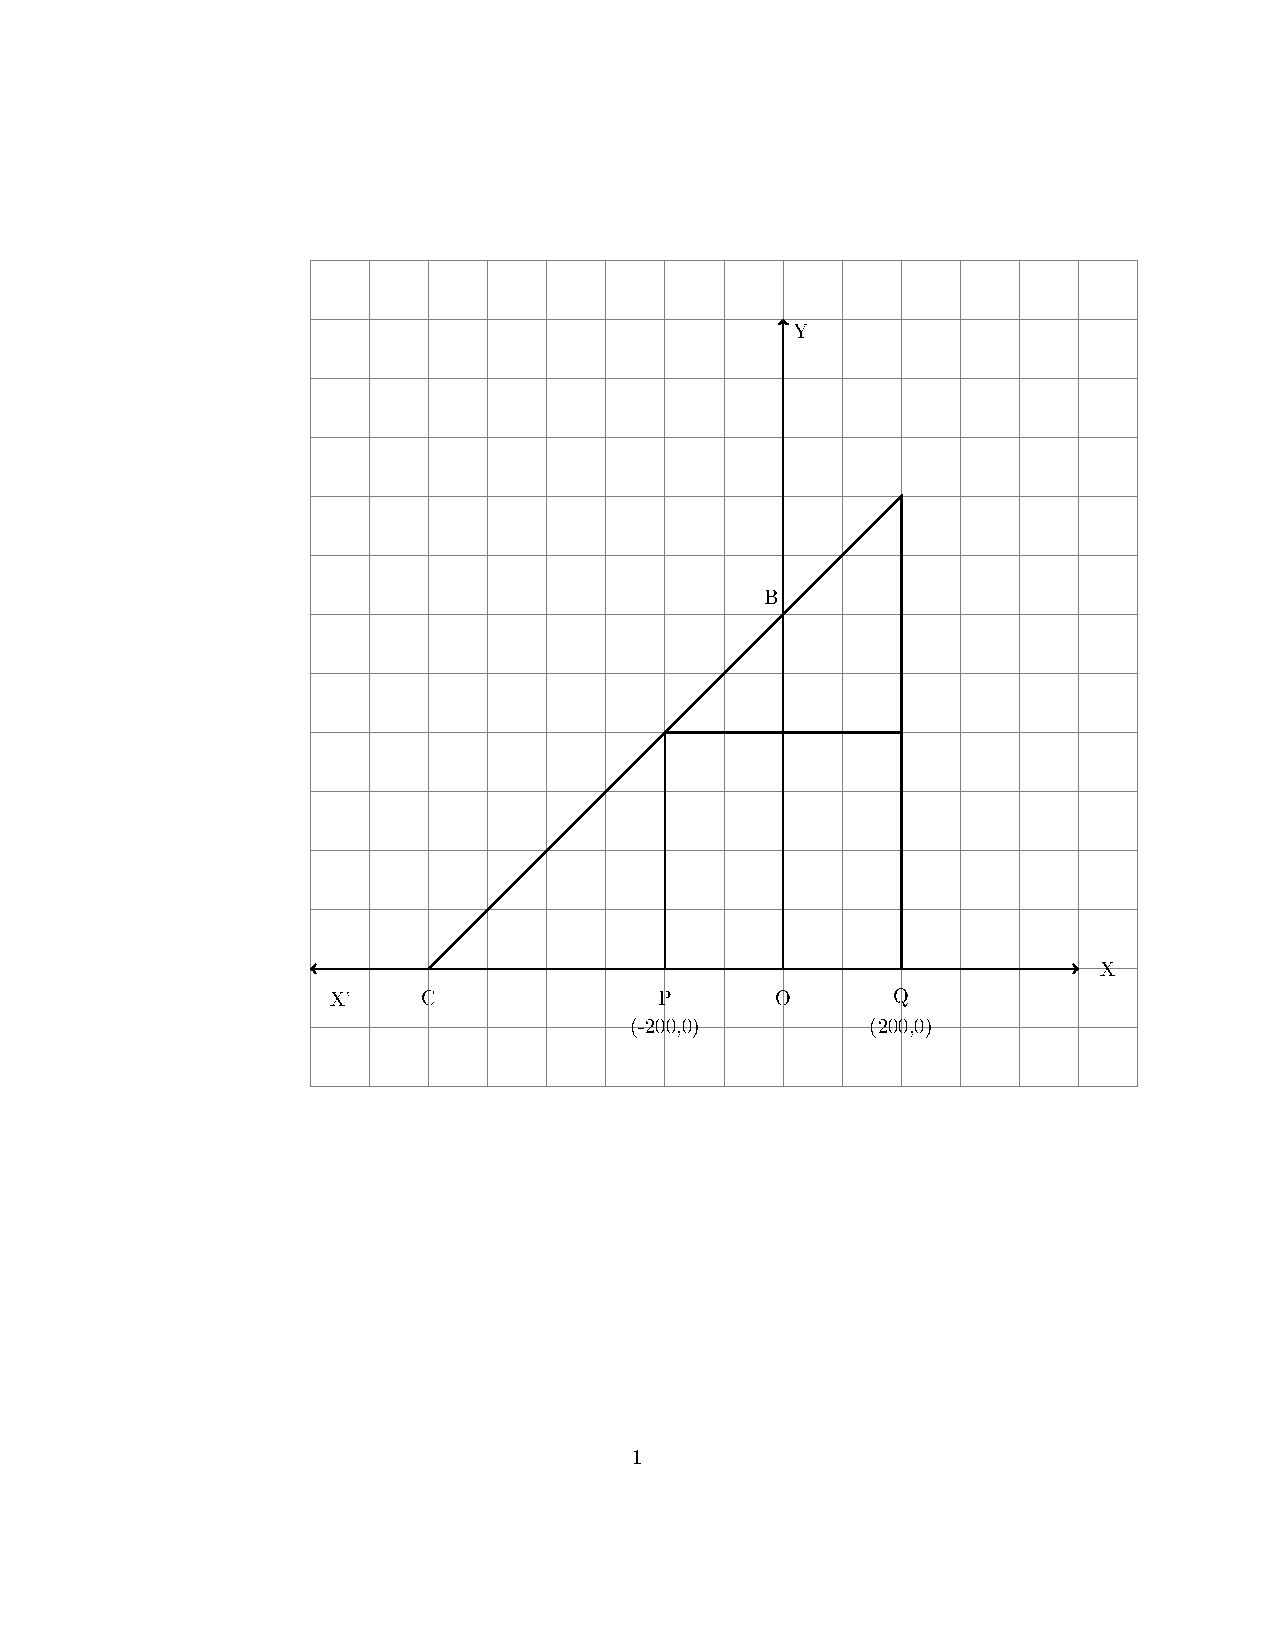
\includegraphics[width=\columnwidth]{figs/image}
 
  \caption{Image}
  \label{fig:1}
\end{figure}

Based on the above information,answer the following equations:
\begin{enumerate}
            \item Taking O as origin , coordinates of P are (-200,0) and of Q are (200,0). PQRS being a square, what are the coordinates of R and S?
            \item
            \begin{enumerate}
            \item What is the area of square PQRS?
            \item What is the length of diagonal PR in PQRS?
            \end{enumerate}
            \item If S divides CA in the ratio K:1,what is the value of K,where point A is (200,800)?
        \end{enumerate}
\end{enumerate}


\subsection{12}
\begin{enumerate}[label=\thesection.\arabic*.,ref=\thesection.\theenumi]
\numberwithin{equation}{enumi}
\numberwithin{figure}{enumi}
\numberwithin{table}{enumi}


\item Unit vector along $\vec{PQ}$, where coordinates of $\vec{P}$ and $\vec{Q}$ respectively are (2,1,-1)and(4,4,-7), is
\begin{enumerate}
\item $2\hat{i}+3\hat{j}-6\hat{k}$
\item $-2\hat{i}-3\hat{j}+6\hat{k}$
\item $-\frac{2\hat{i}}{7}-\frac{3\hat{j}}{7}+\frac{6\hat{k}}{7}$
\item $\frac{2\hat{i}}{7}+\frac{3\hat{j}}{7}-\frac{6\hat{k}}{7}$
\end{enumerate}

\item If in $\triangle$ABC, $\overrightarrow{BA}$=2$\overrightarrow{a}$ and $\overrightarrow{BC}$=3$\overrightarrow{b}$, then $\overrightarrow{AC}$ is
\begin{enumerate}
\item $2\overrightarrow{a}$ + 3$\overrightarrow{b}$
\item $2\overrightarrow{a}$ - 3$\overrightarrow{b}$
\item $3\overrightarrow{b}$ - 2$\overrightarrow{a}$
\item $-2\overrightarrow{a}$ -3$\overrightarrow{b}$
\end{enumerate}

\item Equation of line passing through origin and making 30\degree{}, 60\degree{} and 90\degree with x, y, z axes respectively is
\begin{enumerate}
\item $\frac{2x}{\sqrt{3}}$=$\frac{y}{2}$=$\frac{z}{0}$
\item $\frac{2x}{\sqrt{3}}$=$\frac{2y}{1}$=$\frac{z}{0}$
\item 2x=$\frac{2y}{\sqrt{3}}$=$\frac{z}{1}$
\item $\frac{2x}{\sqrt{3}}$=$\frac{2y}{1}$=$\frac{z}{1}$
\end{enumerate}

\item If $\overrightarrow{a}, \overrightarrow{b}, \overrightarrow{c}$ are three non-zero unequal vectors such that $\overrightarrow{a}.\overrightarrow{b}$ = $\overrightarrow{a}.\overrightarrow{c}$, then find the angle between $\overrightarrow{a}$ and $\overrightarrow{b}$ - $\overrightarrow{c}$.


\item If the equation of a line is
       \begin{align}
	x = ay + b, z = cy +d,
       \end{align}  then find the direction ratios of the line and a point on the line.

\item Using Integration, find the area of triangle whose vertices are (-1, 1), (0, 5) and (3, 2).


\end{enumerate}


\section{2022}
\subsection{10}
\begin{enumerate}[label=\thesection.\arabic*.,ref=\thesection.\theenumi]
\numberwithin{equation}{enumi}
\numberwithin{figure}{enumi}
\numberwithin{table}{enumi} 
\item The distance between the points $(0,0)$ and $(a-b, a+b)$ is 
\begin{enumerate}
\item $2{\sqrt{ab}}$
\item $\sqrt{2a^2 + ab}$
\item $ 2\sqrt{a^2 + b^2}$
\item $ \sqrt{2a^2 + 2b^2}$
\end{enumerate}
\item The value of m which makes the point $(0,0)$ , $(2m, -4)$ and $(3,6)$ collinear, is $\underline{\hspace{1cm}}$
\item A circle has its center at $(4,4)$. If one end of a diameter is $(4,0)$, then find the coordinates of other end.
\item  Find the area of the quadrilateral ABCD whose vertices are $A(-4, -3)$ , $B(3, -1)$, $C(0, 5)$ and $D(-4, 2)$
\item If the points $\vec{A}(2,0)$, $\vec{B}(6,1)$, and $\vec{C}(p ,q)$ form a triangle of area 12sq. units (positive only) and \begin{align}2p + q = 10\end{align}, then find the values of p and q.
\end{enumerate}


\subsection{12}
\begin{enumerate}[label=\thesection.\arabic*.,ref=\thesection.\theenumi]
\numberwithin{equation}{enumi}
\numberwithin{figure}{enumi}
\numberwithin{table}{enumi}
\item $\overrightarrow{a}$   and  $\overrightarrow{ b}$ are two unit vectors such that \begin{align} \abs { 2\overrightarrow{ a}+3\overrightarrow{ b}} = \abs{3\overrightarrow{ a} - 2\overrightarrow{ b}}. \end{align} Find the angle between $\overrightarrow{ a }$ and $\overrightarrow{ b }$.
\item If $\overrightarrow{ a}$  and $\overrightarrow{b}$ are two vectors such that  \begin{align}\overrightarrow{a} = \hat{i} - \hat{j} + \hat{k} \end{align}and  \begin{align}\overrightarrow{b} = 2\hat{i} - \hat{j} - 3\hat{k}\end{align} then find the vector $\overrightarrow{c}$, given that \begin{align}\overrightarrow{a} \times \overrightarrow{c} = \overrightarrow{b}\end{align}  and \begin{align}\overrightarrow{a}.\overrightarrow{c}= 4.\end{align}
\item \begin{align} If \abs{\overrightarrow{ a } \times \overrightarrow { b }}^2 + \abs { \overrightarrow{ a } . \overrightarrow{ b }}^2= 400 \end{align} and  \begin{align}\abs { \overrightarrow{ b}} = 5 \end{align} find the value of  $\abs{\overrightarrow{ a }}$. 
\item If \begin{align}\overrightarrow{a} = \hat{i} + \hat{ j} + \hat{ k} , \overrightarrow{a} . \overrightarrow{b} = 1\end{align}  and \begin{align}\overrightarrow{a} \times \overrightarrow{b} = \hat{j} - \hat{k}\end{align},  then find  $\abs{\overrightarrow{b}}$ 
\item If \begin{align}\abs{\overrightarrow{ a}}= 3, \abs{\overrightarrow{ b}} = 2\sqrt{ 3}\end{align}  and \begin{align}\overrightarrow{ a} . \overrightarrow{ b} = 6,\end{align}then find the value of $\abs{\overrightarrow{ a} \times \overrightarrow{ b}}$.
\item $\abs{\overrightarrow{a}} = 8, \abs{\overrightarrow{ b}} = 3$ and $\overrightarrow{a} . \overrightarrow{b} = 12\sqrt{3}$, then the value of  $\abs{\overrightarrow{a} \times \overrightarrow{b}}$ is
\begin{enumerate}                                      
\item  24                                              
\item  144                                             
\item  2                                              
\item  12                                             
\end{enumerate}
\item If$\space$ \begin{align}\overrightarrow{ a} = 2\hat{i} + \hat{j} + 3\hat{k}, \hat{b} = -\hat{i} + 2\hat{j} + \hat{k}\end{align} and \begin{align}\overrightarrow{c} = 3\hat{i} + \hat{j} + 2\hat{k}\end{align}, then find $\overrightarrow{a} . (\overrightarrow{ b} \times \overrightarrow{c})$. 
\item $\overrightarrow{a}, \overrightarrow{ b },\overrightarrow{ c }$  and  $\overrightarrow{ d }$ are four non-zeros vectors such that  $\overrightarrow{a}\times \overrightarrow{b}= \overrightarrow{c} \times \overrightarrow{d}$  and  \begin{align}\overrightarrow{a} \times \overrightarrow{c} = 4\overrightarrow{b} \times \overrightarrow{d}\end{align}, then show that  $(\overrightarrow{ a}-2\overrightarrow{d} \text{ is parallel to}(2\overrightarrow{b}-\overrightarrow{c})$ where \begin{align}\overrightarrow{a} \neq 2\overrightarrow{d}, \overrightarrow{c} \neq 2\overrightarrow{b}\end{align}
\item If \begin{align}\overrightarrow{a} = \hat{i} + \hat{ j} + \hat{ k} , \overrightarrow{a} . \overrightarrow{b} = 1\end{align}  and \begin{align}\overrightarrow{a} \times \overrightarrow{b} = \hat{j} - \hat{k},\end{align}  then find  $\abs{\overrightarrow{b}}$
\item  If $\overrightarrow{ a}$  and  $\overrightarrow{b}$  are two vectors such that \begin{align}\abs{\overrightarrow{a} + \overrightarrow{b}} = \abs{ \overrightarrow{b}},\end{align}then prove that $(\overrightarrow{a} + 2\overrightarrow{b})$  is perpendicular to $\overrightarrow{ a}$.
\item If $\overrightarrow{ a}$ and $\overrightarrow{ b}$ are unit vectors and $\theta$ is the angle between them , then prove that sin \begin{align}\dfrac{\theta}{ 2} = \dfrac{1}{2}\abs{\overrightarrow{ a} - \overrightarrow{ b}}\end{align}
\item If $\overrightarrow{a}$ and $\overrightarrow{b}$  are two unit vectors such that and $\theta$ is the ang le between them, then prove that                       \begin{align}sin \dfrac{ \theta}{2} = \dfrac{1}{2} \abs{\overrightarrow{a} - \overrightarrow{b}} \end{align} 
\item If \begin{align}\overrightarrow{a} = 2\hat{i} + y\hat{j} + \hat{ k}\end{align} and \begin{align}\overrightarrow{ b} = \hat{i} + 2\hat{j}+ 3\hat{k}\end{align} are two vectors for which the vector $(\overrightarrow{a}+\overrightarrow{b})$ is perpendicular to the vector  $(\overrightarrow{a}-\overrightarrow{b})$ then find all the possible values of y.
\item Write the projection of the vector $(\overrightarrow{b}+\overrightarrow{c})$  on the vector  $\overrightarrow{a}$ ,  where \begin{align}\overrightarrow{ a} = 2\hat{i}-2\hat{j}+\hat{k}, \overrightarrow{b} = \hat{i}+2\hat{j}-2\hat{k}\end{align} and \begin{align}\overrightarrow{c} = 2\hat{i}-\hat{j}+4\hat{k}.\end{align}
\item If \begin{align}\overrightarrow{ a } = 2\hat{i} - \hat{ j } +\hat{ k }, \overrightarrow{ b } = \hat{ i } + \hat{ j} - 2\hat{ k }\end{align} and  \begin{align}\overrightarrow{ c } = \hat{ i } +3\hat{j} - \hat{k}\end{align} and the projection of vector   $\overrightarrow{c} + \lambda \overrightarrow{b}$  on  vector  $\overrightarrow{a}$  is $2\sqrt{6}$, find the value of $\lambda$.
\item If$\space$ $\overrightarrow{ a} = 2\hat{i} + \hat {j} +3\hat{k}, \hat{b} = -\hat{i} + 2\hat{j} + \hat{k }$ and  \begin{align}\overrightarrow{c} = 3\hat{i} + \hat{j} + 2\hat{k}\end{align}, then find $\overrightarrow{a} . (\overrightarrow{ b} \times \overrightarrow{c})$.
\item If $\space$  \begin{align}\overrightarrow { a} = 2\hat{i} - \hat{j} + 2\hat{k}\end{align} and \begin{align}\overrightarrow{ b } = 5\hat{ i } -3\hat{j} -4\hat{k}\end{align}, then find the ratio $\dfrac{ projection  of vector\space \overrightarrow{ a }\space on vector \overrightarrow{ b }}{projection of vector \space \overrightarrow{ b }\space on  vector\space \overrightarrow{ a }}$	
\item Show that the three vectors $2\hat{ i} - \hat{j}  + \hat{k} , \hat{i} - 3\hat{j} - 5\hat{k}$ , and $3\hat{i} - 4\hat{j} - 4\hat{k}$ form the vertices of a right-angled triangle. If $\overrightarrow{ a} = 2\hat{i} + 2\hat{j} + 3\hat{k }, \overrightarrow{ b} = -\hat{i} + 2\hat{j} + \hat{ k }$  and  \begin{align}\overrightarrow{ c} = 3\hat{i} + \hat{ j}\end{align} are such that the vector  $(\overrightarrow{ a} + \lambda \overrightarrow{ b})$ is perpendicular to vector $\overrightarrow{ c}$, then find the value of $\lambda$.	
\item If $\overrightarrow{a} , \overrightarrow{b}$ and  $\overrightarrow{c}$ are the position vectors of the points $\vec{A}(2, 3, -4)$, $\vec{B}(3, -4, -5)$ and $\vec{C}(3, 2,-3)$ and respectively, then $\abs{\overrightarrow{a} + \overrightarrow{b} + \overrightarrow{c}}$ is equal to              
\begin{enumerate}                                     
\item $\sqrt{113}$                                     
\item $\sqrt{185}$                                     
\item $\sqrt{203}$                                     
\item $\sqrt{209}$                                    
\end{enumerate}
\item $\vec{A}$ circle has its center at $(4,4)$. If one end ofa diameter is $(4,0)$, then find the coordinates ofother end.
\item Find the values $\lambda$, for which the distance of point $( 2,1, \lambda)$ from plane \begin{align}3x+5y+4z=11\end{align} is $2\sqrt{2}$ units.                            
\item Find the coordinates of the point where the line through $(3,4,1)$ crosses the ZX-plane
\item Using vectors, find the area of the triangle withvertices $\vec{A}(-1, 0, -2)$, $\vec{B}(0, 2, 1)$ and $\vec{C}(-1, 4,1)$ 
\item Using integration, find the area of triangle region whose vertices are $(2,0)$ , $(4,5)$ and $(1,4)$.
\item The distance between the points $(0,0)$ and $(a-b, a+b)$ is                                             
\begin{enumerate}                                     
\item $2{\sqrt{ab}}$                                  
\item $\sqrt{2a^2 + ab}$                              
\item $ 2\sqrt{a^2 + b^2}$                            
\item $ \sqrt{2a^2 + 2b^2}$                           
\end{enumerate}                                       
\item The value of m which makes the point $(0,0)$ , $( 2m,-4)$and $(3,6)$ collinear, is $\underline{\hspace{1cm}}$
\item  If a line makes $60\degree$  and $45\degree$ angles with the positive directions of X-axis and z-axis respectively, then find the angle that it makes with the positive direction of y-axis. Hence, write the direct6on cosines of the line.
\item The Cartesian equation of a line $AB$ is :         \begin{align}\dfrac{2x-1}{12} = \dfrac{ y+2}{2} = \dfrac{z-3}{3}\end{align}.                        
\item Find the directions cosines of a line parallel to line $AB$.                                             
\item Find the direction cosines of a line whose cartesian equation is given as \begin{align}3x + 1 = 6y - 2 = 1 - z.\end{align}  
\item A vector of magnitude $9$ units in the direction of the vector $-2\hat{i} - \hat{j} + 2\hat{k}$ is \underline{\hspace{1cm}}
\item The two adajacent sides of a parallelogram are represented by $2\hat{i}-4\hat{j}-5\hat{k}$ and $\hat{ i}+2\hat{j}+3\hat{k}$. Find the unit vectors parallel to its diagonals. Using the diagonal vectors, find the area of the parallelogram also.                           
\item The two adjacent sides of a parallelogram are represented by vectors $2\hat{i} - 4\hat{j} + 5\hat{k}$  and  $\hat{ i} - 2\hat{j} - 3\hat{k}$. Find the unit vector parallel to one of its diagonals. Also,find the area of the parallelogram.                               
\item If $\space$ \begin{align}\overrightarrow{ a} = \overrightarrow{i} + 2\overrightarrow{j} + 3\overrightarrow{k}\end{align}   and \begin{align}\overrightarrow{ b} = 2\hat{i} + 4\hat{j} - 5\hat{k}\end{align} represent two adjacent sides of a parallelogram, then find the unit vector parallel to the diagonal of the parallelogram
\item  Find the area of the quadrilateral $ABCD$ whose vertices are $\vec{A}(-4, -3)$ , $\vec{B}(3, -1)$, $\vec{C}(0, 5)$ and $\vec{D}(-4, 2)$                                         
\item If the points $\vec{A}(2,0)$, $\vec{B}(6,1)$, and $\vec{C}(p ,q)$ form a triangle of area 12sq. units (positive only) and \begin{align}2p + q = 10,\end{align}then find the values of p and q.
\end{enumerate}



\section{2021}
\subsection{10}
\begin{enumerate}[label=\thesection.\arabic*.,ref=\thesection.\theenumi]		
\numberwithin{equation}{enumi}
\numberwithin{figure}{enumi}
\numberwithin{table}{enumi}
	\item Find the distance between the points $\vec{A}(-\frac{7}{3},5)$ and $\vec{B}(\frac{2}{3},5)$.                  	\item Check whether $13$cm, $12$cm, $5$cm can be the sides of a right triangle.
	\item \begin{enumerate}[label=(\alph*)]
			\item If $PL$ and $PM$ are two tangents to a circle with centre $\vec{O}$ from an external point $\vec{P}$ and $PL=4$ cm, find the length of $OP$, where radius of the circle is 3 cm.
		\item Find the distance between two parallel tangents of a cicle of radius $2.5$ cm.
             \end{enumerate}
     \item Find the coordinates of the points which divides the line segment joining the points $\vec{A}(7,-1)$ and $\vec{B}(-3,-4)$ in the ratio $2:3$.	
     \item To divide a line segment $QP$ internally in the ratio $2:3$, we draw a ray $QY$ such that $\angle$ PQY is acute. What will be  the minimum number of points to be located at equal distances on the ray $QY$ ?
     \item Answer any four of the following questions :
	     \begin{enumerate}[label=(\roman*)]
		     \item The point which divides the line segment joining the points $(7,-6)$ and $(3,4)$ in the ratio $1:2$ lies in
			     \begin{enumerate}[label=(\Alph*)]
                              \item \romanNumeral{1} quadrant
			      \item \romanNumeral{2} quadrant
			      \item \romanNumeral{3} quadrant
			      \item \romanNumeral{4} quadrant
			     \end{enumerate}
		     \item If the $\vec{A}(1, 2)$, $\vec{O}(0, 0)$ and $\vec{C}(a, 6)$ are collinear, then the value of a is
			     \begin{enumerate}[label=(\Alph*)]
				     \item $6$
				     \item $\frac{3}{2}$
				     \item $3$
				     \item $12$
			     \end{enumerate}
		    \item The distance between the points $\vec{A}(0, 6)$ and $\vec{B}(0, -2)$ is 
			    \begin{enumerate}[label=(\Alph*)]
				    \item $6$ units
				    \item $8$ units
				    \item $4$ units
				    \item $2$ units
				    \end{enumerate}
		    \item If $(\frac{a}{3},4)$ is the mid-point of the line segment joining the points $(-6, 5)$ and $(-2, 3)$, then the value of \lq a \rq{} is
		    \begin{enumerate}[label=(\Alph*)]
				    \item $-4$
				    \item $4$
				    \item $-12$
				    \item $12$
			    \end{enumerate}
		    \item What kind of triangle is formed with vertices $\vec{A}(0, 2)$, $\vec{B}(-3, 0)$ and $\vec{C}(3, 0)$ ?
			    \begin{enumerate}[label=(\Alph*)]
				    \item A right triangle
				    \item An equilateral triangle
				    \item An isosceles triangle
				    \item A scalene triangle
			    \end{enumerate}
	     \end{enumerate}
     \item \begin{enumerate}[label=(\alph*)]
		     \item If the distance between the points $(k, -2)$ and $(3, -6)$ is $10$ units, find the positive value of k.
		     \item Find the length of the segment joining $\vec{A}(-6, 7)$ and $\vec{B}(-1, -5)$.Also, find the mid-point of $AB$. 
     \end{enumerate}
     \item A man goes $5$ metres due to West and then $12$ metres due North. How far is he from the starting point ?
     \item Students of a school are standing in rows and columns in their school playground to celebrate their annual sports day. $\vec{A}$, $\vec{B}$, $\vec{C}$ and $\vec{D}$ are the positions of four students as shown in the figure. \\
	     	     \begin{figure}[ht]
		     \centering
		     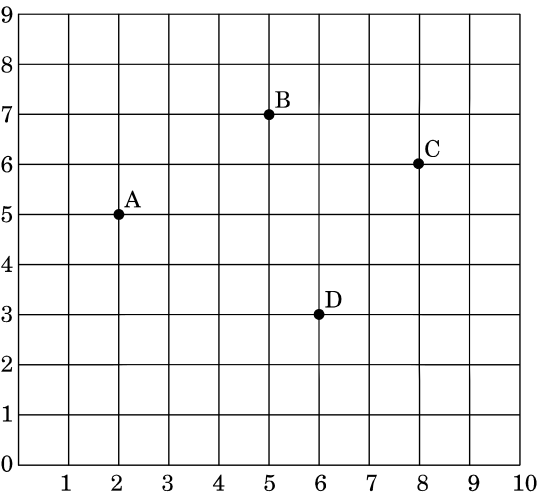
\includegraphics[width=0.45\columnwidth,height=0.45\columnwidth]{figs/fwc3.png}
		     \caption{Based on the above, answer the following question :}
		     \label{fig:my_label}
	     \end{figure}
\begin{enumerate}[label=(\roman*)]
	\item The figure formed by the points $\vec{A}$, $\vec{B}$, $\vec{C}$ and $\vec{D}$ is a
		\begin{enumerate}[label=(\Alph*)]
			\item sqaure
			\item parallelogram
			\item rhombus
			\item quadrilateral
		\end{enumerate}
	\item If the sports teacher is sitting at the origin, then which of the four students is closest to him ?
		\begin{enumerate}[label=(\Alph*)]
			\item $\vec{A}$
			\item $\vec{B}$
			\item $\vec{C}$
			\item $\vec{D}$
		\end{enumerate}
	\item The distance between $\vec{A}$ and $\vec{C}$ is 
		\begin{enumerate}[label=(\Alph*)]
			\item $\sqrt{37}$ units
			\item $\sqrt{35}$ units
			\item $6$ units
			\item $5$ units
		\end{enumerate}
	\item The coordinates of the mid-point of line segment $AC$ are
	\item If a point $\vec{P}$ divides the line segment $AD$ in the ratio $1:2$, then coordinates of $\vec{P}$ are
		\begin{enumerate}[label=(\Alph*)]
			\item $(\frac{8}{3},\frac{8}{3})$
			\item $(\frac{10}{3},\frac{13}{3})$
			\item $(\frac{13}{3},\frac{10}{3})$
			\item $(\frac{16}{3},\frac{11}{3})$
	\end{enumerate}
\end{enumerate}
\item \begin{enumerate}[label=(\alph*)]
		\item Check whether the points $\vec{P}(5, -2)$, $\vec{Q}(6, 4)$ and $\vec{R}(7, -2)$ are the vertices of an isosceles triangle PQR.
		\item Find the ratio in which $\vec{P}(4, 5)$ divides the join of $\vec{A}(2, 3)$ and $\vec{B}(7, 8)$.
\end{enumerate}
\item The coordinate of the three consecutive vertices of a parallelogram ABCD are $\vec{A}(1, 3)$, $\vec{B}(-1, 2)$, and $\vec{C}(2, 5)$. Find the cordinates of the fourth vertex $\vec{D}$.
\item \begin{enumerate}[label=(\alph*)]
		\item If $\vec{P}(2, 2)$, $\vec{Q}(-4, -4)$ and $\vec{R}(5, -8)$ are the vertices of a $\triangle$PQR, then find the length of the median through $\vec{R}$.
		\item Find the ratio in which y-axis divides the line segment joining the points $\vec{A}(5, -6)$ and $\vec{B}(-1, -4)$.Also, find the coordinates of the point of intersection.
\end{enumerate}
\item
	\begin{enumerate}[label=(\alph*)]
		\item Find the ratio in which the line segment joining the points $\vec{A}(1, -5)$ and $\vec{B}(-4, 5)$ is divided by the ax-axis. Also, find coordinates of the point of division.
		\item The points $\vec{A}(0, 3)$, $\vec{B}(-2, a)$ and $\vec{C}(-1, 4)$ are the vertices of a rigth triangle, right-angled at $\vec{A}$. Find the value of a. 
	\end{enumerate}
\end{enumerate}

\subsection{12}

\begin{enumerate}
	\item If $ \vec{a},\vec{b}, \vec{c} $ are position vectors of the points A(2,3,-4), B(3,-4,-5) and C(3,2,-3) respectively, then $ \abs{\vec{a}+\vec{b}+\vec{c}} $ is equal to
		\begin{enumerate}
			\item $\sqrt{113}$
			\item $\sqrt{185}$
			\item $\sqrt{203}$
			\item $\sqrt{209}$
		\end{enumerate}
\item Find the distance of the point (a,b,c) from the x-axis
\item If $ \vec{a}=2\hat{i}-\hat{j}+2\hat{k} $ and $ \vec{b}=5\hat{i}-3\hat{j}-4\hat{k} $, then find the ratio\text{$ \frac{\text{projection of vector  }\vec{a} \text{ on } \vec{b}}{\text{projection of vector } \vec{b} \text{ on vector } \vec{a}} $}
\item Let $\hat{a}$ and $\hat{b}$  be two unit vectors. If the vectors $\vec{c}=\hat{a}+2\hat{b}$ and $\vec{d}=5\hat{a}-4\hat{b}$ are perpendicular to each other, then find the angle between the vectors $\hat{a}$ and $\hat{b}$.
\item Show that $ \abs{\vec{a}} \vec{b}$ + $ \abs{\vec{b}} \vec{a}$ is perpendicular to $\abs{\vec{a} \vec{b}} $- $ \abs{\vec{b}} \vec{a} $, for any two non-zero vectors $\vec{a}$ and $\vec{b}$.
\item Prove that three points A,B and C with position vectors $\vec{a}, \vec{b}$ and $\vec{c}$ respectively are collinear if and only if $( \vec{b} \times \vec{c})+(\vec{c} \times \vec{a})+(\vec{a} \times \vec{b}) = \vec{0}$.
\end{enumerate}
\section{2019}
\subsection{12}
 \begin{enumerate}
 \item A line passes through the point with position vector $2\hat{i}-\hat{j}+4\hat{k}$ and is in the direction of the vector $\hat{i}+\hat{j}-2\hat{k}$. Find the equation of the line in cartesian form.
 
\item If ${\overrightarrow{\mydet{a}}}$ = $2, {\overrightarrow{\mydet{b}}}$ = $7$ and $\overrightarrow{a}\times\overrightarrow{b}$ = $3\hat{i}+2\hat{j}+6\hat{k}$, find the angle between $\overrightarrow{a}$ and $\overrightarrow{b}$.

\item Find the volume of a cuboid whose edges are given by $-3\hat{i}+7\hat{j}+5\hat{k}$,$-5\hat{i}+7\hat{j}-3\hat{k}$ and $7\hat{i}-5\hat{j}-3\hat{k}$.


\item The scalar product of the vector $\overrightarrow{a} = \hat{i}+\hat{j}+\hat{k}$ with a unit vector along the sum of the vectors $\overrightarrow{b} = 2\hat{i}+4\hat{j}-5\hat{k}$ and $\overrightarrow{c} = \hat{\lambda}+2\hat{j}+3\hat{k}$ is equal to $1$. Find the value of $\lambda$ and hence find the unit vector along $\overrightarrow{b}+\overrightarrow{c}$.

\item Find the vector and cartesian equations of the plane passing through the points having position vectors $\hat{i}+\hat{j}-2\hat{k}$, $2\hat{i}-\hat{j}+\hat{k}$ and $\hat{i}+2\hat{j}+\hat{k}$. Write the equation of a plane passing through a point \myvec{2, 3, 7} and parallel to the plane obtained above. Hence, find the distance between the two parallel planes.

\item Find the cartesian and vector equations of the plane passing through the points $A$\brak{2,5,-3}, $B$\brak{-2,-3,5} and $C$\brak{5,3,-3}.

 \item Show that the points $A\brak{-2\hat{i}+3\hat{j}+5\hat{k}}$, $B\brak{\hat{i}+2\hat{j}+3\hat{k}}$ and $C\brak{7\hat{i}-\hat{k}}$ are collinear.
 
 \item Find $\mydet{\overrightarrow{a}\times\overrightarrow{b}}$, if $\overrightarrow{a}=2\hat{i}+\hat{j}+3\hat{k}$ and $\overrightarrow{b}=3\hat{i}+5\hat{j}-2\hat{k}$.
 
 \item Using integration, find the area of the triangular region whose sides have the equations ${y}={2x}+1$, ${y}={3x}+1$ and ${x}=4$.

 \item Using method of integration, find the area of the triangle whose vertices are $\myvec{1,0}$,$\myvec{2,2}$ and $\myvec{3,1}$.
 
 \item Find the direction cosines of a line which makes equal angles with the coordinate axes.
         
 \item If the lines $\frac{x-1}{-3}=\frac{y-2}{2\lambda}=\frac{z-3}{2}$ and $\frac{x-1}{3\lambda}=\frac{y-1}{2}=\frac{z-6}{-5}$ are perpendicular, find the value of $\lambda$. Hence find weather the lines are intersecting or not.
           
\item Find the equation of the line passing through \brak{2, – 1, 2} and \brak{5, 3, 4} and of the plane passing through \brak{2, 0, 3}, \brak{1, 1, 5} and \brak{3, 2, 4}. Also, find their point of intersection.
\end{enumerate}


\item Find the value of $\lambda$ for which the following lines are perpendicular to each other :
\begin{align*}
    \dfrac{x-5}{5{\lambda+2}}=\dfrac{2-y}{5}=\dfrac{1-z}{-1};\dfrac{x}{1}=\dfrac{y+\dfrac{1}{2}}{2{\lambda}}=\dfrac{z-1}{3}.
\end{align*}
Hence, find whether the lines intersect or not.

\item Find the value of $p$ for which the following lines are perpendicular :
\begin{align*}
\dfrac{1-x}{3}= \dfrac{2y-14}{2p} = \dfrac{z-3}{2}; \dfrac{1-x}{3p} = \dfrac{y-5}{1} = \dfrac{6-z}{5}.
\end{align*}

\item Find the vector and Cartesian equations of the plane passing through the points $\brak{2,5,-3},\brak{-2,-3,5},$ and $\brak{5,3,-3}$.Also, find the point of intersection of this plane with the line passing through points $\brak{3,1,5} $ and $\brak{-1,-3,-1}.$

\item If a line has the direction ratios $-18, 12, -4,$ then what are its direction cosines ? 

\item Find the equation of the plane passing through the intersection of the planes $\overrightarrow r.\brak{\hat{i}+\hat{j}+\hat{k}}=1 $ and$\overrightarrow  r .2\hat{i}+3\hat{j}-\hat{k}+4=0 $ and parallel to $x-axis$. Hence, find the distance of the plane from $x-axis$.

\item Find the Cartesian equation of the line which passes through the point $\brak{- 2, 4,-5}$ and is parallel to the line 
\begin{align*}
\dfrac{x+3}{3}=\dfrac{4-y}{5}=\dfrac{z+8}{6}.
\end{align*}

\item Find a unit vector perpendicular to both the vectors 
$ \overrightarrow a $ and $ \overrightarrow b $ , where $ \overrightarrow a $ = $\hat{i} -7\hat{j} +7\hat{k}$ and $ \overrightarrow b = 3 \hat{i} -2 \hat{j}+ 2 \hat{k}$.

\item Show that the vectors $\hat{i} -2 \hat{j}+ 3 \hat{k},-2 \hat{i}+ 3  \hat{j} -4 \hat{k}$ and $\hat{i} -3 \hat{j}+ 5 \hat{k}$ are coplanar.

\item Let  $ \overrightarrow a ,\overrightarrow b$ and $\overrightarrow c $ be three vectors such that $\mydet{\overrightarrow{a}}  = 1 ,\mydet{\overrightarrow{b}}= 2$ and $\overrightarrow{|c|} =3$ .If the projection of $\overrightarrow b $ along $\overrightarrow a $ is equal to the projection of $\overrightarrow c $ along $ \overrightarrow a $; and $\overrightarrow b,\overrightarrow c $ are perpendicular to each other, then find $\abs{3\overrightarrow a-2\overrightarrow b +2\overrightarrow c}$.

\item Find the direction cosines of the line joining the points $P \brak{4, 3, -5}$ and $Q  \brak{-2, 1, -8}$.

\item Find the area of the triangle whose vertices are $\brak{-1, 1},\brak {0, 5}$ and $\brak {3, 2}$,using integration.

\item Find the equation of planes passing through the intersection of planes$ \overrightarrow r.\brak{3\hat{i}+6\hat{j}}+12=0$ and $ \overrightarrow {r}.\brak{3\hat{i}-\hat{j}+4\hat{k}}=0$ and are at a unit distance from origin.                         
\item  Find the angle between the line $\overrightarrow{r}$ = $\brak{2\hat{i}-\hat{j}+\hat{k}}$+ $\lambda\brak{3\hat{i}-\hat{j}+2\hat{k}}$ and the plane $\overrightarrow{r}\cdot\brak{\hat{i} +\hat{j}+\hat{k}}=3$.
\item Find the co-ordinates of the point where the line $\dfrac{x+2}{1}=\dfrac{y-5}{3}=\dfrac{z+1}{5}$ cuts the $yz$-plane.
\item Using vectors, prove that the points $\brak{2,-1,3}$, $\brak{3,-5,1}$ and $\brak{-1,11,9}$ are co-linear.
\item For any two vectors $\overrightarrow{\vec{a}}$ and $\overrightarrow{\vec{b}}$ prove that 
	\begin{align*}	\brak{\overrightarrow{\vec{a}}\times\overrightarrow{\vec{b}}}^{2}=\overrightarrow{\vec{a}}^{2}\overrightarrow{\vec{b}}^{2}-\brak{\overrightarrow{\vec{a}}.\overrightarrow{\vec{b}}}^{2}
	\end{align*}                 
 \item Using integration, find the area of $\triangle$ $ABC$ bounded by the lines
\begin{align*}
4x-y+5&=0,\\x+y-5&=0,\\x-4y+5&=0.
\end{align*} 


 \item Let $\overrightarrow{a}=\hat{i}+2\hat{j}-3\hat{k}$ and $\overrightarrow{b}=3\hat{i}-\hat{j}+2\hat{k}$ be two vector. Show that vector $\brak{\overrightarrow{a}+\overrightarrow{b}}$ and $\brak{\overrightarrow{a}-\overrightarrow{b}}$ are perpendicular to each other. 

      \item $X$ and $Y$ are two points with position vectors $3\overrightarrow{a}+\overrightarrow{b}$ and $\overrightarrow{a}-3\overrightarrow{b}$ respectively. Write the position vector of a point $Z$ which divides the line segment $XY$ in the ratio $2:1$ externally.



 
\item Find the equation of the plane passing through the point $\brak{-1,3,2}$ and perpendicular to the planes $x+2y+3z=5$ and $3x+3y+z=0$.

\item Find the vector equation of the line passing through $\brak{2,1,-1}$ and parallel to the line $\overrightarrow{r}$=$\brak{\hat{i}+\hat{j}}+\lambda\brak{2\hat{i}-\hat{j}+\hat{k}}$. Also find the distance between these two lines.

 \item Find the equation of the plane passing through the point $(-1,3,2)$ and perpendicular to the planes $x+2y+3z=5$ and $3x+3y+z=0$.
 
\item Find the coordinates of the foot $Q$ of the perpendicular drawn from the point $P\brak{1,3,4}$ to the plane $2x-y+z+3=0$. Find the distance $PQ$ and the image of $P$ treating the plane as a mirror. 

\item Using vectors find the value of $\vec{x}$ such that the four points $A\brak{x,5,-1}$, $B\brak{3,2,1}$ ,$C\brak{4,5,5}$ and $D\brak{4,2,-2}$ are co-planar.

\end{enumerate}

\section{2019}
\subsection{10}
\begin{enumerate}
\item The point $R$ divides the line segment $AB$, where $A\brak{- 4, 0}$ and $B\brak{0, 6}$ such that $AR=\frac{3}{4} AB$. Find the coordinates of $R$.

\item In what ratio does the point $P\brak{- 4, y}$ divide the line segment joining the points $A\brak{- 6, 10}$ and $B\brak{3, - 8}$ ? Hence find the value of $y$.

\item Find the distance between the points $\brak{a, b}$ and $\brak{-a, -b}$.

\item Find the value of $p$ for which the points $\brak{-5, 1}$, $\brak{1, p}$ and $\brak{4, -2}$ are collinear.

\item Find the area of a triangle whose vertices are given as $\brak{1, - 1}, \brak{- 4, 6}$ and $\brak{ -3, - 5}$.

\item Write the coordinates of a point $P$ on x-axis which is equidistant from the points $A\brak{- 2, 0}$ and $B\brak{6, 0}$.

\item Find a relation between $x$ and $y$ if the points $A\brak{x, y}$,  $B\brak{-4, 6} $ and $C\brak{-2, 3}$ are collinear.

\item Point $\Vec{A}$ lies on the line segment $\Vec{XY}$ joining $X\brak{6, - 6}$ and $Y\brak{-4,-1}$ in such a way that $\frac{XA}{XY}=\frac{2}{5}$. If point $A$ also lies on the line $3x + k \brak{y + 1}= 0$, find the value of $k$.

\item Find the ratio in which the y-axis divides the line segment joining the points $\brak{-1, -4}$ and $\brak{5, -6}$. Also find the coordinates of the point of intersection.

\item Find the ratio in which the line $x-3y = 0$ divides the line segment joining the points $\brak{ -2, -5}$ and $\brak{6, 3}$. Find the coordinates of the point of intersection.

\item Find the value $\brak{s}$ of $x$, if the distance between the points $A\brak{0, 0}$ and $B \brak{x,-4}$  is $5$ units.

\item Points $A\brak{3, 1}, B\brak{5, 1},C\brak{a, b}$ and $D\brak{4, 3}$ are vertices of a parallelogram $ABCD$. Find the values of $a$ and $b$.

\item Points $P$ and $Q$ trisect the line segment joining the points $A\brak{-2, 0}$ and $B\brak{0, 8}$ such that $P$ is near to $A$. Find the coordinates of points $P$ and $Q$.

\item Find the area of the triangle formed by joining the mid-points of the sides of the triangle ABC, whose vertices are $A\brak{0, - 1}$, $B\brak{2, 1}$ and $C\brak{0, 3}$.

\end{enumerate}

\section{2018}
\subsection{10}
\begin{enumerate}
	\item $\vec{A}(-2,1), \vec{B}(a,0), \vec{C}(4,b)$ and  $\vec{D}(1,2)$ are the vertices of a parallelogram {ABCD}, find the values of $a$ and $b$. Hence find the lengths if its sides.
	\item $\vec{A}(-5,7), \vec{B}(-4,-5), \vec{C}(-1,-6)$ and $\vec{D}(4,5)$ are the vertices of a quadrilateral, find the area of the quadrilateral ABCD.

			\item Find the distance of a point $\vec{P}(x,y)$ from the origin.
			\item Find the ratio in which $\vec{P}(4,m)$ divides the line segment joining the points $\vec{A}(2,3)$ and $\vec{B}(6,-3)$. Hence find m.

		\section{Construction}
	\item In an equilateral $\triangle$ ABC, D is a point on side BC such that $ BD =\frac{1}{3}BC$. Prove that $9(AD)^2 = 7(AB)^2$.
	\item Prove that, in a right triangle, the  square on the hypotenuse is equal to sum of the squares on the other two sides.
	\item Prove that the area of an equilateral triangle described on one side of the square is equal to half of the area of the equilateral triangle described on one of its diagonal.
	\item If the area of two similar triangles are equal, prove that they are congruent.
	\item Draw a triangle ABC with $BC=6 cm, AB=5 cm$ and $\angle{ABC}=60\degree$. Then construct a triangle whose sides are $\frac{3}{4}$ of the corresponding sides of the $\triangle ABC$.

	\item Given $\triangle ABC \sim  \triangle PQR$, if $\frac{AB}{PQ} = \frac{1}{3}$, then find $\frac{ar \triangle ABC}{ar \triangle PQR}$.


\section{2018}
\begin{enumerate}
\section*{Vectors}

\item A line passes through the point with position vector 
$2\hat{i} - \hat{j} + 4\hat{k} $ and is the direction of the vector 
$\hat{i} + \hat{j} - 2\hat{k} $. 
Find the equation of the line in cartesian form.

\item Show that the points 
A\brak{-2\hat{i} + 3\hat{j} + 5\hat{k}},B\brak{\hat{i} + 2\hat{j} + 3\hat{k}}
and C\brak{7\hat{i} -\hat{k} } are collinear.

\item Find
$|\overrightarrow{a} \times \overrightarrow{b}|$,
if $\overrightarrow{a}=2\hat{i}+\hat{j}+3\hat{k}$ and
$\overrightarrow{b}=3\hat{i}+5\hat{j}-2\hat{k}$.   

\item The scalar product of the vector 
$\overrightarrow{a} = \hat{i} + \hat{j} + \hat{k}$
with a unit vector along the sum of the vector 
$\overrightarrow{b} = 2\hat{i} + 4\hat{j} - 5\hat{k}$ and
$\overrightarrow{c} = \lambda \hat{i} + 2\hat{j} + 3\hat{k}$ 
is equal to $1$. Find the value of $\lambda$ and hence find 
the unit vector along 
$\overrightarrow{b} + \overrightarrow{c}$.

\item Find the vector and cartesian equations of the plane
passing through the points having position vectors 
$\hat{i} + \hat{ j} - 2\hat{k}$, $2\hat{i}-\hat{j} + \hat{k}$ 
and $\hat{i} + 2\hat{j} + \hat{k}$. Write the equation of the 
plane passing through a point \brak{2,3,7} and parllel to 
the plane obtained above. Hence, find the distance between the 
two parallel planes.

\item Find the direction cosine of the line which makes 
equal angles with the coordinate axes. 

\item If the line 
$\dfrac{x-1}{-3} = \dfrac{y-2}{2\lambda} = \dfrac{z-3}{2} $ and 
$\dfrac{x-1}{3\lambda} = \dfrac{y-1}{2}  = \dfrac{z-6}{-5}$ 
are perpendicular, find the value of $\lambda$. 
Hence find whether the lines are intersecting or not.
\end{enumerate}





\chapter{Linear Forms}
\section{2023}
\subsection{10}

\begin{enumerate}



  \item \textbf{Assertion (A):} Point $\vec{P}$(0,2) is the point of intersection of $y-axis$ with  the line $3x+2y=4$.\\
    \textbf{Reason (R):} The distance of point $\vec{P}$(0,2) from $x-axis$ is 2 units.


  \item If the pair of equations $3x-y+8=0$ and $6x-ry+16=0$ represent coincident lines, then the value of \text{'$r$'} is:

    \begin{enumerate}
      \item $-\frac{1}{2}$
      \item $\frac{1}{2}$
      \item -2
      \item 2
    \end{enumerate}

  \item The of linear equations $2x=5y+6$ and $15y=6x-18$ represents two lines which are:

      \begin{enumerate}
        \item intersecting
        \item parallel
        \item coincident
        \item either intersecting or parallel
      \end{enumerate}

    \item Find the equations of the diagonals of the parallelogram $\vec{PQRS}$ whose vertices are $\vec{P}$(4,2,-6), $\vec{Q}$(5,-3,1), $\vec{R}$(12,4,5) and $\vec{S}$(11,9,-2). Use these equations to find the point of intersection of diagonals.

  \item A line $l$ passes through point (-1,3,-2) and is perpendicular to both the lines $\frac {x}{1}=\frac{y}{2}=\frac{z}{3}$ and $\frac {x+2}{-3}=\frac{y-1}{2}=\frac{z+1}{5}$. Find the ctor equation of the line $l$. Hence, obtain its distance from origin.

\end{enumerate}

\subsection{12}                                                                                                  
\documentclass[12pt,A4 paper]{article}
\usepackage{mathtools}
\usepackage{graphicx}
\usepackage{gensymb}
\begin{document}
\title{\textbf{LINEAR}}
\date{}
\maketitle
\begin{enumerate}
    \item Equation of line passing through origin and making $30\degree,60\degree$ and $90\degree$ with $x,y,z$ axes respectively is
    \begin{enumerate}
        \item $\frac{2x}{\sqrt3}=\frac{y}{2}=\frac{z}{0}$
        \item $\frac{2x}{\sqrt3}=\frac{2y}{1}=\frac{z}{0}$
        \item $2x=\frac{2y}{\sqrt3}=\frac{z}{1}$
        \item $\frac{2x}{\sqrt3}=\frac{2y}{1}=\frac{z}{1}$
    \end{enumerate}
    \item If the equation of a line is $x=ay+b,z=cy+d$,then find the direction ratios of the line and a point on the line.
    \item
    \begin{enumerate}
        \item Find the equations of the diagonals of the parallelogram $PQRS$ whose vertices are$P(4,2,-6),Q(5,-3,1),R(12,4,5),S(11,9,-2)$.Use these equations to find the point of intersection of diagonals.  
        \item A line $l$ passes through point$(-1,3,-2)$ and is perpendicular to both the lines $\frac{x}{1}=\frac{y}{2}=\frac{z}{3}$ and $\frac{x+2}{-3}=\frac{y-1}{2}=\frac{z+1}{5}$.Find the vector equation of the line $l$.Hence,obtain its distance from origin.
    \end{enumerate}
   
   
   
\end{enumerate}
\end{document}


\section{2022}
\begin{enumerate}[label=\thesection.\arabic*.,ref=\thesection.\theenumi]
\numberwithin{equation}{enumi}
\numberwithin{figure}{enumi}
\numberwithin{table}{enumi}

\item Solve the equations $x+2y=6$ and $2x-5y=12$ graphically.	

	\item Solve the following equations for $x$ and $y$ using cross-multiplication method:
		\begin{align}
			(ax-by)+(a+4b)=0\\(bx+ay)+(b-4a)=0
		\end{align}

	\item Find the co-ordinates of the point where the line $\dfrac{x-3}{-1}=\dfrac{y+4}{1}=\dfrac{z+5}{6}$ crosses the plane passing through the points $\left(\dfrac{7}{2},0,0\right),(0,7,0),(0,0,7)$.

	\item Electrical transmission wires which are laid down in winters are stretched tightly to accommodate expansion in summers.
		\begin{figure}[H]
			\centering
			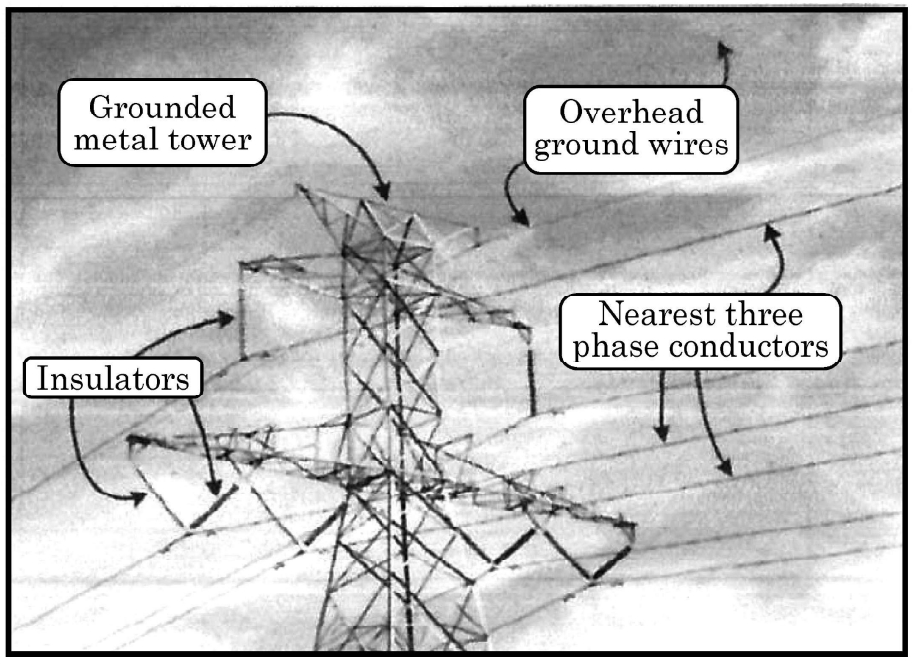
\includegraphics[width=\columnwidth]{figs/txn}
			\caption{Electrical transmission wires connected to a transmission tower.}
			\label{fig:txn1}
		\end{figure}
		Two such wires in the figure \ref{fig:txn1} lie along the following lines:
		\begin{align}
			l_1 &: \dfrac{x+1}{3}=\dfrac{y-3}{-2}=\dfrac{z+2}{-1}\\
			l_2 &: \dfrac{x}{-1}=\dfrac{y-7}{3}=\dfrac{z+7}{-2}
		\end{align}
		Based on the given information, answer the following questions:
		\begin{enumerate}
			\item	Are the $l_1$ and $l_2$ coplanar? Justify your answer.
			\item    Find the point of intersection of lines $l_1$ and $l_2$.
		\end{enumerate}

	\item Write the cartesian equation of the line PQ passing through points P$(2,2,1)$ and Q$(5,1,-2)$. Hence, find the y-coordinate of the point on the line PQ whose z-coordinate is -2.

	\item Find the distance between the lines $x=\dfrac{y-1}{2}=\dfrac{z-2}{3}$ and $x+1=\dfrac{y+2}{2}=\dfrac{z-1}{3}$.
	
	\item Find the shortest distance between the following lines:
		\begin{align}
			\vec{r}&=3\hat{i}+5\hat{j}+7\hat{k}+\lambda(\hat{i}-2\hat{j}+\hat{k})\\\vec{r}&=(-\hat{i}-\hat{j}-\hat{k})+\mu(7\hat{i}-6\hat{j}+\hat{k})
		\end{align}

	\item Two motorcycles A and B are running at a speed more than the allowed speed on the road (as shown in figure \ref{fig:bike1}) represented by the following lines 
		\begin{align}
			\vec{r}&=\lambda(\hat{i}+2\hat{j}-\hat{k})\\\vec{r}&=(3\hat{i}+3\hat{j})+\mu(2\hat{i}+\hat{j}+\hat{k})
		\end{align}
		\begin{figure}[H]
			\centering
			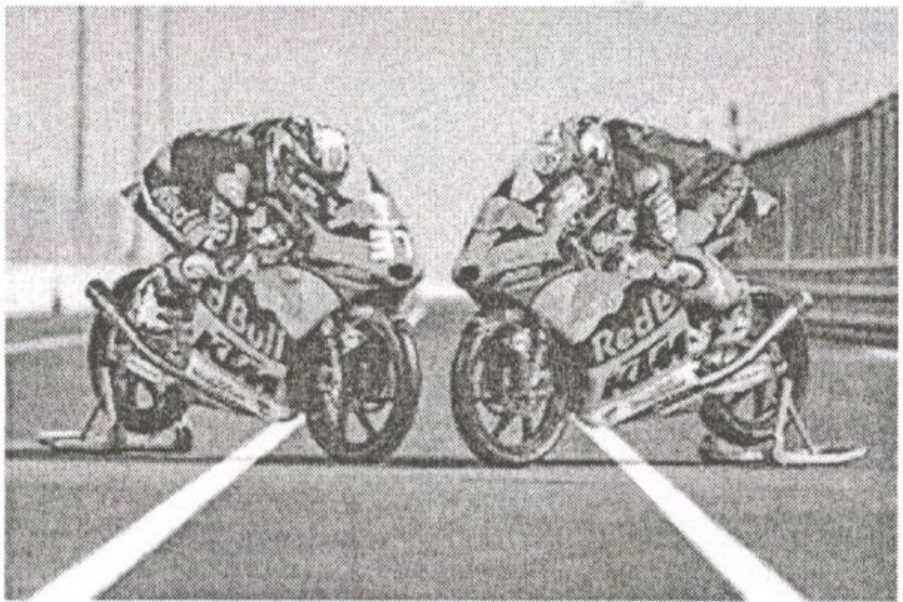
\includegraphics[width=\columnwidth]{figs/bike}
			\caption{Two motorcycles moving along the road in a straight line.}
			\label{fig:bike1}
		\end{figure}
		Based on the following information, answer the following questions:
		\begin{enumerate}
			\item Find the shortest distance between the given lines.
			\item Find a point at which the motorcycles may collide.
		\end{enumerate}
	
	\item Find the shortest distance between the following lines
		\begin{align}
			\vec{r}&=(\lambda+1)\hat{i}+(\lambda+4)\hat{j}-(\lambda-3)\hat{k}\\\vec{r}&=(3-\mu)\hat{i}+(2\mu+2)\hat{j}+(\mu+6)\hat{k}
		\end{align}
	
	\item Find the shortest distance between the following lines and hence write whether the lines are intersecting or not.
		\begin{align}
			\dfrac{x-1}{2}=\dfrac{y+1}{3}=z, \dfrac{x+1}{5}=\dfrac{y-2}{1}, z=2
		\end{align}

		\item Find the equation of the plane passing through the points $(2,1,0),(3,-2,-2)$ and $(1,1,7)$. Also, obtain its distance from the origin.

	\item The foot of a perpendicular drawn from the point $(-2,-1,-3)$ on a plane is $(1,-3,3)$. Find the equation of the plane.

	\item Find the cartesian and the vector equation of a plane which passes through the point $(3,2,0)$ and contains the line $\dfrac{x-3}{1}=\dfrac{y-6}{5}=\dfrac{z-4}{4}$.

	\item The distance between the planes $4x-4y+2z+5=0$ and $2x-2y+z+6=0$ is

		\begin{enumerate}

			\item $\dfrac{1}{6}$
			\item $\dfrac{7}{6}$
			\item $\dfrac{11}{6}$
			\item $\dfrac{16}{6}$
		\end{enumerate}

	\item Find the equation of the plane through the line of intersection of the planes
		\begin{align}
			\vec{r}\cdot(\hat{i}+3\hat{j})+6&=0\\\vec{r}\cdot(3\hat{i}-\hat{j}-4\hat{k})&=0
		\end{align}which is at a  unit distance from the origin.

		\item If the distance of the point $(1,1,1)$ from the plane $x-y+z+\lambda=0$ is $\dfrac{5}{\sqrt{3}}$, find the value(s) of $\lambda$.

	\item Find the distance of the point $(2,3,4)$ measured along the line $\dfrac{x-4}{3}=\dfrac{y+5}{6}=\dfrac{z+1}{2}$ from the plane $3x+2y+2z+5=0$.

	\item Find the distance of the point $P(4,3,2)$ from the plane determined by the points $A(-1,6,-5),B(-5,-2,3)$ and $C(2,4,-5)$.

	\item The distance of the line
		\begin{align}
		\vec{r}=(\hat{i}-\hat{j})+\lambda(\hat{i}+5\hat{j}+\hat{k})\end{align}
		from the plane
		\begin{align}
		\vec{r}\cdot(\hat{i}-\hat{j}+4\hat{k})=5\end{align}
		is
		\begin{enumerate}
			\item $\sqrt{2}$
			\item $\dfrac{1}{\sqrt{2}}$
			\item $\dfrac{1}{3\sqrt{2}}$
			\item $\dfrac{-2}{3\sqrt{2}}$
		\end{enumerate}

	\item Find a unit vector perpendicular to each of the vectors $(\vec{a}+\vec{b})$ and $(\vec{a}-\vec{b})$ where 
	\begin{align}
		\vec{a}&=\hat{i}+\hat{j}+\hat{k}\\\vec{b}&=\hat{i}+2\hat{j}+3\hat{k}
	\end{align}

	\item Find the distance of the point $(1,-2,9)$ from the point of intersection of the line
		\begin{align}
			\vec{r}=4\hat{i}+2\hat{j}+7\hat{k}+\lambda(3\hat{i}+4\hat{j}+2\hat{k})
		\end{align}and the plane
		\begin{align}
			\vec{r}\cdot(\hat{i}-\hat{j}+\hat{k})=10.
		\end{align}

	\item Find the area bounded by the curves $y=\abs{x-1}$ and $y=1$, using integration.

	\item Find the coordinates of the point where the line through $(4,-3,-4)$ and $(3,-2,2)$ crosses the plane $2x+y+z=6$.

	\item Fit a straight line trend by the method of least squares and find the trend value for the year 2008 using the data from Table \ref{tab:LC}:
		\begin{table}[H]
			\caption{Table showing yearly trend of production of goods in lakh tonnes \label{tab:LC}}
			%%%%%%%%%%%%%%%%%%%%%%%%%%%%%%%%%%%%%%%%%%%%%%%%%%%%%%%%%%%%%%%%%%%%%%
%%                                                                  %%
%%  This is the header of a LaTeX2e file exported from Gnumeric.    %%
%%                                                                  %%
%%  This file can be compiled as it stands or included in another   %%
%%  LaTeX document. The table is based on the longtable package so  %%
%%  the longtable options (headers, footers...) can be set in the   %%
%%  preamble section below (see PRAMBLE).                           %%
%%                                                                  %%
%%  To include the file in another, the following two lines must be %%
%%  in the including file:                                          %%
%%        \def\inputGnumericTable{}                                 %%
%%  at the beginning of the file and:                               %%
%%        \input{name-of-this-file.tex}                             %%
%%  where the table is to be placed. Note also that the including   %%
%%  file must use the following packages for the table to be        %%
%%  rendered correctly:                                             %%
%%    \usepackage[latin1]{inputenc}                                 %%
%%    \usepackage{color}                                            %%
%%    \usepackage{array}                                            %%
%%    \usepackage{longtable}                                        %%
%%    \usepackage{calc}                                             %%
%%    \usepackage{multirow}                                         %%
%%    \usepackage{hhline}                                           %%
%%    \usepackage{ifthen}                                           %%
%%  optionally (for landscape tables embedded in another document): %%
%%    \usepackage{lscape}                                           %%
%%                                                                  %%
%%%%%%%%%%%%%%%%%%%%%%%%%%%%%%%%%%%%%%%%%%%%%%%%%%%%%%%%%%%%%%%%%%%%%%



%%  This section checks if we are begin input into another file or  %%
%%  the file will be compiled alone. First use a macro taken from   %%
%%  the TeXbook ex 7.7 (suggestion of Han-Wen Nienhuys).            %%
\def\ifundefined#1{\expandafter\ifx\csname#1\endcsname\relax}


%%  Check for the \def token for inputed files. If it is not        %%
%%  defined, the file will be processed as a standalone and the     %%
%%  preamble will be used.                                          %%
\ifundefined{inputGnumericTable}

%%  We must be able to close or not the document at the end.        %%
 \def\gnumericTableEnd{\end{document}}


%%%%%%%%%%%%%%%%%%%%%%%%%%%%%%%%%%%%%%%%%%%%%%%%%%%%%%%%%%%%%%%%%%%%%%
%%                                                                  %%
%%  This is the PREAMBLE. Change these values to get the right      %%
%%  paper size and other niceties.                                  %%
%%                                                                  %%
%%%%%%%%%%%%%%%%%%%%%%%%%%%%%%%%%%%%%%%%%%%%%%%%%%%%%%%%%%%%%%%%%%%%%%

 \documentclass[12pt%
     %,landscape%
                    ]{report}
       \usepackage[latin1]{inputenc}
       \usepackage{fullpage}
       \usepackage{color}
       \usepackage{array}
       \usepackage{longtable}
       \usepackage{calc}
       \usepackage{multirow}
       \usepackage{hhline}
       \usepackage{ifthen}

 \begin{document}


%%  End of the preamble for the standalone. The next section is for %%
%%  documents which are included into other LaTeX2e files.          %%
\else

%%  We are not a stand alone document. For a regular table, we will %%
%%  have no preamble and only define the closing to mean nothing.   %%
    \def\gnumericTableEnd{}

%%  If we want landscape mode in an embedded document, comment out  %%
%%  the line above and uncomment the two below. The table will      %%
%%  begin on a new page and run in landscape mode.                  %%
%       \def\gnumericTableEnd{\end{landscape}}
%       \begin{landscape}


%%  End of theelse clause for this file being \input.              %%
\fi

%%%%%%%%%%%%%%%%%%%%%%%%%%%%%%%%%%%%%%%%%%%%%%%%%%%%%%%%%%%%%%%%%%%%%%
%%                                                                  %%
%%  The rest is the gnumeric table, except for the closing          %%
%%  statement. Changes below will alter the table's appearance.     %%
%%                                                                  %%
%%%%%%%%%%%%%%%%%%%%%%%%%%%%%%%%%%%%%%%%%%%%%%%%%%%%%%%%%%%%%%%%%%%%%%

\providecommand{\gnumericmathit}[1]{#1} 
%%  Uncomment the next line if you would like your numbers to be in %%
%%  italics if they are italizised in the gnumeric table.           %%
%\renewcommand{\gnumericmathit}[1]{\mathit{#1}}
\providecommand{\gnumericPB}[1]%
{\let\gnumericTemp=\\#1\let\\=\gnumericTemp\hspace{0pt}}
 \ifundefined{gnumericTableWidthDefined}
        \newlength{\gnumericTableWidth}
        \newlength{\gnumericTableWidthComplete}
        \newlength{\gnumericMultiRowLength}
        \global\def\gnumericTableWidthDefined{}
 \fi
%% The following setting protects this code from babel shorthands.  %%
 \ifthenelse{\isundefined{\languageshorthands}}{}{\languageshorthands{english}}
%%  The default table format retains the relative column widths of  %%
%%  gnumeric. They can easily be changed to c, r or l. In that case %%
%%  you may want to comment out the next line and uncomment the one %%
%%  thereafter                                                      %%
\providecommand\gnumbox{\makebox[0pt]}
%%\providecommand\gnumbox[1][]{\makebox}

%% to adjust positions in multirow situations                       %%
\setlength{\bigstrutjot}{\jot}
\setlength{\extrarowheight}{\doublerulesep}

%%  The \setlongtables command keeps column widths the same across  %%
%%  pages. Simply comment out next line for varying column widths.  %%
\setlongtables

\setlength\gnumericTableWidth{%
 53pt+%
 53pt+%
 106pt+%
0pt}
\def\gumericNumCols{3}
\setlength\gnumericTableWidthComplete{\gnumericTableWidth+%
         \tabcolsep*\gumericNumCols*2+\arrayrulewidth*\gumericNumCols}
\ifthenelse{\lengthtest{\gnumericTableWidthComplete > \linewidth}}%
         {\def\gnumericScale{\ratio{\linewidth-%
                        \tabcolsep*\gumericNumCols*2-%
                        \arrayrulewidth*\gumericNumCols}%
{\gnumericTableWidth}}}%
{\def\gnumericScale{1}}

%%%%%%%%%%%%%%%%%%%%%%%%%%%%%%%%%%%%%%%%%%%%%%%%%%%%%%%%%%%%%%%%%%%%%%
%%                                                                  %%
%% The following are the widths of the various columns. We are      %%
%% defining them here because then they are easier to change.       %%
%% Depending on the cell formats we may use them more than once.    %%
%%                                                                  %%
%%%%%%%%%%%%%%%%%%%%%%%%%%%%%%%%%%%%%%%%%%%%%%%%%%%%%%%%%%%%%%%%%%%%%%

\ifthenelse{\isundefined{\gnumericColA}}{\newlength{\gnumericColA}}{}\settowidth{\gnumericColA}{\begin{tabular}{@{}p{53pt*\gnumericScale}@{}}x\end{tabular}}
\ifthenelse{\isundefined{\gnumericColB}}{\newlength{\gnumericColB}}{}\settowidth{\gnumericColB}{\begin{tabular}{@{}p{150pt*\gnumericScale}@{}}x\end{tabular}}
\ifthenelse{\isundefined{\gnumericColC}}{\newlength{\gnumericColC}}{}\settowidth{\gnumericColC}{\begin{tabular}{@{}p{106pt*\gnumericScale}@{}}x\end{tabular}}

\begin{longtable}[c]{%
 b{\gnumericColA}%
 b{\gnumericColB}%
 b{\gnumericColC}%
 }

%%%%%%%%%%%%%%%%%%%%%%%%%%%%%%%%%%%%%%%%%%%%%%%%%%%%%%%%%%%%%%%%%%%%%%
%%  The longtable options. (Caption, headers... see Goosens, p.124) %%
% \caption{The Table Caption.}             \\ %
% \hline % Across the top of the table.
%%  The rest of these options are table rows which are placed on    %%
%%  the first, last or every page. Use \multicolumn if you want.    %%

%%  Header for the first page.                                      %%
% \multicolumn{3}{c}{The First Header} \\ \hline 
% \multicolumn{1}{c}{colTag} %Column 1
% &\multicolumn{1}{c}{colTag} %Column 2
% &\multicolumn{1}{c}{colTag} \\ \hline %Last column
% \endfirsthead

%%  The running header deinition.

%%
% \hline
% \multicolumn{3}{l}{\ldots\small\slshape continued} \\ \hline
% \multicolumn{1}{c}{colTag} %Column 1
% &\multicolumn{1}{c}{colTag} %Column 2
% &\multicolumn{1}{c}{colTag} \\ \hline %Last column
% \endhead

%%  The running footer definition.                                  %%
% \hline
% \multicolumn{3}{r}{\small\slshape continued\ldots} \\
% \endfoot

%%  The ending footer definition.                                   %%
% \multicolumn{3}{c}{That's all folks} \\ \hline 
% \endlastfoot
%%%%%%%%%%%%%%%%%%%%%%%%%%%%%%%%%%%%%%%%%%%%%%%%%%%%%%%%%%%%%%%%%%%%%%

\hhline{|-|-|-}
  \multicolumn{1}{|p{\gnumericColA}|}%
 {\gnumericPB{\raggedright}\gnumbox[l]{Year}}
 &\multicolumn{1}{p{\gnumericColB}|}%
	{\gnumericPB{\raggedright}\gnumbox[l]{Production (in lakh tonnes)}}
 %&\multicolumn{1}{p{\gnumericColC}|}%
 %{\gnumericPB{\raggedright}\gnumbox[l]{Description}}
\\
\hhline{|---|}
  \multicolumn{1}{|p{\gnumericColA}|}%
 {\gnumericPB{\raggedright}\gnumbox[l]{2001}}
 &\multicolumn{1}{p{\gnumericColB}|}%
 {\gnumericPB{\raggedright}\gnumbox[l]{30}}
 %&\multicolumn{1}{p{\gnumericColC}|}%
 %{\gnumericPB{\raggedright}\gnumbox[l]{Vertex A}}
\\
\hhline{|---|}
  \multicolumn{1}{|p{\gnumericColA}|}%
 {\gnumericPB{\raggedright}\gnumbox[l]{2002}}
 &\multicolumn{1}{p{\gnumericColB}|}%
 {\gnumericPB{\raggedright}\gnumbox[l]{35}}
 %&\multicolumn{1}{p{\gnumericColC}|}%
 %{\gnumericPB{\raggedright}\gnumbox[l]{Vertex B}}
\\
\hhline{|---|}
  \multicolumn{1}{|p{\gnumericColA}|}%
 {\gnumericPB{\raggedright}\gnumbox[l]{2003}}
 &\multicolumn{1}{p{\gnumericColB}|}%
 {\gnumericPB{\raggedright}\gnumbox[l]{36}}
 %&\multicolumn{1}{p{\gnumericColC}|}%
 %{\gnumericPB{\raggedright}\gnumbox[l]{Vertex C}}
\\
\hhline{|---|}
  \multicolumn{1}{|p{\gnumericColA}|}%
 {\gnumericPB{\raggedright}\gnumbox[l]{2004}}
 &\multicolumn{1}{p{\gnumericColB}|}%
 {\gnumericPB{\raggedright}\gnumbox[l]{32}}
 %&\multicolumn{1}{p{\gnumericColC}|}%
 %{\gnumericPB{\raggedright}\gnumbox[l]{Midpoint of AC}}
\\
\hhline{|---|}
  \multicolumn{1}{|p{\gnumericColA}|}%
 {\gnumericPB{\raggedright}\gnumbox[l]{2005}}
 &\multicolumn{1}{p{\gnumericColB}|}%
 {\gnumericPB{\raggedright}\gnumbox[l]{37}}
 %&\multicolumn{1}{p{\gnumericColC}|}%
 %{\gnumericPB{\raggedright}\gnumbox[l]{Midpoint of BC}}
\\
\hhline{|---|}
  \multicolumn{1}{|p{\gnumericColA}|}%
 {\gnumericPB{\raggedright}\gnumbox[l]{2006}}
 &\multicolumn{1}{p{\gnumericColB}|}%
 {\gnumericPB{\raggedright}\gnumbox[l]{40}}
 %&\multicolumn{1}{p{\gnumericColC}|}%
 %{\gnumericPB{\raggedright}\gnumbox[l]{Midpoint of AB}}
\\
\hhline{|-|-|-|}
\end{longtable}

\ifthenelse{\isundefined{\languageshorthands}}{}{\languageshorthands{\languagename}}
\gnumericTableEnd

		\end{table}
\end{enumerate}

\subsection{12}
\documentclass[12pt,-letter paper]{article}
\usepackage{siunitx}
\usepackage{setspace}
\usepackage{gensymb}
\usepackage{xcolor}
\usepackage{caption}
%\usepackage{subcaption}
\doublespacing
\singlespacing
\usepackage[none]{hyphenat}
\usepackage{amssymb}
\usepackage{relsize}
\usepackage[cmex10]{amsmath}
\usepackage{mathtools}
\usepackage{amsmath}
\usepackage{commath}
\usepackage{amsthm}
\interdisplaylinepenalty=2500
%\savesymbol{iint}
\usepackage{txfonts}
%\restoresymbol{TXF}{iint}
\usepackage{wasysym}
\usepackage{amsthm}
\usepackage{mathrsfs}
\usepackage{txfonts}
\let\vec\mathbf{}
\usepackage{stfloats}
\usepackage{float}
\usepackage{cite}
\usepackage{cases}
\usepackage{subfig}
%\usepackage{xtab}
\usepackage{longtable}
\usepackage{multirow}
%\usepackage{algorithm}
\usepackage{amssymb}
%\usepackage{algpseudocode}
\usepackage{enumitem}
\usepackage{mathtools}
%\usepackage{eenrc}
%\usepackage[framemethod=tikz]{mdframed}
\usepackage{listings}
%\usepackage{listings}
\usepackage[latin1]{inputenc}
%%\usepackage{color}{   
%%\usepackage{lscape}
\usepackage{textcomp}
\usepackage{titling}
\usepackage{hyperref}
%\usepackage{fulbigskip}   
\usepackage{tikz}
\usepackage{graphicx}
\lstset{
  frame=single,
  breaklines=true
}
\let\vec\mathbf{}
\usepackage{enumitem}
\usepackage{graphicx}
\usepackage{siunitx}
\let\vec\mathbf{}
\usepackage{enumitem}
\usepackage{graphicx}
\usepackage{enumitem}
\usepackage{tfrupee}
\usepackage{amsmath}
\usepackage{amssymb}
\usepackage{mwe} % for blindtext and example-image-a in example
\usepackage{wrapfig}
\graphicspath{{figs/}}
\providecommand{\mydet}[1]{\ensuremath{\begin{vmatrix}#1\end{vmatrix}}}
\providecommand{\myvec}[1]{\ensuremath{\begin{bmatrix}#1\end{bmatrix}}}
\providecommand{\cbrak}[1]{\ensuremath{\left\{#1\right\}}}
\providecommand{\sbrak}[1]{\ensuremath{{}\left[#1\right]}}
\providecommand{\brak}[1]{\ensuremath{\left(#1\right)}}
\title{Functions,Linear Forms}

\date{\today}

\begin{document}
\author{LATEX}
\maketitle

\section*{Linear Forms}
\begin{enumerate}

\item Find the values of $\lambda$,for which the distance of point (2,1,$\lambda$) from plane $3x+5y+4z=11$ is 2$\sqrt{2}$ units.
\item If the distance of the point (1,1,1) from the plane $x-y+z+\lambda=0$ is $\frac{5}{\sqrt{3}}$,find the value(s) of $\lambda$.

\end{enumerate}

\end{document}

\section{2021}
\subsection{10}
%\documentclass{article}
%\let\vec\mathbf
%\usepackage{graphicx}
%\usepackage{amsmath}
%\usepackage{gensymb}
%\usepackage{float}
%\graphicspath{{./documents/}{./figs}}
%\begin{document}
\begin{enumerate}[label=\thesection.\arabic*.,ref=\thesection.\theenumi]
\numberwithin{equation}{enumi}
\numberwithin{figure}{enumi}
\numberwithin{table}{enumi}
	\item If the graph of a pair of lines $ x - 2y + 3 = 0 $ and $ 2x - 4y = 5 $ be drawn, that what type of lines are drawn ? 
\end{enumerate}
%\end{document}

\subsection{12}
\begin{enumerate}
    \item If the two lines
    \begin{align}
          L_1 : x=5,\frac{y}{3-\alpha}=\frac{z}{-2}\\
         L_1 : x=2,\frac{y}{-1}=\frac{z}{z-\alpha} 
       \end{align}
  are perpendicular,then the value of $\alpha$ 
        \begin{enumerate}
        \item $\frac{2}{3}$
        \item $3$
        \item $4$
        \item $\frac{7}{3}$
    \end{enumerate}

    \item Find the shortest distance between the following lines and hence write
whether the lines are intersecting or not.
\begin{align}
    \frac{x-1}{2} &= \frac{y+1}{3} = z \\
    \frac{x+1}{5} &=\frac{y-2}{1},z=2
\end{align}

\item  Find the equation of the plane through the line of intersection of the planes 
\begin{align}
     \vec{r} .\brak{i+3j} + 6 &= 0 \\  \vec{r} .\brak{3i - j - 4k} &= 0
\end{align}
which is at a unit distance from the origin.
    \item If segment of the line intercepted between the co-ordinate-axes is bisected
at the point $M\brak{2, 3}$, then the equation of this line is
 \begin{align}
       2x + 3y &= 13\\
       x + y &= 5 \\
       2x + y &= 7\\
       3x + 2y &= 12
\end{align}
\item The equation of a line through $(2,-4)$ and parallel to x-axis is $\underline{\hspace{2cm}}$.
\item Find the equation of the median through vertex $A$ of the triangle $ABC$, having vertices $A\brak{2,5}$, $B\brak{-4,9}$ and $C\brak{-2, -1}$.
\item Solve the system of linear equations, using matrix method : 
\begin{align}
  7x + 2y &= 11\\
 4x - y &= 2
\end{align}
\end{enumerate}

\section{2019}
\subsection{12}
\begin{enumerate}
\item Using integration, find the area of the region bounded by the parabola $y^{2}=4x$ and the circle $4x^{2}+4y^{2}=9$.

\item Using the method of integration, find the area of the region bounded by the lines $3x - 2y + 1 = 0, 2x + 3y - 21 = 0$ and $x - 5y + 9 = 0$.


\item Using integration, find the area of the region bounded by the line
$y = 3x + 2,$ the x-axis and the ordinates $x = - 2$ and $x = 1$.

\item Using integration, find the area of the smaller region bounded by the ellipse $\frac{x^{2}}{9}+\frac{y^{2}}{4}=1$ and the line $\frac{x}{3}+\frac{y}{2}=1$.


 \item Find the acute angle between the planes 
        \begin{align*}
         \overrightarrow{r}.\hspace{6pt}\brak{\hat{i}-2\hat{j}-2\hat{k}}=1
         \end{align*}
      and 
        \begin{align*}
          \overrightarrow{r}.\hspace{6pt}\brak{3\hat{i}-6\hat{j}+2\hat{k}}=0.
         \end{align*}

    \item Find the length of the intercept, cut off by the plane $2x+y-z=5$ on the x-axis.


\section{2019}
\subsection{10}
\begin{enumerate}

\item Draw the graph of the equations $x - y + 1 = 0$ and $3x + 2y - 12 = 0$. Using this graph, find the values of $x$ and $y$ which satisfy both the equations.

\end{enumerate}








\chapter{Circles}
\section{2022}
\subsection{10}

\begin{enumerate}[label=\arabic*.,ref=\theenumi]
    \item In \figref{fig:fig1.png} if tangents $\vec{PA}$ and $\vec{PB}$ from an external point $P$ to a circle with centre $O$ , are inclined to each other at an angle of $80^{\degree}$, then $\angle AOB$ is equal to
 \begin{figure}[H]
        \centering
        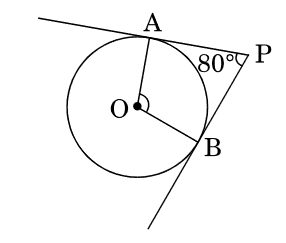
\includegraphics[width = \columnwidth]{./figs/Tangents.png}
        \caption{Tangents $PA$ and $PB$}
        \label{fig:fig1.png}
    \end{figure}
    \begin{enumerate}
        \item $100^{\degree}$
        \item $60^{\degree}$
        \item $100^{\degree}$
        \item $100^{\degree}$
    \end{enumerate}

    \item  Two concentric circles are of radii $4 cm$ and $3 cm$. Find the length of the chord of the larger circle which touches the smaller circle.

    \item  In \figref{fig:fig2.png}, a triangle $ABC$ with $\angle AOB$ is shown. Taking $AB$ as diameter, a circle has been drawn intersecting $AC$ at point $P$. Prove that the tangent drawn at point $P$ bisects $BC$. 
	        \begin{figure}[H]
 %       \centering
        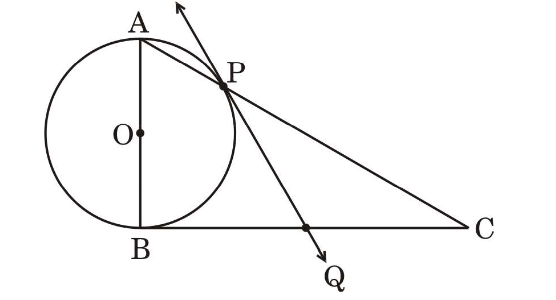
\includegraphics[width = \columnwidth]{./figs/Concentric.png}
        \caption{Concentric circles}
        \label{fig:fig2.png}
               \end{figure}
    \item  Prove that a Parallelogram circumscribing a circle is a rhombus.
     \item  In \figref{fig:fig3.png}, two circles with centres at $O$ and $O$ of radii $2r$ and $r$ respectively, touch each other internally at $A$. A chord $AB$ of the bigger circle meets the smaller circle at $C$. Show that  $C$ bisects $AB$.
    \begin{figure}[H]
        \centering
        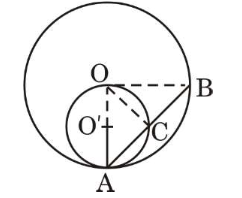
\includegraphics[width = \columnwidth]{./figs/two_circle.png}
        \caption{Two circles with center}
        \label{fig:fig3.png}
    \end{figure}  
    
    \item In \figref{fig:fig4.png}, $O$ is centre of a circle of radius $5 cm$. $PA$ and $BC$ are tangents to the circle at $A$ and $B$ respectively. If $OP = 13 cm$, then find the length of tangents $PA$ and $BC$.
\begin{figure}[H]                                                                                             \centering                                                                                                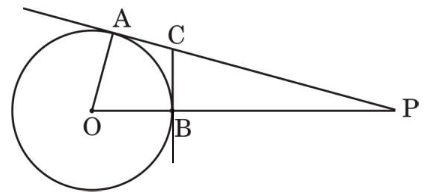
\includegraphics[width = \columnwidth]{./figs/circle_radius.png}
\caption{The center of circle radius is $5cm$} 
\label{fig:fig3.png}        
\end{figure}

    \item In two concentric circles, a chord of length $48 cm$ of the larger
circle is a tangent to the smaller circle, whose radius is $7 cm$. Find the radius of the larger circle. 
    \item At a point on the level ground, the angle of elevation of the top
of a vertical tower is found to be $\alpha$, such that $\tan \alpha =\frac{5}{12} $. On walking $192 m$ towards the tower, the angle of elevation $\beta$ is such that $\tan \beta=\frac{3}{4}$. Find the height of the tower. 
    \end{enumerate}
\end{document}

\section{2023}
\subsection{10}
%\documentclass{article}
%\usepackage{gensymb}
%\let\vec\mathbf
%\usepackage{float}
%\usepackage{graphicx}
%\newcommand\figref{Fig.~\ref}
%\graphicspath{{./Documents}}
%\begin{document}
\begin{enumerate}
	\item In the given figure \figref{fig:circle1}, $ PQ $ is tangent to the circle centred at $ \vec{O} $. If $ \angle{AOB} = 95{\degree} $, then measure of $ \angle{ABQ} $ will be
	\begin{figure}[H]
		\centering
		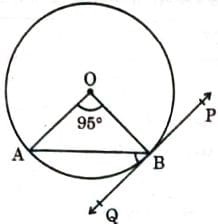
\includegraphics[width=\columnwidth]{figs/fig1.jpg}
		\caption{}
		\label{fig:circle1}
	\end{figure}
		\begin{enumerate}
			\item $ 47.5{\degree} $
			\item $ 42.5{\degree} $
			\item $ 85{\degree} $
			\item $ 95{\degree} $
		\end{enumerate}
	\item
		\begin{enumerate}
			\item In the given figure \figref{fig:circle2}, two tangents $ TP $ and $ TQ $ are drawn to be a circle with centre $ \vec{O} $ from an external point $ \vec{T} $. Prove that $ \angle{PTQ} = 2\angle{OPQ} $.
		\begin{figure}[H]
			\centering
			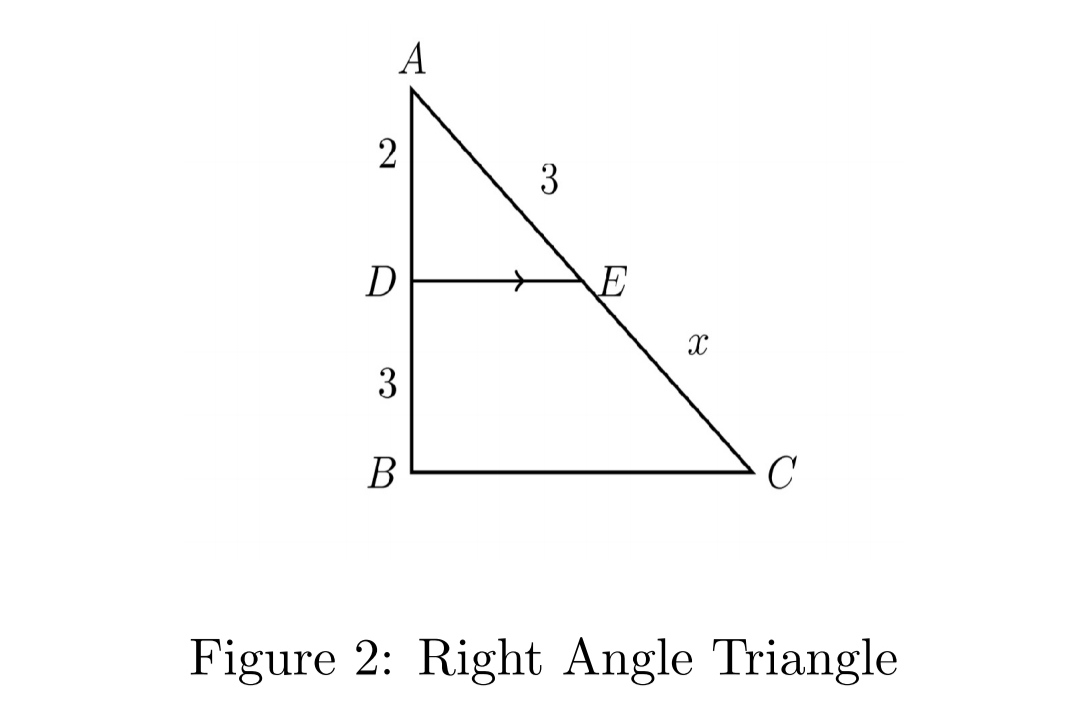
\includegraphics[width=\columnwidth]{figs/fig2.jpg}
			\caption{}
			\label{fig:circle2}
		\end{figure}
	\item In the given figure \figref{fig:circle3}, a circle is inscribed in a quadrilateral $ ABCD $ in which $ \angle{B} = 90{\degree} $. If $ AD = 17 cm, AB = 20 cm $ and $ DS = 3cm $, then find the radius of the circle.
		\begin{figure}[H]
			\centering 
			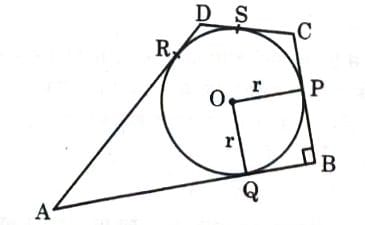
\includegraphics[width=\columnwidth]{figs/fig3.jpg}
			\caption{}
			\label{fig:circle3}
		\end{figure}
		\end{enumerate}
	\item The discus throw is an event in which an athlete attempts to throw a discus. The athlete spins anti-clockwise around one and a half times through a cicrle as shown in \figref{fig:tangentline} below, then releases the throw. When released, the discus travels along tangent to the circular spin orbit.
		\begin{figure}[H]
			\centering
			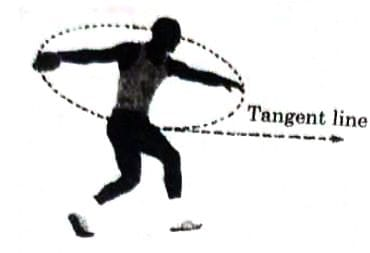
\includegraphics[width=\columnwidth]{figs/fig4.jpg}
			\caption{}
			\label{fig:tangentline}
		\end{figure}
		In the given figure \figref{fig:circle5}, $ AB $ is one such tangent to a circle of radius 75 cm. Point $ \vec{O} $ is centre of the circle and $ \angle{ABO} = 30{\degree} . PQ $ is parallel to $ OA $.
		\begin{figure}[H]
			\centering
			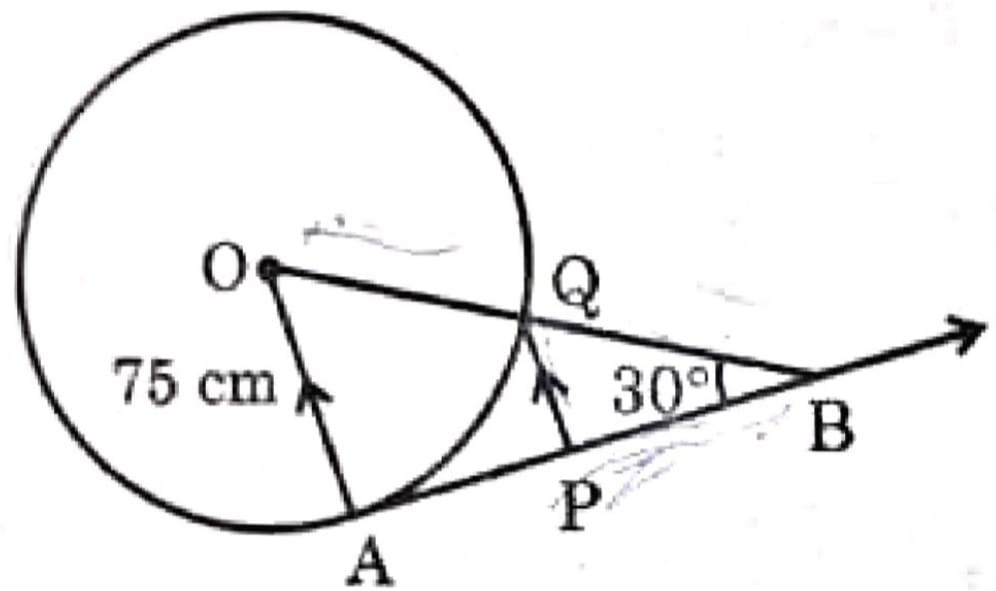
\includegraphics[width=\columnwidth]{figs/fig5.jpg}
			\caption{}
			\label{fig:circle5}
		\end{figure}
		Based on above information :
		\begin{enumerate}
			\item find the length of $ AB $.
			\item find the length of $ OB $.
			\item find the length of $ AP $.
			\item find the length of $ PQ $.
		\end{enumerate}
	\item In the given figure \figref{fig:circle6}, the quadrilateral $ PQRS $ circumscribes a circle. Here $ PA + CS $ is equal to :
		\begin{figure}[H]
			\centering
			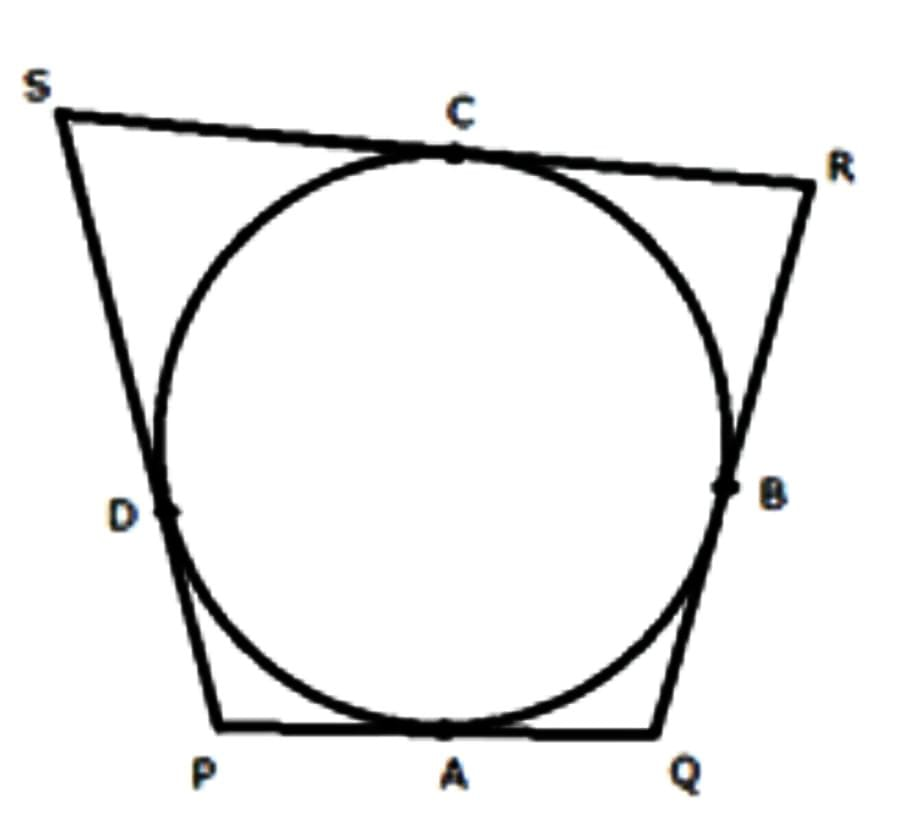
\includegraphics[width=\columnwidth]{figs/fig6.jpg}
			\caption{}
			\label{fig:circle6}
		\end{figure}
		\begin{enumerate}
			\item $ QR $
			\item $ PR $
			\item $ PS $
			\item $ PQ $
		\end{enumerate}
	\item In the given figure \figref{fig:circle7}, $ \vec{O} $ is the centre of the circle. $ AB $ and $ AC $ are tangents drawn to the circle from point $ \vec{A} $. If $ \angle{BAC} = 65{\degree} $, then find the measure of $ \angle{BOC} $.
		\begin{figure}[H]
			\centering
			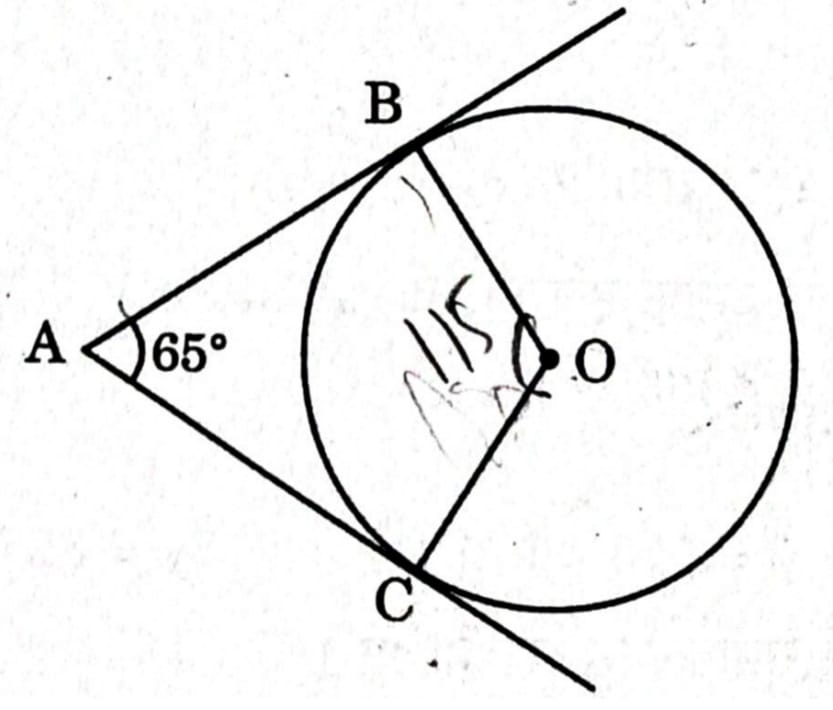
\includegraphics[width=\columnwidth]{figs/fig7.jpg}
			\caption{}
			\label{fig:circle7}
		\end{figure}
	\item In the given figure \figref{fig:circle8}, $ \vec{O} $ is the centre of the circle and $ QPR $ is the tangent to it at $ \vec{P} $. Prove that $ \angle{QAP} + \angle{APR} = 90{\degree} $.			
		\begin{figure}[H]
			\centering
			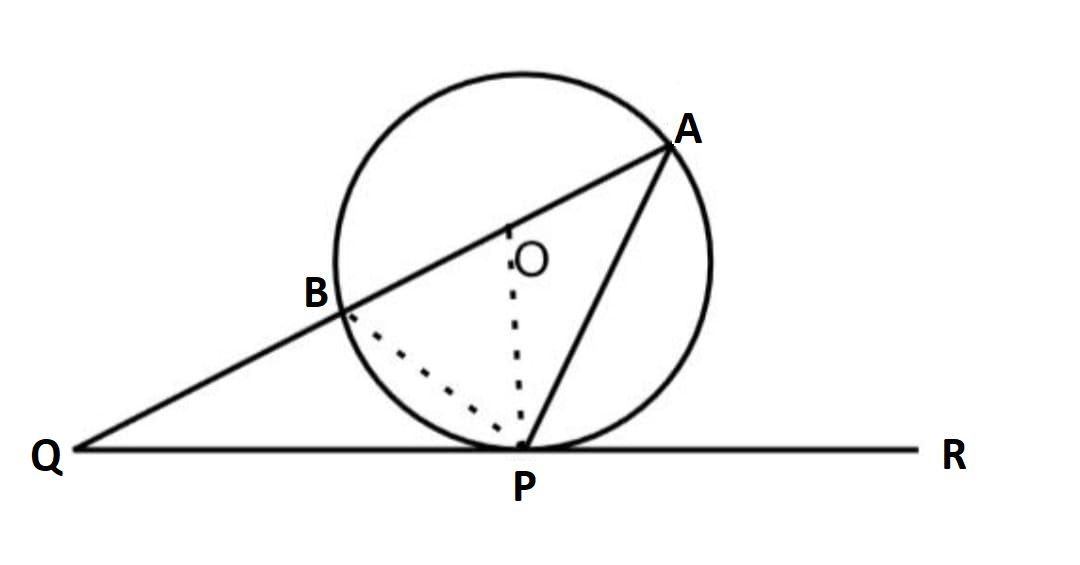
\includegraphics[width=\columnwidth]{figs/fig8.jpg}
			\caption{}
			\label{fig:circle8}
		\end{figure}
	\item In the given figure \figref{fig:circle9}, $ TA $ is a tangent to the circle with centre $ \vec{O} $ such that $ OT = 4 cm , \angle{OTA} = 30{\degree} $, then length of $ TA $ is :
		\begin{figure}[H]
			\centering
			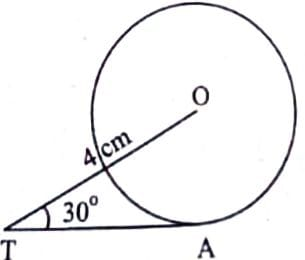
\includegraphics[width=\columnwidth]{figs/fig9.jpg}
			\caption{}
			\label{fig:circle9}
		\end{figure}
		\begin{enumerate}
			\item $ 2\sqrt{3} cm $
			\item $ 2 cm $
			\item $ 2\sqrt{2} cm $
			\item $ \sqrt{3} cm $
		\end{enumerate}
	\item In the given figure \figref{fig:circle10}, $ PT $ is a tangent at $ \vec{T} $ to the circle with centre $ \vec{O} $. If $ \angle{TPO} = 25{\degree} $, then $ x $ is equal to : 	
		\begin{figure}[H]
			\centering
			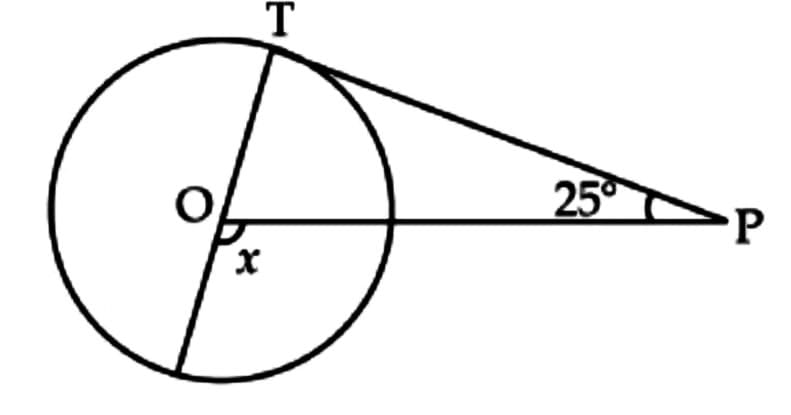
\includegraphics[width=\columnwidth]{figs/fig10.jpg}
			\caption{}
			\label{fig:circle10}
		\end{figure}
		\begin{enumerate}
			\item $ 25{\degree} $
			\item $ 65{\degree} $
			\item $ 90{\degree} $
			\item $ 115{\degree} $
		\end{enumerate}
	\item Two concentric circles are of radii 5 cm and 3 cm. Find the length of the chord of the larger circle which touches the smaller circle.
\end{enumerate}
%\end{document}

\section{2022}
\begin{enumerate}[label=\thesection.\arabic*.,ref=\thesection.\theenumi]
\numberwithin{equation}{enumi}
\numberwithin{figure}{enumi}
\numberwithin{table}{enumi}

	\item Draw a circle of radius 2.5 cm. Take a point $\vec{P}$ outside the circle at a distance of 7 cm from the center. Then construct a pair of tangents to the circle from point $\vec{P}$.

	\item Write the steps of construction for constructing a pair of tangents to a circle of radius 4 cm from a point $\vec{P}$, at a distance of 7 cm from its center $\vec{O}$.

	\item In Figure \ref{fig:tan1}, there are two concentric circles with centre $\vec{O}$. If $ARC$ and $AQB$ are tangents to the smaller circle  from the point $\vec{A}$ lying on the larger circle, find the length of $AC$, if $AQ$ = 5 cm.
		\begin{figure}[H]
			\centering
			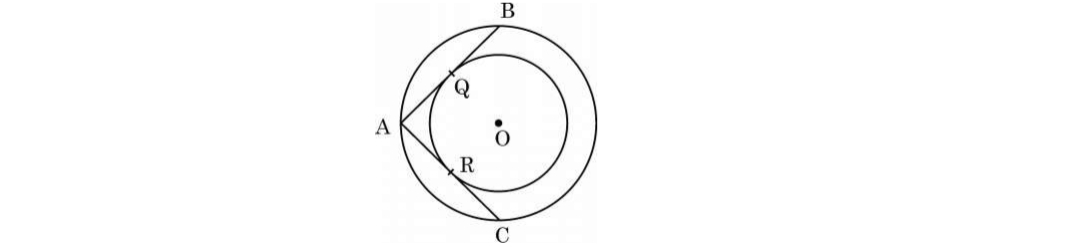
\includegraphics[width=\columnwidth]{figs/tan}
			\caption{Two concentric circles with $\vec{O}$ as centre}
			\label{fig:tan1}
		\end{figure}
	
	\item In Figure \ref{fig:cir1}, if a circle touches the side $QR$ of $\Delta PQR$ at $\vec{S}$ and extended sides $PQ$ and $PR$ at $\vec{M}$ and $\vec{N}$, respectively,
		\begin{figure}[H]
			\centering
			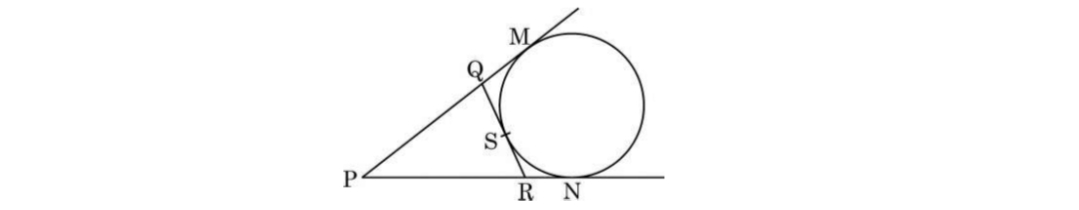
\includegraphics[width=\columnwidth]{figs/cir}
				\caption{Two tangents are drawn from point $\vec{P}$ to the circle}
				\label{fig:cir1}
		\end{figure}
		prove that $PM=\dfrac{1}{2}(PQ+QR+PR)$

	\item In Figure \ref{fig:tri1}, a triangle $ABC$ is drawn to circumscribe a circle of radius 4 cm such that the segments $BD$ and $DC$ into which $BC$ is divided by the point of contact $\vec{D}$ are of lengths 6 cm and 8 cm respectively. If the area of $\Delta ABC$ is 84 $cm^2$, find the lengths of sides $AB$ and $AC$.
		\begin{figure}[H]
			\centering
			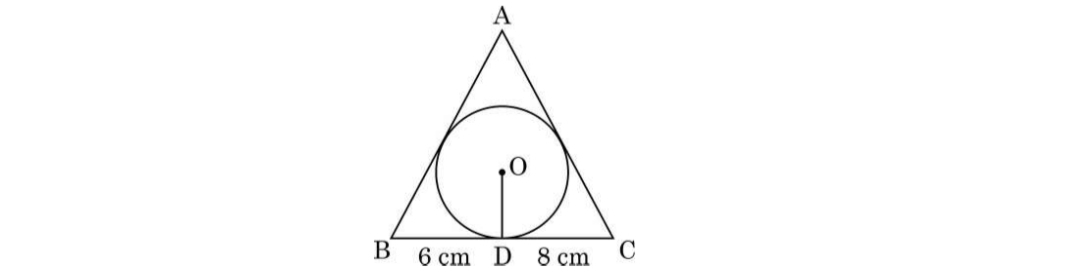
\includegraphics[width=\columnwidth]{figs/tri}
				\caption{Circle with $\vec{O}$ as center circumscribed in triangle $ABC$}
				\label{fig:tri1}
		\end{figure}

	\item In Figure \ref{fig:sq1}, $PQ$ and $PR$ are tangents to the circle centered at $\vec{O}$. If $\angle OPR=45\degree$, then prove that $ORPQ$ is a square.
		\begin{figure}[H]
			\centering
			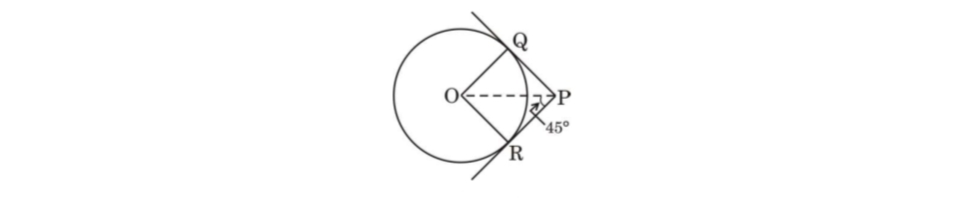
\includegraphics[width=\columnwidth]{figs/sq}
			\caption{Two tangents drawn from point $\vec{P}$ to a circle whose centre is $\vec{O}$}
			\label{fig:sq1}
		\end{figure}

	\item In Figure \ref{fig:sct1}, $\vec{O}$ is the centre of a circle of radius 5 cm. $PA$ and $BC$ are tangents to the circle at $\vec{A}$ and $\vec{B}$ respectively. If $OP$ is 13 cm, then find the length of tangents $PA$ and $BC$.
		\begin{figure}[H]
			\centering
			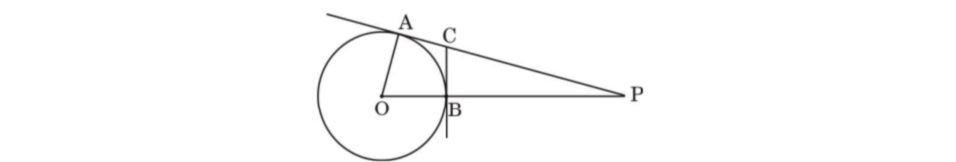
\includegraphics[width=\columnwidth]{figs/sct}
			\caption{Two tangents drawn from point $\vec{C}$ to a circle whose centre is $\vec{O}$}
			\label{fig:sct1}
		\end{figure}

	\item In Figure \ref{fig:ver1}, $AB$ is diameter of a circle centered at $\vec{O}$. $BC$ is tangent to the circle at $\vec{B}$. If $OP$ bisects the chord $AD$ and $\angle AOP=60\degree$, then find $m\angle C$.
		\begin{figure}[H]
			\centering
			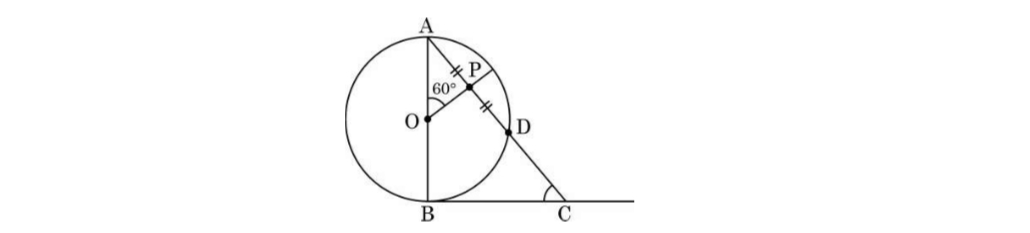
\includegraphics[width=\columnwidth]{figs/ver}
			\caption{Tangent $BC$ is drawn from point $\vec{C}$ to a circle whose centre is $\vec{O}$}
			\label{fig:ver1}
		\end{figure}

	\item In Figure \ref{fig:hor1}, $XAY$ is a tangent to the circle centered at $\vec{O}$. If $\angle ABO=60\degree$,then find $m\angle BAY$ and $m\angle AOB$.
		\begin{figure}
			\centering
			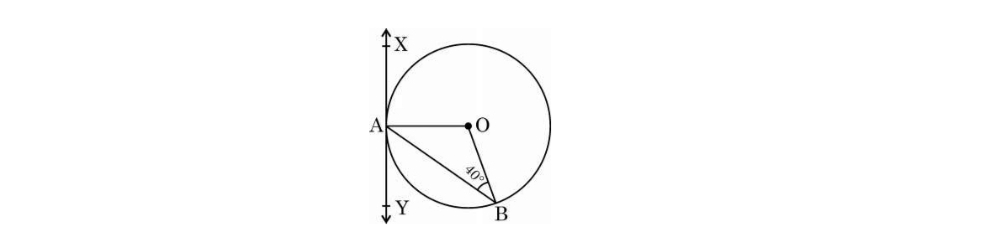
\includegraphics[width=\columnwidth]{figs/hor}
			\caption{The line $XAY$ is tangent to the circle centered at $\vec{O}$}
			\label{fig:hor1}
		\end{figure}

	\item Two concentric circles are of radii 4cm and 3 cm. Find the length of the chord of the larger circle which touches the smaller circle.

	\item In Figure \ref{fig:sl1}, a triangle $ABC$ with $\angle B=90\degree$ is shown. Taking $AB$ as diameter, a circle has been drawn intersecting $AC$ at point $\vec{P}$. Prove that the tangent drawn at point $\vec{P}$ bisects $BC$.
		\begin{figure}[H]
			\centering
			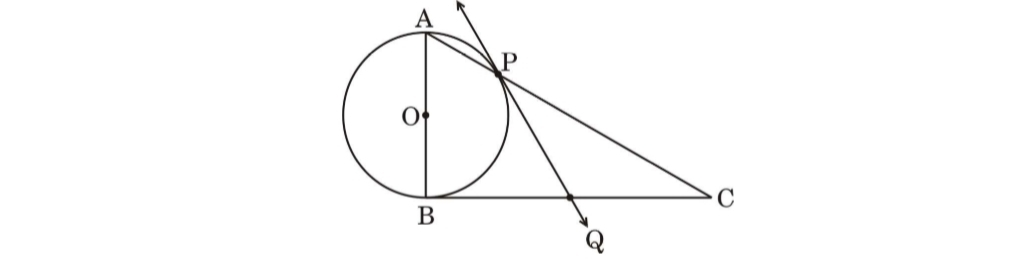
\includegraphics[width=\columnwidth]{figs/sl}
			\caption{$PQ$ is tangent to the circle centered at $\vec{O}$. $AB$ is the diameter and $\angle B=90\degree$}
			\label{fig:sl1}
		\end{figure}
\item Find the equation of tangent to the curve $y = x^2 + 4x + 1$ at the point $(3,22)$.
\end{enumerate}

\section{2021}
\subsection{10}
\documentclass{article}
\usepackage{enumitem}
\usepackage{graphicx}
%\graphicspath{{figs/}}
\usepackage{amsmath}
\usepackage{amsfonts}
\usepackage{float}
\usepackage{gensymb}
\let\vec\mathbf
\begin{document}
\title{Circles-10}
\begin{enumerate}
	\item A quadrilateral $ABCD$ is drawn to circumscribe a circle (see Figure-1). Prove that $AB + CD = AD + BC$.
	\begin{figure}[!htb]
		\centering
			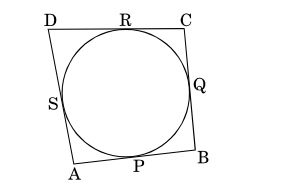
\includegraphics[width=\columnwidth]{figs/circ-1.png}
		
		\caption{}
		\label{fig:circ-1}
	\end{figure}
	\item Draw a pair of tangents to a circle of radius $4 cm$ which are inclined to each other at an angle of 45\degree.	
	\item A point $\vec{T}$ is $13 cm$ away from the centre of a circle. The length of the tangent drawn from $\vec{T}$ to the circle is $12 cm$. Find the radius of the circle.
	\item Two tangents $TP$ and $PQ$ are drawn to a circle with centre $\vec{O}$ from an external point $\vec{T}$. Prove that $\angle PTQ = 2 \angle OPQ$.
	\item $PQ$ is a tangent to a circle with centre $\vec{O}$ at the point $\vec{P}$ on the circle. If $\triangle OPQ$ is an isosceles triangle, then find $\angle OQP$.
	\item Two concentric circles have radii $10 cm$ and $6 cm$. Find the length of the chord of the larger circle which touches the smaller circle.
	\item If tangents $PA$ and $PB$ from an external point $\vec{P}$ to a circle with centre $\vec{O}$ are inclined to each other at an angle of 70\degree, then find $\angle POA$.
	\item $ABC$ is right triangle, right-angled at $\vec{B}$ with $BC = 6 cm$ and $AB = 8 cm$. A circle with centre $\vec{O}$ and radius $r$ cm has been inscribed in $\triangle ABC$ as shown in the figure. Find the value of $r$.
		\begin{figure}[H]
			\centering
			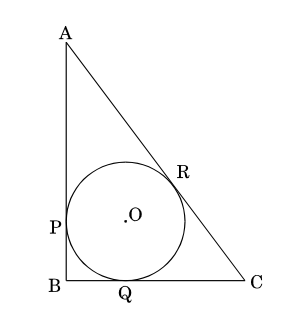
\includegraphics[width=\columnwidth]{figs/circ-2.png}
			\caption{}
			\label{fig:circ-2}
		\end{figure}
	\item Draw a circle of radius $5 cm$. From a point $8 cm$ away from its centre, construct a pair of tangents to the circle.
	\item In the given figure, $PT$ and $PS$ are tangents to a circle with centre $\vec{O}$, from a point $\vec{P}$, such that $PT = 4 cm$ and $\angle TPS = 60$\degree. Find the length of the chord $TS$. Also, find the radius of the circle.
		\begin{figure}[H]
			\centering
			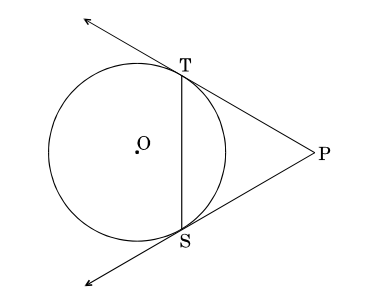
\includegraphics[width=\columnwidth]{figs/circ-3.png}
			\caption{}
			\label{fig:circ-3}
		\end{figure}
	\item \begin{enumerate}[label=(\alph*)]
			\item In a right triangle $ABC$, right-angled at $\vec{B}$, $BC = 6 cm$ and $AB = 8 cm$. A circle is inscribed in the $\triangle ABC$. Find the radius of the incircle.
			\item Two circles touch externally at $\vec{P}$ and $AB$ is a common tangent, touching one circle at $\vec{A}$ and the other at $\vec{B}$. Find the measure of $\angle APB$.
		\end{enumerate}
	\item From an external point $\vec{P}$, tangents $PQ$ and $PR$ are drawn to a circle with centre $\vec{O}$, touching the circle at $\vec{Q}$ and $\vec{R}$. If $\angle QOR = 140$\degree, find the measure of $\angle QPR$.
	\item A circle touches all the sides of a quadrilateral $ABCD$. Prove that $AB + CD = DA + BC$.
	\item Write the steps of construction of a circle of diameter $6 cm$ and drawing of a pair of tangents to the circle from a point $5 cm$ away from the centre.
\end{enumerate}
\end{document}
                                                                                

\section{2020}
\subsection{10}
\begin{enumerate}
\item In \figref{fig:circ}, from an external point $P$, two tangent $PQ$ and $PR$ are drawn to a circle of radius $4cm$ with center $O$. If$\angle{PQR}=90\degree$, then length of $PQ$ is \underline {\hspace{4cm}}.
\begin{enumerate}[label=(\alph*)]
\item $3cm$ 
\item $4cm$
\item $2cm$
\item $2{\sqrt{2}}cm$ 
\end{enumerate}
\begin{figure}[H]
\centering
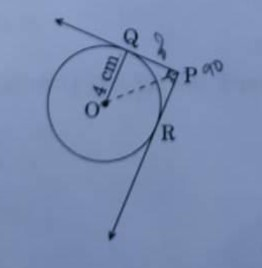
\includegraphics[width=\columnwidth]{figs/circ.jpg}
\caption{}
\label{fig:circ}
\end{figure}
\item In \figref{fig:circ2}, $PQ$ is tangent to the circe with center at $O$, at the point $B$. If$\angle AOB=100\degree$, then$\angle ABP$ is equal to\newline
\begin{enumerate}[label=(\alph*)] 
\item $50\degree$ 
\item $40\degree$ 
\item $60\degree$ 
\item $80\degree$
\end{enumerate}
\begin{figure}[H]
\centering
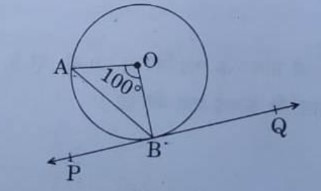
\includegraphics[width=\columnwidth]{figs/circ2.jpg}
\caption{}
\label{fig:circ2}
\end{figure}
\item In \figref{fig:circ3}, quadrilateral $ABCD$ is drawn to circumscribe a circle. Prove that\newline
$AB+CD=BC+AD$
\begin{figure}[H]
\centering
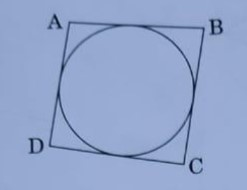
\includegraphics[width=\columnwidth]{figs/circ3.jpg}
\caption{}
\label{fig:circ3}
\end{figure}
\item In \figref{fig:circ4}, find the perimeter of $\triangle ABC$, if $AP=12cm$
\begin{figure}[H]
\centering
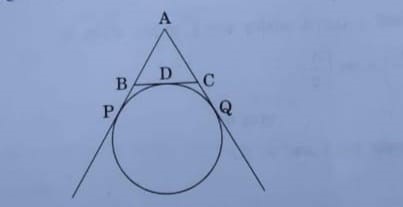
\includegraphics[width=\columnwidth]{figs/circ4.jpg}
\caption{} 
\label{fig:circ4}
\end{figure}
\end{enumerate}

\section{2019} 
\subsection{10}
\begin{enumerate}
\item $ABC$ is a right triangle in which $\angle B = 90\degree$. If $AB = 8 cm$ and $BC = 6 cm$, find the diameter of the circle inscribed in the triangle.

\item Draw two concentric circles of radii $2 cm$ and $5 cm$. Take a point $P$ on the outer circle and construct a pair of tangents $PA$ and $PB$ to the smaller circle. Measure $PA$.  


\item In  \figref{fig:Figh_3}, $PQ$ and $RS$ are two parallel tangents to a circle with centre $O$ and another tangent $AB$ with point of contact $C$ intersecting $PQ$ at $A$ and $RS$ at $B$. Prove that $\angle AOB = 90 \degree$
\begin{figure}[H]
    \centering
    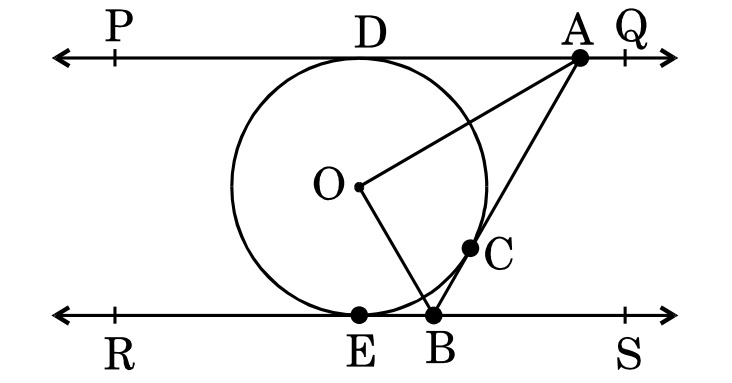
\includegraphics[width=\columnwidth]{figs/img3.jpg}
    \caption{Tangent and Circle}
    \label{fig:Figh_3}
\end{figure}
\end{enumerate}

\section{2018} 
\subsection{10}
\begin{enumerate}
	\item Prove that the lengths of tangents drawn from an external point to a circle are equal.
\end{enumerate}






\chapter{Intersection of Conics}
\section{2022}
\begin{enumerate}[label=\thesection.\arabic*.,ref=\thesection.\theenumi]
\numberwithin{equation}{enumi}
\numberwithin{figure}{enumi}
\numberwithin{table}{enumi}
\item Using integration, find the area of the region enclosed by the curve $ y=x^2 $, the x-axis and the ordinates $x=-2$ \text { and } $x=1$.

\item Using integration, find the area of the region enclosed by line $y=\sqrt{3}x$ semi-circle $y=\sqrt{4-x^2}$ and x-axis in first quadrant.

\item Using integration, find the area of the smaller region enclosed by the curve ${4x^2 + 4y^2} = 9$ and the line $2x + 2y =3$.

\item If the area of the regin bounded by the curve $y^2 = 4ax$ and the line $x = 4a$ is $\dfrac{256}{3}$\hspace{0.2cm} sq. units, then using integration, find the value of a, where $a>0$.

\item Find the area of the region enclosed by the curves $y^2=x$, $x=\dfrac{1}{4}$,  $y=0$ and $x=1$, using integration.

\item If the area of the region bounded bythe line $y=mx$ and the curve $x^2=y$ is $\dfrac{32}{3}$\hspace{0.2cm}sq. units, then find the positive value of m, using integration.

\item If the area between the curves $x = y^2$ and $x = 4$ is divided into two equal parts by the line $x = a$, then find the value of a, using integration.

\item Find the area bounded by the ellipse $x^2+4y^2=16$ and the ordinates $x=0$ and $x=2$, using integration.

\item Find the area of the region $\{(x,y) : x^2 \leq y \leq x\}$, using integration

\end{enumerate}

\section{2021}
\subsection{12}
  \begin{enumerate}
        
\item The point at which the normal to the curve 
\begin{align}
    y = x+\frac{1}{x}, x>0 
\end{align}
 is perpendicular to the line
 \begin{align}
     3x-4y-7 = 0 
 \end{align}
\begin{enumerate}
    \item $\brak{2,\frac{5}{2}}$   \item $\brak{\pm2,\frac{5}{2}}$  

         \item $\brak{-\frac{1}{2},\frac{5}{2}}$    \item $\brak{\frac{1}{2},\frac{5}{2}}$
\end{enumerate}
         
         \item The points on the curve
         \begin{align}
             \frac{x^2}{9} +\frac{y^2}{16} = 1
         \end{align}
         at which the tangents are parallel to $y$-axis are:
         \begin{enumerate}
             \item $\brak{0,\pm4}$   \item $\brak{\pm4,0}$  

         \item  $\brak{\pm3,0}$   \item $\brak{0,\pm3}$
         \end{enumerate}
           
         \item For which value of m is the line
         \begin{align}
            y = mx + 1 
         \end{align}a tangent to the curve 
        \begin{align}
            y^2 = 4x 
        \end{align}
        \begin{enumerate}
            \item  $\frac{1}{2}$  \item $1$

         \item 2  \item 3
        \end{enumerate}
    \end{enumerate}


\section{2019}
\subsection{12}
\begin{enumerate}
\item Using method of integration, find the area of the region enclosed between two circles ${x^2+y^2=4}$ and $\brak{x-2}^2+{y^2}=4$.

\item Find the equation of the normal to the curve ${x}^2 = 4y$ which passes through the point $\myvec{-1,4}$.

\item Find the point on the curve ${y}^2 = 4x$, which is nearest to the point $\myvec{2,-8}$.
\end{enumerate} 

\item Find the area of the region bounded by the curves $\brak{x-1}^{2} +y^{2} = 1$ and $ x^{2}+y^{2}  = 1$ using integration.

\item Find the area of the region 
\begin{align*}
    \cbrak{(x,y):0\leq y \leq x^{2},0 \leq y \leq x +2 , -1 \leq x \leq 3}.
\end{align*}

\item Find the area of the region bounded by the curves  
\begin{align*}
\brak{x-1}^2 +y^2=1 \\  x^2+y^2=1
\end{align*}
using integration.

\item Find the equations of the tangent and the normal to the curve 
\begin{align*}
y=\dfrac{x-7}{(x-2)(x-3)}    
\end{align*}
at the point where it cuts the x-axis.
\end{enumerate} 







\chapter{Probability}
\section{2021}
\subsection{10}

\begin{enumerate}
\item During the lockdown period,many families got bored of watching TV all the time.Out of these families, one family of 6 members decided to play a card game.17 cards numbered 1,2,3,4,..,17 are put in a box and mixed thoroughly.One card is drawn by one member at random and other family members bet for the chances of drawing the number either prime,odd or even etc.
\begin{figure}[H]
\centering
	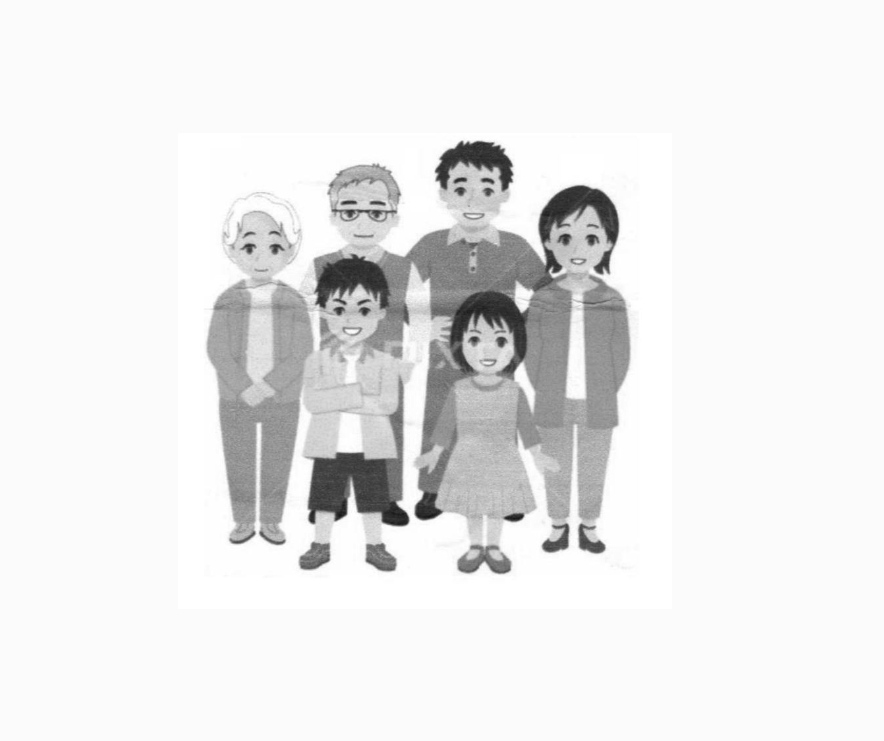
\includegraphics[width=\columnwidth]{figs/satish.jpg}                                                                                              
\caption{Family of six}
\label{fig:satish.jpg}                                                                                                                      \end{figure}
Based on the above,answer the following questions:
\begin{enumerate}                                                                                                                                       \item The first member of the family draws a card at random and another member bets that it is an even prime number.What is the probability of his winning the bet?                                                                                                                           \begin{enumerate}
        \item $\frac{2}{17}$
        \item $\frac{3}{17}$
        \item $\frac{1}{17}$
        \item $\frac{4}{17}$
\end{enumerate}
       \item The second member of the family draws a card at random and some other
member bets that it is an even number. What is the probability of his winning
the bet ?
\begin{enumerate}
        \item $\frac{7}{17}$
        \item $\frac{8}{17}$
        \item $\frac{9}{17}$
        \item $\frac{10}{17}$
\end{enumerate}
      \item What is the probability that the number on the card drawn at random is
divisible by 5 ?
\begin{enumerate}
        \item $\frac{5}{17}$
        \item $\frac{4}{17}$
        \item $\frac{3}{17}$
        \item $\frac{2}{17}$
\end{enumerate}
      \item What is the probability that the number on the card drawn at random is a
multiple of 3 ?
\begin{enumerate}
        \item $\frac{5}{17}$
        \item $\frac{6}{17}$
        \item $\frac{7}{17}$
        \item $\frac{8}{17}$
\end{enumerate}   
\end{enumerate}                                                                                                                                       
\item 
\item Two different coins are tossed simultaneously. Write all the possible outcomes.                                                                   
\item A die is thrown once. Write the probability of getting a number less than $7$.

\item  If the probability of occurrence of event E,\pr{E}=0.99, what is the probability of non-occurrence of the event E,\pr {not E}?                   \item \begin{enumerate}
\item A bag contains 5 white balls and 7 red balls.A ball is drawn at random from the bag.What is the probability that it is either a white or a red ball?
\item Two coins are tossed together once.What is the probability of getting at least one head?
\end{enumerate}
\item Cards marked with numbers $1$,$2$,$3$,$4$, ..., $100$ are placed in a bag and mixed together throughly. A card is randomly drawn from the bag.Find the probability that the numbers on the card is                             \begin{enumerate}                                                                                                                     \item an even number,
\item a $2$-digit number,
\item a perfect square.                                         
\end{enumerate}
\item \begin{enumerate}
\item How many outcomes are possible when three dice are thrown together?
\item if \pr{E}=0.015, then find \pr{not E}.
\end{enumerate}
\item  During summer break, Harish wanted to play with his friends but it was too hot outside, so he decided to play some indoor game with his friends. He collects $20$ identical Icards and writes the numbers $1$ to $20$ on them (one number on one card). He puts them in a box. He and his friends make a bet for the chances of drawing various cards out of the box. Ench was given a chance to tell the probability of picking one card out of the box.

Based on the above,answer the following questions:
\begin{enumerate}                                                                                                                                 \item The probability that the number on the card drawn is an odd prime number,is
\begin{enumerate}                           

          \item $\frac{3}{5}$
          \item $\frac{2}{5}$
          \item $\frac{9}{20}$                      
          \item $\frac{7}{20}$                                               \end{enumerate}
\item The probability that the number on the card drawn is a composite number is
\begin{enumerate}
        \item $\frac{11}{20}$                     
	\item $\frac{3}{5}$                       
	\item $\frac{4}{5}$                     
	\item $\frac{1}{2}$
\end{enumerate}
\item The probability that the number on the card drawn is a multiple of $3$,$6$ and $9$ is
\begin{enumerate}               
	\item $\frac{1}{20}$                      
	\item $\frac{1}{20}$                      
	\item $\frac{3}{20}$                      
	\item $0$
\end{enumerate}
\item The probability that the number on the card drawn is a multiple of $3$ and $7$is
\begin{enumerate}                 
	\item $\frac{3}{10}$                      
	\item $\frac{1}{10}$                      
	\item $0$
        \item $\frac{2}{5}$               
\end{enumerate}                                                              \item If all cards having odd numbers written on them are removed from the box and then one card is drawn from the remaining cards, the probability of getting a card having a prime number is
\begin{enumerate}                
	\item $\frac{1}{20}$
	\item $\frac{1}{10}$                      
        \item $0$ 
        \item $\frac{1}{5}$               
\end{enumerate}
\end{enumerate}
\item \begin{enumerate}
\item In a single throw of a pair of dice,find the probability that both dice have the same number.
\item A card is drawn from a well-shuffled pack of $52$ cards.Find the probability that it is not an ace.
\end{enumerate}
\end{enumerate}

\subsection{12}
\documentclass{article}
\usepackage{siunitx}
\usepackage{setspace}
\usepackage{gensymb}          
\usepackage{xcolor}
\usepackage{caption}
%\usepackage{subcaption}
%\doublespacing               
\singlespacing   
\usepackage[none]{hyphenat}   
\usepackage{amssymb} 
%\usepackage{relsize} 
\usepackage[cmex10]{amsmath}  
\usepackage{mathtools}      
\usepackage{amsmath}   
\usepackage{commath}  
%\usepackage{amsthm}    
%\interdisplaylinepenalty=2500 
%\savesymbol{iint}   
%\usepackage{txfonts}
%\restoresymbol{TXF}{iint}  
%\usepackage{wasysym}    
\usepackage{amsthm}   
\usepackage{mathrsfs}
\usepackage{txfonts}
\let\vec\mathbf{}
%\usepackage{stfloats}
\usepackage{float}
\usepackage{cite}
\usepackage{cases}
\usepackage{subfig}
%\usepackage{xtab}
\usepackage{longtable}
\usepackage{multirow}
%\usepackage{algorithm}
\usepackage{amssymb}
%\usepackage{algpseudocode}
\usepackage{enumitem}
\usepackage{mathtools}
%\usepackage{eenrc}
%\usepackage[framemethod=tikz]{mdframed}
\usepackage{listings}
\usepackage{listings}         
\usepackage[latin1]{inputenc}   
%% \usepackage{color}        
%% \usepackage{lscape}       
\usepackage{titling}                 
%\usepackage{fulbigskip}   
\usepackage{tikz}      
\usepackage{graphicx}
\graphicspath{{/Internal storage/Download/FWC
}}
\usepackage{atbegshi}
%http://ctan.org/pkg/atbegshi
\AtBeginDocument{\AtBeginShipoutNext{\AtBeginShipoutDiscard}}
%
\begin{document}
\begin{center}
\title{\textbf{CBSE - 12} \\ {PROBABILITY}}

\date{}
\maketitle
\end{center}
\begin{enumerate}
    \item The probability of solving a specific question independently by $A$ and $B$ are $\frac{1}{3}$ and $\frac{1}{5}$ respectively.If both try to solve the question independently, the probability that the question is solved is
    \begin{enumerate}
        \item $\frac{7}{15}$
        \item $\frac{8}{15}$
        \item $\frac{2}{15}$
        \item $\frac{14}{15}$
    \end{enumerate}
   
    \item From a pack of 52 cards, 3 cards are drawn at random (without replacement).The probability that they are two red cards and one black card is$\underline{\hspace{2cm}}$.
    \item A bag contains 19 tickets, numbered 1 to 19. A ticket is drawn at random and then another ticket is drawn without replacing the first one in the bag. Find the probability distribution of the number of even numbers on the ticket.
   
    \item Find the probability distribution of the number of successes in two tosses of a die, when a success is defined as "number greater than 5".
    \item A bag contains 5 red and 4 black balls, a second bag contains 3 red and 6 black balls. One of the two bags is selected at random and two balls are drawn at random (without replacement), both of which are found to be red. Find the probability that these two balls are drawn from the second bag.
   
    
    \item An unbiased die is thrown. What is the probability of getting an odd number or a multiple of 3 ?\begin{enumerate}
        \item $\frac{3}{4}$
        \item $\frac{1}{2}$
        \item $\frac{2}{3}$
        \item $\frac{1}{3}$
    \end{enumerate}
    \item A card is drawn from an ordinary pack of 52 cards and a gambler bets that it 
is a heart or a king card. What are the odds against his winning this bet ?
\begin{enumerate}
    \item 4 : 9
    \item 1 : 4
    \item 4 : 1
    \item 9 : 4
\end{enumerate}
\item In a lottery of 25 tickets, numbered 1 to 25, two tickets are drawn simultaneously. Find the probability that none of the tickets has prime number.
\item If $E_1$ and $E_2$ are two events, where $E_1$ is a subset of $E_2$, then evaluate $P(E_2 \mid E_1)$.
\item Two dice are thrown simultaneously. Find the probability of getting a multiple of 3 on one dice and a multiple of 2 on the other dice.

 \item An urn contains 4 white, 7 green and 9 blue balls. If two balls are drawn at random, find the probability that the drawn balls are of the same colour. 
\end{enumerate}

\end{document}

\section{2023}
\subsection{10}
\begin{enumerate}
	\item Probability of happining of an event is denoted by $p$ and probability of non-happening of the event is denoted by $q$. Relation between $p$ and $q$ is
                        \begin{enumerate}
                                \item $p$+$q$=1
                                \item $p$=1, $q$=1
                                \item $p$=$q$-1
                                \item $p$+$q$+1=0
                        \end{enumerate}
			
        \item A girl calculates that the probability of her winning the first prize in a lottery is 0.08. If 6000 tickets are sold, how many tickets has she bought ?
                        \begin{enumerate}
                                \item  40
                                \item  240
                                \item  480
                                \item  750

                        \end{enumerate}
        \item In a group of 20 people, 5 can't swim. If one person is selected at random, then the probability that he/sh can swim, is
                        \begin{enumerate}
                                \item $ \frac {3} {4} $
                                \item $ \frac {1} {3} $
                                \item 1
                                \item $ \frac {1} {4} $
                        \end{enumerate}
        \item A bag contain 4 red, 3 blue and 2 yellow balls. One ball is drawn at random from the bag. Find the probability that drawn ball is
                \begin{enumerate}
                                        \item red
                                        \item yellow
                \end{enumerate}
        \item A bag contain 100 cards numbered 1 to 100.Acard is drawn at random from the b. What is the probability that the number on the card is a perfect cube ?
                        \begin{enumerate}
                                \item $ \frac {1} {20} $
                                \item $ \frac {3} {50} $
                                \item $ \frac {1} {25} $
                                \item $ \frac {7} {100} $
                        \end{enumerate}
        \item If three coins are tossed simultaneously, what is the probability of getting a most one trail ?
                        \begin{enumerate}
                                \item $ \frac {3} {8} $
                                \item $ \frac {4} {8} $
                                \item $ \frac {5} {8} $
                                \item $ \frac {7} {8} $
                        \end{enumerate}
        \item Two dics are thrown together. The probability of getting the difference of numbers on their upper faces equals to 3 is :
                        \begin{enumerate}
                                \item $ \frac {1} {9} $
                                \item $ \frac {2} {9} $
                                \item $ \frac {1} {6} $
                                \item $ \frac {1} {12} $
                        \end{enumerate}
        \item A card is drawn at random from a well-shuffled pack of 52 cards. The probability that the card drawn is not an ace is :

                        \begin{enumerate}
                                \item $ \frac {1} {13} $
                                \item $ \frac {9} {13} $
                                \item $ \frac {4} {13} $
                                \item $ \frac {12} {13} $
                        \end{enumerate}
        \item \textbf{Assertion (A) : } The probability that a leap year has 53 Students is $ \frac {2} {7} $.\\
                \textbf{Reason (R) : } The probability that a non-leap year has 53 Sundays is $ \frac {5} {7} $.

                          \begin{enumerate}
                                  \item Both Assertion (A) and Reason (R) are true and Reason (R) is the correct explanation of Assertion (A).
                                  \item Both Assertion (A) and Reason (R) are true and Reason (R) is not the correct explanation of Assertion (A).
                                  \item Assertion (A) is true but Reason (R) is false.
                                  \item Assertion (A) is false but Reason (R) is true.
                          \end{enumerate}


\end{enumerate}

\subsection{12}
\begin{enumerate}[label=\thesection.\arabic*.,ref=\thesection.\theenumi]
\numberwithin{equation}{enumi}
\numberwithin{figure}{enumi}
\numberwithin{table}{enumi}
	
	\item If A and B are two events such that 
		\begin{align}
			\pr{A|B} = 2 \times  \pr{B|A}\pr{A} + \pr{B}  = \frac{2}{3}
		\end{align}then \pr{B}  is equal to
\begin{enumerate}
\item $\frac{2}{9}$
\item $\frac{7}{9}$
\item $\frac{4}{9}$
\item $\frac{5}{9}$
\end{enumerate}

\item
\begin{enumerate}
\item Two balls are drawn at random one by one with replacement from an urn containing equal number of red balls and green balls. Find the probability distribution of number of red balls. Also, find the mean of the random variable.
\item A and B throw a die alternately till one of them gets '6' and wins the game. Find their respective probabilities of winning, if A starts the game first.
\end{enumerate}

\item Recent studies suggest that roughly $12\%$ of the world population is left handed.
	
\begin{figure}[h!]
\centering
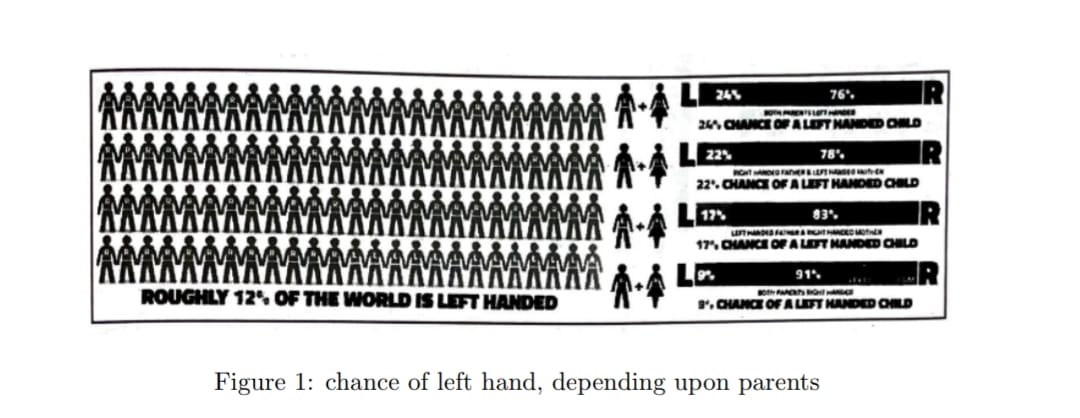
\includegraphics[width=\columnwidth]{figs/left.png}
\caption{chance of left hand, depending upon parents}
\label{fig:left.png}
\end{figure}

Depending upon the parents, the chances of having a left handed child are as follows :\\
\begin{enumerate}
\item   When both father and mother are left handed :
        Chances of left handed child is $24\%$.
\item   When father is right handed and mother is left handed :
        Chances of left handed child is $22\%$.
\item   when father is left handed and mother is right handed :
        Chances of left handed child is $17\%$.
\item   When both father nd mother are right handed :
        Chances of left handed child is $9\%$.
\end{enumerate}
Assuming that $\pr{A}=\pr{B}=\pr{C}=\pr{D}=\frac{1}{4}$ and L denotes the event that child is left handed.
Based on the above information, answer the following questions :\\
\begin{enumerate}
	\item    Find \pr{L|C}
	\item    Find \pr{\overline{L}|A}
	\item    Find \pr{A|L}
\item    Find the probability that a randomly selected child is left handed given that exactly one of the parent is left handed.
\end{enumerate}
\end{enumerate}

\section{2022}
\subsection{10}
\begin{enumerate}[label=\arabic*.,ref=\theenumi]
\item Two dice are thrown simultaneously. The probability that the sum of two numbers appearing on the top of the dice is less than $12$, is
 \begin{enumerate}
        \item $\frac{1}{36}$
        \item $\frac{35}{36}$
        \item $0$
        \item $1$
    \end{enumerate}

\item A jar contains $18$ marbles. Some are red and others are yellow. If a 
marble is drawn at random from the jar, the probability that it is red is $\frac{2}{3}$. Find the number of yellow marbles in the jar.
    \end{enumerate}

\section{2022}
\subsection{12}
\begin{enumerate}[label=\thesection.\arabic*.,ref=\thesection.\theenumi]
\numberwithin{equation}{enumi}
\numberwithin{figure}{enumi}
\numberwithin{table}{enumi}
\item Let A and B be two events such that $P(A) = \frac{5}{8}$, $P(B) = \frac{1}{2}$ and  $P(A|B) = \frac{3}{4}$. Find the value of $P(B|A)$.
\item Two balls are drawn at random from a bag containing 2 red balls and 3 blue balls, without replacement. Let the variables X denotes the number of red balls. Find the probabillity distribution of X.
\item A card from a pack of 52 playing cards is lost. From the remaining cards, 2 cards are drawn at random without replacement, and are found to be both aces. Find the probability that lost card being an ace.
\item Probabilities of A and B solving a specific problem are $\frac{2}{3}$ and $\frac{3}{5},$ respectively. If both of them try independently to solve the problem, then find the probability that the problem is  solved.
\item A pair of dice is thrown. It is given that the sum of numbers  appearing on both dice is an even number. Find the probability that the number apprearing on at least one die is 3.
\item At the start of a cricket match, a coin is tossed and the team winning the toss has the opportunity to choose to bat or bowl. such a coin is unbaised with equal probabilities of getting head and tail \figref{fig:2022/probability/coin1} .
\begin{figure}[!ht]
\centering
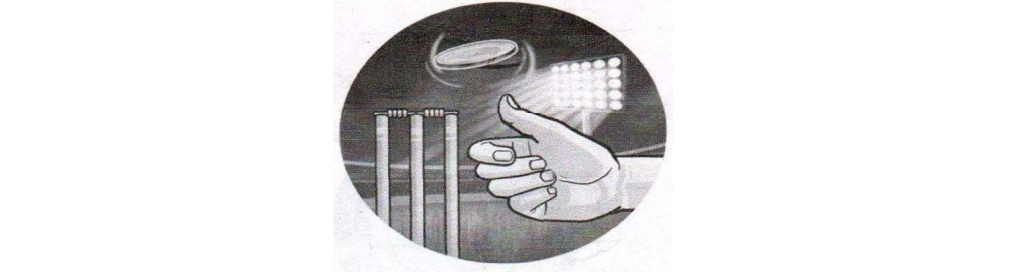
\includegraphics[width=\columnwidth]{figs/coin}
\caption{Toss before the match}
\label{fig:2022/probability/coin1}
\end{figure}
\\ Based on the above information, answer the following question:
\begin{enumerate}
\item If such a coin is tossed 2 times, then find the probability distibution of numbers of tails.
\item Find the probability of getting at least one head in three tosses of such a coin.
\end{enumerate}
\item Two cards are drawn successively with replacement from a well shuffled pack of 52 cards. Find the probability distribution of the number of spade cards.
\item A pair of dice is thrown and the sum of the numbers appearing on the dice is observed to be 7. Find the probability that the number 5 has appeared on at least one die.
\item The probability that A hits the target is $\frac{1}{3}$ and the probability that B hits it, is $\frac{2}{5}.$ If both try to hit the target independently, find the probabillity that the target is hit. 
\item A shopkeeper sells three types of flower seeds A$_1$ , A$_1$ , A$_3$. They are sold in the form of a mixture, where the proportions of these seeds are  4 : 4 : 2, respectively. The germinaton rates of the three types of seeds are $45\%,$ $60\%$ and $35\%$ respectively \figref{fig:2022/probability/flowers11}.
\begin{figure}[!ht]
\centering                                  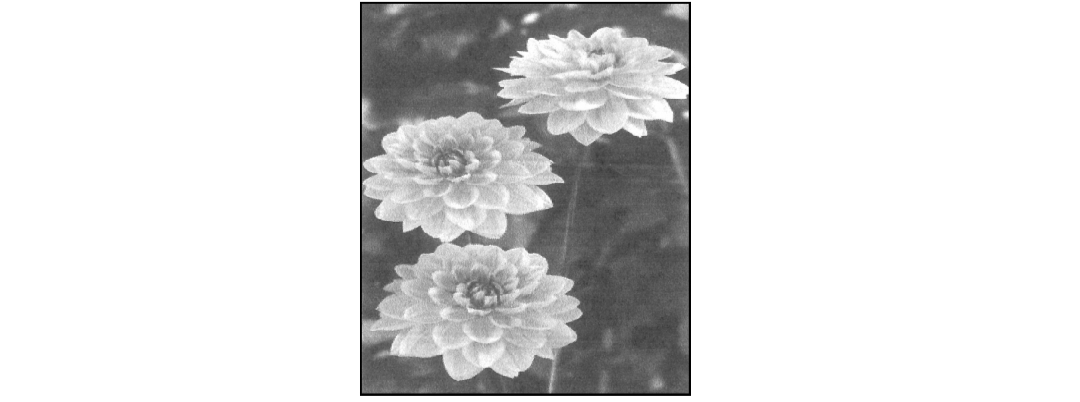
\includegraphics[width=\columnwidth]{figs/flowers}                                     
\caption{Three types of flowers}            
\label{fig:2022/probability/flowers11}                       
\end{figure}
\\ Based on  the above information :
\begin{enumerate}
\item  Calculate the probability that a randomly chosen seed will germinate.
\item  Calculate the probability  that the seed is of type $A_2$, given that a randomly choosen seed germinates.
\end{enumerate}
\item Three friends A, B and C got their photograph clicked. Find the probability that B is standing at the central position, given that A is standing at the left corner.
\item In a game of Archery, each ring of the Archery target is valued. The centremost ring is worth 10 points and rest of the rings are alloted points 9 to 1 in sequential order moving outwards.Archer A is likely to earn 10 points with a probability of 0.8 and Archer B is likely the earn 10 points with a probability of 0.9 \figref{fig:2022/probability/archery3}.
\begin{figure}[!ht]                     
\centering
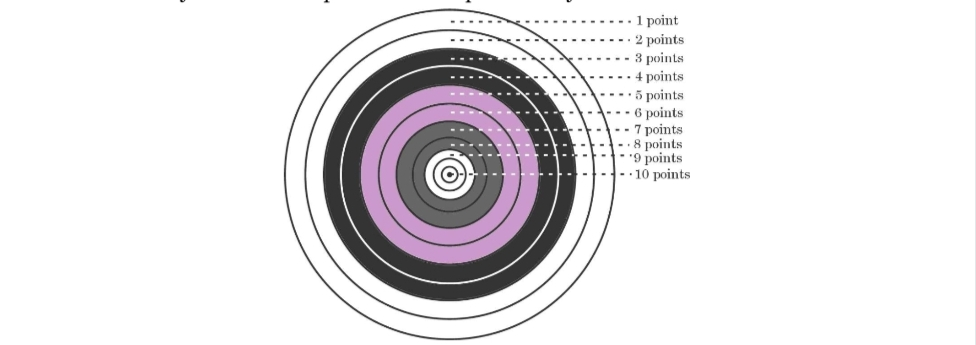
\includegraphics[width=\columnwidth]{figs/archery}
\caption{centermost ring}                   
\label{fig:2022/probability/archery3}                        
\end{figure}
\\ Based on the above innformation, answer the following questions :
\begin{enumerate}
\item exactly one of them earns 10 points .
\item both of them earn 10 point.
\end{enumerate}
\item Event A and B are such that \begin{align} P(A) = \frac{1}{2},  P(B) = \frac{7}{12}\end{align} and \begin{align} P(\bar{A}\cup \bar{B}) = \frac{1}{4} \end{align}
Find whether the events  A and B are independent or not.
\item A box $B_1$ contain 1 white ball  and 3 red balls. Another box $B_2$ contains 2 white balls and 3 red balls. If one ball is drawn at random from each of the boxes $B_1$ and $B_2$, then find the probability that the two balls drawn are of the same colour.
\item Let X be random variable which assumes values $x_1$, $x_2$, $x_3$, $x_4$  such that\begin{align} 2P(X = x_1) = 3P (X = x_2) = P ( X = x_3) = 5P (X = x_4).\end{align}
\\ Find the probability distribution of X.
\item There are two boxes, namely box-I and box-II. Box-I contains  3 red and 6 black balls. Box-II contains 5 red and 5 black balls. One of the two boxes , is selected at random and a ball is drawn at random. The ball drawn is found to be red. Find the probability that this red ball comes out from box-II.
\item In a toss of three different coins, find the probability of comming up of three heads, if it is known that at least one head comes up.
\item A laboratory blood text is $98\%$ effective  in detecting a certain disease when it is fact, present. However, the text also yeilds a false positive result for $0.4\%$ of the healthy person tested. From a large population, it is given that $0.2\%$ of the population actually has the diseases.
\\Based on the above, answer the following questtion : 
\begin{enumerate}
\item one person, from the population, is taken at random and given the test. Find the probabiliy of his getting a positive test result.
\item what is the probability that the person actually has the disease, given that his test result is positive ?
\end{enumerate}
\item Two cards are drawn from a well-shuffled pack of playing cards one-by-one with replacement. The probability that the first card is a king and the second card is a queen is 
\begin{enumerate}
\item $\frac{1}{13} + \frac{1}{13}$
\item $ \frac{1}{13} \times \frac{4}{51}$
\item $\frac{4}{52} \times \frac{3}{51}$
\item $\frac{1}{13} \times \frac{1}{13}$
\end{enumerate}
\item For two events A and B if P(A) = $\frac{4}{10}, P{B} = \frac{8}{10}$ and $P(B|A)$ = $\frac{6}{10}$ then find $P( A \cup B).$
\item Bag I contain 4 red and 3 black balls. Bag II contains 3 red and 5 black balls. One of two bags is selected at random and a ball is drawn from the bag, which if found to be red. Find the probability that the ball is drawn from bag II.
\item Two cards are drawn successively without replacement from a well-shuffled pack of 52 cards. Find the probability distribution of the number of aces and hence find its mean.
\item The probability of solving a specific question independently by A and B are $\frac{1}{3}$ and $\frac{1}{5}$ respectively . If both try to solve the question independently, the probability that the question is solved is 
\begin{enumerate}
\item $\frac{7}{15}$
\item $\frac{8}{15}$
\item $\frac{2}{15}$
\item $\frac{14}{15}$
\end{enumerate}
\item A card is picked at random from a pack of 52 playing cards. Given that the picked up card is a queen, the probability of it being a queen of spades is \underline{\hspace{1cm}}.
\item A bag contains 19 tickets, numbered 1 to 19. A ticket is drawn at random and then another ticket is drawn without replacing the first one in the bag. Find the probability distribution of the number of even numbers on the ticket.
\item Find the probability distribution of the numbers of successes in two tosses of a die, when a success is defined as number greater than 5.
\item Ten cartoons are taken at random from an automatic packing machine. The mean net weight of the ten carton is 11.8 kg and standard deviation is 0.15 kg. Does the sample mean differ significantly from the intended mean of 12 kg ?
[Given that for d.f. = 9, $t_{0.05}$ = 2.26]
\item A Coin is tossed twice. The following table\ref{tab: Number of tails} shows the probability distribution of numbers of tails:
\begin{table}[!ht]
%%%%%%%%%%%%%%%%%%%%%%%%%%%%%%%%%%%%%%%%%%%%%%%%%%%%%%%%%%%%%%%%%%%%%%
%%                                                                  %%
%%  This is the header of a LaTeX2e file exported from Gnumeric.    %%
%%                                                                  %%
%%  This file can be compiled as it stands or included in another   %%
%%  LaTeX document. The table is based on the longtable package so  %%
%%  the longtable options (headers, footers...) can be set in the   %%
%%  preamble section below (see PRAMBLE).                           %%
%%                                                                  %%
%%  To include the file in another, the following two lines must be %%
%%  in the including file:                                          %%
%%        \def\inputGnumericTable{}                                 %%
%%  at the beginning of the file and:                               %%
%%        \input{name-of-this-file.tex}                             %%
%%  where the table is to be placed. Note also that the including   %%
%%  file must use the following packages for the table to be        %%
%%  rendered correctly:                                             %%
%%    \usepackage[latin1]{inputenc}                                 %%
%%    \usepackage{color}                                            %%
%%    \usepackage{array}                                            %%
%%    \usepackage{longtable}                                        %%
%%    \usepackage{calc}                                             %%
%%    \usepackage{multirow}                                         %%
%%    \usepackage{hhline}                                           %%
%%    \usepackage{ifthen}                                           %%
%%  optionally (for landscape tables embedded in another document): %%
%%    \usepackage{lscape}                                           %%
%%                                                                  %%
%%%%%%%%%%%%%%%%%%%%%%%%%%%%%%%%%%%%%%%%%%%%%%%%%%%%%%%%%%%%%%%%%%%%%%



%%  This section checks if we are begin input into another file or  %%
%%  the file will be compiled alone. First use a macro taken from   %%
%%  the TeXbook ex 7.7 (suggestion of Han-Wen Nienhuys).            %%
\def\ifundefined#1{\expandafter\ifx\csname#1\endcsname\relax}


%%  Check for the \def token for inputed files. If it is not        %%
%%  defined, the file will be processed as a standalone and the     %%
%%  preamble will be used.                                          %%
\ifundefined{inputGnumericTable}

%%  We must be able to close or not the document at the end.        %%
	\def\gnumericTableEnd{\end{document}}


%%%%%%%%%%%%%%%%%%%%%%%%%%%%%%%%%%%%%%%%%%%%%%%%%%%%%%%%%%%%%%%%%%%%%%
%%                                                                  %%
%%  This is the PREAMBLE. Change these values to get the right      %%
%%  paper size and other niceties.                                  %%
%%                                                                  %%
%%%%%%%%%%%%%%%%%%%%%%%%%%%%%%%%%%%%%%%%%%%%%%%%%%%%%%%%%%%%%%%%%%%%%%

	\documentclass[12pt%
			  %,landscape%
                    ]{report}
       \usepackage[latin1]{inputenc}
       \usepackage{fullpage}
       \usepackage{color}
       \usepackage{array}
       \usepackage{longtable}
       \usepackage{calc}
       \usepackage{multirow}
       \usepackage{hhline}
       \usepackage{ifthen}

	\begin{document}


%%  End of the preamble for the standalone. The next section is for %%
%%  documents which are included into other LaTeX2e files.          %%
\else

%%  We are not a stand alone document. For a regular table, we will %%
%%  have no preamble and only define the closing to mean nothing.   %%
    \def\gnumericTableEnd{}

%%  If we want landscape mode in an embedded document, comment out  %%
%%  the line above and uncomment the two below. The table will      %%
%%  begin on a new page and run in landscape mode.                  %%
%       \def\gnumericTableEnd{\end{landscape}}
%       \begin{landscape}


%%  End of the else clause for this file being \input.              %%
\fi

%%%%%%%%%%%%%%%%%%%%%%%%%%%%%%%%%%%%%%%%%%%%%%%%%%%%%%%%%%%%%%%%%%%%%%
%%                                                                  %%
%%  The rest is the gnumeric table, except for the closing          %%
%%  statement. Changes below will alter the table's appearance.     %%
%%                                                                  %%
%%%%%%%%%%%%%%%%%%%%%%%%%%%%%%%%%%%%%%%%%%%%%%%%%%%%%%%%%%%%%%%%%%%%%%

\providecommand{\gnumericmathit}[1]{#1} 
%%  Uncomment the next line if you would like your numbers to be in %%
%%  italics if they are italizised in the gnumeric table.           %%
%\renewcommand{\gnumericmathit}[1]{\mathit{#1}}
\providecommand{\gnumericPB}[1]%
{\let\gnumericTemp=\\#1\let\\=\gnumericTemp\hspace{0pt}}
 \ifundefined{gnumericTableWidthDefined}
        \newlength{\gnumericTableWidth}
        \newlength{\gnumericTableWidthComplete}
        \newlength{\gnumericMultiRowLength}
        \global\def\gnumericTableWidthDefined{}
 \fi
%% The following setting protects this code from babel shorthands.  %%
 \ifthenelse{\isundefined{\languageshorthands}}{}{\languageshorthands{english}}
%%  The default table format retains the relative column widths of  %%
%%  gnumeric. They can easily be changed to c, r or l. In that case %%
%%  you may want to comment out the next line and uncomment the one %%
%%  thereafter                                                      %%
\providecommand\gnumbox{\makebox[0pt]}
%%\providecommand\gnumbox[1][]{\makebox}

%% to adjust positions in multirow situations                       %%
\setlength{\bigstrutjot}{\jot}
\setlength{\extrarowheight}{\doublerulesep}

%%  The \setlongtables command keeps column widths the same across  %%
%%  pages. Simply comment out next line for varying column widths.  %%
\setlongtables

\setlength\gnumericTableWidth{%
	53pt+%
	53pt+%
	53pt+%
	53pt+%
0pt}
\def\gumericNumCols{4}
\setlength\gnumericTableWidthComplete{\gnumericTableWidth+%
         \tabcolsep*\gumericNumCols*2+\arrayrulewidth*\gumericNumCols}
\ifthenelse{\lengthtest{\gnumericTableWidthComplete > \linewidth}}%
         {\def\gnumericScale{1*\ratio{\linewidth-%
                        \tabcolsep*\gumericNumCols*2-%
                        \arrayrulewidth*\gumericNumCols}%
{\gnumericTableWidth}}}%
{\def\gnumericScale{1}}

%%%%%%%%%%%%%%%%%%%%%%%%%%%%%%%%%%%%%%%%%%%%%%%%%%%%%%%%%%%%%%%%%%%%%%
%%                                                                  %%
%% The following are the widths of the various columns. We are      %%
%% defining them here because then they are easier to change.       %%
%% Depending on the cell formats we may use them more than once.    %%
%%                                                                  %%
%%%%%%%%%%%%%%%%%%%%%%%%%%%%%%%%%%%%%%%%%%%%%%%%%%%%%%%%%%%%%%%%%%%%%%

\ifthenelse{\isundefined{\gnumericColA}}{\newlength{\gnumericColA}}{}\settowidth{\gnumericColA}{\begin{tabular}{@{}p{53pt*\gnumericScale}@{}}x\end{tabular}}
\ifthenelse{\isundefined{\gnumericColB}}{\newlength{\gnumericColB}}{}\settowidth{\gnumericColB}{\begin{tabular}{@{}p{53pt*\gnumericScale}@{}}x\end{tabular}}
\ifthenelse{\isundefined{\gnumericColC}}{\newlength{\gnumericColC}}{}\settowidth{\gnumericColC}{\begin{tabular}{@{}p{53pt*\gnumericScale}@{}}x\end{tabular}}
\ifthenelse{\isundefined{\gnumericColD}}{\newlength{\gnumericColD}}{}\settowidth{\gnumericColD}{\begin{tabular}{@{}p{53pt*\gnumericScale}@{}}x\end{tabular}}

\begin{longtable}[c]{%
	b{\gnumericColA}%
	b{\gnumericColB}%
	b{\gnumericColC}%
	b{\gnumericColD}%
	}

%%%%%%%%%%%%%%%%%%%%%%%%%%%%%%%%%%%%%%%%%%%%%%%%%%%%%%%%%%%%%%%%%%%%%%
%%  The longtable options. (Caption, headers... see Goosens, p.124) %%
%	\caption{The Table Caption.}             \\	%
% \hline	% Across the top of the table.
%%  The rest of these options are table rows which are placed on    %%
%%  the first, last or every page. Use \multicolumn if you want.    %%

%%  Header for the first page.                                      %%
%	\multicolumn{4}{c}{The First Header} \\ \hline 
%	\multicolumn{1}{c}{colTag}	%Column 1
%	&\multicolumn{1}{c}{colTag}	%Column 2
%	&\multicolumn{1}{c}{colTag}	%Column 3
%	&\multicolumn{1}{c}{colTag}	\\ \hline %Last column
%	\endfirsthead

%%  The running header definition.                                  %%
%	\hline
%	\multicolumn{4}{l}{\ldots\small\slshape continued} \\ \hline
%	\multicolumn{1}{c}{colTag}	%Column 1
%	&\multicolumn{1}{c}{colTag}	%Column 2
%	&\multicolumn{1}{c}{colTag}	%Column 3
%	&\multicolumn{1}{c}{colTag}	\\ \hline %Last column
%	\endhead

%%  The running footer definition.                                  %%
%	\hline
%	\multicolumn{4}{r}{\small\slshape continued\ldots} \\
%	\endfoot

%%  The ending footer definition.                                   %%
%	\multicolumn{4}{c}{That's all folks} \\ \hline 
%	\endlastfoot
%%%%%%%%%%%%%%%%%%%%%%%%%%%%%%%%%%%%%%%%%%%%%%%%%%%%%%%%%%%%%%%%%%%%%%

\hhline{|-|-|-|-}
	 \multicolumn{1}{|p{\gnumericColA}|}%
	{\gnumericPB{\centering}\gnumbox{X}}
	&\multicolumn{1}{p{\gnumericColB}|}%
	{\gnumericPB{\centering}\gnumbox{0}}
	&\multicolumn{1}{p{\gnumericColC}|}%
	{\gnumericPB{\centering}\gnumbox{1}}
	&\multicolumn{1}{p{\gnumericColD}|}%
	{\gnumericPB{\centering}\gnumbox{2}}
\\
\hhline{|----|}
	 \multicolumn{1}{|p{\gnumericColA}|}%
	{\gnumericPB{\centering}\gnumbox{P(X)}}
	&\multicolumn{1}{p{\gnumericColB}|}%
	{\gnumericPB{\centering}\gnumbox{K}}
	&\multicolumn{1}{p{\gnumericColC}|}%
	{\gnumericPB{\centering}\gnumbox{6K}}
	&\multicolumn{1}{p{\gnumericColD}|}%
	{\gnumericPB{\centering}\gnumbox{9K}}
\\
\hhline{|-|-|-|-|}
\end{longtable}

\ifthenelse{\isundefined{\languageshorthands}}{}{\languageshorthands{\languagename}}
\gnumericTableEnd
	
\caption{Table shows the probability distribution of numbers of tails \label{tab: Number of tails}}
\end{table}
\begin{enumerate}
\item Find the value of $K$.
\item Is the coin tossed biased or unbaised?
Justify your answer.
\end{enumerate}
\item If X is a random variable with probability distribution as given below \ref{tab:probability distribution}:
\begin{table}[!ht]
%%%%%%%%%%%%%%%%%%%%%%%%%%%%%%%%%%%%%%%%%%%%%%%%%%%%%%%%%%%%%%%%%%%%%%
%%                                                                  %%
%%  This is the header of a LaTeX2e file exported from Gnumeric.    %%
%%                                                                  %%
%%  This file can be compiled as it stands or included in another   %%
%%  LaTeX document. The table is based on the longtable package so  %%
%%  the longtable options (headers, footers...) can be set in the   %%
%%  preamble section below (see PRAMBLE).                           %%
%%                                                                  %%
%%  To include the file in another, the following two lines must be %%
%%  in the including file:                                          %%
%%        \def\inputGnumericTable{}                                 %%
%%  at the beginning of the file and:                               %%
%%        \input{name-of-this-file.tex}                             %%
%%  where the table is to be placed. Note also that the including   %%
%%  file must use the following packages for the table to be        %%
%%  rendered correctly:                                             %%
%%    \usepackage[latin1]{inputenc}                                 %%
%%    \usepackage{color}                                            %%
%%    \usepackage{array}                                            %%
%%    \usepackage{longtable}                                        %%
%%    \usepackage{calc}                                             %%
%%    \usepackage{multirow}                                         %%
%%    \usepackage{hhline}                                           %%
%%    \usepackage{ifthen}                                           %%
%%  optionally (for landscape tables embedded in another document): %%
%%    \usepackage{lscape}                                           %%
%%                                                                  %%
%%%%%%%%%%%%%%%%%%%%%%%%%%%%%%%%%%%%%%%%%%%%%%%%%%%%%%%%%%%%%%%%%%%%%%



%%  This section checks if we are begin input into another file or  %%
%%  the file will be compiled alone. First use a macro taken from   %%
%%  the TeXbook ex 7.7 (suggestion of Han-Wen Nienhuys).            %%
\def\ifundefined#1{\expandafter\ifx\csname#1\endcsname\relax}


%%  Check for the \def token for inputed files. If it is not        %%
%%  defined, the file will be processed as a standalone and the     %%
%%  preamble will be used.                                          %%
\ifundefined{inputGnumericTable}

%%  We must be able to close or not the document at the end.        %%
	\def\gnumericTableEnd{\end{document}}


%%%%%%%%%%%%%%%%%%%%%%%%%%%%%%%%%%%%%%%%%%%%%%%%%%%%%%%%%%%%%%%%%%%%%%
%%                                                                  %%
%%  This is the PREAMBLE. Change these values to get the right      %%
%%  paper size and other niceties.                                  %%
%%                                                                  %%
%%%%%%%%%%%%%%%%%%%%%%%%%%%%%%%%%%%%%%%%%%%%%%%%%%%%%%%%%%%%%%%%%%%%%%

	\documentclass[12pt%
			  %,landscape%
                    ]{report}
       \usepackage[latin1]{inputenc}
       \usepackage{fullpage}
       \usepackage{color}
       \usepackage{array}
       \usepackage{longtable}
       \usepackage{calc}
       \usepackage{multirow}
       \usepackage{hhline}
       \usepackage{ifthen}

	\begin{document}


%%  End of the preamble for the standalone. The next section is for %%
%%  documents which are included into other LaTeX2e files.          %%
\else

%%  We are not a stand alone document. For a regular table, we will %%
%%  have no preamble and only define the closing to mean nothing.   %%
    \def\gnumericTableEnd{}

%%  If we want landscape mode in an embedded document, comment out  %%
%%  the line above and uncomment the two below. The table will      %%
%%  begin on a new page and run in landscape mode.                  %%
%       \def\gnumericTableEnd{\end{landscape}}
%       \begin{landscape}


%%  End of the else clause for this file being \input.              %%
\fi

%%%%%%%%%%%%%%%%%%%%%%%%%%%%%%%%%%%%%%%%%%%%%%%%%%%%%%%%%%%%%%%%%%%%%%
%%                                                                  %%
%%  The rest is the gnumeric table, except for the closing          %%
%%  statement. Changes below will alter the table's appearance.     %%
%%                                                                  %%
%%%%%%%%%%%%%%%%%%%%%%%%%%%%%%%%%%%%%%%%%%%%%%%%%%%%%%%%%%%%%%%%%%%%%%

\providecommand{\gnumericmathit}[1]{#1} 
%%  Uncomment the next line if you would like your numbers to be in %%
%%  italics if they are italizised in the gnumeric table.           %%
%\renewcommand{\gnumericmathit}[1]{\mathit{#1}}
\providecommand{\gnumericPB}[1]%
{\let\gnumericTemp=\\#1\let\\=\gnumericTemp\hspace{0pt}}
 \ifundefined{gnumericTableWidthDefined}
        \newlength{\gnumericTableWidth}
        \newlength{\gnumericTableWidthComplete}
        \newlength{\gnumericMultiRowLength}
        \global\def\gnumericTableWidthDefined{}
 \fi
%% The following setting protects this code from babel shorthands.  %%
 \ifthenelse{\isundefined{\languageshorthands}}{}{\languageshorthands{english}}
%%  The default table format retains the relative column widths of  %%
%%  gnumeric. They can easily be changed to c, r or l. In that case %%
%%  you may want to comment out the next line and uncomment the one %%
%%  thereafter                                                      %%
\providecommand\gnumbox{\makebox[0pt]}
%%\providecommand\gnumbox[1][]{\makebox}

%% to adjust positions in multirow situations                       %%
\setlength{\bigstrutjot}{\jot}
\setlength{\extrarowheight}{\doublerulesep}

%%  The \setlongtables command keeps column widths the same across  %%
%%  pages. Simply comment out next line for varying column widths.  %%
\setlongtables

\setlength\gnumericTableWidth{%
	53pt+%
	53pt+%
	53pt+%
	53pt+%
0pt}
\def\gumericNumCols{4}
\setlength\gnumericTableWidthComplete{\gnumericTableWidth+%
         \tabcolsep*\gumericNumCols*2+\arrayrulewidth*\gumericNumCols}
\ifthenelse{\lengthtest{\gnumericTableWidthComplete > \linewidth}}%
         {\def\gnumericScale{1*\ratio{\linewidth-%
                        \tabcolsep*\gumericNumCols*2-%
                        \arrayrulewidth*\gumericNumCols}%
{\gnumericTableWidth}}}%
{\def\gnumericScale{1}}

%%%%%%%%%%%%%%%%%%%%%%%%%%%%%%%%%%%%%%%%%%%%%%%%%%%%%%%%%%%%%%%%%%%%%%
%%                                                                  %%
%% The following are the widths of the various columns. We are      %%
%% defining them here because then they are easier to change.       %%
%% Depending on the cell formats we may use them more than once.    %%
%%                                                                  %%
%%%%%%%%%%%%%%%%%%%%%%%%%%%%%%%%%%%%%%%%%%%%%%%%%%%%%%%%%%%%%%%%%%%%%%

\ifthenelse{\isundefined{\gnumericColA}}{\newlength{\gnumericColA}}{}\settowidth{\gnumericColA}{\begin{tabular}{@{}p{53pt*\gnumericScale}@{}}x\end{tabular}}
\ifthenelse{\isundefined{\gnumericColB}}{\newlength{\gnumericColB}}{}\settowidth{\gnumericColB}{\begin{tabular}{@{}p{53pt*\gnumericScale}@{}}x\end{tabular}}
\ifthenelse{\isundefined{\gnumericColC}}{\newlength{\gnumericColC}}{}\settowidth{\gnumericColC}{\begin{tabular}{@{}p{53pt*\gnumericScale}@{}}x\end{tabular}}
\ifthenelse{\isundefined{\gnumericColD}}{\newlength{\gnumericColD}}{}\settowidth{\gnumericColD}{\begin{tabular}{@{}p{53pt*\gnumericScale}@{}}x\end{tabular}}

\begin{longtable}[c]{%
	b{\gnumericColA}%
	b{\gnumericColB}%
	b{\gnumericColC}%
	b{\gnumericColD}%
	}

%%%%%%%%%%%%%%%%%%%%%%%%%%%%%%%%%%%%%%%%%%%%%%%%%%%%%%%%%%%%%%%%%%%%%%
%%  The longtable options. (Caption, headers... see Goosens, p.124) %%
%	\caption{The Table Caption.}             \\	%
% \hline	% Across the top of the table.
%%  The rest of these options are table rows which are placed on    %%
%%  the first, last or every page. Use \multicolumn if you want.    %%

%%  Header for the first page.                                      %%
%	\multicolumn{4}{c}{The First Header} \\ \hline 
%	\multicolumn{1}{c}{colTag}	%Column 1
%	&\multicolumn{1}{c}{colTag}	%Column 2
%	&\multicolumn{1}{c}{colTag}	%Column 3
%	&\multicolumn{1}{c}{colTag}	\\ \hline %Last column
%	\endfirsthead

%%  The running header definition.                                  %%
%	\hline
%	\multicolumn{4}{l}{\ldots\small\slshape continued} \\ \hline
%	\multicolumn{1}{c}{colTag}	%Column 1
%	&\multicolumn{1}{c}{colTag}	%Column 2
%	&\multicolumn{1}{c}{colTag}	%Column 3
%	&\multicolumn{1}{c}{colTag}	\\ \hline %Last column
%	\endhead

%%  The running footer definition.                                  %%
%	\hline
%	\multicolumn{4}{r}{\small\slshape continued\ldots} \\
%	\endfoot

%%  The ending footer definition.                                   %%
%	\multicolumn{4}{c}{That's all folks} \\ \hline 
%	\endlastfoot
%%%%%%%%%%%%%%%%%%%%%%%%%%%%%%%%%%%%%%%%%%%%%%%%%%%%%%%%%%%%%%%%%%%%%%

\hhline{|-|-|-|-}
	 \multicolumn{1}{|p{\gnumericColA}|}%
	{\gnumericPB{\centering}\gnumbox{X}}
	&\multicolumn{1}{p{\gnumericColB}|}%
	{\gnumericPB{\centering}\gnumbox{0}}
	&\multicolumn{1}{p{\gnumericColC}|}%
	{\gnumericPB{\centering}\gnumbox{1}}
	&\multicolumn{1}{p{\gnumericColD}|}%
	{\gnumericPB{\centering}\gnumbox{2}}
\\
\hhline{|----|}
	 \multicolumn{1}{|p{\gnumericColA}|}%
	{\gnumericPB{\centering}\gnumbox{P(X)}}
	&\multicolumn{1}{p{\gnumericColB}|}%
	{\gnumericPB{\centering}\gnumbox{K}}
	&\multicolumn{1}{p{\gnumericColC}|}%
	{\gnumericPB{\centering}\gnumbox{4K}}
	&\multicolumn{1}{p{\gnumericColD}|}%
	{\gnumericPB{\centering}\gnumbox{K}}
\\
\hhline{|-|-|-|-|}
\end{longtable}

\ifthenelse{\isundefined{\languageshorthands}}{}{\languageshorthands{\languagename}}
\gnumericTableEnd

\caption{table shows the proability distribution \label{tab:probability distribution}}
\end{table}
\newline The value of K and the mean of the distribution respectively are 
\begin{enumerate}
\item $\frac{1}{7}, 1$
\item $\frac{1}{6}, 2$
\item $\frac{1}{6}, 1$
\item $1, \frac{1}{6}$
\end{enumerate}
\item The random variable X has a probability function P($x$) as defined below, where K is some number :
\\ \begin{align}P(X)=\begin{cases} K, & \text{if }  x=0 \\ 2K, & \text{if } x=1\\ 3K, & \text{if } x=2\\ 0, & \text{otherwise  } \end{cases}\end{align}
\\ Find:
\begin{enumerate}
\item The value of $K$.
\item $P(X<2),P(X \le 2), P(X \ge 2)$.
\end{enumerate}
\item Two rotten apples are mixed with 8 fresh apples. Find the probability distribution of number of rotten apples, if two apples are drawn at  random, one-by-one without replacement.

\item A die is thrown twice. What is the probability that 
\begin{enumerate}[label=(\roman*)]
 \item $5$ will come up at least once, and 
 \item $5$ will not come up either time ? 
\end{enumerate}

\item Let $A$ and $B$ be two events such that $P(A)=\frac{5}{8}$, $P(B)=\frac{1}{2}$ and $P(A/B)=\frac{3}{4}$. Find the value of $P(B/A)$.

\item Two balls are drawn at random from a bag containing $2$ red balls and $3$ blue balls, without replacement. Let the variable $X$ denotes the number of red balls. Find the probability distribution of $X$.

\item A card from a pack of $52$ playing cards is lost. From the remaining cards, $2$ cards are drawn at random without replacement, and are found to be both aces. Find the probability that lost card being an ace.

\item Probabilities of $A$ and $B$ solving a specific problem are $\frac{2}{3}$ and $\frac{3}{5}$, respectively. If both of them try independently to solve the problem, then 
find the probability that the problem is solved.

\item A pair of dice is thrown. It is given that the sum of numbers appearing on both dice is an even number. Find the probability that the number appearing on at least one die is $3$.

\item In \figref{fig:2022/probability/fig1.png},At the start of a cricket match, a coin is tossed and the team winning the 
toss has the opportunity to choose to bat or bowl. Such a coin is unbiased 
with equal probabilities of getting head and tail.

\begin{figure}[H]
        \centering
        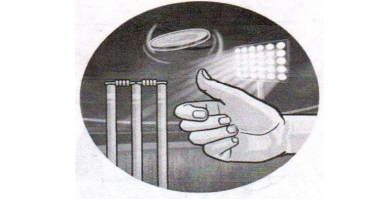
\includegraphics[width=\columnwidth]{./figs/Screenshot (19).png}
        \caption{Tossing a coin}
        \label{fig:2022/probability/fig1.png}
    \end{figure}

Based on the above information, answer the following questions :
\begin{enumerate}[label=(\alph*)]
 \item  If such a coin is tossed $2$ times, then find the probability 
distribution of number of tails.
 
 \item Find the probability of getting at least one head in three tosses of 
such a coin. 
\end{enumerate}

\item Two cards are drawn successively with replacement from a well shuffled pack of $52$ cards. Find the probability distribution of the number of spade cards.

\item A pair of dice is thrown and the sum of the numbers appearing on the dice is observed to be $7$. Find the probability that the number $5$ has appeared on atleast one die.

\item In \figref{fig:2022/probability/fig2.png}, A shopkeeper sells three types of flower seeds $A1$, $A2$, $A3$. They are sold in the form of a mixture, where the proportions of these seeds are $4:4:2$, respectively. The germination rates of the three types of seeds are $45\%$, $60\%$ and $35\%$ respectively.

\begin{figure}[H]
        \centering
        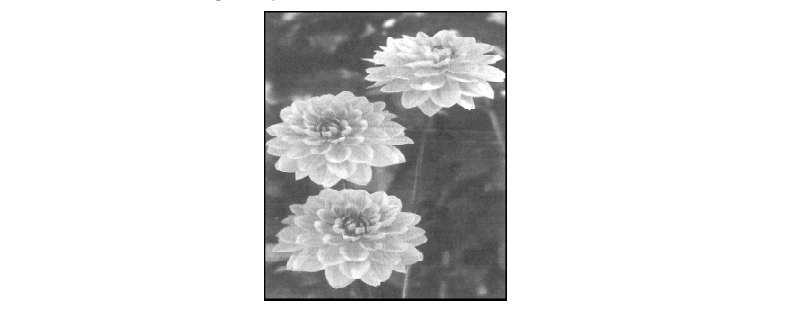
\includegraphics[width=\columnwidth]{./figs/Screenshot (23).png}
        \caption{Three Types of Flower Seeds}
        \label{fig:2022/probability/fig2.png}
    \end{figure}

    Based on the above information:
    
    \begin{enumerate}[label=(\alph*)]
    
 \item Calculate the probability that a randomly chosen seed will germinate;
 
 \item Calculate the probability that the seed is of type $A2$, given that a randomly chosen seed germinates.

\end{enumerate}

\item Three friends $A$, $B$ and $C$ got their photograph clicked. Find the 
probability that $B$ is standing at the central position, given that $A$ is 
standing at the left corner. 

\item In \figref{fig:2022/probability/fig3.png} A coin is tossed twice. The following table shows the probability 
distribution of number of tails :
\begin{figure}[H]
        \centering
        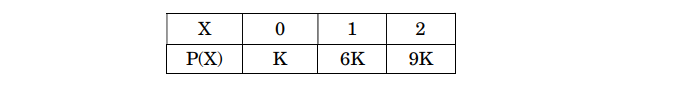
\includegraphics[width=\columnwidth]{./figs/Screenshot (28).png}
        \caption{Probability Distribution of number of tails}
        \label{fig:2022/probability/fig3.png}
    \end{figure}

    \begin{enumerate}[label=(\alph*)]
    
 \item  Find the value of $K$. 
 
 \item  Is the coin tossed biased or unbiased ? Justify your answer.

\end{enumerate}

\item In \figref{fig:2022/probability/fig4.png} In a game of Archery, each ring of the Archery target is valued. The 
centre most ring is worth $10$ points and rest of the rings are allotted 
points $9$ to $1$ in sequential order moving outwards.

Archer A is likely to earn $10$ points with a probability of $0·8$ and Archer $B$ 
is likely the earn $10$ points with a probability of $0·9$.

\begin{figure}[H]
        \centering
        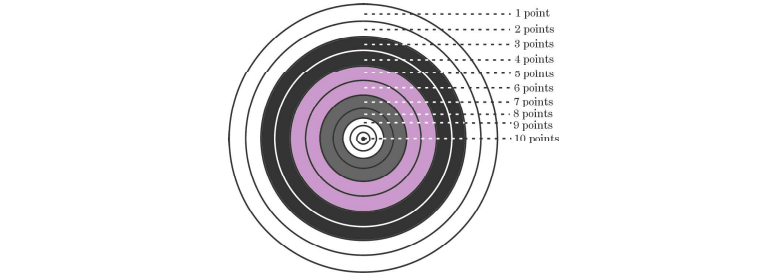
\includegraphics[width=\columnwidth]{./figs/Screenshot (26).png}
        \caption{Ring of the Archery Target}
        \label{fig:2022/probability/fig4.png}
    \end{figure}

Based on the above information, answer the following questions : 
If both of them hit the Archery target, then find the probability that 

\begin{enumerate}[label=(\alph*)]
    
 \item  exactly one of them earns $10$ points.
 
 \item  both of them earn $10$ points.

\end{enumerate}


\item 
\begin{enumerate}[label=(\alph*)]
    
 \item  Events $A$ and $B$ are such that
 P(A) =  $\frac{1}{2}$ , P(B) =  $\frac{7}{12}$  and $ P( \overline{A}  \cup  \overline{B} )= \frac{1}{4}$ Find whether the events $A$ and $B$ are independent or not.
 
 \item  A box $B_{1}$ contains $1$ white ball and $3$ red balls.Another box $B_{2}$ contains $2$ white balls and $3$ red balls.If one ball is drawn at random from each of the boxes $B_{1}$ and $B_{2}$ then find the probability that the two balls drawn are of the same colour.
 
\end{enumerate}

 \item There are two boxes, namely box-I and box-II. Box-I contains $3$ red and $6$ black balls. Box-II contains $5$ red and $5$ black balls. One of the two boxes, is selected at random and a ball is drawn at random. The ball drawn is found to be red. Find the probability that this red ball comes out from box-II.

\item In a toss of three different coins, find the probability of coming up of three heads, if it is known that at least one head comes up.

\item Two rotten apples are mixed with $8$ fresh apples. Find the probability distribution of number of rotten apples, if two apples are drawn at random, one-by-one without replacement.

\item A laboratory blood test is $98\%$ effective in detecting a certain 
disease when it is in fact, present. However, the test also yields 
a false positive result for $0·4\%$ of the healthy person tested. 
From a large population, it is given that 0·2$\%$ of the population 
actually has the disease. 
Based on the above, answer the following questions : 

  \begin{enumerate}[label=(\alph*)]
    
 \item One person, from the population, is taken at random and 
given the test. Find the probability of his getting a 
positive test result.  
 
 \item  What is the probability that the person actually has the 
disease, given that his test result is positive ?

\end{enumerate}

\item Two cards are drawn from a well-shuffled pack of playing 
cards one-by-one with replacement. The probability that the 
first card is a king and the second card is a queen is 

\begin{enumerate}[label=(\alph*)]
    
 \item $\frac{1}{13} + \frac{1}{13}$
 
 \item $\frac{1}{13} \times \frac{4}{51}$

 \item $\frac{4}{52} \times \frac{3}{51}$
 
 \item $\frac{1}{13} \times \frac{1}{13}$ 

\end{enumerate}

\item In \figref{fig:2022/probability/fig5.png} If $X$ is a random variable with probability distribution as given 
below :
\begin{figure}[H]
        \centering
        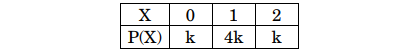
\includegraphics[width=\columnwidth]{./figs/Screenshot (32).png}
        \caption{Probability Distribution}
        \label{fig:2022/probability/fig5.png}
    \end{figure}

The value of $k$ and the mean of the distribution respectively 
are

 \begin{enumerate}[label=(\alph*)]
    
 \item  $\frac{1}{7}$,1 
 
 \item  $\frac{1}{6}$,2

 \item  $\frac{1}{6}$,1

 \item  $\frac{1}{6}$

\end{enumerate}


\item For two events $A$ and $B$ if P(A) = $\frac{4}{10}$, P(B) = $\frac{8}{10}$ and 
$ P(B \mid A)$=$\frac{6}{10}$, then find $ P(A \cup B)$.

\item Bag I contains $4$ red and $3$ black balls. Bag II contains $3$ red 
and $5$ black balls. One of the two bags is selected at random 
and a ball is drawn from the bag, which is found to be red. 
Find the probability that the ball is drawn from Bag II.

\item Two cards are drawn successively without replacement from a 
well-shuffled pack of $52$ cards. Find the probability 
distribution of the number of aces and hence find its mean.
\newpage

\item The probability of solving a specific question independently by $A$ and $B$ 
are $\frac{1}{3}$ and $\frac{1}{5}$ respectively. If both try to solve the question independently, 
the probability that the question is solved is 

\begin{enumerate}[label=(\alph*)]
    
 \item  $\frac{7}{15}$
 
 \item  $\frac{8}{15}$
 
 \item  $\frac{2}{15}$
 
 \item  $\frac{14}{15}$

\end{enumerate}

\item A card is picked at random from a pack of $52$ playing cards. Given that 
the picked up card is a queen, the probability of it being a queen of 
spades is ?

\item A bag contains $19$ tickets, numbered $1$ to $19$. A ticket is drawn at random 
and then another ticket is drawn without replacing the first one in the 
bag. Find the probability distribution of the number of even numbers on 
the ticket.

\item Find the probability distribution of the number of successes in two tosses 
of a die, when a success is defined as ‘‘number greater than $5$’’.

\item The random variable $X$ has a probability function $P(x)$ as defined below, 
where $k$ is some number :

\begin{align}
    p(x) = \begin{cases}
        k, & \text{if } x = 0, \\
        2k, & \text{if } x = 1, \\
        3k, & \text{if } x = 2, \\
        0, & \text{otherwise.}
    \end{cases}
\end{align}

Find :
\begin{enumerate}[label=(\roman*)]
 \item The value of $k$
 
 \item $P(X < 2)$, $P(X \leq 2)$, $P(X\ \geq 2)$
 
 \end{enumerate}

\item Consider the following hypothesis :

\begin {align}
H0 : \mu =  35\\
H1 : \mu \neq 35
\end{align}
A sample of $81$ items is taken whose mean is $37·5$ and the standard deviation is $5$. Test the hypothesis at $5\%$ level of significance.

[Given : Critical value of $Z$ for a two-tailed test at $5\%$ level of significance is $1.96$]

\item In \figref{fig:2022/probability/fig6.png} Fit a straight line trend by the method of least squares and find the trend 
value for the year $2008$ for the following data :

\begin{figure}[H]
        \centering
        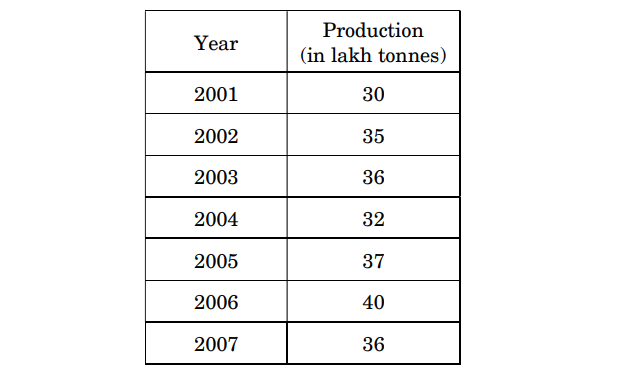
\includegraphics[width=\columnwidth]{./figs/Screenshot (37).png}
        \caption{Years and Production}
        \label{fig:2022/probability/fig6.png}
    \end{figure}
\end{enumerate}

\section{2020}
\subsection{10}
\begin{enumerate}
\item If the probability of an event $E$ happening is $0.023$,then $P(\overline{E})=\underline{\hspace{2cm}}$.
\item Read the following passage and answer the questions given at the end:\newline\textbf{Diwali Fair}\newline A game in booth Diwali Fair involves using a spinner first.Then,if the spinner stops on an even member,the player is allowed to pick a marble from a bag.The spinner and the marbles in the bag are represented in \figref{fig:PROB.PNG}.\newline Prizes are given,when a block marble is picked.Shooter plays the game once.
\begin{figure}[H]
\centering
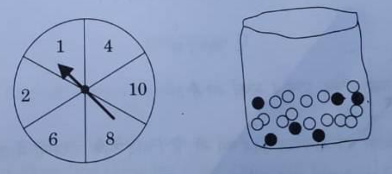
\includegraphics[width=\columnwidth]{figs/PROB.PNG}
\caption{A bag contains of marbles}
\label{fig:PROB.PNG}
\end{figure}
\begin{enumerate}[label=(\roman*)]
\item what is the probability that she will be allowed to pick a mobile from the bag$?$
\item suppose she is allowed to pick a marble from the bag,what if the probability of getting a prize,when it is given that the bag contains $20$ balls out of which $6$ came black$?$
\end{enumerate}
\end{enumerate}

\subsection{12}
\begin{enumerate}
\item A fair dice is thrown two times.Find the probability distribution of the number of sixes. Also determine the mean of the number of sixes.
\item A card from a pack of $52$ cards is lost.From the remaining cards of the pack ,two cards are drawn randomly one-by-one without replacement and are found to be both kings.Find the probability of the last card being a king.
\end{enumerate}

\section{2019}
\subsection{12}
\begin{enumerate}
\item If $P(not A) =0.7$, $P(B)=0.7$ and $P(B\mid A)=0.5$, then find $P(A\mid B)$.

\item A coin is tossed $5$ times. What is the probability of getting 
\begin{enumerate}[label=(\roman*)]
    \item $3$ heads
    \item at most $3$ heads
\end{enumerate}

\item Find the probability distribution of $X$, the number of heads in a simultaneous toss of two coins.

\item There are three coins. One is a two-headed coin, another is a biased coin that comes up heads $75\%$ of the time and the third is an unbiased coin. One of the three coins is chosen at random and tossed. If it shows heads, what is the probability that it is the two-headed coin ?

\item A bag contains $5$ red and $4$ black balls, a second bag contains $3$ red and $6$ black balls. One of the two bags is selected at random and two balls are drawn at random (without replacement) both of which are found to be red. Find the probability that the balls are drawn from the second bag.

\item In a multiple choice examination with three possible answers for each of the five questions, what is the probability that a candidate would get four or more correct answers just by guessing ?

\item The probabilities of solving a specific problem independently by $A$ and $B$ are $\frac{1}{3}$ and $\frac{1}{5}$ respectively. If both try to solve the problem independently, find the probability that the problem is solved.

\item There are three coins. One is a coin having tails on both faces, another is a biased coin that comes up tails $70\%$ of the time and the third is an unbiased coin. One of the coins is chosen at random and tossed, it shows tail. Find the probability that it was a coin with tail on both the faces.
\end{enumerate}


\item Let $X$ be a random variable which assumes values $x_1, x_2, x_3, x_4$ such that 
\begin{align*}
2P\brak{X = x_1} = 3P\brak{X = x_2} = P\brak{X = x_3} = 5P\brak{X = x_4}.
\end{align*}
Find the probability distribution of $X$.

\item Mother, father and son line up at random for a family photo. If $A$ and $B$ are two events given by $A$ = Son on one end, $B$ = Father in the middle, find $P(B\mid A)$.

\item A coin is tossed $5$ times. Find the probability of getting \begin{enumerate}[label=\roman*.]
    \item  at least $4$ heads
    \item at most $4$ heads.
    \end{enumerate}
    
    \item There are two boxes I and II. Box I contains $3$ red and $6$ black balls. Box II contains $5$ red and $'n'$ black balls. One of the two boxes, box I and box I is selected at random and a ball is drawn at random. The ball drawn is found to be red. If the probability that this red ball comes out from box I is $\dfrac{3}{5}$,find the value of $'n'$.

\item Find the mean and variance of the random variable $X$ which denotes the number of doublets in four throws of a pair of dice.


\item A bag contains $5$ red and $3$ black balls and another bag contain $2$ red and $6$ black balls. Two balls are drawn at random (without replacement) from one of the bags an both are found to be red. Find the probability that balls are drawn from the first bag.                 
\item A card from a pack of $52$  playing cards is lost. From the remaining cards of the pack, two cards are drawn at random (without replacement) and both are found to be spades. Find the probability of the lost card being a spade. 
\item In answering a question on a multiple choice questions with four choices in each question out of which only one is correct a student either guesses or copies or knows the answer. The probability that he makes a guess is $\dfrac{1}{4}$ and the probability that he copies is also $\dfrac{1}{4}$. The probability that the answer is correct given that he copied it is $\dfrac{3}{4}$. Find the probability that he knows the answer to the question given that he correctly answered it.


  \item $12$ cards numbered $1$ to $12$ (one number on one card), are placed in a box and mixed up thoroughly. Then a card is drawn at random from the box. If it is known that the number on the drawn card is greater than $5$, find the probability that the card bears an odd number.

    \item Out of $8$ outstanding students of a school, in which there are $3$ boys and $5$ girls, a team of $4$ students is to be selected for a quiz competition. Find the probability that $2$ boys and $2$ girls are selected.

    \item In a multiple choice examination with three possible answers for each of the five questions, what is the probability that a candidate would get four or more correct answers just by guessing ?

    \item An insurance company insured $3000$ cyclists,  $6000$ scooter drivers and $9000$ car drivers. The probability of an accident involving a cyclist, a scooter driver and a car driver are $0.3$, $0.05$ and $0.02$ respectively. One of the insured persons meets with an accident. What is the probability that he is a cyclist ?
   \end{enumerate}


\item If $P\brak{A}=0.6, P\brak{B}=0.5$ and $P\brak{\dfrac{B}{A}}=0.4$ find $P\brak{A \cup B}$ and $P\brak{\dfrac{A}{B}}$.

\item Four cards are drawn one by one with replacement from a well-shuffled deck of playing cards. Find the probability that at least three cards are diamonds.

\item The Probability of two students $A$ and $B$ coming to school on time are $\dfrac{2}{7}$ and $\dfrac{4}{7}$ respectively, Assuming that the events '$A$ coming on time' and '$B$ coming on time' are independent find the probability of only one of them coming to school on time.

\item If $A$ and $B$ are independent events with $P(A)=\dfrac{3}{7}$ and $P(B)=\dfrac{2}{5}$, then find $P(A' \cap B')$
\end{enumerate}

\section{2019}
\subsection{10}
\begin{enumerate}
\item A bag contains $15$ balls, out of which some are white and the others are black. If the probability of drawing a black ball at random from the bag is $\frac{2}{3}$, then find how many white balls are there in the bag.

\item A card is drawn at random from a pack of $52$ playing cards. Find the probability of drawing a card which is neither a spade nor a king.

\item A die is thrown once. Find the probability of getting
\begin{enumerate}
    \item a prime number
    \item an odd number. 
\end{enumerate}

\item Three different coins are tossed simultaneously. Find the probability of getting exactly one head.

\item A die is thrown twice. Find the probability that
\begin{enumerate}
\begin{item}
  $5$ will come up at least once .
 \item $5$ will not come up either time .
\end{item}
\end{enumerate}

\item The probability of selecting a blue marble at random from a jar that contains only blue, black and green marbles is $\frac{1}{5}$. The probability of selecting a black marble at random from the same jar is $\frac{1}{4}$. If the jar contains $11$ green marbles, find the total number of marbles in the jar.

\end{enumerate}

\section{2018}
\subsection{10}
\begin{enumerate}
	\item Two different dice are tossed together. Find the probability:

		\begin{enumerate}[label=(\roman*)]
	\item of getting a doublet
	\item of getting a sum $10$, of the numbers on the two dice.
\end{enumerate}
\item An integer is choosen at random between $1$ and $100$. Find the probability that it is: 

	\begin{enumerate}[label=(\roman*)]
		\item divisible by $8$.
		\item not divisible by $8$.
	\end{enumerate}


\section{12}
\begin{enumerate}

\item A coin is tossed $5$ times. What is the probability of getting (i) $3$ heads,
 (ii) at most $3$ heads ?
\item Find the probability distribution of $X$, the number of heads in a simultaneous toss of two coins.
\item If $P\brak{not A} =0.7, P\brak{B}=0.7$ and $P\brak{B\mid A}=0.5$, then find $P\brak{A\mid B}$.
\item A bag contains $5$ red and $4$ black balls, a second bag contains $3$ red and $6$ black balls. One of the two bags is selected at random and two balls are drawn at random \brak{without replacement} both of which are found to be red. Find the probability that the balls are drawn from the second bag.      
\end{enumerate}






\chapter{Construction}
%\subsection{9}
%\documentclass{article}
%\usepackage{amsmath}
%\usepackage{amssymb}
%\usepackage{amsfonts}
%\usepackage{titling}
%\usepackage{graphicx}

%\providecommand{\abs}[1]{\left\vert#1\right\vert}
%\let\vec\mathbf

%\begin{document}

%\title{\textbf{CONSTRUCTION}}
%\date{}
%\maketitle
\begin{enumerate}


  \item In the given figure, $XZ$ is parallel to $BC$. $AZ$ = 3cm, $ZC$ = 2cm, $BM$ = 3cm and $MC$ = 5cm. Find the length of $XY$.
    \begin{figure}[h!]
      \centering
      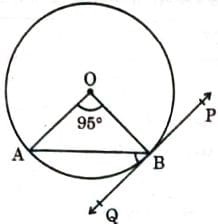
\includegraphics [width=\columnwidth] {figs/fig1.jpg}
      \caption{Isosceles Triangle}
      \label{fig:fig1.jpg}
    \end{figure}

  \item In the given figure, $DE$ $||$ $BC$. If $AD$ = 2units, $DB$ = $AE$ = 3units and $EC$ = $x$units, then find the value of $x$ is:\\

    \begin{figure}[h!]
      \centering
      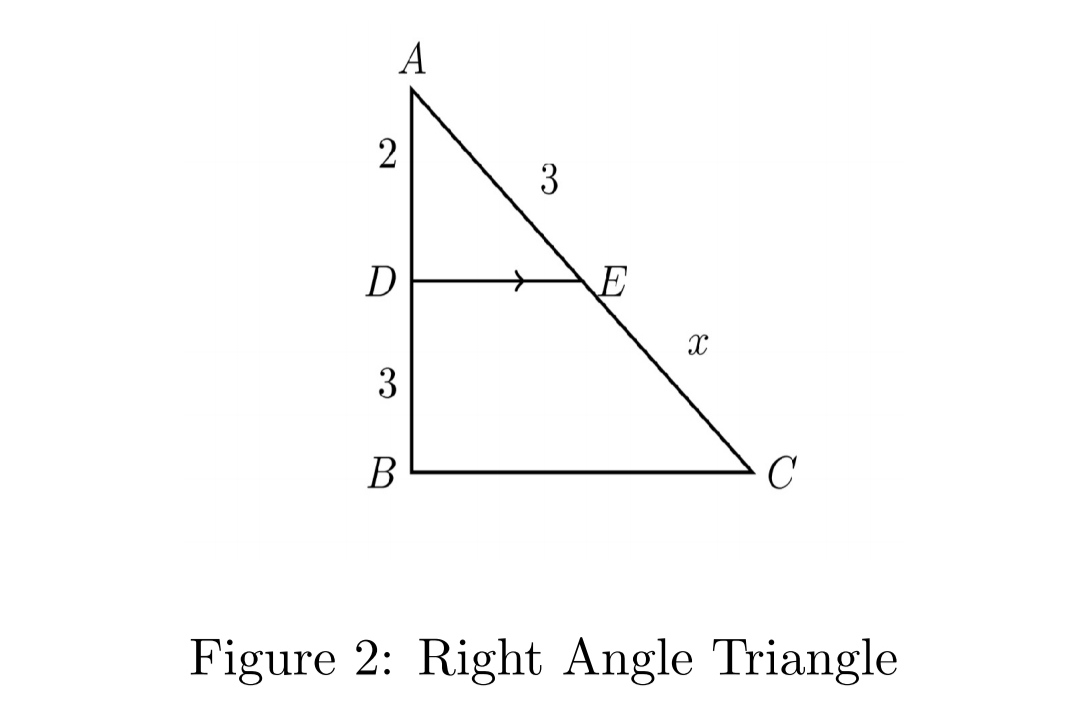
\includegraphics [width=\columnwidth] {figs/fig2.jpg}
      \caption{Right Angle Triangle}
      \label{fig:fig2.jpg}
    \end{figure}

      \begin{enumerate}
        \item 2
        \item 3
        \item 5
        \item $\frac{9}{2}$
      \end{enumerate}

    \newpage

  \item In the given figure, $\Delta ABC$ and $\Delta DBC$ are on te same base $BC$. If $AD$ intersects $BC$ at $\vec{O}$, prove that $\frac { ar(\Delta ABC)}{ar (\Delta DBC)}$ = $\frac{AO}{DO}$.

    \begin{figure}[h!]
      \centering
      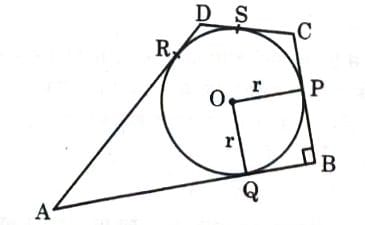
\includegraphics [width=\columnwidth] {figs/fig3.jpg}
      \caption{Triangles with same base}
      \label{fig:fig3.jpg}
    \end{figure}

\end{enumerate}
%\end{document}

\section{2022}
\subsection{10}
\begin{enumerate}[label=\thesection.\arabic*.,ref=\thesection.\theenumi]
\numberwithin{equation}{enumi}
\numberwithin{figure}{enumi}
\numberwithin{table}{enumi}
\item In figure,\figref{fig:rightangled4} BN and CM are medians of a $\triangle$ ABC right-angled at A. Prove that \begin{align}4(BN^2 +CM^2) = 5BC^2\end{align} 
\begin{figure}[!ht]
\centering
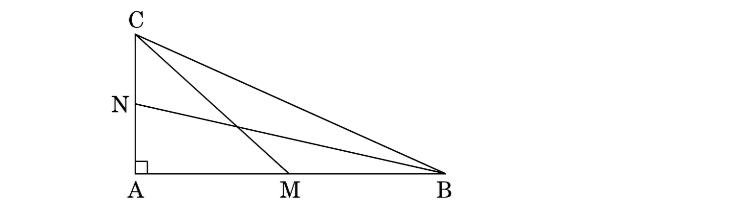
\includegraphics[width=\columnwidth]{figs/rightangled}
\caption{Right-angled triangle}
\label{fig:rightangled4}
\end{figure}
\item $\vec{Case Study - 1:}$
\begin{center}
$\vec{Kite Festival}$\\
\end{center}
Kite festival is celebrated in many countries at different times of the year. in India, every year 14th
January is celebrated as international kite Day. on his day many people visit India and participate in the festival by flying various kinds of kites.
\\The picture given below\figref{fig:kites5} , three kites flying together.
\begin{figure}[!ht]
\centering
\includegraphics[width=\columnwidth]{figs/kites}
\caption{kites flying to gether}
\label{fig:kites5}
\end{figure}
\\In \figref{fig:kites5}, the angles of elevation of two kites (point C) are found to be $\degree{30}$ and  $\degree{60}$ respectively. Taking \begin{align}AD = 50 m\end{align} and\begin{align} BE = 60 m\end{align}
find 
\begin{enumerate}
\item The length of string used (take them straight) for kites A and B as shown in the figure.
\item The distance 'd' between these two kites
\end{enumerate}
\end{enumerate}
	

\section{2021}
\subsection{10}
%\documentclass{article}
%\usepackage{amsmath} 
%\let\vec\mathbf
%\usepackage{gensymb}
%\usepackage{textcomp}
%\usepackage{enumitem}
%\begin{document}
%\section*{\centering Construction}
\begin{enumerate}[label=\thesection.\arabic*.,ref=\thesection.\theenumi]
\numberwithin{equation}{enumi}
\numberwithin{figure}{enumi}
\numberwithin{table}{enumi}
\item Check whether $13$ cm, $12$ cm, $5$ cm can be the sides of a right triangle.
\item \begin{enumerate}
    \item If a $PL$ and $PM$ are two tangents to a circle with center $\vec{O}$ from an external point $\vec{P}$ and $PL=4$ cm, find the length of $OP$, where radius of the circle is $3$ cm.
    \item Find the distance between two parallel tangents of a circle of radius $2.5$ cm.
\end{enumerate}
    \item 
    \begin{enumerate}
    \item $\vec{D}$ and $\vec{E}$ are points on the sides $CA$ and $CB$ respectively of  a triangle $ABC$, right-angled at $\vec{C}$.
    
    Prove that $AE^2+BD^2=AB^2+DE^2$.
    
    \item Diagonals of a trapezium $ABCD$ with $AB\parallel DC$ intersect each other at the point $\vec{O}$. If $AB=2CD$, find the ratio of the areas of triangles $AOB$ and $COD$.
    \end{enumerate}

    \item Answer any \textbf{four} of the following questions :
      \begin{enumerate}[label=(\roman*)]
        \item Given $\triangle ABC \sim \triangle PQR$. If $\frac{AB}{PQ}=\frac{1}{3}$,then $\frac{ar(\triangle ABC)}{ar(\triangle PQR)}$ is 
        \begin{enumerate}[label=(\Alph*)]
            \item $\frac{1}{3}$
            \item $3$
            \item $\frac{2}{3}$
            \item $\frac{1}{9}$
        \end{enumerate}
        
        \item The length of an altitude of an equilateral triangle of side $8$ cm is
        
          \begin{enumerate}[label=(\Alph*)]
            \item $4$ cm
            \item $4\sqrt{3}$ cm
            \item $\frac{8}{3}$ cm
            \item $12$ cm
        \end{enumerate}
        
        \item In $\triangle PQR$, $PQ=6\sqrt{3}$ cm, $PR=12 cm$ and $QR = 6$ cm. The measure of angle $\vec{Q}$ is
        
        \begin{enumerate}[label=(\Alph*)]
            \item $120\degree$
            \item $60\degree$
            \item $90\degree$
            \item $40\degree$
        \end{enumerate}
        
        \item If $\triangle ABC\sim\triangle PQR$ and $\angle B=46\degree$ and $\angle R=69\degree$, then the measure of $\angle$A is
        \begin{enumerate}[label=(\Alph*)]
            \item $65\degree$
            \item $111\degree$
            \item $44\degree$
            \item $115\degree$
        \end{enumerate}
        
        \item $\vec{P}$ and $\vec{Q}$ are the points on the sides $AB$ and $AC$ respectively of a $\triangle ABC$ such that $PQ\parallel BC$. If $AP:PB=2:3$ and $AQ=4$ cm,then $AC$ is equal to

        \begin{enumerate}[label=(\Alph*)]
            \item $6$ cm
            \item $8$ cm
            \item $10$ cm
            \item $12$ cm
        \end{enumerate}
        \end{enumerate}
        \item Write the steps of construction of drawing a line segment $AB=4.8$ cm and finding a point $\vec{P}$ on it such that $AP=\frac{1}{4}AB$.
        
        \item Answer any \textbf{four} of the following questions :
        \begin{enumerate}[label=(\roman*)]
        \item $ABC$ and $BDE$ are two equilateral triangles such that $\vec{D}$ is the mid-point of $BC$. The ratio of the areas of the triangles $ABC$ and $BDE$ is
        \begin{enumerate}[label=(\Alph*)]
            \item 2:1
            \item 1:2
            \item 4:1
            \item 1:4
        \end{enumerate}
        
        \item In $\triangle$ ABC , $AB=4\sqrt{3}$ cm, $AC=8$ cm and $BC=4$ cm. The angle $B$ is

        \begin{enumerate}[label=(\Alph*)]
            \item $120\degree$
            \item $90\degree$
            \item $60\degree$
            \item $45\degree$
        \end{enumerate}
         
        \item The perimeters of two similar triangles are $35$ cm and $21$ cm respectively.  If one side of the first triangle is $9$ cm, then the corresponding side of the second triangle is 
        
         \begin{enumerate}[label=(\Alph*)]
            \item $5.4$ cm
            \item $4.5$ cm
            \item $5.6$ cm
            \item $15$ cm
        \end{enumerate}
        
        \item In a $\triangle ABC$ , $\vec{D}$ and $\vec{E}$ are points on the sides $AB$ and $AC$ respectively such that $DE\parallel BC$ and $AD:DB=3:1$. If $AE=3.3 $ cm, then $AC$ is equal to
        \begin{enumerate}[label=(\Alph*)]
            \item $4$ cm
            \item $1.1$ cm
            \item $4.5$ cm
            \item $5.5$ cm
        \end{enumerate}
        
        \item In an isosceles triangle $ABC$, if $AC=BC$ and $AB^2=2AC^2$, the $\angle$C is equal to
        \begin{enumerate}[label=(\Alph*)]
            \item $30\degree$
            \item $45\degree$
            \item $60\degree$
            \item $90\degree$
        \end{enumerate}
        \end{enumerate}
\end{enumerate}
%\end{document}


\section{2020}
\subsection{10}
\begin{enumerate}
	\item Draw a circle of radius $3.5 cm$. Take a point $P$ outside the circle at a distance of $7 cm$ from the centre of the circle and construct a pair of tangents to the circle from that point.
	\item Contruct a $\triangle ABC $ with sides $BC = 6 cm$, $AB = 5 cm$ and $\angle ABC = 60\degree$. Then construct a triangle whose sides are $\frac{3}{4}$ of the corresponding sides of $\triangle ABC$.
	\item In \figref{fig:Construction-1.jpg}, $DE \parallel BC $. If $\frac{AD}{DB}=\frac{3}{2}$ and $AE = 2.7 cm$, then $EC$ is equal to
		\begin{enumerate}
		\item $2.0 cm$ 
                \item $1.8 cm$
		\item $4.0 cm$
		\item $2.7 cm$
		\end{enumerate}
		\begin{figure}[!ht]
			\begin{center}
				\includegraphics[width=\columnwidth]{figs/Construction-1.jpg}
			\end{center}
			\caption{}
			\label{fig:Construction-1.jpg}
		\end{figure}
		\newpage
	\item In \figref{fig:Construction-2.jpg}, if $PQ \parallel BC$ and $PR \parallel CD$ that $\frac{QB}{AQ} = \frac{DR}{AR}$.



		\begin{figure}[!ht]
			\begin{center}
				\includegraphics[width=\columnwidth]{figs/Construction-2.jpg}
			\end{center}
			\caption{}
			\label{fig:Construction-2.jpg}
		\end{figure}
\end{enumerate}


\section{2019} 
\subsection{10}
\begin{enumerate}
\item In $\triangle ABC$ \figref{fig:Fig_2}, $AD \perp BC$. Prove that\\
$AC^2 = AB^2 + BC^2 - 2BC \times BD $
\begin{figure}[H]
    \centering
    \includegraphics[width=\columnwidth]{figs/cons2.png}
    \caption{}
    \label{fig:Fig_2}
\end{figure}

\item Draw a circle of radius $4$ cm. From a point $6$ cm away from its centre, construct a pair of tangents to the circle and measure their lengths.

\item Construct a triangle with sides $5cm$, $6cm$ and $7cm$ and then another triangle whose sides are $\frac{3}{5}$ of the corresponding sides of the first triangle.

\item Let $\triangle ABC  \thicksim  \triangle DEF$  and their areas be respectively, $64cm^2$ and $121cm^2$. If $EF=15.4cm$, find $BC$.

\item Prove that the sum of the squares of the sides of a rhombus is equal to the sum of the squares of its diagonals. 

\item In \figref{fig:Fig_3}, $BL$ and $CM$ are medians of a $\triangle ABC$ right-angled at $A$. Prove that $4(BL^2 + CM^2)= 5 BC^2$. 
\begin{figure}[H]
    \centering
    \includegraphics[width=\columnwidth]{figs/cons1.png}
    \caption{Triangle ABC}
    \label{fig:Fig_3}
\end{figure}

\item In  \figref{fig:Figh_1}, $ABC$ is an isosceles triangle right angled at $C$ with $AC = 4 cm$. Find the length of $AB$.
\begin{figure}[H]
    \centering
    \includegraphics[width=\columnwidth]{figs/img1.jpg}
    \caption{Triangle $ABC$}
    \label{fig:Figh_1}
\end{figure}

\item In  \figref{fig:Figh_2}, $DE \parallel BC$. Find the length of side $AD$, given that $AE = 1.8 cm$, $ BD = 7.2 cm$ and $ CE = 5.4 cm$.
\begin{figure}[H]
    \centering
    \includegraphics[width=\columnwidth]{figs/img2.jpg}
    \caption{Triangle $ABC$ }
    \label{fig:Figh_2}
\end{figure}

\item Two right triangles $ABC$ and $DBC$ are drawn on the same hypotenuse $BC$ and on the same side of $BC$. If $AC$ and $BD$ intersect at $P$, prove that $AP \times PC = BP \times DP$.

\item Construct an equilateral $\triangle ABC$ with each side $5 cm$. Then construct another triangle whose sides are $\frac{2}{3}$ times the corresponding sides of $\triangle ABC$.

\item Diagonals of a trapezium $PQRS$ intersect each other at the point $O$,
$PQ \parallel RS$ and $PQ = 3RS$. Find the ratio of the areas of triangles $POQ$ and $ROS$.
\end{enumerate}

\section{2018} 
\subsection{10}
\begin{enumerate}
	\item In an equilateral $\triangle$ ABC, D is a point on side BC such that $ BD =\frac{1}{3}BC$. Prove that $9(AD)^2 = 7(AB)^2$.
	\item Prove that, in a right triangle, the  square on the hypotenuse is equal to sum of the squares on the other two sides.
	\item Prove that the area of an equilateral triangle described on one side of the square is equal to half of the area of the equilateral triangle described on one of its diagonal.
	\item If the area of two similar triangles are equal, prove that they are congruent.
	\item Draw a triangle ABC with $BC=6 cm, AB=5 cm$ and $\angle{ABC}=60\degree$. Then construct a triangle whose sides are $\frac{3}{4}$ of the corresponding sides of the $\triangle ABC$.

	\item Given $\triangle ABC \sim  \triangle PQR$, if $\frac{AB}{PQ} = \frac{1}{3}$, then find $\frac{ar \triangle ABC}{ar \triangle PQR}$.
\end{enumerate}







\chapter{Optimization}
\section{2023}

\begin{enumerate}
	\item The objective function $Z = ax+by$ of an LLP has maximum value 42 at (4,6) and minimum value 19 at (3,2).Which of the following is true?
		
  		\begin{enumerate}
				\item $a=9,b=1$
		        	\item $a=5,b=2$
				\item $a= 3,b=5$
				\item $a=5,b=3$
			
		\end{enumerate}
		
	\item The corner point of the feasible region of a linear programming problem are (0,4), (8,0)and ($\frac{20}{3}$,$\frac{4}{3}$).if $ Z=30x+24y $ is the objective fnction, then ( maximum value of Z-minimum value of Z) is equal to 
		
		\begin{enumerate}
				\item 40
				\item 96
				\item 120
				\item 136
		\end{enumerate}
		
		
	\item 
	 Solve the following linear programming problem graphically :
\begin{align}
	Maximum:& Z=x+2y \nonumber \\
	subject to constraints 
	     :& x+2y\ge100 ,\nonumber\\
             &  2x-y\le0 ,\nonumber\\
	     &  2x+y\le200 ,\nonumber\\
   	     &   x\ge0 ,y\ge0 .\nonumber
\end{align}
				

			      \item
		Engine displacement is the measure of the cylinder volume swept by all the pistons engine.The piston move inside the cylinder bore \\
		
		\begin{figure}[htbp]
	\includegraphics[width=1 \columnwidth]{./figs/engine.jpg}\\
			\caption{Engine}
			\label{fig:pic}  \end{figure}
		The cylinder bore in the form of circular cylinder open at the top is to be made from a metal sheet of area $ 75 \pi cm^2 $ \\
 	
		Based on the above information,answer the following questions:\\
		
			\begin{enumerate}
				\item if the radius of cylinder is r cm and height is h cm,then write the volme V of cylinder in terms of radius r.
					
				\item Find $ \frac{dV}{dr} $.
					
				\item \begin{enumerate}
						\item Find the radius of cylinder when its volume is maximum.
			
		\item For maximum volume,$h>r$.State true or false and justify.
				
			
				\end{enumerate}
			\end{enumerate}
\end{enumerate}

\section{2021}
\subsection{12}
\begin{enumerate}

\item If the corner points $(3,4)$ and $(5,0)$ of the feasible region in an LPP, give the same maximum value for the objective function $z=ax+by$, where a,b $>$ 0, then we have 


\begin{enumerate}
\item $a=2b$
\item $2a=b$
\item $2a=3b$
\item $3b=2a$
\end{enumerate}

\item A dietician wishes to mix two types of foods in such a way that vitamin contents of the mixture contain at least 8 units of vitamin A and 10 units of vitamin C. Food I contains 2 units/kg of vitamin A and 1 unit/kg of vitamin C. Food II contains 1  unit/kg of vitamin A and 2 units/kg of vitamin C. It costs 1 \rupee 50 per kg to purchase Food I and  \rupee 70 per kg to purchase Food II. Formulate this problem as a Linear Programming Problem for minimizing the cost of such a mixture.

\item Show that of all the rectangles inscribed in a given fixed circle, the square has maximum area.



Find the intervals in which the function f given by $f(x) = \sin x + \cos x, 0 \le x \le 2\pi$ is strictly increasing or strictly decreasing.

\item A company produces two types of goods, A and B that require gold and silver. Each unit of type A requires 3 g of silver and 1 g of gold, while that of type B requires 1 g of silver and 2 g of gold. The company can use at the most 9 g of silver and 8 g of gold. If each unit of type A brings a profit of    \rupee  120  and that of type B   \rupee 150  , then find the number of units of each type that the company should produce to maximize profit.

Formulate the above LPP and solve it graphically. Also, find the maximum profit.


\item Find the intervals in which the function f defined as $f(x) = \sin x + \cos x, 0 \le x \le 2\pi$ is strictly increasing or decreasing.



Prove that the radius of the right circular cylinder of greatest curved surface area which can be inscribed in a given cone is half of that of the cone.

\item Maximize $z=3x + 4y$, if possible,

subject to the constraints :
\begin{align}
 x - y &\le - 1 \\
-x + y &\le 0 \\
x, y &\ge 0
\end{align}


\item A dietician wishes to mix two types of foods F1 and F2 in such a way that the vitamin content of the mixture contains at least 8 units of vitamin A and 10 units of vitamin C. Food F1 contains 2 units/kg of vitamin A  and 1 unit/kg of vitamin C, while Food F2 contains 1 unit/kg of vitamin A and 2units/kg of vitamin C. It costs \rupee  5  per kg to purchase Food F1 and  \rupee  7  per kg to purchase Food F2


Based on the above information, answer the following questions:


\begin{enumerate}
\item To find out the minimum cost of such a mixture, formulate the above problem as a LPP.
\item Determine the minimum cost of the mixture.
\end{enumerate}


\item Find the area bounded by the curves $y = \abs{x - 1}$ and $y = 1$, using integration.

\end{enumerate}

\section{2022}
\subsection{12}
\begin{enumerate}
  
\item A company produces two types of goods, $A$ and $B$, that require gold and
silver. Each unit of type $A$ requires $3g$ of silver and $1g$ of gold, while that of type $B$ requires $1g$ of silver and $2g$ of gold. The company can use at
the most $9g$ of silver and $8g$ of gold. If each unit of type $A$ brings a profit
of \rupee~120 and that of type $B$ \rupee~150, then find the number of units of each type that the company should produce to maximise profit. Formulate the above LPP and solve it graphically. Also, find the maximum profit.
\item Find the maximum value of $7x+6y$ subject to the constrains:
\begin{align}
	x+y &\geq   2\\
	2x+3y &\leq 6\\
	x \geq 0 \text{and} y &\geq 0
\end{align}
\item A window is in the form of a rectangular mounted by a semi-circular opening.The total perimeter of the window to admit maximum light through the whole opening.
\item Divide the number $8$ into two positive numbers such that the sum of the cube of one and the square of the other is maximum.
\item Find the maximum and the minimum values of 
\begin{align}
       z=5x+2y 
\end{align}	
		subject to the constrains:
\begin{align}
	-2x-3y &\leq -6\\
	x-2y &\leq 2\\
	6x+4y &\leq 24\\
	-3x+2y &\leq 3\\
	x \geq 0, y &\geq 0
\end{align}
 
 \item A furniture dealer deals in only two items : chairs and tables. He has \rupee~5,000  to invest and a space to store at most $60$ pieces. A table costs him \rupee~250 and a chair \rupee~50. He sells a table at a profit of \rupee~50 and a chair at
a profit of \rupee~ 15. Assuming that he can sell all the items he buys, how should he invest his money in order that he may maximize his profit ?
Formulate the above as a linear programming problem.
\item The least value of the function 
\begin{align}
	f(x)=2\cos(x) + x
\end{align}
		in the closed interval $\sbrak{0, \frac{\pi}{2}}$ is: 
\begin{enumerate}
    \item  $2$
    \item  $\frac{\pi}{6} + \sqrt{3}$
    \item  $\frac{\pi}{2}$
    \item The least value does not exist.
\end{enumerate}
\item A linear programming problem is as follows:
Minimize 
\begin{align}
	Z=30x+50y 
\end{align}
		subject to the constrains,
\begin{align}
	3x+5y &\geq 15\\
	2x+3y &\leq 18\\
	x \geq 0, y &\geq 0
\end{align}
In the feasible region, the minimum value of $Z$ occurs at 
\begin{enumerate}
    \item a unique point 
    \item no point
    \item infinitely many points 
    \item two points only
\end{enumerate}
\item The area of a trapezium is defined by function $f$
and given by 
\begin{align}
	f(x)=(10+x)\sqrt{100-x^2}
\end{align}
			, then the area when it is maximised is:
\begin{enumerate}
    \item $75cm^2$
    \item $7\sqrt{3}cm^2$
    \item $75\sqrt{3}cm^2$
    \item $5cm^2$
\end{enumerate}
\item For an objective function 
\begin{align}
	Z=ax+by
\end{align}		
		,where $a,b>0$;the corner points of the feasible region determined by a set of constrains (linear inequalities) are $(0,20)$, $(10,10)$, $(30,30)$, and $(0,40)$.The condition on $a$ and $b$ such that the maximum $Z$ occurs at the points $(30,30)$ and $(0,40)$ is: 
\begin{enumerate}
    \item $b-3a=0$
    \item $a=3b$
    \item $a+2b=0$
    \item $2a-b=0$
\end{enumerate}
\item In a linear programming problem, the constrains on the decision variables $x$ and $y$ are $x-3y \geq 0, y \geq 0, 0\leq x \leq 3$.The feasible region 
\begin{enumerate}
    \item is not in the first quadrant
    \item is bounded in the first quadrant 
    \item is unbounded in the first quadrant 
    \item does not exist  
\end{enumerate}
\item Based on the given shaded region in figure \ref{fig:19/2021/041} as the feasible region in the graph, at which point(S) is the objective function 
\begin{align}
	Z=3x+9y 
\end{align}
		maximum?
\begin{figure}[h]
    \centering{}
    \includegraphics[width=\columnwidth]{figs/opti-21-fig1.jpg}
	\caption{Optimization graph}
    \label{fig:19/2021/041}
\end{figure}
\begin{enumerate}
    \item point $B$
    \item point $C$
    \item point $D$
    \item every point on the line segment $CD$   
\end{enumerate}
\item In figure \ref{fig:23/2021/041}, the feasible region for a LPP is shaded.The objective function 
\begin{align}
	Z=2x-3y
\end{align}
		,will be minimum at:
\begin{figure}[h]
    \centering{}
     \includegraphics[width=\columnwidth]{figs/opti-21-fig2.jpg}
	\caption{Optimization graph}
     \label{fig:23/2021/041}                       
\end{figure}
\begin{enumerate}
    \item $(4,10)$
    \item $(6,8)$
    \item $(0,8)$
    \item $(6,5)$
\end{enumerate}
    
\end{enumerate}

\section{2020}
\subsection{12}

\begin{enumerate}
	\item The corner points of the feasible region of an LLP are \brak{0,0},\brak{0,8},\brak{2,7},\brak{5,4} and \brak{6,0}. The maximum profit $P=3x+2y$ occure at the point \underline{\hspace{4cm}}.
\end{enumerate}

\section{2019}
\subsection{12}
\begin{enumerate}
\item A company produces two types of goods, $A$ and $B$, that require gold and silver. Each unit of type $A$ requires $3$ g of silver and $1$ g of gold while that of type $B$ requires $1$ g of silver and $2$ g of gold. The company can use at the most $9$ g of silver and $8$ g of gold. If each unit of type $A$ brings a profit of \rupee $40$ and that of type $B$ \rupee $50$, find the number of units of each type that the company should produce to maximize profit. Formulate the above LPP and solve it graphically and also find the maximum profit.

\item Show that the height of the cylinder of maximum volume that can be inscribed in a sphere of radius $R$ is $\frac{2R}{\sqrt{3}}$. Also find the maximum volume.

\item The volume of a cube is increasing at the rate of $8 cm^3/s$. How fast is the surface area increasing when the length of its edge is $12 cm$ ?
\end{enumerate}

\item $A$ company manufactures two types of novelty souvenirs made of plywood. Souvenirs of type $A$ require $5$ minutes each for cutting and $10$ minutes each for assembling. Souvenirs of type $B$ require $8$ minutes each for cutting and $8$ minutes each for assembling. There are $3$ hours and $20$ minutes available for cutting and $4$ hours available for  assembling. The profit is \rupee $50$ each for type $A$ and \rupee $60$  each for type $B$ souvenirs. How many souvenirs of each type should the company manufacture in order to maximize profit ? Formulate the above LPP and solve it graphically and also find the maximum profit .

\item Find the local maxima and local minima, if any, of the following function. Also find the local maximum and the local minimum values, as the case may be :
\begin{align*}
    f\brak{x}=\sin x + \dfrac{1}{2} \cos 2x,0\leq x \leq \dfrac{\pi}{2}.
\end{align*}

\item Show that the height of a cylinder, which is open at the top, having a given surface area and greatest volume, is equal to the radius of its base.


\item The sum of the perimeters of circle and a square is K is some constant. Prove that the sum of their area is least when the side of the square is twice the radius of the radius of the circle.  
\item Prove that the radius of the right circular cylinder of greatest curved surface area which can be inscribed in a given cone is half of that of the cone.
  \item A company manufactures two types of novelty souvenirs made of plywood. souvenirs of type A require $5$ minutes each for cutting and $10$ minutes each for assembling. Souvenirs of type $B$ require $8$ minutes each for cutting and $8$ minutes each for assembling. There are 3 hours $20$ minutes available for cutting and $4$hours for assembling. The profit for type $A$ souvenirs is \rupee$ 100$ each and for type $B$ souvenirs, profit is \rupee $120$ each. How many souvenirs of each type should the company manufacture in order to maximum the profit ? Formulate the problem as a LPP and then solve it graphically. 



\item An isosceles triangle of vertical angle $2\theta$ is inscribed in a circle  of radius $a$. Show that the area of the triangle is maximum when $\theta =\dfrac{\pi}{6}$.
\end{enumerate}      

\section{2018}
\subsection{12}
\input{2018/optimisation.tex}



\chapter{Algebra}
\section{2020}
\subsection{10}
\documentclass[12pt]{article} 
%\usepackage{listings}
%\usepackage{biblatex}
%\usepackage{hyperref}
%\usepackage{tikz}
%\usepackage{refstyle}
%\usepackage{mathabx}
\usepackage{amssymb}
\usepackage{amsmath}
\usepackage{gensymb}
%\usepackage{caption}
%\usepackage{gensymb}
%\usepackage{float}
%\usepackage{marvosym}
%\usepackage{dashrule}
%\usepackage{tfrupee}
%\usepackage{graphicx}
%\usepackage{graphics}
%\usepackage{subfig}
\usepackage{enumitem}
\usepackage{mathabx}
\providecommand{\brak}[1]{\ensuremath{\left(#1\right)}}
\begin{document}
\title{ALGEBRA}
\date{ \today}
\maketitle
\begin{enumerate}

\item The value(s) of $k$ for which the quadratic equation $2x^2 + kx + 2 = 0$ has equal roots, is 
\begin{enumerate}[label =(\Alph*)]
\item $4$ 
\item $\pm 4$
\item $-4$
\item $0$ 
\end{enumerate}

\item on dividing a polynomial $p(x)$ by $x^2 - 4$,quotient and remainder are found to be $x$ and $3$ respectively. The polynomial $p(x)$ is 
\begin{enumerate}[label =(\Alph*)]
\item $3x^2 + x - 12$
\item $x^3 - 4x + 3$
\item $x^2 + 3x - 4$
\item $x^3 - 4x - 3$
\end{enumerate}

\item Simplest form of 
 \begin{align}
     \frac{1 + \tan^{2}{A}}{1 + \cot^{2}{A}}
 \end{align}is .

\item Write the value of
 \begin{align}
	     \sin^{2}{30\degree} + \cos^{2}{60\degree}
	\end{align}.
\item From the quadratic polynomial, the sum and product  of whose zeroes are $(-3)$ and $2$ respectively.

\item Can $\brak{x^{2} - 1}$ be a reminder while dividing $x^{4} - 3x^{2} + 5x - 9$ by 
$\brak{x^{2}+3}$ ? Justify your answer with reasons.

\item If $A$, $B$ and $C$ are interior angles of $ \triangle ABC$, then show that
	\begin{align}
	    \cos \brak{\frac{B + C}{2}}=\sin \brak{\frac{A}{2}}
	\end{align}
      
\item Prove that : 
        \begin{align}
           (\sin^{4}{\theta} - \cos^{4}{\theta} + 1)\csc^{2}{\theta} = 2 
        \end{align}
  
\item
	Sum of the areas of two squares is $544 m^2$. If the difference of their
perimeters is $32 m$, find the sides of the two squares.

\item
	A motor boat whose speed is $18$km/h in still water takes $1$ hour more to 
go $24$km upstream than to return down stream to the same spot. Find the speed of the stream.

\item Obtain the zeroes of the polynomial
$p(x) = 2x^4 - x^3 - 11x^2 + 5x + 5$ if two zeroes are $\sqrt5$ and $-\sqrt5$.

\item What minimum is added to $2x^3 - 3x^2 + 6x + 7$ so that the resulting
polynomial will be divisible by $x^2 - 4x + 8$ ?
\end{enumerate}
\end{document}  
\section{2020}
\subsection{12}
\documentclass[12pt]{article} 
%\usepackage{listings}
%\usepackage{biblatex}
%\usepackage{hyperref}
%\usepackage{tikz}
%\usepackage{refstyle}
%\usepackage{mathabx}
\usepackage{amssymb}
\usepackage{amsmath}
\usepackage{gensymb}
%\usepackage{caption}
%\usepackage{gensymb}
%\usepackage{float}
%\usepackage{marvosym}
%\usepackage{dashrule}
%\usepackage{tfrupee}
%\usepackage{graphicx}
%\usepackage{graphics}
%\usepackage{subfig}
\usepackage{enumitem}
\usepackage{mathabx}
\providecommand{\brak}[1]{\ensuremath{\left(#1\right)}}
\begin{document}
\title{ALGEBRA}
\date{ \today}
\maketitle
\begin{enumerate}
\item
If
\begin{align}
\cos\brak{\sin^{-1}{\frac{2}{\sqrt{5}}} + \cos^{-1}{x}} = 0
\end{align}
then $x$ is equal to
\begin{enumerate}[label=(\Alph*)]
	\item $\frac{1}{\sqrt{5}}$
	\item $-\frac{2}{\sqrt{5}}$
	\item $\frac{2}{\sqrt{5}}$
        \item $1$
\end{enumerate}
\end{enumerate}
\end{document}  
\section{2023}
\subsection{10}
%\documentclass{article}
%\begin{document}
\begin{enumerate}
 \item If one zero of the polynomial \begin{align} p(x)=6x^2+37x-(k-2) \end{align} is reciprocal of the other, then find the value of $k$?
 \item Find the value of $'p'$ for which one root of the quadratic equation \begin{align} px^2-14x+18=0 \end{align}is 6 times the other?
 \item 
 \begin{enumerate}
  \item prove that \begin{align} \frac{\sin A-2 \sin^3A}{2\cos^3A-\cos A}=\tan A\end{align} 
  \item \begin{align} \sec A (1-\sin A)(\sec A+\tan A)=1\end{align} 
  \end{enumerate}
  \item Which of the following  quadratic equations has sum of its roots as 4?
  \begin{enumerate}
      \item $2x^2-4x+8=0$ 
      \item $-x^2+4x+4=0$
      \item $\sqrt{2x^2}-\frac{4}{\sqrt{2}}x+1=0$ 
      \item $4x^2-4x+4=0$
   \end{enumerate}
   \item if one zero of the polynomial \begin{align} 6x^2+37x-(k-2)\end{align}  is reciprocal of the other,then what is the value of $k$?
   \begin{enumerate}
       \item -4
       \item -6
       \item 6
       \item 4
   \end{enumerate}
   \item The zeroes of the polynomial \begin{align}p(x)=x^2+4x+3\end{align}  are given by:
   \begin{enumerate}
       \item 1,3
       \item -1,3
       \item 1,-3
       \item -1,-3
   \end{enumerate}
\item If $\alpha$ and $\beta$ are the zeroes of the quadratic polynomial $p(x)=x^2-ax-b$, then the value of $\alpha^2 + \beta^2$ is:


\begin{enumerate}
\item $a^2-2b$
\item $a^2+2b$
\item $b^2-2a$
\item $b^2+2a$
\end{enumerate}

\item The below is the Assertion and Reason based question. Two statements are given, one labelled as Assertion(A) and the other is labelled as Reason(R). Select the correct answer to these questions from the codes (a),(b),(c) and (d) as given below.
\begin{enumerate}
\item Both Assertion(A) and Reason(R) are true and Reason(R) is the correct explanation of the Assertion(A).
\item Both Assertion(A) and Reason(R) are true, but Reason(R) is not the correct explanation of the Assertion(A).
\item Assertion(A) is true, but Reason(R) is false.
\item Assertion(A) is false, but Reason(R) is true.\\ 
\textbf{Assertion(A):} The polynomial $p(x)=x^2+3x+3$ has two real zeroes.\\
\textbf{Reason(R):} A quadratic polynomial can have at most two real zeroes.

\end{enumerate}

\item
\begin{enumerate}
\item If 
\begin{align}
    4\cot^2 45\degree - \sec^2 60\degree + \sin^2 60\degree + p = \frac{3}{4}, 
\end{align}
then find the value of $p$.
\item If 
\begin{align}
    \cos A+ \cos^2A=1,
\end{align}then find the value of 
\begin{align}
\sin^2A+\sin^4A.
\end{align}
\end{enumerate}


\item Prove that:\\
\begin{align}
\brak{\frac{1}{\cos\theta}-\cos\theta}\brak{\frac{1}{\sin\theta}-\sin\theta} = \frac{1}{\tan\theta+\cot\theta}
\end{align}


\item The value of k for which the pair of equations $kx=y+2$ and $6x=2y+3$ has infinitely many solutions,
\begin{enumerate}
\item is $k=3$
\item does not exist
\item is $k=-3$
\item is $k=4$
\end{enumerate}


\item If $2\tan A=3$, then the value of $\frac{4sin A + 3\cos A}{4\sin A - 3\cos A}$ is
\begin{enumerate}
\item $\frac{7}{\sqrt{13}}$
\item $\frac{1}{\sqrt{13}}$
\item $3$
\item does not exist
\end{enumerate}


\item If $\alpha$, $\beta$ are the zeroes of a polynomial $p(x)=x^2+x-1$, then $\frac{1}{\alpha}+\frac{1}{\beta}$ equals to 
\begin{enumerate}
\item $1$
\item $2$
\item $-1$
\item $\frac{-1}{2}$
\end{enumerate}

    \item $\brak{\sec^2\theta - 1}\brak{\csc^2\theta - 1}$  is equal to:
    \begin{enumerate}
        \item $-1$
        \item  $1$
        \item  $0$
        \item  $2$
        \end{enumerate}
    \item The roots of equation 
    \begin{align}
        x^2 + 3x - 10 = 0
    \end{align}
    are:
    \begin{enumerate}
        \item $\brak{2,-5}$
        \item $\brak{-2,5}$
        \item $\brak{2,5}$
        \item $\brak{-2,-5}$
    \end{enumerate}
    \item If $\alpha$ , $\beta$ are zeroes of the polynomial $x^2-1$,then value of $\brak{\alpha+\beta}$ is:
    \begin{enumerate}
        \item $2$
        \item $1$
        \item $1$
        \item $0$
    \end{enumerate}
    \pagebreak
   \item  If $\alpha$, $\beta$ are the zeroes of the polynomial
   \begin{align}
       p(x)=4x^2 - 3x -7
   \end{align}
   ,then $\brak{\frac{1}{\alpha}+\frac{1}{\beta}}$ is equal to:
   \begin{enumerate}
       \item $\frac{7}{3}$
       \item $\frac{-7}{3}$
       \item $\frac{3}{7}$
       \item $\frac{-3}{7}$
   \end{enumerate}
   \item  Find the sum and product of the roots of the quadratic equation 
   \begin{align}
       2x^2-9x+4=0
   \end{align}
   \item Find the discriminant of the quadratic equation 
   \begin{align}
       4x^2-5=0
   \end{align}
   and hence comment on the nature of roots of the equation.
   \item Evaluate $2\sec^2\theta+3\csc^2\theta-2\sin\theta\cos\theta$ if
   \begin{align}
      \theta=45\degree
   \end{align}
   
   \item If
   \begin{align}
       \sin\theta-\cos\theta=0
   \end{align}
   ,then find the value of $\sin^4\theta+\cos^4\theta$.

\end{enumerate}
%\end{document}

\section{2022}
\subsection{10}
\begin{enumerate}
    \item If $\sin \theta=0$, then the value of $\tan^2\theta+\cot^2\theta$ is
    \begin{enumerate}
        \item $2$
        \item $4$
        \item $1$
        \item $\frac{10}{9}$
    \end{enumerate}
    \item The value(s) of $k$ for which the quadratic equation 
    \begin{align}
        3x^2 - kx + 3 = 0
    \end{align}
    has equal roots, is (are) 
    \begin{enumerate}
        \item $6$
        \item $-6$
        \item $\pm6$
        \item $9$
    \end{enumerate}
    \item $5\tan^2 \theta - 5\sec^2\theta = \underline{\hspace{2cm}}$
    \item If $\alpha$, $\beta$ are zeroes of the polynomial $2x^2 - 5x - 4$, then $\frac{1}{\alpha}+\frac{1}{\beta}$.
    \item In  \figref{fig:as.jpeg}, a tower stands vertically on the ground. From a point on the ground, which is $80m$ away from the foot of the tower, the angle of elevation of the tower is found to be $30\degree$. Find the height of the tower.
    \begin{figure}[H]
        \centering
        \includegraphics[width=70mm]{figs/as.jpeg}
        \caption{as.jpeg}
        \label{fig:as.jpeg}
    \end{figure}
    \item Solve
    \begin{align}
        9x^2 - 6a^2x + a^4 - b^4 = 0
    \end{align}
    using the quadratic formula.
    \item Show that 
    \begin{align}
        \cos(38\degree) \cos(52\degree) - \sin(38\degree)\sin(52\degree) = \cos(90\degree).
    \end{align}
    \item Prove that 
    \begin{align}
        \frac{\sin\theta}{\cot\theta+\csc\theta} = 2+\frac{\sin\theta}{\cot\theta-\csc\theta}.
    \end{align}
    \item Given 
    \begin{align}
        15 \cot (A) = 8,
    \end{align}
    find the values of $\sin (A)$ and $\sec (A)$.
    \item The angles of depression of the top and bottom of a tower as seen from the top of a $60\sqrt{3}m$ high cliff are $45\degree$ and $60\degree$ respectively. Find the height of the tower. (Use $\sqrt{3}=1.73$)
    \item $A$ and $B$ jointly finish a piece of work in $15$ days. When they work separately, $A$ takes $16$ days less than the number of days taken by $B$ to finish the same piece of work. Find the number of days taken by $B$ to finish the work.
    \item If the polynomial
    \begin{align} 
        f(x) = 3x^4 - 9x^3 + x^2 + 15x + k
    \end{align}
    is completely divisible by $3x^2 - 5$, then find the value of $k$. Using the quotient obtained, find two zeroes of the polynomial.
    \item Find all the zeroes of the polynomial
    \begin{align}
        f(x)x^4 - 8x^3 + 23x^2 - 28x + 12
    \end{align}
    if two of its zeroes are $2$ and $3$.  
    \item Find the value of $m$ for which the quadratic equation
    \begin{align}
        (m-1)x^2 + 2(m-1)x + 1 = 0
    \end{align}
    has two real and equal roots. 
    \item Solve the following quadratic equation for $x$ 
    \begin{align}
        \sqrt{3}x^2 + 10x + 7\sqrt{3} = 0
    \end{align}
    \item  The product of Rehan's age (in years) $5$ years ago and his age $7$ years from now is one more than twice his age. Find his present age.
    \item The angle of elevation of the top of a building from the foot of the tower is $30\degree$ and the angle of elevation of the top of the tower from the foot of the building is $60\degree$. If the tower is $50$ meters high, then find the height of the building.
    \item From a point on a bridge across a river, the angles of depression of the banks on opposite sides of the river are $30\degree$ and $60\degree$ respectively. If the bridge is at a height of $3$ meters from the banks, then find the width of the river. 
    \item In \figref{fig:ak}, Gadisar Lake is located in the Jaisalmer district of Rajasthan. It was built by the King of Jaisalmer and rebuilt by Gadsi Singh in the $14$th century. The lake has many Chhatris. One of them is shown below:
    \begin{figure}[H]
        \centering
    	 \includegraphics[width=70mm]{figs/ak.jpeg}
        \caption{ak.jpg}
        \label{fig:ak}
    \end{figure}
    Observe the picture. From a point $A$ $h$ meters above the water level, the angle of elevation of the top of Chhatri (point $B$) is $45\degree$ and the angle of depression of its reflection in the water (point $C$) is $60\degree$ . If the height of Chhatri above water level is (approximately) $10$ meters, then 
    \begin{enumerate}
        \item Draw a well-labeled figure based on the above information.
        \item Find the height ($h$) of the point $A$ above water level. (Use $\sqrt{3}=1.73$) 
    \end{enumerate}

    \item Solve the quadratic equation 
    \begin{align}
        x^2 + \sqrt{2}x - 6 = 0
    \end{align}
    for $x$.
    
    \item In \figref{fig:su.jpeg}, from a point on a bridge across a river, the angles of depression of the banks on opposite sides of the river are $30\degree$ and $45\degree$. If the bridge is at a height of $8$ meters from the banks, then find the width of the river.
    \begin{figure}[H]
        \centering
        \includegraphics[width=70mm]{figs/su.jpeg}
        \caption{su.jpg}
        \label{fig:su.jpeg}
    \end{figure}
    
    \item A $2$-digit number is such that the product of its digits is $24$. If $18$ is subtracted from the number, the digits interchange their places. Find the numbers.
    
    \item The difference of the squares of two numbers is $180$. The square of the smaller number is $8$ times the greater number. Find the two numbers.
    
    \item Case Study-1:
    
    In \figref{fig:kite.jpeg}, Kite Festival is celebrated in many countries at different times of the year. In India, every year on $14^{th}$ January is celebrated as International Kite Day. On this day, many people visit India and participate in the festival by flying various kinds of kites.
    
    \begin{figure}[H]
	\centering
        \includegraphics[width=70mm]{figs/kite.jpeg}
        \caption{kites}
        \label{fig:kite.jpeg}
    \end{figure}
    
    In Fig. 5, the angles of elevation of two kites (Point $A$ and $B$) from the hands of a man (Point $C$) are found to be $30\degree$ and $60\degree$ respectively. Taking $AD = 50$ meters and $BE = 60$ meters, find:
    \begin{enumerate}
        \item The lengths of strings used (take them straight) for kites $A$ and $B$ as shown in the figure.
        \item The distance $d$ between these two kites.
    \end{enumerate}
    
    \item Solve the quadratic equation for $x$:
    \begin{align}
        x^2 - 2ax - (4b^2 - a^2) = 0
    \end{align}
    
    \item If the quadratic equation
    \begin{align}
        (1+a^2)x^2 + 2abx + (b^2-c^2) = 0
    \end{align}
    has equal and real roots, then prove that:
    \begin{align}
        b^2 = c^2(1+a^2)
    \end{align}
    
    \item Two boats are sailing in the sea $80$ meters apart from each other towards a cliff $AB$. The angles of depression of the boats from the top of the cliff are $30\degree$ and $45\degree$ respectively, as shown in \figref{fig:boat.jpeg}
    
    \begin{figure}[H]
        \centering
        \includegraphics[width=70mm]{figs/boat.edit.jpeg}
        \caption{boat}
        \label{fig:boat.jpeg}
    \end{figure}
    
    Find the height of the cliff.
    
    \item The angle of elevation of the top $Q$ of a vertical tower $PQ$ from a point $X$ on the ground is $60\degree$. From a point $Y$, $40$ meters vertically above $X$, the angle of elevation of the top $Q$ of tower $PQ$ is $45\degree$. Find the height of the tower $PQ$ and the distance $PX$. (Use $\sqrt{3} = 1.73$)
    
    \item Find the value of $k$ for which the quadratic equation
    \begin{align}
        2kx^2 - 40 + 25 = 0
    \end{align}
    has real and equal roots. 
    
    \item Solve for $x$:
    \begin{align}
        \frac{5}{2}x^2 + \frac{2}{5} = 1 - 2x
    \end{align}
    
    \item An Aeroplane at an altitude of $200$ meters observes the angles of depression of opposite points on the two banks of a river to be $45\degree$ and $60\degree$. Find the width of the river. (Use $\sqrt{3} = 1.732$)
    
    \item Find the value(s) of $'p'$ for which the quadratic equation $(px-4)(x-2)$ has real and equal roots.
    
    \item Had Aarush scored $8$ more marks in a Mathematics test, out of $35$ marks, $7$ times these marks would have been $4$ less than the square of his actual marks. How many marks did he get in the test?
    
    \item From the top of an $8$ meter high building, the angle of elevation of the top of a cable tower is $60\degree$ and the angle of depression of its foot is $45\degree$. Determine the height of the tower. (Take $\sqrt{3} = 1.732$).
    
    \item Find the roots of the quadratic equation 
    \begin{align}
        9x^2 - 6\sqrt{2}x + 2 = 0
    \end{align}
    
    \item The product of two consecutive odd positive integers is $255$. Find the integers, by formulating a quadratic equation.
    
    \item Find the value(s) of $k$ for the quadratic equation,
    \begin{align}
        (k+3)x^2 + kx + 1 = 0
    \end{align}
    to have two real and equal roots.
    
    \item As observed from the top of a lighthouse $60$ meters high from the sea level, the angles of depression of two ships are $45\degree$ and $60\degree$. If one ship is exactly behind the other on the same side of the lighthouse, then find the distance between the two ships. (Use $\sqrt{3} = 1.732$)
    
    \item At a point on the level ground, the angle of elevation of the top of a vertical tower is found to be $\alpha$, such that $\tan\alpha = \frac{5}{12}$. On walking $192$ meters towards the tower, the angle of elevation $\beta$ is such that $\tan\beta = \frac{3}{4}$. Find the height of the tower.
    
    \item $\tan^{-1}\frac{1}{\sqrt{3}} - \cot^{-1}\frac{-1}{\sqrt{3}}$
    
    \item Show that the relation $R$ in the set of all real numbers, defined as $R = \{(a,b) : a \leq b^2\}$.
    
    \item Two angles of a triangle are $\cot^{-1}2$ and $\cot^{-1}3$. The third angle of the triangle is?
    
    \item Solve for $x$:
    \begin{align}
        \sin^{-1}(1-x) - 2 \sin^{-1} x = \frac{\pi}{2}
    \end{align}
    \item Find the present value of a perpetuity of \rupee~18,000 at the end of $6$ months if it is worth $8\%$ p.a. compounded semi-annually.
    
    [Given that: $1.00833^{12} = 1.1047$]
    
    \item Find the effective rate which is equivalent to a nominal rate of $10\%$ p.a. compounded monthly.
    
    [Given that: $1.00833^{12} = 1.1047$]
    
    \item Abhay bought a mobile phone for \rupee~30,000. The mobile phone is estimated to have a scrap value of \rupee~3,000 after a span of $3$ years. Using the linear depreciation method, find the book value of the mobile phone at the end of $2$ years.
    
    \item Madhu exchanged her old car valued at \rupee~1,50,000 with a new one priced at \rupee~65,000. She paid \rupee~x as a down payment, and the balance in $20$ monthly equal installments of \rupee~21,000. The rate of interest offered to her is $9\%$ p.a. Find the value of $x$.
    
    [Given that: $1.0075^{-20} = 0.86118985$]
    
    \item Calculate the EMI under the 'Flat Rate System' for a loan of $\rupee~5,00,000$ with $10\%$ annual interest rate for $5$ years.
    
    \item A machine costing \rupee~2,00,000 has an effective life of $7$ years, and its scrap value is \rupee~30,000. What amount should the company put into a sinking fund earning $5\%$ p.a., so that it can replace the machine after its usual life? Assume that a new machine will cost \rupee~3,00,000 after $7$ years.
    
    [Given that: $(1.05)^7 = 1.407$]
    
    \item A start-up company invested \rupee~3,00,000 in shares for $5$ years. The value of this investment was \rupee~3,50,000 at the end of the second year, \rupee~3,80,000 at the end of the third year, and on maturity, the final value stood at \rupee~4,50,000.Calculate the Compound Annual Growth Rate (CAGR) on the investment.
    
    [Given that: $(1.5)^\frac{1}{5} = 1.084$]
\end{enumerate}

\section{2021}
\subsection{10}
%\documentclass[20pt,-letter paper]{article}
%\usepackage{amsmath}
%\usepackage{gensymb}
%\usepackage{mathtools}
%\providecommand{\brak}[1]{\ensuremath{\left(#1\right)}}
%\title{}
%\author{Prof.G V V sharma}
%\date{\today}

%\begin{document}

%\maketitle{Questions}

\begin{enumerate}
\item Find the sum and product of zeroes of the polynomial $p(x)=x^2+5x+6$
\item If $2\cos  \theta = \sqrt{3}$ , then find the value of $\theta$
\item Find the discriminant of the quadratic equation $2x^2-5x-6=0$.
\item  In $\triangle ABC$, right-angled at $A$, if $AB=7 cm$ and $AC=24 cm$, then find $\sin B$
and $\tan C$.

\item \begin{enumerate}

\item If  $\sin (A+B) = \sqrt{3}/2,
 \sin (A-B) = 1/2,$ Where $0\degree<A+B<90\degree; A>B$, then find the values of $A$ and $B$.

\item  Simplify :
\begin{align}
\frac{\sin 30\degree + \tan 45\degree-\cos 60\degree}{\sec 30\degree + \cos 60\degree + \cot 45\degree} 
\end{align}
\end{enumerate}


\item The greater of two supplementary angles exceeds the smaller by $18\degree$. Find the two angles.

\item  Prove that $7 \sqrt{2}$ is an irrational number ,given that $\sqrt{2}$ is an irrational number.

\item \begin{enumerate}
\item Prove that :
\begin{align}
 \sec \theta (1-\sin\theta)(\sec\theta+ \tan\theta)=1
\end{align}

\item Prove that :
\begin{align}
\frac{1+\sec A}{\sec A}=\frac{\sin^2 A}{1-\cos A} 
\end{align}
\end{enumerate}

\item If $\alpha,\beta$ are the zeroes of the quadratic polynomial $x^2+9x+20$, from a quadratic polynomial whose zeroes are  $(\alpha+1)$ and 
$(\beta+1)$.


\item \begin{enumerate}
\item The diagonal of a rectangular field is $60$ meters more than the shorter side, find the sides of the field.


\item The sum of the ages of a father and his son is $45$ years. Five years ago, the product of their ages (in years) was $124 $. Determine their present ages

\end{enumerate} 


\item Write a quadratic polynomial sum of Whose zeroes is $-5
$ and product is $6$.



\item If the sum of the zeroes of the polynomial $2x^2-3ax+4$ is $6$, then the value of a 
\begin{enumerate}
\item $4$
\item $-4$
\item $2$
\item $-2$
\end{enumerate}

\item The common zero of the polynomials $x^3+1, x^2-1$ and $x^2+2x+1$ is 
\begin{enumerate}
\item $-2$
\item $-1$
\item  $1$
\item  $2$
\end{enumerate}

\item If $\alpha,\beta$ are the zeroes of the polynomial $x^2 - 4x+6$, then the value of $\alpha\beta$ is
\begin{enumerate}
\item $4$
\item $-4$
\item $6$
\item $-6$
\end{enumerate}

\item The zeroes of the polynomial $3x^2-5x-2$ are 
\begin{enumerate}
\item $\frac{1}{3}$,$2$
\item $-\frac{1}{3}$,$2$
\item $\frac{1}{3}$,-$2$
\item $-\frac{1}{3}$,-$2$
\end{enumerate}

\item If is a zero of the polynomial $p(x)=ax^2-3(a-1)x-1$  then the value of a is 
\begin{enumerate}
\item $\frac{1}{3}$,$2$
\item $-\frac{1}{3}$,$2$
\item $\frac{1}{3}$,-$2$
\item $-\frac{1}{3}$,-$2$
\end{enumerate}



\item If  $\tan \theta = 4/3$, find the value 
$\frac{2\sin \theta -3\cos \theta}{2\sin\theta+3\cos\theta}$

\item If x=  $a\cos\theta$ and y=$b\sin\theta$, then find the value of   $b^2x^2+a^2y^2$

\item A number consists of two digits whose sum is $9$. if $27$ is added to the number, the digits are reversed. Find the number
\item Prove that :
\begin{align}
\frac{\tan\theta-\cot\theta}{\sin\theta\cos\theta}=\tan^2\theta-\cot^2\theta 
\end{align}
\item Prove that:
\begin{align}
(\sec\theta-\tan\theta)^2 =\frac{1+\sin\theta}{1-\sin\theta}
\end{align}

\item The sum of the squares of three consecutive positive 
integers is $110$. Find the positive integers.

\item Ram can row a boat at the rate of $4$ km/hour in still 
water. If he takes $8$ hours in going $12$ km upstream and 
$12$ km downstream, find the speed of the stream.
	\item Write the quadratic equation in $x$ whose roots are $2$ and $-5$.
		\item If $\alpha$ and $\beta$ are zeros of the quadratic polynomial $f(x) = x^2 - x - 4$, find the value of $\frac{1}{\alpha} + \frac{1}{\beta} - {\alpha \beta}$.
		\item If one zero of the quadratic polynomial $x^{2} + 3x + k$ is $2$, then find the value of $k$.
		\item If $3\sin A = 1$, then find the value of $\sec A$.
		\item Show that: $\frac{1 + \cot^2{\theta}}{1 + \tan^2{\theta}} = \cot^2{\theta}$.
\item Simplify :$${\csc^{2}{60\degree} \sin^{2}{30\degree} - \sec^{2}{60\degree}}$$
	\item If $\tan{\theta} + \cot{\theta}$ = $\frac{4 \sqrt{3}}{3}$, then find the value of $\tan^{2}{\theta} + \cot^{2}{\theta}$. 
	\item Divide the polynomial $f(x) = 5x^{3} + 10x^{2} - 30{x} - 15$ by the polynomial $g(x) = x^{2} + 1 + x$ and hence, find the quotient and the remainder.
		\item Prove:$$\frac{1}{(\cot A)(\sec A) - \cot A} - \csc A = \csc A - \frac{1}{(\cot A)(\sec A) + \cot A}$$
		\item Prove:$$\sin^{6} A + 3\sin^{2} A \cos^{2} A = 1 - \cos^{6}  A$$
		\item One of the root of the quadratic equation $2x^{2} - 8x - k = 0$ is $\frac{5}{2}$. Find the value of $k$, Also find the root.
		\item Using quadratic formula, solve the following equation for x:$$abx^{2} + (b^{2} - ac)x - bc = 0$$.
	\item With vertices A,B and C of a triangle ABC as centers, arcs are drawn with radii $2$ cm each as/ shown in the figure. If AB = $6$ cm, BC = $8$ cm and AC = $10$ cm, find the area of the shaded region.	  	
	\begin{figure}[h]
	      			\centering
	      			\includegraphics[width=\columnwidth]{figs/triashaded.jpg}
				\caption{}
				\label{fig:xxxx}
      \end{figure}
	\item Water is being pumped out through a circular pipe whose internal diameter is $8$ cm. If the rate of flow of water is $80$ cm/s, then how many liters of water is being pumped out through this pipe in one hour ?
		\item A man on the top of a vertical tower observes a car moving at a uniform speed coming directly towards it. If it takes $18$ minutes for the angle of depression to change from $30\degree$ to $60\degree$, how soon after this will the car reach the tower ?

		\item A girl on a ship standing on a wooden platform, which is $50$ m above water level, observes the angle of elevation of a top of a hill as $30\degree$ and the angle of depression of the base of the hill as $60\degree$. Calculate the distance of the hill from the platform and the height of the hill.
%\end{enumerate}

\begin{enumerate}

\item If one zero of the polynomial $p(x) = (a^2+4)X^2+20X+4a$ is reciprocal of the other, find the value of $a$.

\item Find the roots of the quadratic equation
\begin{align}
 X^2+X-(a+1)(a+2)=0
\end{align}

\item  Solve for x :
\begin{align}
 10X-\frac{1}{X} = 3, X \ne {0}
\end{align}
\item In $\triangle ABC $ , $\angle B = 90\degree$ and $ \tan A = \frac{1}{\sqrt{3}}$.Then find the value of $\sin A \cos C + \cos A\sin C $



\item If $ X = a\sin\theta +b\cos\theta$ and $ y = a\cos\theta - b\sin\theta$,then find the value of $(X^2+Y^2)$.

\item Answer any \textbf{four} of the following questions:
\begin{enumerate}  
\item The sum and the product of the zeroes of a quadratic polynomial are -1 and -12 respectively. The polynomial is 
\begin{enumerate}  
\item $X^2-X-12$
\item $X^2+X-12$
\item $X^2-X+12$
\item $X^2+X+12$
\end{enumerate}  
\item The zeroes of the quadratic polynomial $x^2+20x+91$ are
\begin{enumerate}  
\item both positive.
\item both equal.
\item both negative.
\item one positive and one negative.  
\end{enumerate}  
\item  If the zeroes of the polynomial $5x^2-26x+k$ are reciprocal of each other, then the value of k is 
\begin{enumerate}  
\item  $5$
\item -$5$
\item  $\frac{1}{5}$
\item -$\frac{1}{5}$
\end{enumerate}  
\item   If $\alpha,\beta$ are the zeroes of the polynomial $x^2-5x-14$, then the value of $\alpha\beta-\alpha-\beta$ is
\begin{enumerate}  
\item -$9$
\item  $19$
\item  $9$
\item -$19$
\end{enumerate}  
\item What should be added to the polynomial $x^2-5x+4$, so that $3$ is a zero of the resulting polynomial ? 
\begin{enumerate}  
\item $5$
\item $4$
\item $2$
\item $1$
\end{enumerate} 
\end{enumerate}

\item If $2\sin 2A=\sqrt{3}$ , then find the value of A.

\item If $7\sin^2\theta + 3\cos^2\theta = 4$, then show that $\tan\theta= \frac{1}{\sqrt{3}}$, $0\degree <\theta < 90\degree$

\item Find the quadratic polynomial whose zeroes are $(\sqrt{5}-4) \text{and}(\sqrt{5}+4)$.

\item If the sum of $LCM$ and $HCF$ of two numbers is $1260$ and the $LCM$ is $900$ more than their $HCF$, find their $LCM$.

\item Find the values of m and n for which x=2 and x=3 are the roots of the quadratic equation $3x^2-2mx+2n=0$.

 \item Divide $19$ into two parts such that sum of their squares is $193$.

\item The angles of depression of the top and bottom of an $8$ m tall building from the top of a multi-storeyed building are $30\degree$ \text{and} $45\degree$ respectively. Find the height of the multi-storeyed building.

\item From a point on the ground, the angles of elevation of the bottom and top of a transmission tower fixed on the top of a $20$m high building are $45\degree$ \text{and} $60\degree$ respectively. Find the height of the tower.

 \item As observed from the top of $75$m high lighthouse from the sea-level,the angles of depression of two ships are $30\degree$ \text{and}  $45\degree$. If one ship is exactly behind the other on the same side of the lighthouse, find the distance between the two ships.

\item It takes $12$ hours to fill a swimming pool using two pipes together. If the larger pipe is used for $4$ hours and smaller pipe is used for $9$ hours, only half of the pool is filled. How long will it take for each pipe alone to fill the  pool? 

\end{enumerate}


\section{2021}
\subsection{12}
\begin{enumerate}
\item Two angles of a triangle are  $\cot^{-1}2$ and $\cot^{-1}3$.The third angle of the
triangle is \rule{30pt}{1pt}

\item Prove that $2\tan^{-1}\frac{1}{2} + \tan^{-1}\frac{1}{7} = \tan^{-1}\frac{31}{17}$

\item Akbar invested \rupee{6060} in the shares of face value \rupee{100} each of a company.At the end of the year,the company declared dividend of 15 \% which gave him an income of \rupee{600}.At what price was the share quoted if the brokerage was 1\% ?

\item $ \sin \sbrak[\frac{\pi}{3}-\sin^{-1}(\frac{-1}{2})] $ is equal to:

\begin{enumerate}

 \item $\frac{1}{2}$
 \item $\frac{1}{3}$
 \item -1
 \item 1

\end{enumerate}

\item $ \sin(\tan^{-1}x)$,where $\abs{x} \le 1 $,is equal to:

\begin{enumerate}

	\item$\frac{x}{\sqrt{1-x^2}}$
	\item$\frac{1}{\sqrt{1-x^2}}$ 
	\item$\frac{1}{\sqrt{1+x^2}}$
	\item$\frac{x}{\sqrt{1+x^2}}$

\end{enumerate}  

\item Simplest form of $ \tan^{-1}(\frac{\sqrt{1+\cos x}+\sqrt{1-\cos x}}{\sqrt{1+\cos x}- \sqrt {1- \cos x}}) , \pi < x < \frac{3\pi}{2}$ is:

\begin{enumerate}

  \item$\frac{\pi}{4} - \frac{x}{2}$
  \item$\frac{3\pi}{2} - \frac{x}{2}$
  \item$-\frac{x}{2}$
  \item${\pi} - \frac{x}{2}$

\end{enumerate}
\end{enumerate}


\section{2019}
\subsection{12}
\begin{enumerate}
\item Find the value of $\sin\brak{\cos^{-1}{\frac{4}{5}}+{\tan^{-1}{\frac{2}{3}}}}$.
\item Solve for x:
\begin{align*}
\tan^{-1}\brak{x+1}+\tan^{-1}\brak{x-1}=\tan^{-1}\brak{\frac{8}{31}}
\end{align*}
\item Prove that :
\begin{align*}
\cos^{-1}\brak{\frac{12}{13}}+\sin^{-1}\brak{\frac{3}{5}}=\sin^{-1} \brak{\frac{56}{65}}
\end{align*}



\item If $\tan^{-1}x-\cot^{-1}x =\tan^{-1}\brak{\frac{1}{ \sqrt3}}, x>0$ ,find the value of $x$ and hence find the value of $\sec^{-1}\left(\dfrac{2}{x}\right)$.

\item  If
\begin{align*}
 \sin^{-1} \brak{\dfrac{3}{x}} + \sin^{-1}\brak{\dfrac{4}{x}}=\dfrac{\pi}{2} 
\end{align*}
then find the value of $x$. 

\item Find the value of $x$, if $\tan \brak{\sec^{-1}\brak{\frac{1}{x}}} = \sin \brak{\tan^{-1}{2}},x > 0$.


\item Prove that 
\begin{align*}
    \sin^{-1}\frac{4}{5}+\tan^{-1}\frac{5}{12}+\cos^{-1}\frac{63}{65}=\frac{\pi}{2}
\end{align*}
\end{enumerate}

\section{2019} 
\subsection{10}
\begin{enumerate}
\item Obtain all the zeroes of the polynomial $2x^4 - 5x^3 - 11x^2 + 20x + 12$ when $ 2 $ and $ -2 $ are two zeroes of the above polynomial. 

\item Find the quadratic polynomial, sum and product of whose zeroes are $-1$ and $-20$ respectively. Also find the zeroes of the polynomial so obtained.

\item Sum of the areas of two squares is $157 m^2$. If the sum of their perimeters is $68 m$, find the sides of the two squares.

\item A plane left $30$ minutes later than the scheduled time and in order to reach its destination $1500 km$ away on time, it has to increase its speed by $250 km/hr$ from its usual speed. Find the usual speed of the plane.

\item A motorboat whose speed is $18$ km/hr in still water takes one hour more to go $24 km$ upstream than to return downstream to the same spot. Find the speed of the stream.

\item Solve for $x$ :
\begin{align*}
    \frac{1}{2a+ b +2x} = \frac{1}{2a}+\frac{1}{b}+\frac{1}{2x}; x\neq0, x\neq\frac{-2a-b}{2}, a, b\neq0
\end{align*}

\item The sum of the areas of two squares is $640 m^2$. If the difference of their perimeters is $64m$, find the sides of the square.

\item For what values of $k$ does the quadratic equation $4x^2 - 12x - k = 0$ have 
no real roots ?
\item  Evaluate:
\begin{align*}
    \frac {\tan 65\degree}  {\cot 25\degree}
\end{align*}

\item Express $\brak{{\sin 67\degree}+ {\cos 75\degree}}$ in terms of trigonometric ratios of the angle between $0\degree$ and $45\degree$.

\item Prove that :
\begin{align*}
    \brak{\sin \theta+1+\cos \theta} \brak{\sin\theta-1+\cos\theta}.\sec\theta \csc\theta=2
\end{align*}

\item Prove that :
\begin{align*}
      \sqrt{\frac{\sec\theta-1}{\sec\theta+1}} + \sqrt{\frac{\sec\theta+1}{\sec\theta-1}} = 2\csc\theta
\end{align*}

\item If $\sec\theta + \tan\theta=m$, show that $\frac{m^2-1}{m^2+1} = \sin\theta$.

\item Prove that :
\begin{align*}
    2 (\sin^6\theta +\cos^6\theta) - 3 (\sin^4\theta + \cos^4\theta) + 1 = 0
\end{align*}
\end{enumerate}

\section{2018} 
\subsection{10}
\begin{enumerate}
\item If $x=3$ is one of the quadratic equation $x^2-2kx-6= 0$, then find the value of $k$.
			\item Find all zeroes of the polynomial $\brak{2x^4-9x^3+5x^2+3x-1}$ if two of its zeroes are $\brak{2+\sqrt3}$ and $\brak{2-\sqrt3}$.

			\item If $4$ $\tan\theta=3$, evaluate \begin{align*}\brak {\frac{4 \sin\theta - \cos\theta + 1 }{ 4 \sin\theta + \cos\theta - 1 } } \end{align*}   

\item If $\tan2A = \cot(A-18\degree)$, where $2A$ is an acute angle, find the value of $A$.

\item What is the value of $ \brak{\cos^2 67\degree - \sin^2 23\degree}$ ?

\item  Prove that:$\brak{\frac{\sin A - 2sin^3 A}{2 \cos^3 A-\cos A} = \tan A }$

	\item A plane left $30$ minutes late than its scheduled time and in order to reach the destination $1500$ km away in time, it had to increase  its speed by $100 km/h$ from the usual speed. Find its usual speed.

	\item A motor boat whose speed is $18  km/hr$ in still water takes $1hr$ more to go $24 km$ upstream than to return downstream to the same spot. Find the speed of the stream.
		\item A train travels at a certain average speed for a distance of $63$ km and then travels at a distance of $72$ km at an average speed of $6 km/hr$ more than its original speed. If it takes $3$ hours to complete total journey, what is the original average speed?

	\item $ABCD$ is a rectangle. Find the values of $x$ and $y$.
		\figref{fig:Fig1}
		\begin{figure}
		\centering
		\includegraphics[width=\columnwidth]{figs/rectq8.jpg}
		\caption{rect ABCD}
		\label{fig:Fig1}
\end{figure}
	\section{Discrete}
	\item what is the HCF of smallest prime number and the smallest composite number?
	\item Given that $\sqrt{2}$ is irrational, prove that $\brak{5+3\sqrt2}$ is an irrational number.
	\item Find the sum of $8$ multiples of $3$.
	\item Find the HCF and LCM of $404$ and $96$ and verify that HCF*LCM = product of the given numbers.

			\item In an $AP$, if the common difference $(d) = -4$, and the seventh term$(a_7)$ is $4$, then find the first term.		
			\item The sum of four consecuive numbers in an AP is $32$ and the ratio of the product of the first and the last term to the product of two middle term is $7:15$. Find the numbers.







\chapter{Geometry}
\section{2023}
\subsection{10}

%\documentclass{article}
%\usepackage{siunitx}
%\usepackage{setspace}
%\usepackage{gensymb}
%\usepackage{xcolor}
%\usepackage{caption}
%\usepackage{subcaption}
%\doublespacing
%\singlespacing
%\usepackage[none]{hyphenat}
%\usepackage{amssymb}
%\usepackage{relsize}
%\usepackage[cmex10]{amsmath}
%\usepackage{mathtools}
%\usepackage{amsmath}
%\usepackage{commath}
%\usepackage{amsthm}
%\interdisplaylinepenalty=2500
%\savesymbol{iint}
%\usepackage{txfonts}
%\restoresymbol{TXF}{iint}
%\usepackage{wasysym}
%\usepackage{amsthm}
%\usepackage{mathrsfs}
%\usepackage{txfonts}
%\let\vec\mathbf{}
%\usepackage{stfloats}
%\usepackage{float}
%\usepackage{cite}
%\usepackage{cases}
%\usepackage{subfig}
%\usepackage{xtab}
%\usepackage{longtable}
%\usepackage{multirow}
%\usepackage{algorithm}
%\usepackage{amssymb}
%\usepackage{algpseudocode}
%\usepackage{enumitem}
%\usepackage{mathtools}
%\usepackage{eenrc}
%\usepackage[framemethod=tikz]{mdframed}
%\usepackage{listings}
%\usepackage{listings}
%\usepackage[latin1]{inputenc}
%%\usepackage{color}{   
%%\usepackage{lscape}
%\usepackage{textcomp}
%\usepackage{titling}
%\usepackage{hyperref}
%\usepackage{fulbigskip}   
%\usepackage{tikz}
%\usepackage{graphicx}
%\usepackage{tfrupee}
%\graphicspath{{figs/}}

%\newcommand{\mydet}[1]{\ensuremath{\begin{vmatrix}#1\end{vmatrix}}}
%\providecommand{\brak}[1]{\ensuremath{\left(#1\right)}}

%\newcommand{\solution}{\noindent \textbf{Solution: }}
%\newcommand{\myvec}[1]{\ensuremath{\begin{pmatrix}#1\end{pmatrix}}}
%\let\vec\mathbf{}
%\lstset{
 % frame=single,
  %breaklines=true
%}




%\begin{document}
%\begin{center}
 %   \textbf{ \LaTeX{} Assignment Geometry}
%\end{center}

\begin{enumerate}
    \item The hour-hand of a clock is $6$ cm long.The angle swept by it between $7:20$ a.m. and $7:55$ a.m. is:

\begin{enumerate}[label=(\alph*)]
    \item $\brak{\frac{35}{4}}\degree$
    \item $\brak{\frac{35}{2}}\degree$
    \item $35\degree$
    \item $70\degree$
\end{enumerate}

\item In the given \figref{fig:30_2_1_Q18}, $ AB \parallel PQ $.If $AB=6$ cm,$PQ=2$ cm and $OB=3$ cm,then the length of $OP$ is:
    
    \begin{figure}[!ht]
        \centering
        \includegraphics[width=\columnwidth]{figs/30_2_1_Q18.png}
        \caption{geometric figure}
        \label{fig:30_2_1_Q18}
    \end{figure}
    
\begin{enumerate}[label=(\alph*)]
    \item $9$cm
    \item $3$cm
    \item $4$cm 
    \item $1$cm
\end{enumerate}

\item The length of the shadow of a tower on the plane ground is $\sqrt{3}$ times the height of the tower.Find the angle of elevation of the sun.

\item  The angle of elevation of the top of a tower from a point on the ground which is $30$ m away from the foot of the tower,is $30\degree$ .Find the height of the tower.

\item  A car has two wipers which do not overlap. Each wiper has a blade of length $21$ cm sweeping through an angle of $120\degree$. Find the total area cleaned at each sweep of the two blades.

\item  As observed from the top of a $75$ m high lighthouse from the sea-level,the angles of depression of two ships are $30\degree$ and $60\degree$.If one ship is exactly behind the other on the same side of the lighthouse,find the distance between two ships.$\brak{Use \sqrt{3} = 1.73}$

\item  From a point on the ground,the angle of elevation of the bottom and top of a transmission tower fixed at the top of $30$ m high building are $30\degree$ and $60\degree$, respectively.Find the height of the transmission tower.$\brak{Use \sqrt{3} = 1.73}$
    
\item Sides $AB$ and $BC$ and median $AD$ of a triangle $ABC$ are respectively proportional to sides $PQ$ and $QR$ and median $PM$ of $\triangle PQR$. Show that $\triangle ABC \sim \triangle PQR$. 

\item  Through the mid-point $M$ of the side $CD$ of a parallelogram $ABCD$,the line $BM$ is drawn intersecting $AC$ in $L$ and $AD$(produced) in $E$.Prove that

    \begin{align}
    EL &= 2BL.
    \end{align}

\item  In an annual day function of a school,the organizers wanted to give a cash prize along with a memento to their best students. Each memento is made as shown in  the \figref{fig:30_2_1_Q36} and its base $ABCD$ is shown from the front side. The rate of silver plating is \rupee \hspace{4 pt}$20 \hspace{4 pt} per \hspace{4 pt}  cm^2$.

\begin{figure}[!ht]
    \centering
    \includegraphics[width=\columnwidth]{figs/30_2_1_Q36.png}
    \caption{memento}
    \label{fig:30_2_1_Q36}
\end{figure}

Based on the above, answer the following questions:
\begin{enumerate}[label=(\roman*)]
    \item What is the area of the quadrant $ODCO$?
    \item Find the area of $\triangle  AOB$.
    \item What is the total cost of silver plating the shaded part $ABCD$?
    \item what is the length of arc $CD$?
\end{enumerate}
 \item  If a pole $6 m$ high casts a shadow $2\sqrt{3}$  long on the ground,then sun's elevation is:
    \begin{enumerate}[label=(\alph*)]
        \item  $60\degree$
        \item  $45\degree$
        \item  $30\degree$
        \item  $90\degree$
    \end{enumerate}
    \item  In the given \figref{fig:figure2},$\triangle ABC \sim  \triangle QPR$.If $AC= 6 cm$,$BC = 5 cm$, $QR = 3 cm$ and $PR=x$;then the value of $x$is:
        \begin{enumerate}[label=(\alph*)]
            \item  $3.6 cm$
            \item  $2.5 cm$
            \item  $10 cm$
            \item  $3.2 cm$
               \begin{figure}[H]
  \centering
  \includegraphics[width=\columnwidth]{figs/triangles.jpeg}
  \caption{}
  \label{fig:figure2}
\end{figure}
        \end{enumerate}
        \pagebreak
    \item  What is the area of a semi-circle of diameter $\lq d \rq$?
    \begin{enumerate}[label=(\alph*)]
        \item  $\frac{1}{16}\pi d^2$
        \item  $\frac{1}{4} \pi d^2$
        \item  $\frac{1}{8}\pi d^2$
        \item  $\frac{1}{2}\pi d^2$
    \end{enumerate}
    \item  In the given \figref{fig:figure1},$PQ \parallel AC$.If $BP = 4 cm$,$AP = 2.4 cm$ and $BQ = 5 cm$,then length of $BC$ is:
    \begin{enumerate}[label=(\alph*)]
        \item $8 cm$
        \item $3 cm$
        \item $0.3 cm$
        \item $\frac{25}{3}cm$
          \begin{figure}[H]
  \centering
  \includegraphics[width=\columnwidth]{figs/right angle triangle.jpeg}
  \caption{}
  \label{fig:figure1}
\end{figure}
    \end{enumerate}
		\pagebreak
       \item  In a $\triangle$  $PQR$,$N$ is a point on $PR$, such that $QN \perp PR$.If $PN \times NR = QN^2$, prove that $\angle PQR = 90 \degree$.
    \item   In the given \figref{fig:figure3}, $\triangle$ $ABC$ and  $\triangle$ $DBC$ are on the same base $BC$ at $O$,prove that
    \begin{align}
         \frac{ar (\triangle  ABC)}{ar (\triangle DBC)} = \frac{AO}{DO}.
    \end{align}
     \begin{figure}[H]
  \centering
  \includegraphics[width=\columnwidth]{figs/square.jpeg}
  \caption{}
  \label{fig:figure3}
\end{figure}
\pagebreak
     \item  A wooden article was made by scooping out a hemisphere from each end of a solid cylinder,as shown \figref{fig:figure4}.If the height of the cylinder is $10 cm$ and its base is of radius $3.5 cm$,find the total surface area of the article.
      \begin{figure}[H]
  \centering
  \includegraphics[width=\columnwidth]{figs/cylinder.png}
  \caption{}
  \label{fig:figure4}
\end{figure}


\end{enumerate}
%\end{document}












%\documentclass{article}
%\usepackage{graphicx} % Required for inserting images
%\graphicspath{{figs/}}
%\usepackage{gensymb}
%\usepackage{tfrupee}
%\usepackage{amsmath}
%\title{GEOMETRY}
%\begin{document}
%\maketitle
%\begin{enumerate}
    \item What is the length of the arc of the sector of a circle with radius $14$ cm and of central angle $90\degree$.
    \begin{enumerate}
        \item $22$ cm
        \item $44$ cm
        \item $88$ cm
        \item $11$ cm
    \end{enumerate}
    \item if$\triangle ABC \sim \triangle PQR$ with $\angle A=32\degree$ and $\angle R=65\degree$,then the measure of $\angle B$ is:
    \begin{enumerate}
        \item $32\degree$
        \item $65\degree$
        \item $83\degree$
        \item $97\degree$
    \end{enumerate}
    \item What is the total surface area of a solid hemisphere of diameter $'d'$?
    \begin{enumerate}
        \item $3 \pi d^2$
        \item $2 \pi d^2$
        \item $\frac{1}{2} \pi d^2$
        \item $\frac{3}{4} \pi d^2$
    \end{enumerate}
    \item In $\triangle ABC$,$DE \parallel BC$.if $AD=2$ units,$DB=AE=3$ units and $EC=x$ units,then the value of $x$ is :
    \begin{figure}[!ht]
        \centering
        \includegraphics[width=\columnwidth]{figs/30-2-1-question12.png}
        \caption{$\triangle ABC$}
        \label{fig:enter-label1}
    \end{figure}
            \begin{enumerate}
                \item $2$
                \item $3$
                \item $5$
                \item $\frac{9}{2}$
            \end{enumerate}
    \item A straight highway leads to the foot of a tower.A man standing on the top of the $75$ m high tower observes two cars at angles of depression of $30\degree$ and $60\degree$,Which are approaching the foot of the tower.If one car is exactly behind the other on the same side of the tower,find the distance between the two cars.
    \item From the top of a $7$ m high building, the angle of elevation of the top of a cable tower is $60\degree$ and the angle of depression of its foot is $30\degree$.Determine the height of the tower.(take $\sqrt{3}=1.73$)
    \item Governing council of local public development authority of Dehradun decided to build and adventurous playground on the top of a hill,Which will have adequate space for parking.
    After survey,it was decided to build rectangular playground,with a semi-circular area allocated for parking at one end of the playground.The length and breadth of the rectangular playground are $14$ units and $7$ units,respectively.There are two quadrants of radius $2$ units on one side for special seats:
            \begin{enumerate}
                \item What is the total perimeter of the parking area?
                \item What is the total area of parking and the two quadrants?
                \item What is the ratio of area of playground to the area of parking area?
                \item Find the cost of fencing the playground and parking area at the rate of \rupee $2$ per unit.
            \end{enumerate}
    \begin{figure}[!ht]
        \centering
        \includegraphics[width=\columnwidth]{figs/30-4-3-question36.png}
        \caption{Playground}
        \label{fig:enter-label2}
    \end{figure}
\end{enumerate}
%\end{document}

\section{2022}
\subsection{10}
\begin{enumerate}
    \item A solid spherical ball fits exactly inside the cubical box of side $2a$. The volume of the ball is 
\begin{enumerate}
    \item $\frac{16}{3}\pi a^3$
    \item $\frac{1}{6}\pi a^3$
    \item $\frac{32}{3}\pi a^3$
        \item $\frac{4}{3}\pi a^3$
    \end{enumerate}
    
    \item A frustum of a right circular cone which is of height $8 cm$ with radii of its circular ends as $10 cm$ and $4 cm$, has its slant height equal to 
\begin{enumerate}
    \item $ 14 cm$
    \item $28 cm$
    \item $10 cm$
    \item $\sqrt{260}cm$
    \end{enumerate}
    
    \item The capacity of a cylindrical glass tumbler is $125.6 cm^3$. If the radius of the glass tumbler is $2 cm$, then find its height. (Use $\pi= 3.14$)

\item A mint moulds four types of copper coins $A$,$B$,$C$ and $D$ whose diameters vary from $0.5 cm$ to $5 cm$. The first coin A has a diameter of $0.7 cm$. The second coin $B$ has double the diameter of coin $A$ and from then onwards the diameters increase by $50\%$. Thickness of each coin is $0.25 cm$.
    After reading the above, answer the following questions :
\begin{figure}[H]
    \centering
    \includegraphics[width=\columnwidth]{figs/cirls1.png}
    \caption{Cirls}
    \label{fig:fig1}
    \end{figure}
      
    \begin{itemize}
     \item   Fill in the diameters of the coins required in the following table :
    \begin{figure}[H]
        \centering
        \includegraphics[width=\columnwidth]{figs/table2.png}
        \caption{table}
        \label{tab:fig2}
    \end{figure}
    \item Complete the following table :
\begin{figure}[H]
    \centering
	\includegraphics[width=\columnwidth]{figs/table3.png}
    \caption{table2}
    \label{tab:fig3}
\end{figure}
\end{itemize}

\item A well of diameter $3 m$ is dug $14 m$ deep. The earth 
       taken out of it has been spread evenly all around it in the shape of a circular ring of width
        $4 m$ to form a platform. Find the height of the platform. (Take $\pi=\frac{22}{7}$)

\item  A solid metallic sphere of radius $10.5 cm$ is melted and recast into a number of smaller cones, each of radius $3.5 cm$ and height $3 cm$. Find the number of cones so formed.

\item  In Figure 2, from a solid cube of side $7 cm$, a cylinder of radius $2.1 cm$ and height $7 cm$ is scooped out. Find the total surface area of the remaining solid.
\begin{figure}[H]
\centering
\includegraphics[width=\columnwidth]{figs/solidcube4.png}
\caption{soildcube}
\label{fig:fig4}
\end{figure}

\item  A well of diameter $5 m$ is dug $24 m$ deep. The earth taken out of it has been spread evenly all around it in the shape of a circular ring of width $3 m$ to form an embankment. Find the height of the embankment.

 \item  A solid piece of metal in the form of a cuboid of dimensions $11 cm\times 7 cm\times 7 cm$ is melted to form n number of solid spheres of radii $\frac{7}{2}cm$ each. Find the value of $n$.

\item  A 'circus' is a company of performers who put on shows of acrobats, clowns etc. to entertain people started around $250$ years back, in open fields, now generally performed in tents

One such 'Circus Tent' is shown below.
 \begin{figure}[H]
 \centering
 \includegraphics[width=\columnwidth]{figs/circustent5.png}
 \caption{circustent}
 \label{fig:fig5}
 \end{figure}
  The tent is in the shape of a cylinder surmounted by a conical top. if the height and diameter of cylinder part are $9 m$ and $30 m$ respectively and height of conical part is 8 cm with same diameter as that of the cylindrical part, then find.
    \begin{enumerate}
    \item  The area of the canvas used in making the tent
    \item  The cost of the canvas bought for the tent at the rate \rupee~200 per sq. m, if 30 sq m canvas was wasted during stitching.
    \end{enumerate}

\item 
\begin{enumerate}
   \item $150$ spherical marbles, each of diameter $1.4 cm$ are dropped in a cylinder vessel of diameter $7cm$ containing some water, and are completely immersed in water.Find the rise in the level of water in the cylindrical vessel

\item Three cubes of side $6cm$ each,are joined as shown in Figure 2
\begin{figure}[H]
\centering
\includegraphics[width=\columnwidth]{figs/cuboid6.png}
\caption{Cuboid}
\label{fig:fig6}
\end{figure}
\end{enumerate}

\item In the picture given below, one can see a rectangular in-ground swimming pool installed by a family in their backyard. There is a concrete sidewalk around the pool of width $x m$. The outside edges of the sidewalk measure $7 m$ and $12 m$. The area of the pool is $36 sq. m$.
\begin{figure}[H]
    \centering
    \includegraphics[width=\columnwidth]{figs/swimmingpool7.png}
    \caption{swimmingpool}
    \label{fig:fig7}
\end{figure}
\begin{enumerate}
    \item Based on the information given above, form a quadratic equation in terms of $x$
    \item Find the width of the sidewalk around the pool.
\end{enumerate}

\item John planned a birthday party for his younger sister with his friends. They decided to make some birthday caps by themselves and to buy a cake from a bakery shop. For these two items, they decided the following dimensions:

Cake : Cylindrical shape with diameter $24 cm$ and height $14 cm.$

Cap : Conical shape with base circumference $44 cm$ and height $24 cm.$
\begin{figure}[H]
    \centering
    \includegraphics[width=\columnwidth]{figs/birthdaycake8.png}
    \caption{birthdaycake}
    \label{fig:fig8}
\end{figure}
Based on the above information, answer the following questions :
\begin{enumerate}
    \item How many square cm paper would be used to make 4 such caps ?
    \item The bakery shop sells cakes by weight $(0.5 kg, 1 kg, 1.5 kg, etc.).$ To have the required dimensions, how much cake should they order, if $650 cm^3$ equals $100 g$ of cake ?
\end{enumerate}

\item 
\begin{enumerate}
    \item The curved surface area of a right circular cylinder is $176 sq cm$ and its volume is$1232 cu cm$ what is the height of the cylinder?
    
    \item The largest sphere is carved out of a solid cube of side $21cm$ Find the volume of sphere
\end{enumerate}
\item Khurja is a city in the Indian state of Uttar Pradesh famous for the pottery.Khurja pottery is traditional Indian pottery work which has attracted Indians as well as foreighners with a variety of tea sets,crockery and ceramic tile works. A huge portion of the ceramics used in the country is supplied by Khurja and is also referred as 'The Ceramic Town'
One of the private schools of Bulandshahr organised an Educational Tour for class 10 students to Khurja. Students were very excited about the trip. Following are the few pottery objects of Khurja
\begin{figure}[H]
    \centering
    \includegraphics[width=\columnwidth]{figs/pottery9.png}
    \caption{pottery}
    \label{fig:fig9}
\end{figure}
Students found the shapes of the objects very interesting and they could easily relate them with mathematical shapes viz sphere, hemisphere, cylinder etc. Maths teacher who was accompanying the students asked following question:
\begin{enumerate}
    \item The internal radius of hemispherical bowl(filled completely with water)in I is $9cm$ and radius and height of cylindrical jar in II is $1.5cm$ and $4cm$ respectively. If the hemisherical bowl is to be emptied in cylindrical jars, then how many cylindrical jars are required?
    \item If in the cylindrical jar full of water, a conical funnel of same height and same diameter is immersed, then how much water will flow out of the jar?
\end{enumerate}

\item How many spherical shots each having diameter $3 cm$ can be made by melting a cuboidal solid of dimensions $18 cm\times 22 cm\times 6 cm$ ?
\item Conical bottom tanks in which an inverted cone at the bottom is surmounted by a cylinder of same diameter, are very advantageous in industry, specially where getting every last drop from the tank is important.

Vikas designed a conical bottom tank where the height of the conical part is equal to its radius and the height of the cylindrical part is two times of its radius. The tank is closed from the top.
\begin{enumerate}
    \item If the radius of the cylindrical part is $3 m$, then find the volume of the tank.
    \item Find the ratio of the volume of the cylindrical part to the volume of the conical part.
\end{enumerate}
              


\end{enumerate}


\section{2021}
\subsection{10}
\begin{enumerate}
\item 
\begin{enumerate}
    \item Write the expression for the volume of the cone of radius 'r' and height three times the radius 'r'.
    \item Write the expression for total surface area of a solid hemisphere of radius 'r'.
\end{enumerate}
\item A vertical pole is $100$ metres high. Find the angle subtended by the pole at a point on
the ground $100 \sqrt{3}$ meters from the base of the pole.

\item 
\begin{enumerate}
    \item Find the area of that sector of a circle of radius 
    $3.5$cm whose central angle is $90\degree$.
    \item The length of the minute hand of a clock is $14$ cm.Find the area swept by the minute hand in $5$ minutes.\\
	    (Take $\pi = \frac{22}{7}$)
\end{enumerate}
\item A semicircular ground of radius $1.5$ m is to be fenced with wire. Find the cost of wiring at the rate of \rupee 30 per metre.
\item 
\begin{enumerate}
    \item The angle of elevation of the top of a tower from a point is found to be $60\degree$.At a point $40$ m above the first point, the angle of elevation of the top of the tower is $45\degree$.Find the height of the tower.
    \item A statue $1.6$m tall stands on the top of a pedestal. From a point on the ground, the angle of elevation of the top of statue is $60\degree$ and from the same point, the angle of elevation of the top of the pedestal is $45\degree$.Find the height of the pedestal.
\end{enumerate}
\item The areas of two similar triangles are $121 cm^2$ and $64cm^2$ respectively. If one median of the first triangle is $12.1$ cm long, then find the length of the corresponding median of the other triangle.
\item 
\begin{enumerate}
    \item In a triangle $ABC$, a line is drawn parallel to base $BC$ meeting $AB$ in $D$ and $AC$ at $E$. If $\frac{AB}{BD} = 4$ and $CE = 2 cm$, $BD$ then find the value of $AE$.
    \item Two poles, $6$m and $11$ m high, stand vertically on the ground. If the distance between their feet is $12$ m, find the distance between their tops.
\end{enumerate}
\item Answer any \textbf{four} of the following questions :
\begin{enumerate}[label=(\roman*)]

    \item If the sum of the areas of two circles with radii $r1$ and $r2$ is equal to the area of a circle of radius $r$, then
    \begin{enumerate} [label=(\Alph*)]
        \item $r_1+r_2=r$
        \item ${r_1}^2+{r_2}^2=r^2$
        \item $r_1+r_2< r$
        \item ${r_1}^2+{r_2}^2 < r^2$
\end{enumerate} 

 
\item The area of a circle that can be inscribed in a square of side $8$ cm is
\begin{enumerate} [label=(\Alph*)]
        \item $64\pi cm^2$
        \item $24\pi cm^2$
        \item $16\pi cm^2$
        \item $8\pi cm^2$
\end{enumerate}
\item The area of a square that can be inscribed in a circle of
radius $6$ cm is
\begin{enumerate} [label=(\Alph*)]
        \item $36~{cm}^2$
        \item $72~{cm}^2$
        \item $18~{cm}^2$
        \item ${32}\sqrt{2}~{cm}^2$
\end{enumerate}
\item The radius of a circle whose circumference is equal to the
sum of the circumferences of two circles of diameters $36$ cm and $20$cm is
\begin{enumerate} [label=(\Alph*)]
        \item $56{cm}$
        \item $42{cm}$
        \item $28{cm}$
        \item $16{cm}$
\end{enumerate}

\item If the circumference of a circle is equal to the perimeter of
a square, then the ratio of their areas is
\begin{enumerate} [label=(\Alph*)]
        \item $22:7$
        \item $14:11$
        \item $7:22$
        \item $11:24$
\end{enumerate}
\end{enumerate}
\item A solid right circular cone is $4.1$cm high and the radius of its
base is $2.1$ cm. Another solid right circular cone is $4.3$ cm high
and radius of its base is $2.1$ cm. Both the cones are melted and
recast into a sphere. Find the diameter of the sphere.


\item Answer any \textbf{four} of the following questions :
\begin{enumerate}[label=(\roman*)]

    \item The radius of a solid hemisphere is 'r' cm.It is divided into two equal hemispherical parts. The whole surface area of one part is
    \begin{enumerate} [label=(\Alph*)]
        \item $2\pi{r}^2$sq.cm
        \item $3\pi{r}^2$sq.cm
        \item $\frac{2}{3}\pi{r}^3$sq.cm
        \item $\frac{1}{3}\pi{r}^3$sq.cm

\end{enumerate} 

 
\item The diameter of the largest sphere that can be carved out
of a cube of side $21$ cm is
\begin{enumerate} [label=(\Alph*)]
        \item $42$cm
        \item $7$cm
        \item $21$cm
        \item $\frac{21}{2}$cm
\end{enumerate}
\item The total surface area of a solid right circular cylinder
having the radius of the base as $7$ cm and the height as
$10$ cm is
\begin{enumerate} [label=(\Alph*)]
        \item $154$sq.cm
        \item $440$sq.cm
        \item $308$sq.cm
        \item $748$sq.cm
\end{enumerate}
\item A cone and a cylinder are of the same height. If the radii
of their bases are in the ratio $3 : 1$, then the ratio of their
volumes is
\begin{enumerate} [label=(\Alph*)]
        \item $1:1$
        \item $1:3$
        \item $3:1$
        \item $2:3$
\end{enumerate}
\item The slant height of a cone of radius $5$ cm and height $12$ cm(in cm) is
\begin{enumerate} [label=(\Alph*)]
        \item $12$
        \item $13$
        \item $5$
        \item $17$
\end{enumerate}
\end{enumerate}

	\item The angle of elevation of the top of a tower from a point on the ground,which is $30$ m away from the foot of the tower is $45\degree$ .What is the height of the tower ?
	\item Find the sun's altitude if the shadow of a 15 m high tower is ${15}\sqrt{3}$ m.
	\item A circular piece of land is $40$ m in diameter. A well of diameter $16$ m has been dug to a depth of $28$ m and the earth taken out has been spread evenly over the remaining area. How much has the level of ground been raised ?
	\item From a point on the ground, $20$ m away from the foot of vertical tower, the angle of elevation of the top of the tower is $60\degree$. Find the height of the tower.
	\item
	\begin{enumerate}
		\item In a right triangle $ABC$, right-angled at $B$, $BC= 6 cm$ and $AB = 8 cm$. A circle is inscribed in the ${\triangle} ABC$. Find the radius of the incircle.
		\item Two cricles touch externally at $P$ and $AB$ is a common tangent, touching one circle at $A$ and the other at $B$. Find the measure of $\angle APB$.
	\end{enumerate}
	\item A solid sphere of radius $r$ is melted and cast into the shape of a solid cone of height $r$. What is the radius of the base of the cone in terms of $r$ ?
	\item Answer any four of the following questions :
		\begin{enumerate}[label=(\roman*)]
			\item $ABC$ and $BDE$ are two equilateral triangles such that $D$ is the mid-point of $BC$. The ratio of the areas of the triangles $ABC$ and $BDE$ is
				\begin{enumerate}[label=(\Alph*)]
					\item $2 : 1$
					\item $1 : 2$
					\item $4 : 1$
					\item $1 : 4$
				\end{enumerate}
			\item In $\triangle$ $ABC$, $AB = {4\sqrt{3}}$ cm, $AC = 8 cm$ and $BC = 4 cm$. The angle $B$ is
				\begin{enumerate}[label=(\Alph*)]
					\item $120\degree$
					\item $90\degree$
					\item $60\degree$
					\item $45\degree$
				\end{enumerate}
			\item The perimeters of two similar triangles are $35 cm$ and $21 cm$ respectively. If one side of the first triangle is  $9 cm$,then the corresponding side of the second triangle is
				\begin{enumerate}[label=(\Alph*)]
					\item $5.4 cm$
					\item $4.5 cm$
					\item $5.6 cm$
					\item $15 cm$
				\end{enumerate}
			\item In a $\triangle$ $ABC, D$ and $E$ are points on the sides $AB$ and $AC$ respectively such that $DE || BC$ and $AD : DB = 3 : 1$. If $AE = 3.3 cm$,then AC is equal to
				\begin{enumerate}[label=(\Alph*)]
					\item $4 cm$
					\item $1.1 cm$
					\item $4.4 cm$
					\item $5.5 cm$
				\end{enumerate}
			\item In an isosceles triangle $ABC$, if $AC = BC$ and ${AB}^2 = 2{AC}^2$, then $\angle C$ is equal to
				\begin{enumerate}[label=(\Alph*)]
					\item $30\degree$
					\item $45\degree$
					\item $60\degree$
					\item $90\degree$
				\end{enumerate}

		\end{enumerate}
	\item To explain how trignometry can be used measure the height of an inaccessible object, a teacher gave the following example to students :

		A TV tower stands vertically n the bank of a canal. From a point on the other bank direct opposite the tower, the angle of the elevation of the top of the tower is $60\degree$.From another point 20 m away from this point to the foot of the tower, the angle of elevation of the top of the tower is $30\degree$ (as shown in Figure 1).

		\begin{figure}[h]
			\includegraphics[width=\columnwidth]{Figs/Problem.png}
			\caption{Projection of Tower}
			\label{fig:traingle}
		\end{figure}
		Based on the above, answer the following questions :
		\begin{enumerate}[label=(\roman*)]
			\item The width of the canal is
				\begin{enumerate}[label=(\Alph*)]
					\item ${10}\sqrt{3} m$
					\item ${20}\sqrt{3} m$
					\item $10 m$
					\item $20 m$
				\end{enumerate}
			\item Height of the tower is
				\begin{enumerate}[label=(\Alph*)]
					\item ${10}\sqrt{3} m$
					\item $10 m$
					\item ${20}\sqrt{3} m$
					\item $20 m$
				\end{enumerate}
			\item Distance of the foot of the tower from the point $D$ is
				\begin{enumerate}[label=(\Alph*)]
					\item $20 m$
					\item $30 m$
					\item $10 m$
					\item ${20}\sqrt{3} m$
				\end{enumerate}
			\item The angle formed by the line of sight with the horizontal when it is above the horizontal line is known as
				\begin{enumerate}[label=(\Alph*)]
					\item angle of depression
					\item line of sight
					\item angle of elevation
					\item obtuse angle
				\end{enumerate}
			\item In above figure, measure of angle $XAC$ is
				\begin{enumerate}[label=(\Alph*)]
					\item $30\degree$
					\item $60\degree$
					\item $90\degree$
					\item $45\degree$
				\end{enumerate}
		\end{enumerate}
	\item A children's park is in the triangular shape as shown in the below figure.In the middle of the park, there is a circular region for younger children to play. It is fenced with three layers of wire. The radius of the circular region is $3 m$.
		\begin{figure}[h]
		\centering
		\includegraphics[width=\columnwidth]{Figs/Park.png}
		\caption{Children's Park in triangular shape}
		\label{fig:Park}
		\end{figure}
		Based on the above,answer the following questions:
		\begin{enumerate}[label=(\roman*)]
			\item The perimeter(or circumference) of the circular region is
				\begin{enumerate}[label=(\Alph*)]
					\item $3\pi m$
					\item ${18}\pi m$
					\item $6\pi m$
					\item $9\pi m$
				\end{enumerate}
			\item The Total length of wire used is
				\begin{enumerate}[label=(\Alph*)]
					\item $9\pi m$
					\item ${18}\pi m$
					\item ${54}\pi m$
					\item ${27}\pi m$
				\end{enumerate}
			\item The area of the circular region is
				\begin{enumerate}[label=(\Alph*)]
					\item ${54}\pi m^2$
					\item ${3}\pi m^2$
					\item ${18}\pi m^2$
					\item ${9}\pi m^2$
				\end{enumerate}
			\item If $BD = 6 m$, $DC = 9 m$ and ar ($\triangle ABC = 54$ $m^2$,then the length of sides $AB$ and $AC$, respectively, are)
				\begin{enumerate}[label=(\Alph*)]
					\item $9 m, 12 m$
					\item $12 m, 9 m$
					\item $10 m, 12 m$
					\item $12 m, 10 m$
				\end{enumerate}
			\item The perimter of $\triangle ABC$ is
				\begin{enumerate}[label=(\Alph*)]
					\item $28 m$
					\item $37 m$
					\item $36 m$
					\item $38 m$
				\end{enumerate}
		\end{enumerate}		
\end{enumerate}


\section{2019}
\subsection{10}
\begin{enumerate}
\item In \figref{fig:Fig_1}, two concentric circles with centre $O$, have radii $21 cm$ and $42 cm$. If $\angle AOB = 60\degree$, find the area of the shaded region.
\begin{figure}[H]
    \centering
    \includegraphics[width=\columnwidth]{figs/geo.png}
    \caption{Circle $AOB$ }
    \label{fig:Fig_1}
\end{figure}

\item A moving boat is observed from the top of a $150m$ high cliff moving away from the cliff. The angle of depression of the boat changes from $60\degree$ to $45\degree$ in $2$ minutes. Find the speed of the boat in m/min.

\item There are two poles, one each on either bank of a river just opposite to each other. One pole is $60m$ high. From the top of this pole, the angle of depression of the top and foot of the other pole are $30\degree$ and $60\degree$respectively. Find the width of the river and height of the other pole.

\item A cone of height $24 cm$ and radius of base $6 cm$ is made up of modelling clay. A child reshapes it in the form of a sphere. Find the radius of the sphere and hence find the surface area of this sphere.

\item A farmer connects a pipe of internal diameter $20 cm$ from a canal into a cylindrical tank in his field which is $10 m$ in diameter and $2 m$ deep. If water flows through the pipe at the rate of $3 km/hr$, in how much time will the tank be filled ?

\item Find the dimensions of a rectangular park whose perimeter is $60 m$ and area $200 m^2$.

\item A container opened at the top and made up of a metal sheet, is in the form of a frustum of a cone of height $16$ cm with radii of its lower and upper ends as $8$ cm and $20$ cm respectively. Find the cost of milk which can completely fill the container, at the rate of \rupee $50$ per litre. Also find the cost of metal sheet used to make the container, if it costs \rupee$ 10$ per $100 cm^2$. Take$\brak{\pi = 3.14}$

\item Two poles of equal heights are standing opposite to each other on either side of the road which is $80 m$ wide. From a point $P$ between them on the road, the angle of elevation of the top of a pole is $60\degree$ and the angle of depression from the top of the other pole of point $P$ is $30\degree$. Find the heights of the poles and the distance of the point $P$ from the poles.

\item Amit, standing on a horizontal plane, finds a bird flying at a distance of $200 m$ from him at an elevation of $30\degree$. Deepak standing on the roof of a $50 m$ high building, finds the angle of elevation of the same bird to be $45\degree$. Amit and Deepak are on opposite sides of the bird. Find the distance of the bird from Deepak.

\item From a point $P$ on the ground, the angle of elevation of the top of a tower is $30\degree$ and that of the top of the flag-staff fixed on the top of the tower is $\sqrt{5}$. If the length of the flag-staff is $5 m$, find the height of the tower. (Use $\sqrt{3}= 1.732$).


\item A solid iron pole consists of a cylinder of height $220 cm$ and base diameter $24 cm$, which is surmounted by another cylinder of height $60 cm$ and radius $8 cm$. Find the mass of the pole, given that $1 cm^3$ of iron has approximately $8 gm$ mass. (use $ \pi =3.14$)

\item A solid is in the form of a cylinder with hemispherical ends. The total
height of the solid is $20 cm$ and the diameter of the cylinder is $7 cm$. Find the total volume of the solid. (use $\pi = \frac{22}{7}$). 

\item Two spheres of same metal weigh $1 kg $and $7 kg$. The radius of the smaller sphere is $3 cm$. The two spheres are melted to form a single big sphere. Find the diameter of the new sphere.

\item A right cylindrical container of radius $6 cm$ and height $15 cm$ is full of ice-cream, which has to be distributed to $10$ children in equal cones having hemispherical shape on the top. If the height of the conical portion is four times its base radius, find the radius of the ice-cream cone.

\item In a triangle, if square of one side is equal to the sum of the squares of the other two sides, then prove that the angle opposite the first side is a right angle.

\item Prove that the ratio of the areas of two similar triangles is equal to the ratio of the squares on their corresponding sides.

\item If a line is drawn parallel to one side of a triangle to intersect the  other two sides in distinct points, then prove that the other two sides are divided in the same ratio.



\item In  \figref{fig:Figh_4}, a square $OABC$ is inscribed in a quadrant $OPBQ$. If $OA = 15 cm$, find the area of the shaded region. (Use $\pi = 3.14$)
\begin{figure}[H]
    \centering
    \includegraphics[width=\columnwidth]{figs/img4.jpg}
    \caption{Square $OABC$}
    \label{fig:Figh_4}
\end{figure}

\item In  \figref{fig:Figh_5}, $ABCD$ is a square with side $2\sqrt{2}cm$ and inscribed in a circle. Find the area of the shaded region. (Use $\pi = 3.14$).
\begin{figure}[H]
    \centering
    \includegraphics[width=\columnwidth]{figs/img5.jpg}
    \caption{Square $ABCD$ }
    \label{fig:Figh_5}
\end{figure}

\item The shadow of a tower standing on a level ground is found to be $40 m$ longer when the Sun's altitude is $30\degree$ than when it was $60\degree$. Find the height of the tower. $(Given \sqrt{3} = 1.732)$

\item Prove that in a right triangle, the square of the hypotenuse is equal to the sum of the squares of the other two sides.

\item Prove that opposite sides of a quadrilateral circumscribing a circle subtend supplementary angles at the centre of the circle.

\item A pole has to be erected at a point on the boundary of a circular park of diameter $13 m$ in such a way that the difference of its distances from two
diametrically opposite fixed gates $A$ and $B$ on the boundary is $7 m$. Is it possible to do so ? If yes, at what distances from the two gates should the pole be erected ?

\item Water in a canal, $6 m$ wide and $1.5 m$ deep, is flowing with a speed of $10 km/h $. How much area will it irrigate in $30$ minutes if $8 cm$ of standing water is needed?

\item A car has two wipers which do not overlap. Each wiper has a blade of length $21 cm$ sweeping through an angle $120\degree$. Find the total area cleaned at each sweep of the blades. $(Take  \pi=\frac{22}{7})$

\item In \figref{fig:Fig-3}, a decorative block is shown which is made of two solids, a cube and a hemisphere. The base of the block is a cube with edge $6 cm $ and the hemisphere fixed on the top has a diameter of $4.2 cm $. Find
 \begin{enumerate}
 \item  the total surface area of the block.
 \item the volume of the block formed.(Take  $\pi=\frac{22}{7}$)
 \end{enumerate}
\begin{figure}[H]
    \centering
    \includegraphics[width=\columnwidth]{figs/image.png}
    \caption{CUBE AND HEMISPHERE}
    \label{fig:Fig-3}
\end{figure}

\item A bucket open at the top is in the form of a frustum of a cone with a capacity of $12308.8 cm^3 $. The radii of the top and bottom circular ends are $20 cm $ and $12 cm $ respectively. Find the height of the bucket and the area of metal sheet used in making the bucket.$(Use \pi=3.17)$


\item In \figref{fig:figppr-2}, three sectors of a circle of radius $7cm$, making angles of $60\degree$,
$80\degree$ and $40\degree$ at the centre are shaded. Find the the area of the shaded region.
\begin{figure}[H]
    \centering
    \includegraphics[width=\columnwidth]{figs/Figure_2.png}
    \caption{Circle}
    \label{fig:figppr-2}
\end{figure}

\item A juice seller was serving his customers using glasses as shown in \figref{fig:Figpppr-3} . The inner diameter of the cylindrical glass was $5 cm$ but bottom of the glass had a hemispherical raised portion which reduced the capacity of the glass. If the height of a glass was $10 cm$, find the apparent and actual capacity of the glass. (Use $\pi = 3.14$ )
\begin{figure}[H]
    \centering
    \includegraphics[width=\columnwidth]{figs/Figure_3.png}
    \caption{Hemisphere}
    
    \label{fig:Figpppr-3}
\end{figure}

\item A girl empties a cylindrical bucket full of sand, of base radius $18 cm$ and height $32 cm$ on the floor to form a conical heap of sand. If the height of this conical heap is $24 cm$, then find its slant height correct to one place of decimal.

\item An open metallic bucket is in the shape of a frustum of a cone. If the diameters of the two circular ends of the bucket are $45 cm$ and $25 cm$ and the vertical height of the bucket is $24 cm$, find the area of the metallic sheet used to make the bucket. Also find the volume of the water it can 
hold. (Use $\pi =\frac{22}{7}$)





\section{2018}
\subsection{10}
\begin{enumerate}
\item Find the area of the shaded region in \figref{fig:Fig2}, where arcs drawn with centres $\vec{A,B,C}$ and $\vec{D}$ intersect in pairs at mid-points $\vec{P, Q, R}$ and $\vec{S}$ of the sides AB, BC, CD and DA respectively of a square ABCD of side $12$ cm. ({\textbf{Use}}  $\pi  = 3.14  $)
	\begin{figure}[H]
		\centering
		\includegraphics[width=\columnwidth]{figs/squareq20.jpg}
		\caption{square ABCD}
		\label{fig:Fig2}
	\end{figure}
\item A wooden article was made by scooping out a hemisphere from each end of a solid cylinder, as shown in \figref{fig:Fig3}. If the height of the cylinder is $10$ cm and its base is of radius $3.5$ cm. Find the total surface area of the article.
	
	\begin{figure}[H]
		\centering
		\includegraphics[width=\columnwidth]{figs/cylinderq21.jpg}
		\caption{cylinder}
		\label{fig:Fig3}
	\end{figure} 

	\item A heap of rice is in the form of a cone of base diameter $24$ and height $3.5 m$. Find the volume of the rice. How much canvas cloth is required to just cover the heap?
		\item As observed from the top of a $100 m$ high light house from the sea level, the angles of depression of two ships are $30\degree$ and $45\degree$. If one ship is exactly behind the other on the same side of the light house, find the distance between the two ships. ({\textbf{Use}} $\sqrt3 = 1.732$)
		\item The diameters of the lower and upper ends of a bucket in the form of a frustum of a cone are $10$ cm and $30$ cm respectively. If its height is $24$ cm, find:

			\begin{enumerate}[label=(\roman*)]	
				\item The area of the metal sheet used to make the bucket.
				\item Why we should avoid the bucket made by ordinary plastic? ({\textbf{Use}} $\pi = 3.14 $)
\end{enumerate}


\section{12}
\begin{enumerate}

\item Show that the height of the cylinder of  maximum volume that can be inscribed in a sphere of radious $R$ is $\dfrac{2R}{\sqrt{3}}$.Also find the maximum volume.
\item Find the equation of the line passing through \brak{2,-1, 2} and ${(5, 3, 4)}$ and of the plane passing through \brak{2, 0, 3}, \brak{1, 1, 5} and \brak{3, 2, 4}. Also, find their point of intersection.      
\end{enumerate}







\section{2020}
\subsection{10}
\begin{enumerate}
\item The radius of a sphere (in cm) whose volume is $12\pi cm^3$, is
\begin{enumerate}
\item $3$
\item $3 \sqrt{3}$
\item $3^\frac{2}{3}$
\item $3^\frac{1}{3}$
\end{enumerate}
\item In \figref{fig:Fig-4.png}, the angle of elevation of the top of a tower from a point $C$ on the ground, which is $30m$ away from the foot of the tower, is $30\degree$. Find the height of the tower.      
\begin{figure}[H]
\centering
\includegraphics[width=\columnwidth]{figs/Fig-4.png}
\caption{}      
\label{fig:Fig-4.png}
\end{figure}
\item A cone and a cylinder have the same radii but the height of the cone is $3$ times that of the cylinder. Find the ratio of their volumes.
\item In \figref{fig:Fig-8.png}, $ABCD$ is a parallelogram. A semicircle with centre $O$ and the diameter $AB$ has been drawn and it passes through $D$. If $AB=12cm$ and $OD \perp AB$, then find the area of the shaded region. (Use $\pi=3.14$)
\begin{figure}[H]
\centering
\includegraphics[width=\columnwidth]{figs/Fig-8.png}
\caption{}
\label{fig:Fig-8.png}
\end{figure}
\item A statue $1.6m$ tall, stands on the top of a pedestal. From a point on the ground, the angle of elevation of the top of the statue is $60\degree$ and from the same point the angle of elevation of the top of the pedestal is $45\degree$. Find the height of the pedestal.(Use $\sqrt{3}=1.73$)
\item In a cylindrical vessel of radius $10 cm$, containing some water, $9000$ small spherical balls are dropped which are completely immersed in water which raises the water level. If each spherical ball is of radius $0.5 cm$, then find the rise in the level of water in the vessel.
\item If a line is drawn parallel to one side of a triangle to intersect the other two sides at distinct points, prove that the other two sides are divided in the same ratio.
\item If $\tan^{-1}\brak{\frac{y}{x}}=\log\sqrt{x^2+y^2}$, prove that $\frac{dy}{dx}=\frac{x+y}{x-y}$.
\end{enumerate}


%%\documentclass{article}
%\usepackage{siunitx}
%\usepackage{setspace}
%\usepackage{gensymb}          
%\usepackage{xcolor}
%\usepackage{caption}
%\usepackage{subcaption}
%\doublespacing               
%\singlespacing  
%\usepackage{marvosym}
%\usepackage{textcomp}
%\usepackage[none]{hyphenat}   
%\usepackage{amssymb} 
%\usepackage{relsize} 
%\usepackage[cmex10]{amsmath}  
%\usepackage{mathtools}      
%\usepackage{amsmath}   
%\usepackage{commath}
%\usepackage{tfrupee}
%\usepackage{amsthm}    
%\interdisplaylinepenalty=2500 
%\savesymbol{iint}   
%\usepackage{txfonts}
%\restoresymbol{TXF}{iint}  
%\usepackage{wasysym}    
%\usepackage{amsthm}   
%\usepackage{mathrsfs}
%\usepackage{txfonts}
%\let\vec\mathbf{}
%\usepackage{stfloats}
%\usepackage{float}
%\usepackage{cite}
%\usepackage{cases}
%\usepackage{subfig}
%\usepackage{xtab}
%\usepackage{longtable}
%\usepackage{multirow}
%\usepackage{algorithm}
%\usepackage{amssymb}
%\usepackage{algpseudocode}
%\usepackage{enumitem}
%\usepackage{mathtools}
%\usepackage{eenrc}
%\usepackage[framemethod=tikz]{mdframed}
%\usepackage{listings}
%\usepackage{listings}         
%\usepackage[latin1]{inputenc}   
%% \usepackage{color}        
%% \usepackage{lscape}       
%\usepackage{titling}                 
%\usepackage{fulbigskip}   
%\usepackage{tikz}      
%\usepackage{graphicx}
%\graphicspath{{/Internal storage/Download/FWC
%}}
%\usepackage{atbegshi}
%http://ctan.org/pkg/atbegshi
%\AtBeginDocument{\AtBeginShipoutNext{\AtBeginShipoutDiscard}}
%\newcommand{\mydet}[1]{\ensuremath{\begin{vmatrix}#1\end{vmatrix}}}
%\providecommand{\brak}[1]{\ensuremath{\left(#1\right)}}

%\newcommand{\solution}{\noindent \textbf{Solution: }}
%\newcommand{\myvec}[1]{\ensuremath{\begin{pmatrix}#1\end{pmatrix}}}
%\let\vec\mathbf
%\begin{document}
%\begin{center}
%\title{ALGEBRA}
%\date{}
%\maketitle
%\end{center}
\begin{enumerate}
    \item $\brak{\sec^2-1}\brak{\cos^2-1}$ is equal to:
    \begin{enumerate}
    \item $-1$
    \item $1$
    \item $0$
    \item $2$
    \end{enumerate}

    \item The roots of the equation 
    \begin{align}
        x^2+3x-10=0
    \end{align}
    are:
    \begin{enumerate}
        \item $\brak{2,-5}$ \item $\brak{-2,5}$ \item $\brak{2,5}$  \item $\brak{-2,-5}$
    \end{enumerate}

    \item What is the area of a semi-circle of diameter $'d'$?
    
    \begin{enumerate}
        \item $\frac{1}{16}\pi d^2$ \item $\frac{1}{4}\pi d^2$ \item $\frac{1}{8}\pi d^2$ \item $\frac{1}{2}\pi d^2$
    \end{enumerate}


    \item If a fair coin is tossed twice,find the probability of getting `atmost one head'.

     \item Prove that 
    \begin{align}
        \frac{\sin A-2\sin^3 A}{2 \cos^3 A-\cos A}=\tan A
    \end{align}

    \item Prove that 
    \begin{align}
        \sec A\brak{1-\sin A}\brak{\sec A+\tan A}=1.
    \end{align}

    \item Governing council of a local public development authority of Dehradun decided to build an adventurous playground on the top of a hill, which will have adequate space for parking.
    
    \begin{figure}[!ht]
    \centering
    \includegraphics[width=\columnwidth]{figs/fig.png}
    \caption{}
    \label{fig:figure1}
\end{figure}
After survey, it was decided to build rectangular playground, with a semi-circular area allotted for parking at one end of the playground as shown in \figref{fig:figure1}. The length and breadth of the rectangular playground are $14$ units and $7$ units, respectively. There are two quadrants of radius $2$ units on one side for special seats.

Based on the above information, answer the following questions:
\begin{enumerate}
    \item What is the total perimeter of the parking area?
    \item What is the total area of parking and the two quadrants?
    \item What is the ratio of area of playground to the area of parking area?
    \item Find the cost of fencing the playground and parking area at the rate of \rupee~2 per unit.
\end{enumerate}
    \end{enumerate}
%\end{document}

%\begin{enumerate}
    \item $\brak{\sec^2\theta - 1}\brak{\csc^2\theta - 1}$  is equal to:
    \begin{enumerate}
        \item $-1$
        \item  $1$
        \item  $0$
        \item  $2$
        \end{enumerate}
    \item The roots of equation 
    \begin{align}
        x^2 + 3x - 10 = 0
    \end{align}
    are:
    \begin{enumerate}
        \item $\brak{2,-5}$
        \item $\brak{-2,5}$
        \item $\brak{2,5}$
        \item $\brak{-2,-5}$
    \end{enumerate}
    \item If $\alpha$ , $\beta$ are zeroes of the polynomial $x^2-1$,then value of $\brak{\alpha+\beta}$ is:
    \begin{enumerate}
        \item $2$
        \item $1$
        \item $1$
        \item $0$
    \end{enumerate}
    \pagebreak
   \item  If $\alpha$, $\beta$ are the zeroes of the polynomial
   \begin{align}
       p(x)=4x^2 - 3x -7
   \end{align}
   ,then $\brak{\frac{1}{\alpha}+\frac{1}{\beta}}$ is equal to:
   \begin{enumerate}
       \item $\frac{7}{3}$
       \item $\frac{-7}{3}$
       \item $\frac{3}{7}$
       \item $\frac{-3}{7}$
   \end{enumerate}
   \item  Find the sum and product of the roots of the quadratic equation 
   \begin{align}
       2x^2-9x+4=0
   \end{align}
   \item Find the discriminant of the quadratic equation 
   \begin{align}
       4x^2-5=0
   \end{align}
   and hence comment on the nature of roots of the equation.
   \item Evaluate $2\sec^2\theta+3\csc^2\theta-2\sin\theta\cos\theta$ if
   \begin{align}
      \theta=45\degree
   \end{align}
   
   \item If
   \begin{align}
       \sin\theta-\cos\theta=0
   \end{align}
   ,then find the value of $\sin^4\theta+\cos^4\theta$.
\end{enumerate}
%\subsection{10}
%%\documentclass[12pt,-letter paper]{article}
%\usepackage{amsmath}
%\usepackage{mathtools}
%\usepackage{gensymb}
%\providecommand{\brak}[1]{\ensuremath{\left(#1\right)}}
%\title{Algebra assignment}
%\author{Prof.G V V sharma}
%\date{\today}

%\begin{document}

\maketitle{Questions}

\begin{enumerate}

\item If $\alpha$ and $\beta$ are the zeroes of the quadratic polynomial $p(x)=x^2-ax-b$, then the value of $\alpha^2 + \beta^2$ is:


\begin{enumerate}
\item $a^2-2b$
\item $a^2+2b$
\item $b^2-2a$
\item $b^2+2a$
\end{enumerate}

\item The below is the Assertion and Reason based question. Two statements are given, one labelled as Assertion(A) and the other is labelled as Reason(R). Select the correct answer to these questions from the codes (a),(b),(c) and (d) as given below.
\begin{enumerate}
\item Both Assertion(A) and Reason(R) are true and Reason(R) is the correct explanation of the Assertion(A).
\item Both Assertion(A) and Reason(R) are true, but Reason(R) is not the correct explanation of the Assertion(A).
\item Assertion(A) is true, but Reason(R) is false.
\item Assertion(A) is false, but Reason(R) is true.\\ 
\textbf{Assertion(A):} The polynomial $p(x)=x^2+3x+3$ has two real zeroes.\\
\textbf{Reason(R):} A quadratic polynomial can have at most two real zeroes.

\end{enumerate}

\item
\begin{enumerate}
\item If 
\begin{align}
    4\cot^2 45\degree - \sec^2 60\degree + \sin^2 60\degree + p = \frac{3}{4}, 
\end{align}
then find the value of $p$.
\item If 
\begin{align}
    \cos A+ \cos^2A=1,
\end{align}then find the value of 
\begin{align}
\sin^2A+\sin^4A.
\end{align}
\end{enumerate}


\item Prove that:\\
\begin{align}
\brak{\frac{1}{\cos\theta}-\cos\theta}\brak{\frac{1}{\sin\theta}-\sin\theta} = \frac{1}{\tan\theta+\cot\theta}
\end{align}


\item The value of k for which the pair of equations $kx=y+2$ and $6x=2y+3$ has infinitely many solutions,
\begin{enumerate}
\item is $k=3$
\item does not exist
\item is $k=-3$
\item is $k=4$
\end{enumerate}


\item If $2\tan A=3$, then the value of $\frac{4sin A + 3\cos A}{4\sin A - 3\cos A}$ is
\begin{enumerate}
\item $\frac{7}{\sqrt{13}}$
\item $\frac{1}{\sqrt{13}}$
\item $3$
\item does not exist
\end{enumerate}


\item If $\alpha$, $\beta$ are the zeroes of a polynomial $p(x)=x^2+x-1$, then $\frac{1}{\alpha}+\frac{1}{\beta}$ equals to 
\begin{enumerate}
\item $1$
\item $2$
\item $-1$
\item $\frac{-1}{2}$
\end{enumerate}



\end{enumerate}
%\end{document}



\chapter{Discrete}
\section{2022}
\subsection{10}
\documentclass{article}
%\documentclass[journal,12pt,twocolumn]{IEEEtran}
\usepackage{cite}
\usepackage{amsmath,amssymb,amsfonts,amsthm}
\usepackage{algorithmic}
\usepackage{graphicx}
\usepackage{textcomp}
\usepackage{tfrupee}
\usepackage{xcolor}
\usepackage{txfonts}
\usepackage{listings}
\usepackage{enumitem}
\usepackage{mathtools}
\usepackage{float}
\usepackage{gensymb}
\usepackage[breaklinks=true]{hyperref}
\usepackage{tkz-euclide} % loads  TikZ and tkz-base
\usepackage{listings}
\usepackage{gvv}
\title{Discrete}
\author{Hemant Katta}
\date{September 2023}

\begin{document}

\maketitle

%\section{SECTION A}
\begin{enumerate}
    \item If $-\frac{5}{7}$, $a$, $2$ are consecutive terms in an Arthimetic Progression, then the value of $a$ is 
    \begin{enumerate}
        \item $\frac{9}{7}$
         \item $\frac{9}{14}$
          \item $\frac{19}{7}$
           \item $\frac{19}{14}$
    \end{enumerate}
    \item If two positive integers $p$ and $q$ can be expressed as $p = ab^3$ and $q = a^2b$; 
$a$ and $b$ being prime numbers, then find LCM of ($p$, $q$) . 

    \item Show that any positive odd integer is of the form $4q + 1$ or $4q + 3$ for some integer $q$. 
    \item Prove that $\sqrt{5}$ is an irrational number.
    \item
    \begin{enumerate}
    \item Find the sum of first $16$ terms of an Arithmetic Progression whose $4^{\text{th}}$ and $9^{\text{th}}$ terms are $-15$ and $-30$ respectively.
    
        \item If the sum of first $14$ terms of an Arithmetic Progression is $1050$ and its fourth term is $40$, find its $20^{\text{th}}$ term.
    \end{enumerate}

    \item 
    \begin{enumerate}
        \item Find the sum of the first twelve $2$-digit numbers which are 
multiples of $6$.

        \item In an AP, if $a_2=26$ and $a _ {15} = -26$, then write the AP.
        \end{enumerate}
        \item In Mathematics, relations can be expressed in various ways. The 
matchstick patterns are based on linear relations. Different strategies 
can be used to calculate the number of matchsticks used in different 
		\figref{fig:ap} 
 \\One such pattern is shown below. Observe the pattern and answer the 
following questions using Arithmetic Progression :
\begin{figure}[H]
    \centering
	\includegraphics[width=\columnwidth]{figs/ap.jpg}
	\caption{patterns of Figure1, figure2 ,figure3}
    \label{fig:ap}
\end{figure}
    \begin{enumerate}
	    \item Write the AP for the number of triangles used in the \figref{fig:ap}. Also, 
write the nth term of this AP.
\item Which figure has $61$ matchsticks ? 
    \end{enumerate} 

    \item 
    \begin{enumerate}
        \item In an A.P. if the sum of third and seventh term is zero, find its $5^{\text{th}}$ term.
        
        \item Determine the AP whose third term is $5$ and seventh term is $9$.
        \end{enumerate}

    
        \item Find the sum of the first $20$ terms of an A.P. whose $n^{\text{th}}$ term is given as $a_n=5-2n$
    
    
        \item Find the common difference 'd' of an AP whose first term is $10$ and the sum of the first $14$ terms is $1505$.

        \item For what value of 'n', are the $n^{\text{th}}$ terms of the APs: $9,7,5,\dots$ and $15,12,9,\dots$ the same?

        \item
        \begin{enumerate}
            \item The curved surface area of a right circular cylinder is $176 sq.cm$ and its volume is $1232cu. cm$. What is the height of the cylinder?
            
        \item The largest sphere is carved out of a soild cube of side $21 cm$. Find the volume of the sphere.
        \end{enumerate}
        \item The sum of the first three terms of an A.P is $33$. If the product of first and third term exceeds the second term by $29$, find the A.P.
            
         \item
        \begin{enumerate}
            \item Find the number of terms in the following A.P:
            \begin{align}
                5,11,17,\dots,203
            \end{align}
 \item Find the sum of the first $20$ terms of an AP whose $n^{\text{th}}$ term is given as $a_n=5-3n$
        \end{enumerate}

        \item While buying an expensive item like a house or a car, it becomes easier for a middle-class person to take a loan from a bank and then repay the loan along with interest in easy instalments. 
          Aman buys a car by taking a loan of \rupee 2,36,000 from the bank and starts repaying the loan in monthly instalments. He pays \rupee 2,000 as the first instalment and then increases the instalment by \rupee 500 every month. 
        \begin{enumerate}
        \item Find the amount he pays in the $25^{\text{th}}$ installment.
\item Find the total amount paid by him in the first $25$ installments.
    \end{enumerate} 
       
        \end{enumerate}


\end{document}

\section{2023}
\subsection{10}
%\documentclass[12pt]{article}
%\usepackage{siunitx}
%\usepackage{setspace}
%\usepackage{gensymb}
%\usepackage{xcolor}
%\usepackage{caption}
%\usepackage{subcaption}
%\doublespacing
%\singlespacing
%\usepackage[none]{hyphenat}
%\usepackage{amssymb}
%\usepackage{relsize}
%\usepackage[cmex10]{amsmath}
%\usepackage{mathtools}
%\usepackage{amsmath}
%\usepackage{commath}
%\usepackage{amsthm}
%\interdisplaylinepenalty=2500
%\savesymbol{iint}
%\usepackage{txfonts}
%\restoresymbol{TXF}{iint}
%\usepackage{wasysym}
%\usepackage{amsthm}
%\usepackage{mathrsfs}
%\usepackage{txfonts}
%\let\vec\mathbf{}
%\usepackage{stfloats}
%\usepackage{float}
%\usepackage{cite}
%\usepackage{cases}
%\usepackage{subfig}
%\usepackage{xtab}
%\usepackage{longtable}
%\usepackage{multirow}
%\usepackage{algorithm}
%\usepackage{amssymb}
%\usepackage{algpseudocode}
%\usepackage{enumitem}
%\usepackage{mathtools}
%\usepackage{eenrc}
%\usepackage[framemethod=tikz]{mdframed}
%\usepackage{listings}
%\usepackage{listings}
%\usepackage[latin1]{inputenc}
%%\usepackage{color}{   
%%\usepackage{lscape}
%\usepackage{textcomp}
%\usepackage{titling}
%\usepackage{hyperref}
%\usepackage{fulbigskip}   
%\usepackage{tikz}
%\usepackage{graphicx}
%\lstset{
  %frame=single,
 % breaklines=true
%}
%\newcommand{\mydet}[1]{\ensuremath{\begin{vmatrix}#1\end{vmatrix}}}
%\providecommand{\brak}[1]{\ensuremath{\left(#1\right)}}

%\newcommand{\solution}{\noindent \textbf{Solution: }}
%\newcommand{\myvec}[1]{\ensuremath{\begin{pmatrix}#1\end{pmatrix}}}
%\let\vec\mathbf{}
%\usepackage{enumitem}
%\usepackage{graphicx}
%\graphicspath{{figs/}}


%\begin{document}
%\section*{\center Latex assignment}
\begin{enumerate}
    \item  The ratio of HCF to LCM of the least composite number and the least prime number is :
    \begin{enumerate}[label=(\alph*)]
      \item $1:2$
      \item $2:1$
      \item $1:1$
      \item $1:3$
    \end{enumerate}
    \item The next term of the A.P.: $\sqrt{7}$, $\sqrt{28}$, $\sqrt{63}$ is :
    \begin{enumerate}[label=(\alph*)]
      \item $\sqrt{70}$
      \item $\sqrt{80}$
      \item $\sqrt{97}$
      \item $\sqrt{112}$
    \end{enumerate}
    \item Two numbers are in the ratio $2:3$ and their LCM is $180$. what is the HCF of these numbers ?
    \item How many terms are there in A.P whose first and fifth term are - $14$ and $2$, respectively and the last term is $62$.
    \item Which term of the A.P.:$65$, $61$, $57$, $53$, ................ is the first negative term ?
    \item Prove that $\sqrt{5}$ is an irrational number.
    \item If $p$ and $q$ are natural numbers and $p$ is the multiple of  $q$, then what is the HCF of $p$ and $q$ ?
    \begin{enumerate}[label=(\alph*)]
      \item $pq$
      \item $p$
      \item $q$
      \item $p+q$
      \end{enumerate}
    \item Prove that $2+\sqrt{3}$ is an irrational number, given that $\sqrt{3}$ is an irrational number.
        \item Find by prime factorisation the LCM of the numbers $18180$ and $7575$. Also, find the HCF of the two numbers
        \item Three bells ring at intervals of $6$, $12$ and $18$ minutes. If all the three bells rang at $6$ a.m., when will they ring together again ?
    \item How many terms of the arithmetic progression $45$, $39$, $33$, ...... must be taken so that their sum is $180$ ? Explain the double answer.
    \item If $p-1$, $p+1$ and $2p+3$ are in A.P., then the value of $p$ is
        \begin{enumerate}[label=(\alph*)]
      \item $-2$
      \item $4$
      \item $0$
      \item $2$
      \end{enumerate}
    \item Assertion (A):  The perimeter of$\triangle ABC$ is a rational number.
    
    Reason (R): The sum of the squares of two rational numbers is always rational.
    \begin{figure}[H]
        \centering
        \includegraphics[width=\columnwidth]{figs/30_1_1_20.png}
        \caption{$\triangle ABC$}
        \label{fig:figure1}
    \end{figure}
    \item Find the greatest number which divides $85$ and $72$ leaving remainders $1$ and $2$ respectively.
    \item Prove that $\sqrt{5}$ is an irrational number.
        \item The ratio of the $11$\textsuperscript{th} term to $17$\textsuperscript{th} term of an A.P. is $3:4$. Find the ratio of $5$\textsuperscript{th} to $21$\textsuperscript{th} of the same A.P. Also, find the ratio of the sum of first $5$ terms to that of first $21$ terms
        \item $250$ logs are stacked in the following manner:
        
        $22$ logs in the bottom row , $21$ in the next row, $20$ in the row next to it and so on(as shown by an example). In how many, are the $250$ logs placed and how many logs are there in top row ?
         \begin{figure}[H]
             \centering
             \includegraphics[width=\columnwidth]{figs/30_1_1_35.png}
             \caption{Pile of logs}
             \label{fig:figure2}
         \end{figure}
\end{enumerate}
%\end{document}

\section{2021}
\subsection{10}
\documentclass[10pt]{article}
\usepackage{enumitem}
\usepackage{graphicx}

\begin{document}

\begin{enumerate}
	\item Write the common difference of the A.P. :$\frac{1}{5}, \frac{4}{5}, \frac{7}{5}, \frac{10}{5}, \cdots$

	\item Find the $8^{th}$ term of the A.P. whose first term is $-2$ and common difference is $3$.
	\item
	Roshini being a plant lover decides to start a nursery. She bought few plants with pots.She placed the pots in such a way that the number of pots in the first row is $2$, in the second is $5$, in the third row is $8$ and so on.
		\begin{figure}[h]
			\centering	
			\includegraphics[width=\columnwidth]{figs/Plant.png}
			\caption{Plants}
			\label{fig:Plants}
		\end{figure}
		Based on the above, answer the following questions :
		\begin{enumerate}[label=(\roman*)]
			\item How many pots were placed in the $7^{th}$ row ?
				\begin{enumerate}[label=\Alph*]
					\item $20$
					\item $23$
					\item $77$
					\item $29$
				\end{enumerate}
			\item If Roshini wants to place $100$ pots in total, then total number of rows formed in the arrangement will be ?
				\begin{enumerate}[label=\Alph*]
					\item $8$
					\item $9$
					\item $10$
					\item $12$
				\end{enumerate}
			\item How many pots are placed in the last row ?
				\begin{enumerate}[label=\Alph*]
					\item $20$
					\item $23$
					\item $26$
					\item $29$
				\end{enumerate}
			\item If Roshini ha sufficient space for $12$ rows, then how many total number of pots are placed by her wih the same arrangement ?
				\begin{enumerate}[label=\Alph*]
					\item $222$
					\item $155$
					\item $187$
					\item $313$
				\end{enumerate}
		\end{enumerate} 

	\item Find the LCM and HCF of two numbers $26$ and $91$ by the method of prime factorization.
	\item For two numbers $x$ and $y$, if $xy = 1344$ and HCF $(x,y) = 8$, then find LCM$(x, y)$.
	\item Find the HCF of $96$ and $404$ by prime factorisation.
	\item Express $792$ as the product of its prime factors.
	\item The sum of the first $4$ terms of an A.P. is zero and its $4^{th}$ term is $2$. Find the A.P.
	\item If the sum of the first $n$ terms of an A.P. is given by $S_n = 4n - n^2$, then find its $n^{th}$ term. Hence, find the $25^{th}$ term and the sum if the first 25 terms of this A.P.
	\item If $\alpha$ and $\beta$ are the zeroes of the quadratic polynomial $f(x) = x^{2} - x - 4$, find the value of $\frac{1}{\alpha} + \frac{1}{\beta} - {\alpha \beta}$.
	\item If one zero of the quadratic polynomial $x^{2} +  3x + k$ is $2$, then find the value of $k$.
	\item Find the mean of first $10$ composite numbers.
	\item If $S_n$ denotes the sum of first $n$ terms of an A.P., prove that $S_{12} = 3(S_8 - S_4)$.
	\item After how many decimal places will the decimal expansion of the rational number $\frac{14587}{1250}$ terminate ?			
	\item State giving reason whether $5\times 7\times 11 +11$ is a composite number or a prime number.
	\item If the $6^{th}$ and $14^{th}$ terms of an A.P. are 29 and 69 respectively, then find the $10^{th}$ term of the A.P.
	\item If the first three consecutive terms of an A.P. are $3y-1, 3y+5$ and $5y+1$ find the value of y. 
\end{enumerate}
\end{document}

\section{2020}
\subsection{10}
\begin{enumerate}
\item Which of the following is not an A.P.? 
\begin{enumerate}[label =(\Alph*)]
               \item $-1.2,0.8,2.8,\dots$ 
		\item $3,3+\sqrt2,3+2\sqrt2,3+3\sqrt2,\dots$ 
		\item $\frac{4}{3},\frac{7}{3},\frac{9}{3},\frac{12}{3},\dots$ 
		\item $\frac{-1}{5},\frac{-2}{5},\frac{-3}{5},\dots$ 
\end{enumerate}

\item Find the sum of the first $100$ natural numbers.	

\item The LCM of two numbers is $182$ and their HCF is $13$.If one of the numbers is $26$, find the other.

\item Show that $5+2\sqrt7$ is an irrational number, where $\sqrt7$ is given to be an irrational number.

\item Find the Sum:
\begin{align*}
	\brak{-5} + \brak{-8} + \brak{-11} + \dots + \brak{-230}
\end{align*}

\item Use Euclid Division Lemma to show that the square of any positive integer is either of the form $3q$ or $3q+1$ for some integer $q$.
\end{enumerate}

\section{2019}
\subsection{10}
\begin{enumerate}
\item Write the number of zeroes in the end of a number whose prime factorization is $2^2 \times 5^3 \times 3^2 \times 17$.

\item Use Euclid's division algorithm to find the HCF of $255$ and $867$.

\item Find the number of terms in the A.P. :
\begin{align*}
    18,15\frac{1}{2},13, ...,-47.
\end{align*}

\item Determine the A.P. whose third term is $16$ and $7^{th}$ term exceeds the $5^{th}$ term by $12$.

\item Find the value of $x$, when in the A.P. given below
\begin{align*}
2 + 6 + 10 + ... + x = 1800.    
\end{align*}

\item Which term of the A.P. $-4, - 1, 2, ... $is$ 101$?

\item In an A.P., the first term is $- 4$, the last term is $29$ and the sum of all its terms is $150$. Find its common difference.

\item Prove that $2 + 3\sqrt{3}$ is an irrational number when it is given that $\sqrt{3}$ is an irrational number.

\item Prove that $2+5\sqrt{3}$ is an irrational number, given that $\sqrt{3}$ is an irrational number.

\item Using Euclid's Algorithm, find the HCF of $2048$ and $960$.

\item If HCF $\brak{336, 54} = 6$, find LCM $\brak{336, 54}$.

\item Write the smallest number which is divisible by both $306$ and $657$.

\item Find the $21^{st}$ term of the A.P. $-4 \frac{1}{2},-3,-1\frac{1}{2},...$

\item Find the common difference of the Arithmetic Progression (A.P.) 
\begin{align*}
\frac{1}{a} , \frac{3-a}{3a},\frac{3-2a}{3a} , . . (a \neq 0)
\end{align*}

\item Which term of the Arithmetic Progression $-7, -12, -17, -22, ... $ will be $-82$ ? Is $-100$ any term of the A.P. ? Give reason for your answer.

\item How many terms of the Arithmetic Progression $45, 39, 33, ... $must be taken so that their sum is $180$ ? Explain the double answer.
\end{enumerate}

\section{2018}
\subsection{10}
\begin{enumerate}
	\item what is the HCF of smallest prime number and the smallest composite number?
	\item Given that $\sqrt{2}$ is irrational, prove that $\brak{5+3\sqrt2}$ is an irrational number.
	\item Find the sum of $8$ multiples of $3$.
	\item Find the HCF and LCM of $404$ and $96$ and verify that HCF*LCM = product of the given numbers.

			\item In an $AP$, if the common difference $(d) = -4$, and the seventh term$(a_7)$ is $4$, then find the first term.		
			\item The sum of four consecuive numbers in an AP is $32$ and the ratio of the product of the first and the last term to the product of two middle term is $7:15$. Find the numbers.
\end{enumerate}


\chapter{Number Systems}
\section{2019}
\subsection{10}
\begin{enumerate}
\item Find a rational number between  $\sqrt2$ and $\sqrt7$.
\item How many multiples of $4$ lie between $10$ and $205$?   

\end{enumerate}





\chapter{Differentiation}
\section{2023}
\subsection{12}
%\documentclass{article}    
%\usepackage{siunitx}                          \usepackage{setspace}  \usepackage{graphicx}
%\graphicspath{ {./images/} }  
%\usepackage{enumitem}
%\usepackage{gensymb}
%\usepackage{xcolor}                           \usepackage{caption}                          %\usepackage{subcaption}                      %\doublespacing
%\singlespacing
%\usepackage[none]{hyphenat}                   \usepackage{amssymb}
%\usepackage{relsize}
%\usepackage[cmex10]{amsmath}                  \usepackage{mathtools}                        \usepackage{amsmath}
%\usepackage{commath}
%\usepackage{amsthm}
%\interdisplaylinepenalty=2500                %\savesymbol{iint}                            %\usepackage{txfonts}
%\restoresymbol{TXF}{iint}
%\usepackage{wasysym}                         \usepackage{amsthm}                           \usepackage{mathrsfs}
%\usepackage{txfonts}
%\let\vec\mathbf{}
%\usepackage{stfloats}
%\usepackage{float}
%\usepackage{cite}
%\usepackage{cases}
%\usepackage{subfig}                           %\usepackage{xtab}                            \usepackage{longtable}
%\usepackage{multirow}
%\usepackage{algorithm}
%\usepackage{amssymb}                          %\usepackage{algpseudocode}
%\usepackage{enumitem}
%\usepackage{mathtools}

%\providecommand{\mbf}{\mathbf}
%\providecommand{\pr}[1]{\ensuremath{\Pr\left(#1\right)}}
%\providecommand{\re}[1]{\ensuremath{\text{Re}\left(#1\right)}}
%\providecommand{\im}[1]{\ensuremath{\text{Im}\left(#1\right)}}
%\providecommand{\qfunc}[1]{\ensuremath{Q\left(#1\right)}}
%\providecommand{\sbrak}[1]{\ensuremath{{}\left[#1\right]}}
%\providecommand{\lsbrak}[1]{\ensuremath{{}\left[#1\right.}}
%\providecommand{\rsbrak}[1]{\ensuremath{{}\left.#1\right]}}
%\providecommand{\brak}[1]{\ensuremath{\left(#1\right)}}
%\providecommand{\lbrak}[1]{\ensuremath{\left(#1\right.}}
%\providecommand{\rbrak}[1]{\ensuremath{\left.#1\right)}}
%\providecommand{\cbrak}[1]{\ensuremath{\left\{#1\right\}}}
%\providecommand{\lcbrak}[1]{\ensuremath{\left\{#1\right.}}
%\providecommand{\rcbrak}[1]{\ensuremath{\left.#1\right\}}}
%\usepackage{eenrc}
%\usepackage[framemethod=tikz]{mdframed}      \usepackage{listings}                         \usepackage{listings}                         \usepackage[latin1]{inputenc}                 %% \usepackage{color}
%\usepackage{titling}
%\usepackage{fulbigskip}
%\usepackage{tikz}                             \usepackage{graphicx}
%\begin{document}
%\title{CLASS 12\\DIFFERENTIATION}
%\date{}
%\maketitle
%\section{EXERCISE 1}
\begin{enumerate}
	\item If $\tan \brak{\frac{x+y}{x-y}}=k$,then $\dfrac{dy}{dx}$ is equal to 
		\begin{enumerate}
			\item $\frac{-y}{x}$
   \item $\frac{y}{x}$
			
			\item $\sec^{2}\brak{\frac{y}{x}}$ 
   \item $-\sec^{2}\brak{\frac{y}{x}}$ 
			
   \end{enumerate}
  \item  \textbf{Assertion(A) :}Maximum value of $\brak{{\cos^{-1}}}^2$ is ${{\pi}^2}$.\\
  \textbf{Reason(R):}Range of the principle value branch of ${{\cos^{-1}x}}$ is $\sbrak{{\frac{\pi}{2}},{\frac{\pi}{2}}}$.
	\item If $y=\sqrt{ax+b}$ , prove that $y\brak{\dfrac{d^2y}{dx^2}}+\brak{\dfrac{dy}{dx}}^2=0$ 
 \item If the circumference of circle is increasing at the constant rate, prove that rate of change of area of circle is directly proportional to its radius.
 \newpage
 \item Engine displacement is the measure of the cylinder volume swept by all the pistons of a piston engine.The piston moves inside the cylinder bore  
  \begin{figure}[!h]
	  \begin{center}
\includegraphics[width=\columnwidth]{figs/engine.png}
	  \end{center}
\caption{}
\label{fig:engine}
\end{figure}
 %use figure environment for inserting figure   

 The cylinder bore in the form of circular cylinder open at the top is to be made from a metal sheet of area ${75\pi}$ ${cm}^2.$ \newline

 Based on the above information , answer the following questions: 

 \begin{enumerate}[label=(\roman*)]

     \item  If the radius of cylinder is r cm and height is h cm, then write the volume V of cylinder in terms of radius r. 
     \item Find $\dfrac{dv}{dr}$ 
     
     \item 
	     \begin{enumerate}[label=(\alph*)]
     \item Find the radius of cylinder when its volume is maximum. 
   
     \item  For maximum volume, $h > r$.State true or false and justify. 
 \end{enumerate}
 \end{enumerate}
  \newpage  
 \item The use of electric vehicles will curb air pollution in the long run.
 
\begin{figure}[!h]
	\begin{center}
\includegraphics[width=\columnwidth]{figs/electricvehicle.png}
	\end{center}
\caption{}
\label{fig:electricvehicle}
\end{figure}
\end{enumerate}
  
 The use of electric vehicles is increasing every year and estimated electric vehicles in use at any time t is given by the function V :
 
 \begin{align}
    V\brak{t}=\frac{1}{5}t^3 - \frac{5}{2}t^2 + 25t-2 
 \end{align}


 Where t represents the time and t=1,2,3\dots corresponds to year 2001,2002,2003\dots respectively.\\
 Based on the above information, answer the following questions :
 \begin{enumerate}[label=(\roman*)]
     \item Can the above function be used to estimate number of vehicles in the year 2000 ? Justify. 
     \item Prove that the function V\brak{t} is an increasing function.
 \end{enumerate}
 
 
   
  
 % \end{document}


\section{2022}
\subsection{12}
\documentclass[12pt]{article}
\usepackage{hyperref}
\usepackage{listings}
\usepackage{biblatex}
\usepackage{tikz}
\usepackage{refstyle}
\usepackage{mathabx}
\usepackage{amssymb}
\usepackage{caption}
\usepackage{float}
\usepackage{graphicx}
\usepackage{graphics}
\usepackage{subfig}
\graphicspath{{/storage/self/primary/Download/latexnew/fig}}
\title{Differentiation assignment}
%\author{Prof.G V V sharma}
\date{\today}

\begin{document}

\maketitle{Questions}

\begin{enumerate}

\item The order and degree of the differential equation of the family of parabolas having vertex at origin and axis along positive x-axis is:


\begin{enumerate}
\item 1,1
\item 1,2
\item 2,1
\item 2,2
\end{enumerate}

\item If $y = \log x$, then $\frac{d^2y}{dx^2}=$ \rule{30pt}{1pt}

\item If $y=\sqrt{a+\sqrt{a+x}}$ :

\item Find the intervals in which the function f defined as $f(x) = \sin x + \cos x, 0\le x \le 2$ is strictly increasing or decreasing.

Prove that the radius of the right circular cylinder of greatest curved surface area which can be inscribed in a given cone is half of that of the cone.
\item If $y=x^{\sin x}+\sin^{–1}x$,then find $\frac{dy}{dx}$.
\end{enumerate}
\end{document}

\section{2021}
\subsection{10}
%\documentclass[12pt,-letter paper]{article}
%\usepackage{siunitx}
%\usepackage{setspace}
%\usepackage{gensymb}
%\usepackage{xcolor}
%\usepackage{caption}
%\usepackage{subcaption}
%\doublespacing
%\singlespacing
%\usepackage[none]{hyphenat}
%\usepackage{amssymb}
%\usepackage{relsize}
%\usepackage[cmex10]{amsmath}
%\usepackage{mathtools}
%\usepackage{amsmath}
%\usepackage{commath}
%\usepackage{amsthm}
%\interdisplaylinepenalty=2500
%\savesymbol{iint}
%\usepackage{txfonts}
%\restoresymbol{TXF}{iint}
%\usepackage{wasysym}
%\usepackage{amsthm}
%\usepackage{mathrsfs}
%\usepackage{txfonts}
%\let\vec\mathbf{}
%\usepackage{stfloats}
%\usepackage{float}
%\usepackage{cite}
%\usepackage{cases}
%\usepackage{subfig}
%\usepackage{xtab}
%\usepackage{longtable}
%\usepackage{multirow}
%\usepackage{algorithm}
%\usepackage{amssymb}
%\usepackage{algpseudocode}
%\usepackage{enumitem}
%\usepackage{mathtools}
%\usepackage{eenrc}
%\usepackage[framemethod=tikz]{mdframed}
%\usepackage{listings}
%\usepackage{listings}
%\usepackage[latin1]{inputenc}
%\usepackage{color}{   
%\usepackage{lscape}
%\usepackage{textcomp}
%\usepackage{titling}
%\usepackage{hyperref}
%\usepackage{fulbigskip}   
%\usepackage{tikz}
%\usepackage{graphicx}
%\lstset{
  %frame=single,
  %breaklines=true
%}
%\let\vec\mathbf{}
%\usepackage{enumitem}
%\usepackage{graphicx}
%\usepackage{siunitx}
%\let\vec\mathbf{}
%\usepackage{enumitem}
%\usepackage{graphicx}
%\usepackage{enumitem}
%\usepackage{tfrupee}
%\usepackage{amsmath}
%\usepackage{amssymb}
%\usepackage{mwe} % for blindtext and example-image-a in example
%\usepackage{wrapfig}
%\graphicspath{{figs/}}
%\providecommand{\mydet}[1]{\ensuremath{\begin{vmatrix}#1\end{vmatrix}}}
%\providecommand{\myvec}[1]{\ensuremath{\begin{bmatrix}#1\end{bmatrix}}}
%\providecommand{\cbrak}[1]{\ensuremath{\left\{#1\right\}}}
%\providecommand{\sbrak}[1]{\ensuremath{{}\left[#1\right]}}
%\providecommand{\brak}[1]{\ensuremath{\left(#1\right)}}

%\begin{document}

%\title{Differentiation}

%\date{\today}

\begin{enumerate}
\item The order and degree of the differential equation of the family of parabolas having vertex at origin and axis along positive x-axis is
\begin{enumerate}
    \item $1,1$
    \item $1,2$
    \item $2,1$
    \item $2,2$
\end{enumerate}
\item If $y = \log x$, then $\frac{d^2y}{dx^2}$ =  \rule{30pt}{1pt}.
\item If $y = e^x + e^{-x}$, then show that $\frac{dy}{dx}$ = $\sqrt{y^2 - 4}$.

\item If $y=x^{\sin x }+\sin^{-1}(\sqrt x)$, the find $\frac{dy}{dx}$.
\item Find the intervals in which the function $f$ defined as $f(x) = \sin(x) + \cos(x)$, $0 \leq x \leq 2\pi$ is strictly increasing or decreasing.
\item Prove that the radius of the right circular cylinder of greatest curved surface area which can be inscribed in a given cone is half of that of the cone. 
\item $\lim\limits_{x \to 0}{\frac{e^{-x} - e^x}{x}}$ is equal to
\begin{enumerate}
    \item $2$
    \item $1$
    \item $-1$
    \item $2$
\end{enumerate}


\item A firm knows that the demand function for one of its product is linear. It also knows that it can sell $1400$ units when the price is \rupee{4} per unit and it can sell $1800$ units at a price \rupee{2} per unit.Find the marginal revenue function of this product.

\item Find the intervals in which the function $f(x) = x^{4}–4x^{3}+6x^{2}–4x+1$ is increasing or decreasing.

\item If $\sqrt{1-x^{2}}+\sqrt{1-y^{2}}=4(x-y)$,then show that $\frac{dy}{dx}=\frac{\sqrt{1-y^{2}}}{\sqrt{1-x^{2}}}$.


\item If $f'(x)=3x^{2}-4x-\frac{2}{x^{3}}$ and $f(1)=0$, then find $f(2)$.

\item A window is in the form of a rectangle mounted by a semi-circular opening. The total perimeter of the window is 10 m. Find the dimensions of the rectangular part of the window to admit maximum light through the whole opening.

\item Divide the number 8 into two positive numbers such that the sum of the cube of one and the square of the other is minimum.

\item If $e^{x}+e^{y}=e^{x+y}$, then $\frac{dy}{dx}$ is:
\begin{enumerate}
\item $e^{y-x}$
\item $e^{x+y}$
\item $-e^{y-x}$
\item $2 e^{x-y}$
\end{enumerate}

\item $If y=5\cos x-3\sin x$, then $\frac{d^{2}y}{dx^{2}}$ is equal to
\begin{enumerate}
\item -y
\item y
\item 25y
\item 9y
\end{enumerate}

\item The points on the curve $\frac{x^2}{9}+\frac{y^2}{16}=1$ at which the tangents are parallel to y-axis are:
\begin{enumerate}

\item $(0,\pm 4)$
\item $(\pm 4,0)$
\item $(\pm 3,0)$
\item $(0,\pm 3)$

\end{enumerate}

\end{enumerate}

%\end{document}

\section{2021}
\subsection{12}
\begin{enumerate}

\item The point at which the normal to the curve $ y = x + \frac{1}{x}, X > 0$ is perpendicular to the line $3x - 4y 7 = 0$ is:
	\begin{enumerate}
	\item $(2, \frac{5}{2})$
	\item $(\pm2, \frac{5}{2})$
      	\item $(-\frac{1}{2}, \frac{5}{2})$
      	\item $(\frac{1}{2}, \frac{5}{2})$
  	\end{enumerate}

\item If $y = log(\cos e^x)$, then $\frac{dx}{dy}$ is: 
   
	\begin{enumerate}
	\item $ \cos e^{x-1} $
	\item $ e^{-x} \cos e^x $
      	\item $ e^x \sin e^x $
      	\item $ -e^x \tan e^x $
  	\end{enumerate}

\item The least value of the function $ f(x) = 2\cos x + x $ in the closed interval $[0, \frac{\pi}{2}]$ is:

  	\begin{enumerate}
      	\item $ 2 $ 
      	\item $ \frac{\pi}{6} + \sqrt 3$
      	\item $ \frac{\pi}{2} $
	\item  The least value does not exist. 
  	\end{enumerate}

\item If $ x = a\sec \theta, y = b\tan \theta,$ then $ \frac{d^2y}{dx^2} $ at $ \theta = \frac{\pi}{2}$ is:
  
  	\begin{enumerate}
    	\item $ \frac{-3\sqrt 3b}{a^2} $
    	\item $ \frac{-2\sqrt 3b}{a} $
    	\item $ \frac{-3\sqrt 3b}{a} $
    	\item $ \frac{-b}{3 \sqrt 3a^2 }$
  	\end{enumerate}

\item The derivative of $ \sin^{-1} (2x \sqrt 1 - x^2) $ w.r.t $ \sin^{-1} x,  -\frac{1}{\sqrt 2 } < x < \frac{1}{\sqrt 2},$ is:
  
  	\begin{enumerate}
    	\item $ 2 $
    	\item $ \frac{\pi}{2} -2 $
    	\item $ \frac{\pi}{2} $
    	\item $ -2 $
  	\end{enumerate}

\item The point(s) on the curve  $ y = x^3 - 11x + 5 $ at which the tangent is $ y = x - 11 $ is/are:
  
  	\begin{enumerate}
    	\item $ (-2, 19)$
    	\item $ ( 2, -9)$
    	\item $ (\pm 2, 19) $
    	\item $ (-2 , 19) and (2, -9) $
  	\end{enumerate}

\item For which value of m is the line  $ y = mx + 1 $ a tangent to the curve $ y^2 = 4x $ ?
  
  	\begin{enumerate}
    	\item $ \frac{1}{2} $
    	\item $ 1 $
    	\item $ 2 $
    	\item $ 3 $
  	\end{enumerate}

\item The maximum value  of $ [x(x - 1) + 1]^\frac{1}{3},  0 \le x \le 1 $ is:
  
  	\begin{enumerate}
    	\item $0$
    	\item $\frac{1}{2}$
    	\item $1$
    	\item $\sqrt3  \frac{1}{3}$
  	\end{enumerate}


\end{enumerate}

\section{2021}
\subsection{12}
\begin{enumerate}

\item A firm knows that the demand function for one of its product is linear. It also knows that it can sell $1400$ units when the price is \rupee{4} per unit and it can sell $1800$ units at a price \rupee{2} per unit.Find the marginal revenue function of this product.

\item Find the intervals in which the function $f(x) = x^{4}–4x^{3}+6x^{2}–4x+1$ is increasing or decreasing.

\item If $\sqrt{1-x^{2}}+\sqrt{1-y^{2}}=4(x-y)$,then show that $\frac{dy}{dx}=\frac{\sqrt{1-y^{2}}}{\sqrt{1-x^{2}}}$.


\item If $f'(x)=3x^{2}-4x-\frac{2}{x^{3}}$ and $f(1)=0$, then find $f(2)$.

\item A window is in the form of a rectangle mounted by a semi-circular opening. The total perimeter of the window is 10 m. Find the dimensions of the rectangular part of the window to admit maximum light through the whole opening.

\item Divide the number 8 into two positive numbers such that the sum of the cube of one and the square of the other is minimum.

\item If $e^{x}+e^{y}=e^{x+y}$, then $\frac{dy}{dx}$ is:
\begin{enumerate}
\item $e^{y-x}$
\item $e^{x+y}$
\item $-e^{y-x}$
\item $2 e^{x-y}$
\end{enumerate}

\item $If y=5\cos x-3\sin x$, then $\frac{d^{2}y}{dx^{2}}$ is equal to
\begin{enumerate}
\item -y
\item y
\item 25y
\item 9y
\end{enumerate}

\item The points on the curve $\frac{x^2}{9}+\frac{y^2}{16}=1$ at which the tangents are parallel to y-axis are:
\begin{enumerate}

\item $(0,\pm 4)$
\item $(\pm 4,0)$
\item $(\pm 3,0)$
\item $(0,\pm 3)$

\end{enumerate}

\end{enumerate}

\section{2020}
\subsection{12}
\begin{enumerate}

\item If the radius of the circle is increasing at the rate of $0.5cm/s$, then the rate of increase of its circumference is.

\item Differentiate $\sec^2(x^2)$ with respect to $x^2$.

\item If $y=f(x^2)$ and $f'(x)=e^{\sqrt{x}}$, then find $\frac{dy}{dx}$.

\item Find $f'(x)$ if $f(x)=(\tan x)^{\tan x}$.

\item If $f(x)=\sqrt{\frac{\sec x -1}{\sec x + 1}}$, find $f'\brak{\frac{\pi}{3}}$

\item If $\tan^{-1}\brak{\frac{y}{x}}=\log\sqrt{x^2+y^2}$, prove that $\frac{dy}{dx}=\frac{x+y}{x-y}$.

\item If $y=e^{a \cos^{-1}x}, -1<x<1$, then show that
	\begin{align}	
		\brak{1-x^2}\frac{d^2y}{dx^2}-x\frac{dy}{dx}-a^2y=0
	\end{align}
\end{enumerate}
\section{2019}
\subsection{12}
\begin{enumerate}
\item If $y=x\mydet{x}$, find $\dfrac{dy}{dx}$ for $x < 0$.
        
 \item  Find the order and degree (if defined) of the differential equation 
 \begin{align*}
 \dfrac{d^2y}{d^2x}+x\brak{\dfrac{dy}{dx}}^2=2x^2\log\brak{\dfrac{d^2y}{dx^2}}
 \end{align*}.

\item Find the differential equation of the family of curves ${y} = Ae^{2x} + Be^{–2x}$, where $A$ and $B$ are arbitrary constants.

\item If $x\sqrt{1+y}$+ $y\sqrt{1+x}$=0 and $x\neq y$, prove that $\dfrac{dy}{dx} = -\frac{1}{\brak{x+1}^2}$.

\item If $\brak{\cos x}^y = \brak{\sin y }^x$, find $\dfrac{dy}{dx}$.

\item If $\brak{x-a}^2+\brak{y-b}^2={c}^2$, for some $c>0$, prove that
$\frac{\sbrak{1+\brak{\dfrac{dy}{dx}}^2}^\frac{3}{2}}{\dfrac{d^2y}{dx^2}}$ is a constant independent of $a$ and $b$.

\item Solve the differential equation: 
\begin{align*}
{x}\dfrac{dy}{dx}= {y}-{x}\tan\brak{\frac{y}{x}}
\end{align*}

\item Solve the differential equation : 
\begin{align*}
\dfrac{dy}{dx}= -\sbrak{\frac{x+y\cos x}{1+\sin x}}
\end{align*}

\item Differentiate $e^{\sqrt{3x}}$, with respect to ${x}$.


\item Find the general solution of the differential equation $\dfrac{dy}{dx} = e^{x+y}$.

\item If $\brak{a+bx}e^\frac{y}{x}={x}$, then prove that ${x}^3\dfrac{d^2y}{dx^2}={\brak{x\dfrac{dy}{dx}-{y}}^2}$.
         
\item Find the differential equation representing the family of curves ${y}=ae^{2x}+5$, where $a$ is an arbitrary constant.

\item If ${y}=\cos\brak{\sqrt{3x}}$, then find $\dfrac{dy}{dx}$.

\item Differentiate $x^{\sin x}+\brak{\sin x}^{\cos x}$ with respect to $x$.

\item If ${x}=ae^t\brak{\sin{t}+\cos{t}}$ and ${y}=ae^t\brak{\sin{t}-\cos{t}}$, then prove that $\dfrac{dy}{dx}=\frac{x+y}{x-y}$.

\item A ladder $13 m$ long is leaning against a vertical wall. The bottom of the ladder is dragged away from the wall along the ground at the rate of $2 cm/sec$. How fast is the height on the wall decreasing when the foot of the ladder is $5 m$ away from the wall ?


\item If $y=\brak{\log x}^{x}+x^{\log x},$ find $\frac{dy}{dx}$.


\item If $x = \sin t ,  y= \sin pt$ , prove that $\brak{1-x^{2}}\frac{d^{2}y}{d x^{2}} - x \frac{dy}{dx} + p^{2}y=0$.

\item Differentiate 
\begin{align*}
  \tan^{-1}\brak{\frac{\sqrt{1+x^{2}}-\sqrt{1-x^{2}}}{\sqrt{1+x^{2}}+\sqrt{1-x^{2}}}}
\end{align*} with respect to $\cos^{-1}x^{2}$.

\item Form the differential equation representing the family of curves $y = A \sin x $, by eliminating the arbitrary constant $A$ .



\item If
\begin{align*}
    y = \sin ^{-1} {x} + \cos^{-1} {x},
\end{align*}
 find $\dfrac{dy}{dx}$.
 
\item Write the order and the degree of the differential equation
\begin{align*}
    \brak{\dfrac{d^4y}{dx^4}}^2=\brak{x+\brak{\dfrac{dy}{dx}}^2}^3.
\end{align*}

\item If $\sin y = x \sin (a + y)$, prove that 
\begin{align*}
    \dfrac{dy}{dx} =\dfrac{\sin^{2}(a+y)}{\sin {a}}
\end{align*}

\item If $(\sin x)^y= x + y$, find $\dfrac{dy}{dx}$.

\item If $y=\brak{\sec^{-1}{x}^{2}},x>0$ , show that 
\begin{align*}
    x^2(x^2-1)\dfrac{d^{2}y}{dx^{2}}+(2x^{3}-x)\dfrac{dy}{dx}-2=0
\end{align*}

\item Find the integrating factor of the differential equation 
\begin{align*}
x \hspace{6pt} \dfrac{dy}{dx}-2y  = 2x^{2}
\end{align*}

\item Find $\dfrac{dy}{dx}$,  $\hspace{6pt}  if  \hspace{6pt} $    $xy^{2}-x^{2} = 4$

\item If $y$ = $\brak{\cot^{-1} x}^{2}$, show that
\begin{align*}
\brak{x^2+1}^2 \dfrac{d^2y}{dx^2}+2x\brak{x^{2}+1}\dfrac{dy}{dx}=2.
\end{align*} 

\item y=$\sin^{-1}$ + $\cos^{-1}$ , find $\dfrac{dy}{dx}$ .

\item If $e^{y}\brak{x+1}=1$ , then show that $\dfrac{d^{2}y}{dx^{2}} =\brak{ \dfrac{dy}{dx}}^{2}$ .

\item Find $\dfrac{dy}{dx}$, if $y = \sin ^{-1}\brak{\dfrac{2^{x+1}}{1+4^{x}}}$.

\item Form the differential equation representing the family of curves $y^2=m\brak{a^2-x^2}$ by eliminating the arbitrary constants $'m'$ and $'a'$ .
\end{enumerate}

\item If $y=2\sqrt{\sec\brak{e^{2x}}}$, than find $\dfrac{dy}{dx}$.

\item If $ y=\brak{\sin x}^x+\sin^{-1}\brak{\sqrt{1-x^2}},$ then find $\dfrac{\, dy}{\, dx}$.  

\item If \begin{align*}y= 5e^{7x}+6e^{-7x}\end{align*} show that $\dfrac{d^2y}{dx^2}=49y$
\item Find the differential equation of the family of curves represented by $y^2=a\brak{b^2-x^2}$.
\item Find the order of differential equation of the family of circles of radius $3$ units.

\item Find the differential equation representing the family of curves \begin{align*}y= -A\cos 3x+B\sin 3x\end{align*}
\end{enumerate}

  \item Form the differential equation representing the family of curves $y=\frac{A}{x}+5$, by eliminating the arbitrary constant $A$.

    \item If $y=\csc{\brak{\cot{\sqrt{x}}}}$, then find $\dfrac{dy}{dx}$.

    \item If $y=\log(\cos{e^x})$, then find $\dfrac{dy}{dx}$.

    \item If $x = \sin{t}$, $y = \sin{pt}$, prove that
    \begin{align*}
    \brak{1-x^{2}}\dfrac{d^{2}x}{dx^{2}}-x\dfrac{dy}{dx}+p^{2}y=0.
    \end{align*}
 


\item If \begin{align*}y= 5e^{7x}+6e^{-7x}\end{align*}  show that $\dfrac{d^2y}{dx^2}=49y$

\item if \begin{align*}x^py^q=(x+y)^{p+q}\end{align*} and prove that $\dfrac{dy}{dx}=\dfrac{y}{x}$ and $\dfrac{d^2y}{dx^2}=0$

\item Differentiate \begin{align*}\tan^{-1}\frac{3x-x^3}{1-3x^2}\end{align*}  $|x|<\dfrac{1}{\sqrt{3}}$ w.r.t $\tan^{-1}\dfrac{x}{\sqrt{1-x^2}}$

\item If \begin{align*}\sqrt{1-x^2}+\sqrt{1-y^2}=a\brak{x-y} \quad\abs{x}<1,\abs{y}<1\end{align*}  show that $\dfrac{dy}{dx}=\sqrt{\dfrac{1-y^2}{1-x^2}}$

\item Find the differential equation of the function $\cos^{-1}(\sin 2x)$ w.r.t. $x$.

\end{enumerate}


\section{2018}
\subsection{12}
\begin{enumerate}


\item Find the differential equation representing the family of the curves\\
$y=ae^{2x}+5$, where $a$ is an arbitrary constant.

\item If $y=cos \brak{\sqrt{3x}}$,then find $\frac{\,dy}{\,dx}$.

\item Find the differential equation of the family of curves ${y} = Ae^{2x} + Be^{-2x}$, 
where $A$ and $B$ are arbitrary constants. 

\item If $ x = ae^{t}\brak{\sin t + \cos t}$ and $y = ae^{t}\brak{\sin t + \cos t}$,
then prove that \\
$\dfrac{\,dy}{\,dx} = \dfrac{x+y}{x-y}$.

\item Differentiate $ x^{\sin x} + \brak{\sin x}^{\cos x}$ with respect to $x$.

\item If $\brak{x-a}^2 + \brak{x-b}^2 = {c}^2$ , for some $c > 0$, prove that
$ \frac{\left[ 1 + \brak{\frac{\,dy}{\,dx}}^2 \right]^\frac{3}{2}}{\frac{d^2 y}{dx^2}} $ 
is constant independent of $a$ and $b$.

\item Solve the differential equation:
$x\frac{\,dy}{\,dx} = y - x\tan{\frac{y}{x}}$

\item Solve the differential equation:
$\frac{\,dy}{\,dx} =-\left[\frac{x + ycosx}{ 1 + sinx}\right]$.
\end{enumerate}







\chapter{Integration}
\section{2023}
\subsection{12}
%\documentclass{exam}
%\usepackage{amsmath}
%\providecommand{\abs}[1]{\lvert#1\rvert}
%\providecommand{\brak}[1]{\ensuremath{\left(#1\right)}}
%\begin{document}
\begin{enumerate}
    \item If 
    \begin{align}
        \frac{d}{dx}\brak{f(x)} = 2x+\frac{3}{x}
    \end{align}
    and $ f(1) = 1 $,then $f(x)$is
    \begin{enumerate}
        \item $ x^2 +3\log \abs{x} + 1 $
        \item $ x^2 + 3\log \abs{x} $ 
        \item $ 2 - \frac{3}{x^2}$
        \item $ x^2 +3\log \abs{x} - 4 $
    \end{enumerate}
    \item The integral factor of the differential equation
    \begin{align}
        \brak{1-y^2} \frac{dx}{dy} + yx = ay,(-1<y<1)
    \end{align}
    is
    \begin{enumerate}
        \item $ \frac{1}{y^2 - 1} $
        \item $ \frac{1}{\sqrt{y^2 - 1}}$
        \item $ \frac{1}{1-y^2}$
        \item $ \frac{1}{\sqrt{1-y^2}}$
    \end{enumerate}
    \item Anti derivative of $\frac{\tan(x)-1}{\tan(x)+1}$ with respect to $x$ is:
    \begin{enumerate}
        \item $ \sec^2(\frac{\pi}{4} - x)+ c$
        \item $ -\sec^2(\frac{\pi}{4} - x)+c$
        \item $ \log \mid\sec(\frac{\pi}{4}-x)\mid +c$
        \item $ -\log \mid\sec(\frac{\pi}{4}-x)\mid +c$
    \end{enumerate}
    \item Evaluate $\int^{\log\sqrt{3}}_{\log\sqrt{2}}\brak{\frac{1}{(e^x+e^{-x})(e^x-e^{-x})}}dx$
    \item
    \begin{enumerate}
        \item Find the general solution of the differential equation:
          \begin{align}
            \brak{xy-x^2}dy = y^2dx
          \end{align}
        \item Find the general solution of the  differential equation:
           \begin{align}
                \brak{x^2+1}\frac{dy}{dx}+2xy=\sqrt{x^2+4}
           \end{align}
    \end{enumerate}
    \item
    \begin{enumerate}
        \item Evaluate $\int^{1}_{-1} \abs{x^4-x}dx$
        \item Find $\int e^x\brak{\frac{\sin^{-1}x}{\brak{1-x^2}^\frac{3}{2}}}dx $
    \end{enumerate}
    \item Find $\int e^x\brak{\frac{1-\sin x}{1-\cos x}}dx$

\end{enumerate}
%\end{document}

\section{2022}
\subsection{12}
\documentclass{article}
\usepackage{siunitx}
\usepackage{setspace}
\usepackage{gensymb}
\usepackage{xcolor}
\usepackage{caption}
%\usepackage{subcaption}
\doublespacing
\singlespacing
\usepackage[none]{hyphenat}
\usepackage{amssymb}
\usepackage{relsize}
\usepackage[cmex10]{amsmath}
\usepackage{mathtools}
\usepackage{amsmath}
\usepackage{commath}
\usepackage{amsthm}
\interdisplaylinepenalty=2500
%\savesymbol{iint}
\usepackage{txfonts}
%\restoresymbol{TXF}{iint}
\usepackage{wasysym}
\usepackage{amsthm}
\usepackage{mathrsfs}
\usepackage{txfonts}
\let\vec\mathbf{}
\usepackage{stfloats}
\usepackage{float}
\usepackage{cite}
\usepackage{cases}
\usepackage{subfig}
%\usepackage{xtab}
\usepackage{longtable}
\usepackage{multirow}
%\usepackage{algorithm}
\usepackage{amssymb}
%\usepackage{algpseudocode}
\usepackage{enumitem}
\usepackage{mathtools}
%\usepackage{eenrc}
%\usepackage[framemethod=tikz]{mdframed}
\usepackage{listings}
%\usepackage{listings}
\usepackage[latin1]{inputenc}
%%\usepackage{color}{   
%%\usepackage{lscape}
\usepackage{textcomp}
\usepackage{titling}
\usepackage{hyperref}
%\usepackage{fulbigskip}   
\usepackage{tikz}
\usepackage{graphicx}
\lstset{
  frame=single,
  breaklines=true
}
\let\vec\mathbf{}
\usepackage{enumitem}
\usepackage{graphicx}
\usepackage{siunitx}
\let\vec\mathbf{}
\usepackage{enumitem}
\usepackage{graphicx}
\usepackage{enumitem}
\usepackage{tfrupee}
\usepackage{amsmath}
\usepackage{amssymb}
\usepackage{mwe} % for blindtext and example-image-a in example
\usepackage{wrapfig}
\graphicspath{{figs/}}
\providecommand{\mydet}[1]{\ensuremath{\begin{vmatrix}#1\end{vmatrix}}}
\providecommand{\myvec}[1]{\ensuremath{\begin{bmatrix}#1\end{bmatrix}}}
\providecommand{\cbrak}[1]{\ensuremath{\left\{#1\right\}}}
\providecommand{\brak}[1]{\ensuremath{\left(#1\right)}}



\usepackage{amsmath}
\usepackage{amsfonts}


\begin{document}
\begin{enumerate}


\item 
Integration:
\begin{align*}
\centering   
\int_{0}^{1} x^2 e^x \, dx
\end{align*}


\item 
Find the general solution for this differential equation:
\begin{align*}
\centering
\sec^2 x \tan y \, dx + \sec^2 y \tan x \, dy = 0
\end{align*}


\item 
If the area of the region bounded by the line $y = mx$ and the curve $x^2 = y$ is $\frac{32}{3}$ sq. units, then find the positive value of $m$ using integration.


\item 
 Find:
\begin{align*}
\centering
\int \frac{1}{e^x+1} \, dx
\end{align*}


\item 
Evaluate:
\begin{align*}
\int_{1}^{4}\cbrak{ \abs {x} + \abs{3-x}}dx
\end{align*}


\item 
Evaluate:
\begin{align*}
\centering
\int_{-3}^{3} \frac{x^4}{1+e^x} \, dx
\end{align*}


\item 
 Find the particular solution of the differential equation:
\begin{align*}
\centering
x\frac{dy}{dx} + y + \frac{1}{1+x^2} = 0
\end{align*}
given that $y(1) = 0$.


\item 
 Find the general solution of the differential equation:
\begin{align*}
\centering    
x(y^3+x^3) \, dy = (2y^4+5x^3y) \, dx
\end{align*}


\item 
Find:
\begin{align*}
\centering
\int \frac{dx}{\sqrt{4x-x^2}}
\end{align*}


\item 
Find the general solution of the following equation:
\begin{align*}
\centering
\frac{dy}{dx} = e^x - yx^2e^{-y}
\end{align*}


\item 
 Find:
\begin{align*}
\centering
\int e^x \sin(2x) \, dx
\end{align*}


\item 
 Find:
\begin{align*}
\centering
\int \frac{2x}{(x^2+1)(x^2+2)} \, dx
\end{align*}


\item 
Evaluate:
\begin{align*}
\centering
\int_{1}^{3} \frac{\sqrt{x}}{\sqrt{x}+\sqrt{4-x}} \, dx
\end{align*}


\item 
 Solve the following differential equations:
\begin{align*}
\centering
(y-\sin^2 x) \, dx + \tan(x) \, dy = 0
\end{align*}


\item 
 Find the general solution of the differential equation:
\begin{align*}
\centering
(x^3+y^3) \, dy = x^2y \, dx
\end{align*}


\item 
 Find:
\begin{align*}
\centering
\int \frac{1}{\sqrt{12+4x-x^2}} \, dx
\end{align*}


\item 
Find:
\begin{align*}
\centering
\int \frac{xe^x}{(x+4)^5} \, dx
\end{align*}


\item 
Find the general solution of the following differential equation:
\begin{align*}
\centering
(4+y^2)(3+\log x) \, dx + x \, dy = 0
\end{align*}


\item 
Evaluate:
\begin{align*}
\centering
\int_{0}^{\frac{\pi}{3}} \abs{ \cos(3x)}, dx
\end{align*}


\item 
 Find the general solution of the following differential equation:
\begin{align*}
\centering
2x e^{\frac{y}{x}} \, dy + (x-2y e^{\frac{y}{x}}) \, dx = 0
\end{align*}


\item 
 Find the particular solution of the differential equation:
\begin{align*}
\centering
(2x^2+y) \frac{dx}{dy} = x
\end{align*}
given that $y=2$ when $x=1$.


\item 
Find:
\begin{align*}
\centering
\int \frac{x^2+x+1}{(x+1)(x^2+4)} \, dx
\end{align*}


\item 
 Find the area bounded by the ellipse $x^2+4y^2=16$ and the ordinates $x=0$ and $x=2$, using integration.


\item 
 Find the area of the region $\{(x,y): x^2 \leq y \leq x\}$, using integration.


\item 
Find:
\begin{align*}
\centering
\int_{0}^{\frac{\pi}{2}} \frac{1}{1+\sqrt{\cot x}} \, dx
\end{align*}
 is equal to:
\begin{enumerate}
\item $\frac{\pi}{3}$
\item $\frac{\pi}{6}$
\item $\frac{\pi}{4}$
\item $\frac{\pi}{2}$
\end{enumerate}


\item 
Find:
\begin{align*}
\centering
\int \frac{(x+2)(x+2\log x)^3}{x} \, dx
\end{align*}


\item 
Find:
\begin{align*}
\centering
\int_{0}^{\frac{\pi}{2}} \log(\tan x) \, dx
\end{align*}


\item 
Find:
\begin{align*}
\centering
\int_{-1}^{2} \abs{x}\, dx
\end{align*}


\item 
Find:
\begin{align*}
\centering
\int\limits x^2 \log x. dx
\end{align*}


\item 
Find the general solution of the following differential equation :
\begin{align*}
\centering
\frac{dy}{dx}= (1+x)(1+y)
\end{align*}



\item 
Find the integrating factor for the following differential equation:
\begin{align*}
\centering
\frac{dy}{dx}+ y \cot x = 2x+x^2 \cot x (x \neq 0)
\end{align*}

 
\item 
Find:
\begin{align*}    
\centering
\int\limits\frac{x}{(x-1)^2(x+2)} dx
\end{align*}


\item 
Find the following differential equation :
\begin{align*}
\centering
x\cos \brak{\frac{y}{x}} \frac{dy}{dx}=y \cos \brak{\frac{y}{x}}+x 
\end{align*}


\end{enumerate}
\end{document}


\section{2021}
\subsection{12}
\begin{enumerate}
\item If $f(x)=\frac{1-x}{1+x}$,then find $f\circ f(x)$.
\item Let W denote the set of words in the English dictionary. Define the relation R by

$R = (x, y) \in W \times W \text{such that} \text{ x  and y }  \text{ have at least one letter in common}$.
Show that this relation R is reflexive and symmetric, but not transitive.

\item Find the inverse of the function $f(x) = \frac{4x}{3x+4}$.

\item $\int x \sqrt{x + 2}$ dx is equal to
\begin{enumerate}
\item $\frac{2}{5}(x + 2)^{\frac{5}{2}} - \frac{2}{3}(x + 2)^{\frac{3}{2}} + C$
\item $\frac{5}{2}(x + 2)^{\frac{5}{2}} + \frac{3}{2}(x + 2)^{\frac{3}{2}} + C$
\item $\frac{2}{5}(x + 2)^{\frac{5}{2}} - \frac{4}{3}(x + 2)^{\frac{3}{2}} + C$
\item $\frac{2}{5}(x + 2)^{\frac{5}{2}} + \frac{4}{3}(x + 2)^{\frac{3}{2}} + C$
\end{enumerate}

where C is the constant of integration.

\item  $\int_{0}^{1} \tan(\sin^{-1}x)$ dx equals
\begin{enumerate}

\item $2$ 
\item  $0$
\item  $-1$
\item  $1$
\end{enumerate}

\item $\int {\frac{e^x}{x+1}}|1+(x+1)\log(x+1)| dx $ equals
\begin{enumerate}
\item  $\frac{e^x}{x+1}+c$
\item  $e^x\frac{e^x}{x+1}+c$
\item  $e^x\log(x+1)+e^x+c$
\item  $e^x\log(x+1)+c$
\end{enumerate}

\item Evaluate:
$\int_{\frac{\pi}{6}}^{\frac{\pi}{3}}  {\frac{\sin x + \cos x}{\sqrt{\sin 2x}}} $dx  

\item Find:
$\int {\frac{x}{(x-1)^2(x+2)}} $dx
      
\item  $\int_{0}^{\frac{\pi}{2}} (\sin^{100} x-\cos^{100} x)$ dx equals
\begin{enumerate}
\item  ${\frac{\pi}{100}}$
\item $0$
\item ${\frac{1}{100}}$
\item  ${\frac{\lfloor 100} {(100)^{100}}}$ 
\end{enumerate}

\item $\int$ ${\frac{\cos 8x+1}{\tan 2x- \cot 2x}} dx= \lambda \cos 8x+c $,then the value of $\lambda$  is
\begin{enumerate}
\item  ${\frac{1}{16}}$
\item  ${\frac{1}{8}}$
\item  ${\frac{-1}{16}}$
\item  ${\frac{-1}{8}}$
\end{enumerate}

\end{enumerate}

\section{2020}
\subsection{12}
\begin{enumerate}
\item Evaluate:
	\begin{align}
		\int^{\frac{\pi}{2}}_{_\frac{-\pi}{2}}x \cos^2x dx 
	\end{align}
		\item Find the integrating factor of the differential equation
\begin{align}
	x \frac{dy}{dx} = 2x^2 + y
\end{align}
\item Find:
\begin{align}
	\int \frac{\tan^3 x}{\cos^3 x} dx
\end{align}
\item Solve the following differential equation:
\begin{align}
	\brak{1+e^\frac{y}{x}}dy + e^\frac{y}{x}\brak{1-\frac{y}{x}} dx = 0 \brak{x \neq 0}
\end{align}
\item Evaluate:
\begin{align}
         \int^{\frac{\pi}{2}}_{0} \sin 2x \tan^{-1} (\sin x) dx
\end{align}
\item Using integration, find the area lying above x-axis and included between the circle $x^2 + y^2 = 8x$ and inside the parabola $y^2 = 4x$.
\item Using the method of integration, find the area of the triangle ABC, coordinates of whose vertices are $A\brak{2,0}$, $B\brak{4,5}$ and $C\brak{6,3}$.
\end{enumerate}

\section{2019}
\subsection{12}
\begin{enumerate}
\item Find: \begin{align*}\int\sqrt{3-2x-x^2}dx\end{align*}

\item Find: \begin{align*}\int{\frac{\sin^3{x}+\cos^3{x}}{\sin^2{x}\cos^2{x}}}dx\end{align*}

\item Find: \begin{align*}\int{\frac{x-3}{\brak{x-1}^3}}e^x 
dx\end{align*}

\item Find: \begin{align*}\int{\frac{x^2+x+1}{\brak{x+2}\brak{x^2+1}}}dx\end{align*}

\item prove that 
\begin{align*}
    \int_{0}^{a} f\brak{x}dx = \int_{0}^{a} f\brak{a-x}dx
\end{align*}
and hence evaluate 
\begin{align*}
\int_{0}^{\frac{\pi}{2}}\frac{x}{{\sin x}+{\cos x}}dx
\end{align*}

\item Find $\int_{1}^{3}{\brak{x^2+2+e^{2x}}}dx$ as the limit of sums.
        

         \item Find: 
 \begin{align*}
 \int{\frac{x-5}{\brak{x-3}^3}}e^x dx
 \end{align*}

\item Find: 
\begin{align*}
\int{\frac{2\cos x}{\brak{1-\sin x}\brak{2-\cos^2 x}}}dx
\end{align*}  

\item Find the particular solution of the differential equation $\frac{d y}{d x}=\frac{xy}{x^{2}+y^{2}}$, given that $y = 1$ when $x = 0$.

\item Solve the differential equation $\frac{dy} {dx} =1+x^{2}+y^{2}+x^{2}y^{2}$, given that $y = 1$ when $x = 0$.

\item Prove that $\int_{0}^{a} f \brak {x}d x = \int_{0}^{a} f\brak{a-x} d x$, and hence evaluate  $\int_{0}^{1} x^{2}\brak{1-x}^{n}dx$ .
\end{enumerate} 

\item Find
\begin{align*}
\int\dfrac{\sin{2}x}{(\sin^{2}x+1)(\sin^{2}x+3)} dx
\end{align*}

\item Prove that 
\begin{align*}
\int_{a}^{b} f(x)dx=\int_{a}^{b}{f(a+b-x)dx}
\end{align*}
and hence evaluate
\begin{align*}
    \int_{\pi/6}^{\pi/3}\dfrac{dx}{1+\sqrt{\tan{x}}}.
\end{align*}

\item Find
\begin{align*}
    \int \dfrac{\sin x - \cos x}{\sqrt{1+2x}} dx , 0 < x < {\pi/2}.
    \end{align*}
    
    \item Find
    \begin{align*}
\int \dfrac{\sin \brak{x-a}}{\sin\brak{x+a}} dx.
    \end{align*}
    
\item Find 
\begin{align*}
    \int \brak{\log{x}}^2 dx
\end{align*}

\item Find
\begin{align*}
    \int_{a}^{b}\dfrac{\log{x}}{x}dx.
\end{align*}

\item Evaluate 
\begin{align*}
    \int_{1}^{4}\brak{1+x+e^2x}dx 
\end{align*}
as limit of sums.

\item Solve the differential equation :
\begin{align*}
    \dfrac{dy}{dx} = \dfrac{x+y}{x-y}.
\end{align*}

\item Solve the differential equation :
\begin{align*}
    \brak{1+x^{2}}dy + 2xy dx =\cot x\hspace{6pt} dx.
\end{align*}
\end{enumerate} 

\item Using  integration, find the area of following region :$\cbrak{\brak{x,y}:x^2+y^2\leq16a^2}$ and $\cbrak{y^2\leq6ax}$
\item Evaluate :
\begin{align*}
\int_{-1}^{2}|x^2-x|\, dx.
\end{align*}  
                                             
\item Find
\begin{align*}
\int\brak{\cos2x\cos4x\cos6x} \, dx. 
\end{align*}         
\item Find :
\begin{align*}
\int{e^x\left(\frac{2+\sin 2x}{2\cos^2 x}\right) \, dx}
\end{align*}
\item Solve the equation differential equation 
\begin{align*}
\brak{y+3x^2}\frac{dx}{dy}=x\, dx
\end{align*}
\end{enumerate}

  \item Find :
        \begin{align*}
         \int_{-\dfrac{\pi}{4}}^{0}  \frac{1+\tan{x}}{1- \tan{x}} \,dx
        \end{align*}

     \item Find :
        \begin{align*}
            \int x.\,\tan^{-1}{x} \,dx.
        \end{align*}

    \item Find :
        \begin{align*}
            \int \dfrac{dx}{\sqrt{5-4x-2x^2}}.
        \end{align*}

    \item Integrate the function
    \begin{align*}
    \frac{\cos{\brak{x+a}}}{\sin{\brak{x+b}}}
    \end{align*}
    w. r. t. $x$.

    \item Solve the following differential equation :
     \begin{align*}
         \dfrac{dy}{dx}+y=\cos{x} - \sin{x}.
     \end{align*}

    \item Write the integrating factor of the differential equation
    \begin{align*}
    \brak{\tan^{-1}{y-x}}dy=\brak{1+y^{2}}dx.
    \end{align*}

    \item Solve the differential equation $\dfrac{dy}{dx}=1+x^{2}+y^{2}+x^{2}y^{2}$, given that $ y = 1 $ when $x = 0$.

    \item Find the particular solution of the differential equation $\dfrac{dy}{dx}=\frac{xy}{x^2+y^2}$, given that $y=1$ when $x=0$.

    \item Solve the following  equation :
     \begin{align*}
         \dfrac{dx}{dy}+x=\brak{\tan{y}+\sec^{2}{y}}.
     \end{align*}
  


\item Find \begin{align*}\int e^x\brak{\cos x-\sin x}\csc^2 x dx\end{align*}

\item Find \begin{align*}\int \frac{x-1}{(x-2)(x-3)}\,dx\end{align*}

\item Integrate \begin{align*}\frac{e^x}{\sqrt{5-4e^x-e^{2x}}}\end{align*} with respect to $x$.

\item Find \begin{align*}\int \brak{\sin x \sin 2x \sin 3x} dx\end{align*}

\item Evaluate \begin{align*}\int_{0}^{1}\brak{|x-1|+|x-2|+|x-4|} dx\end{align*}

\item Using integration, find the area of the following region:
       ${(x,y): x^2+y^2\leq 16a^2}$ and ${y^2 \leq 6ax}$	


\item Find the particular solution of the differential equation :
	\begin{align*}
             x\frac{dy}{dx}\sin\brak{\frac{y}{x}}+x-y\sin\brak{\frac{y}{x}}=0
        \end{align*} given that $y(1)=\dfrac{\pi}{2}$
        
\item Find the particular solution of the differential equation :
	\begin{align*}
	      \brak{1+e^{2x}}dy+\brak{1+y^2}e^x dx=0
	\end{align*} given that $y(0)=1$

\end{enumerate}
	

\section{2018}
\subsection{12}
\begin{enumerate}

\item Find:
\[\int \frac{x-5}{\brak{x-3}^3} e^x \,dx\] 
\item Find:
\[\int \frac{\sin^3{x}+\cos^3{x}}{\sin^2{x}\cos^2{x}} \,dx\]
\item Find:
\[\int \frac{x-3}{\brak{x-1}^3} e^x \, dx\]
\item Find:
  \[ \int \frac{2\cos x}{\brak{1-\sin x}\brak{2-\cos^{2} x}} \,dx \]
\item Prove that\\
\[ \int_{0}^{a} f\brak{x} \,dx = \int_{0}^{a} f\brak{a-x} \ \]
and hence evaluate\\
\[\int_{0}^{\dfrac{\pi}{2}} \frac{x}{sinx + cosx} \,dx\]
\item Using the method of integration, find the area of the triangle whose vertices are \brak{1,0}, \brak{2,2} and \brak{3,1}.                                   
\item using the method of integration, find the area of the region enclosed between two circles $ {x}^2 + {y}^2 = 4$ and  $ \brak{x-2}^2 + {y}^2 = 4$.
\end{enumerate}



\chapter{Functions}
\section{2023}
\subsection{12}
\documentclass{article}
\usepackage{geometry}
\usepackage{amsmath}%
\providecommand{\abs}[1]{\lvert#1\rvert}
\begin{document}
\begin{enumerate}
	\item The function $f(x) = x \abs{x} $ is
        \begin{enumerate}
            \item continuous and differentiable at $x$ = 0.
            \item continuous but not differentiable at $x$ = 0.
            \item differentiable but not continuous at $x$ = 0.
            \item neither differentiable nor continuous at $x$ = 0.
        \end{enumerate}
	 \item If
 	\begin{equation}
    	f(x) =  
    	\begin{cases}
            ax+b & 0<x \le 1 \\
            2x^2-x & 1<x<2
    	\end{cases}
 	\end{equation}
  	is a differentiable function is (0,2), then find the values of $a$ and $b$.
 	\item A function $ f: [-4,4] \rightarrow [0,4] $ is given by $ f(x) = \sqrt{16-x^2}$. Show that $f$ is an onto function but not a one-one                    function.Further,find all possible values of 'a' for which $ f(a) = \sqrt{7}.$
\end{enumerate}
\end{document}

\section{2022}
\subsection{12}
%\documentclass[12pt,-letter paper]{article}
%\usepackage{siunitx}
%\usepackage{setspace}
%\usepackage{gensymb}
%\usepackage{xcolor}
%\usepackage{caption}
%\usepackage{subcaption}
%\doublespacing
%\singlespacing
%\usepackage[none]{hyphenat}
%\usepackage{amssymb}
%\usepackage{relsize}
%\usepackage[cmex10]{amsmath}
%\usepackage{mathtools}
%\usepackage{amsmath}
%\usepackage{commath}
%\usepackage{amsthm}
%\interdisplaylinepenalty=2500
%\savesymbol{iint}
%\usepackage{txfonts}
%\restoresymbol{TXF}{iint}
%\usepackage{wasysym}
%\usepackage{amsthm}
%\usepackage{mathrsfs}
%\usepackage{txfonts}
%\let\vec\mathbf{}
%\usepackage{stfloats}
%\usepackage{float}
%\usepackage{cite}
%\usepackage{cases}
%\usepackage{subfig}
%\usepackage{xtab}
%\usepackage{longtable}
%\usepackage{multirow}
%\usepackage{algorithm}
%\usepackage{amssymb}
%\usepackage{algpseudocode}
%\usepackage{enumitem}
%\usepackage{mathtools}
%\usepackage{eenrc}
%\usepackage[framemethod=tikz]{mdframed}
%\usepackage{listings}
%\usepackage{listings}
%\usepackage[latin1]{inputenc}
%%\usepackage{color}{   
%%\usepackage{lscape}
%\usepackage{textcomp}
%\usepackage{titling}
%\usepackage{hyperref}
%\usepackage{fulbigskip}   
%\usepackage{tikz}
%\usepackage{graphicx}
%\lstsetframe=single,breaklines=t}
%\let\vec\mathbf{}
%\usepackage{enumitem}
%\usepackage{graphicx}
%\usepackage{siunitx}
%\let\vec\mathbf{}
%\usepackage{enumitem}
%\usepackage{graphicx}
%\usepackage{enumitem}
%\usepackage{tfrupee}
%\usepackage{amsmath}
%\usepackage{amssymb}
%\usepackage{mwe} % for blindtext and example-image-a in example
%\usepackage{wrapfig}
%\graphicspath{{figs/}}
%\providecommand{\mydet}[1]{\ensuremath{\begin{vmatrix}#1\end{vmatrix}}}
%\providecommand{\myvec}[1]{\ensuremath{\begin{bmatrix}#1\end{bmatrix}}}
%\providecommand{\cbrak}[1]{\ensuremath{\left\{#1\right\}}}
%\providecommand{\sbrak}[1]{\ensuremath{{}\left[#1\right]}}
%\providecommand{\brak}[1]{\ensuremath{\left(#1\right)}}


%\begin{document}
\begin{enumerate}
\item Let $R$ be the relation defined in $N$, as
$R = \cbrak{(x, y) : 2x + 3y = 15, x, y \in N}$, then $R$=  \cbrak{\underline{\hspace{1cm}},\underline{\hspace{1cm}}}.
\item If the function $f(x)=\begin{cases}\frac{k\cos{x}}{\pi - 2x}, & \text{if} x \neq \frac{\pi}{2}\\\text{2},&\text{if} x=\frac{\pi}{2}\end{cases}$  is continuous  at $x=\frac{\pi}{2}$, then the value of $k$ is {\underline{\hspace{1cm}}}.
\item Show that the relation $R$ in the set $\mathbb{R}$ of all real numbers,defined as $\mathbb{R}=\cbrak{(a, b) : a \leq b^2}$ is neither reflexive nor symmetric.
\item Find the value of $\tan^{-1}\sbrak{{2\cos}\brak{2 \sin^{-1}\brak{\frac{1}{2}}}}$
\item Let a function $f:\mathbb{R}-\cbrak{\frac{-4}{3}}\ \to \mathbb{R}$ be defined as $f(x)=\frac{4x}{3x+4}$.To show that $f$ is one-one function. Hence, find the inverse of the function $f:\mathbb{R}-\cbrak{\frac{-4}{3}} \ \to$ Range\hspace{0.25em} of $f$.
\item If $f:R\ \to R$ be given by $f(x)=\brak{3-x^3}^{1/3}$, then find $\brak{fof}\brak{x}$.
\item Let $W$ denote the set of words in the English dictionary. Define the relation $R$ by
$R={\brak{x,y}}\in W \times W$  such $x$ and $y$ have at least one letter in common. Show that this relation $R$ is reflexive and symmetric, but not transitive.
\item Find the inverse of the function $f(x)=\brak{\frac{4x}{3x+4}}$


\end{enumerate}

%\end{document}

\section{2021}
\subsection{10}
%\documentclass{article}
%\usepackage{graphicx}

%\begin{document}
\begin{enumerate}

\item The graph of $y = p(x)$ is shown in Figure 1 for some polynomial $p(x)$. Find the number of zeroes of $p(x)$.

\begin{figure}[h]
\centering
\includegraphics[width=\columnwidth]{figs/bharadwaj_ques8.jpg}
\caption{}
\label{fig:my_label}
\end{figure}

\end{enumerate}
%\end{document}

\subsection{12}
%\documentclass{article}
%\usepackage{graphicx}
%\usepackage{amsmath}
%\usepackage{amssymb}
%\usepackage{array}
%\providecommand{\cbrak}[1]{\ensuremath{\left\{#1\right\}}}

%\begin{document}
\begin{enumerate}

\item If $f(x) = \frac{1-x}{1+x}$, then find $(f\circ f)(x)$.


\item Let $W$ denote the set of words in the English dictionary. Define the relation $R$ by
$R$ = $\cbrak{(x, y) \in W \times W \mid} x$ and $y$ have at least one letter in common.
Show that this relation $R$ is reflexive and symmetric, but not transitive.
\item Find the inverse of the function $f(x) = (\frac{4x}{3x+4})$.

\item The value of $k(k < 0)$ for which the function $f$ defined as 
\begin{align*}
f(x) = \begin{cases}
x^2, & \text{if } x < 0 \\
\sin(x), & \text{if } x \geq 0  \\
\end{cases}
\end{align*}
is continuous at $x = 0$ is:

\begin{enumerate}
     \item $\pm1$ 

     \item $\pm1$ 

     \item  $\pm\frac{1}{2}$ 

     \item  $\frac{1}{2}$ 

\end{enumerate}


\item Find the intervals in which the function $f$ given by $f(x) = x^2 – 4x + 6$ is strictly
increasing:

\begin{enumerate}

     \item $(-\infty,2) \bigcup (2,\infty)$ 
     
     \item $(2,\infty)$ 

     \item $(-\infty,2)$ 

     \item $(-\infty,2) \bigcup (2,\infty)$ 
\end{enumerate}

\item The real function $f(x) = 2x3 – 3x2 – 36x + 7$ is:

\begin{enumerate}

     \item Strictly increasing in $(-\infty,-2)$ and strictly decreasing in $(-2,\infty)$
     
     \item Strictly decreasing in $(-2,3)$ 

     \item Strictly decreasing in $(-\infty,3)$ and strictly increasing in $(3,\infty)$ 

     \item Strictly decreasing in $(-\infty,2) \bigcup (3,\infty)$

\end{enumerate}


\item The value of $b$  for which the function $f(x) = x + cosx + b$ is strictly decreasing over \textbf{R} is:
\begin{enumerate}

     \item $b < 1$ 
     
     \item No value of $b$ exists 

     \item $b \leq 1$ 

     \item $b \geq 1$ 

\end{enumerate}

\item The point(s), at which the function $f$ given by  

\begin{align*}
f(x) = \begin{cases}
\frac{x}{|x|}, x < 0 \\
-1 , x \geq 0 \\
\end{cases}
\end{align*}
is continuous, is/are:
\begin{enumerate}
     \item $x\varepsilon R$ 
     \item $x = 0$
     \item $x\varepsilon R -\{0\}$ 
     \item $x = -1$ and $1$ 
\end{enumerate}

\item The area of a trapezium is defined by function $f$ and given by $f(x) = (10 + x)\sqrt{100-x^2}$
, then the area when it is maximised is: 
\begin{enumerate}
    \item $75cm^2$
    \item $7\sqrt{3}cm^2$
    \item $75\sqrt{3}cm^2$
    \item $5cm^2$
\end{enumerate}

\item If $tan^{-1} x = y$, then: 
\begin{enumerate}
    \item $-1 < y < 1$
    \item $\frac{-\pi}{2} \leq y \leq \frac{\pi}{2}$
    \item $\frac{-\pi}{2} < y < \frac{\pi}{2}$
    \item $y \varepsilon\{\frac{-\pi}{2},\frac{\pi}{2}\}$
\end{enumerate}


\end{enumerate}

%\end{document}

\section{2020} 
\subsection{12} 
%\documentclass[12pt,-letter paper]{article}
%\usepackage{siunitx}         
%\usepackage{setspace}        
%\usepackage{gensymb}        
%\usepackage{xcolor}          
%\usepackage{caption}
%%\usepackage{subcaption}
%\doublespacing
%\singlespacing
%\usepackage[none]{hyphenat}  
%\usepackage{amssymb}         
%\usepackage{relsize}         
%\usepackage[cmex10]{amsmath} 
%\usepackage{mathtools}       
%\usepackage{amsmath}
%\usepackage{amsfonts}        
%\usepackage{amssymb}        
%\usepackage{commath}
%\usepackage{amsthm}
%\interdisplaylinepenalty=2500
%%\savesymbol{iint}
%\usepackage{txfonts}%\restoresymbol{TXF}{iint}
%\usepackage{wasysym}
%\usepackage{amsthm}
%\usepackage{mathrsfs}        
%\usepackage{txfonts}
%\let\vec\mathbf{}
%\usepackage{stfloats}
%\usepackage{float}
%\usepackage{cite}
%\usepackage{cases}
%\usepackage{subfig}          %\usepackage{xtab}
%\usepackage{longtable}
%\usepackage{multirow}
%%\usepackage{algorithm}
%\usepackage{amssymb}
%%\usepackage{algpseudocode}
%\usepackage{enumitem}
%\usepackage{mathtools}
%%\usepackage{eenrc}
%%\usepackage[framemethod=tikz]{mdframed}  \usepackage{listings}                
%%\usepackage{listings}
%\usepackage[latin1]{inputenc}
%%%\usepackage{color}{
%%%\usepackage{lscape}
%\usepackage{textcomp}
%\usepackage{titling}
%\usepackage{hyperref}
%%\usepackage{fulbigskip}
%\usepackage{tikz}
%\usepackage{graphicx}
%%%\lstset{frame=single, \breaklines=true}
%\let\vec\mathbf{}
%\usepackage{enumitem}
%\usepackage{amsmath}
%\usepackage{graphicx}        
%\usepackage{tfrupee}
%\usepackage{amsmath}         
%\usepackage{amssymb}
%\usepackage{mwe} % for blindtext and example-image-a in example
%\usepackage{wrapfig}
%\usepackage{enumitem}
%\providecommand{\qfunc}[1]{\ensuremath{Q\left(#1\right)}}
%\providecommand{\sbrak}[1]{\ensuremath{{}\left[#1\right]}}
%\providecommand{\lsbrak}[1]{\ensuremath{{}\left[#1\right]}}
%\providecommand{\rsbrak}[1]{\ensuremath{{}\left[#1\right]}}
%\providecommand{\brak}[1]{\ensuremath{\left(#1\right)}}
%\providecommand{\lbrak}[1]{\ensuremath{\left(#1\right.}}
%\providecommand{\rbrak}[1]{\ensuremath{\left.#1\right)}}
%\providecommand{\cbrak}[1]{\ensuremath{\left\{#1\right\}}}
%\providecommand{\lcbrak}[1]{\ensuremath{\left\{#1\right.}}
%\providecommand{\rcbrak}[1]{\ensuremath{\left.#1\right\}}}
%\title{FUNCTIONS}
%\author{KATTELA SHREYA}
%\date{December 2023}        
%\begin{document}             
%\maketitle                   
\begin{enumerate}
\item The interval in which the function $f$ given by $f\brak{x}=x^{2}e^{-x}$ is strictly increasing, is         
\begin{enumerate}            
\item$\brak{-\infty, \infty}$     
\item$\brak{-\infty, 0}$      
\item$\brak{2 , \infty}$         
\item$\brak{0,2}$
\end{enumerate}             
\item The function $f\brak{x}=\frac{x-1} {x\brak{x^2-1}}$ is discontinuous at       
\begin{enumerate}
\item exactly one point     
\item exactly two points  
\item exactly three points 
\item no points            
\end{enumerate}            
\item The function $f:\mathbb{R}\to$ \sbrak{-1,1} defined by $f\brak{x}=\cos{x}$ is
\begin{enumerate}           
\item both one-one and onto
\item not one-one, but onto
\item one-one, but onto     
\item neither one-one, nor onto
\end{enumerate}
\item The range of the principal value branch of the function $y= \sec^{-1}x$ is 
\item The principal value of $\cos^{-1} \brak{\frac{-1}{2}}$ is 
\item Find the value of $k$, so that the function $f\brak{x} =
\begin{cases}kx^{2}+ 5  & \text{if } x\leq 1,  \\ 2  & \text{if } x > 1
\end{cases}$  is continuous at $x=1$.
\item Check whether the relation $\mathbb{R}$ in the set $\mathbb{N}$ of natural numbers given by
\begin{align}
	\mathbb{R} = \cbrak{\brak{a, b} :\text{a is divisor of b}}
\end{align}
is reflexive, symmetric or transitive.Also determine whether $\mathbb{R}$ is an equivalence relation.
\item Prove that:
\begin{align}
\tan^{-1}\frac{1}{4}+\tan^{-1}\frac{2}{9}=\frac{1}{2}\sin^{-1}\brak{\frac{4}{5}}
\end{align}
\end{enumerate}
%\end{document}

\section{2019} 
\subsection{12}
\begin{enumerate}
\item Check whether the relation $R$ defined on the set $A=\cbrak{1,2,3,4,5,6}$ as $R =\cbrak {(a, b) : b = a + 1}$ is reflexive, symmetric or transitive.

\item Let $f$ : $N\rightarrow Y $ be a function defined as $f\brak{x}= 4x + 3$, where $Y=\cbrak{y\in N:y=4x+3, \text{ for some } x\in N}$. Show that $f$ is invertible. Find its inverse.

\item Examine whether the operation $*$ defined on $\vec{R}$, the set of all real numbers, by $a * b = \sqrt{a^2+b^2}$ is a binary operation or not, and if it is a binary operation, find whether it is associative or not.

\item Let $A= R - \{2\}$ and $B = R - \{1\}$. If $f : A \rightarrow B$ is a function defined by $f\brak{x}=\frac{x-1}{x-2}$, show that $f$ is one-one and onto. Hence, find $f^{-1}$.

\item Show that the relation $S$ in the set $A = \{x \in Z : 0  \le x  \le 12\}$ given by $S= \{\brak{a, b} : a, b \in Z, a-b $ is divisible by $ 3 $ \} is an equivalence relation.
\end{enumerate}      

\item Show that the relation $R$ on the set $Z$ of all integers, given by $R$ =$\cbrak {\brak{a, b}:2 \text{divides} \brak{a - b}}$ is an equivalence relation.

\item Let $*$ be a binary operation on $R-\cbrak{-1}$ defined by $a * b = \dfrac{a}{b+1}$ ,for all $a$, $b$ $\in R -\cbrak{-1}$.
Show that $*$ is neither commutative nor associative in $R-\cbrak{-1}$.

\item Find the intervals in which the function $f$ given by $f(x) = 4x^{3}$ - 6x$^{2}-72x+ 30$ is
\begin{enumerate}
    \item  strictly increasing,
     \item strictly decreasing .
\end{enumerate}

\item If $*$ is defined on the set $\textbf{R}$ of all real numbers by :$ a * b =\sqrt{a^{2}+b^{2}}$ ,
find the identity element,if it exists in $\textbf{R}$with respect to $*$.

\item If $f$ $\brak{x}=\dfrac{4x+3}{6x-4},x \neq  \dfrac{2}{3} $, show that $f \brak{x}= x$ for all $x\neq \dfrac{2}{3}$.Also, find the inverse of $f$.
\end{enumerate} 

\item Let an operation *on the set of natural number $N$ be defined by $a*b=a^b$. Find $\brak{i}$ where the *is a binary or not and $\brak{ii}$ if it is a binary, then is it commutative or not. 
\item Find whether the function $f\brak{x}=\cos\brak{2x+\dfrac{\pi}{4}}$; is increasing or decreasing in the interval $\dfrac{3\pi}{8}<x<\dfrac{5\pi}{8}.$  

\item Find the interval in which the function $f$ given by \begin{align*}
f\brak{x}=\sin2x+\cos2x, 0\leq x\leq \pi \end{align*} is strictly decreasing. 
\end{enumerate}

  \item Let $*$ be an operation defined as $*$: $\textbf{R}\times\textbf{R}\rightarrow \textbf{R} $ such that $a * b = 2a + b,\,a$, $b\in \textbf{R} $ . Check if * is a binary operation. If yes, find if it is associative too.

    \item Let $A$ = $R-\cbrak{2}$ and $B=R\cbrak{1}$. If $f: A\overrightarrow{}  B$ is a function defined by $f\brak{x}$=$\dfrac{x-1}{x-2}$, show that $f$ is one-one and onto. Hence, find $f^{-1}$.

    \item Show that the relation $S$ in the set $A = \cbrak{x \in Z : 0 \leq x \leq 12}$ given by $S = \cbrak{(a,\hspace{6pt}b) : a,\,{6pt}b \in Z,\hspace{6pt}\abs{a-b}}$ is divisible by $3$ is an equivalence relation.

    \item Let $* : N \times N$ $\rightarrow N $ be an operation defined as $a * b = a + ab, \,\forall a,\,b \in N $. Check if * is a binary operation. If yes, find if it is associative too.

\end{enumerate}


\item Prove that the relation $R$ in the set $A=\{1,2,3,4,5,6,7\}$ given by $R$=$\brak{a,b} : \abs{a-b}$ is even, is an equivalence relation.

\item Show that the function $f$ in $A=R-\{\dfrac{2}{3}\}$ defined as $f(x)=\dfrac{4x+3}{6x-4}$ is one-one and onto. Hence find $f^{-1}$. 

\item Find whether the function $f(x)=\cos\brak{2x+\dfrac{\pi}{4}}$ is increasing or decreasing in the interval $\dfrac{3\pi}{8}<x<\dfrac{5\pi}{8}$.

\item If an operation on the set of integers $\mathbb{Z}$ is defined by $a*b=2a^2+b$, then find $(i)$ whether it is binary or not and $(ii)$ If a binary  then is it commutative or not.

\end{enumerate}

\section{2018}
\subsection{12}
\begin{enumerate}

\item Examine whether the operation $*$ defined on $\mathbb{R}$, the set of all real numbers, by $a*b$=${\sqrt{a^2 + b^2}}$ is a binary operation or not, and if it is a binary operation, find whether it is associative or not.
\item Check whether the relation $R$ defined on the set $A=\{1,2,3,4,5,6\}$ as\\
$R = \{\brak{a, b} : b = a + 1\}$ is reflexive, symmetric, or transitive.
\item Let $f : \mathbb{N} \rightarrow Y$ be a function defined as $f\brak{x} = 4x + 3$,
where $Y = \{y \in \mathbb{N} : y = 4x + 3, \text{ for some } x \in \mathbb{N}\}$. Show that $f$ is invertible. Find its inverse.       
\end{enumerate}



\chapter{Matrices}
\section{2020}
\subsection{10}
\documentclass[12pt,-letter paper]{article}
\usepackage{siunitx}
\usepackage{setspace}
\usepackage{gensymb}
\usepackage{xcolor}
\usepackage{caption}
%\usepackage{subcaption}
\doublespacing
\singlespacing
\usepackage[none]{hyphenat}
\usepackage{amssymb}
\usepackage{relsize}
\usepackage[cmex10]{amsmath}
\usepackage{mathtools}
\usepackage{amsmath}
\usepackage{commath}
\usepackage{amsthm}
\interdisplaylinepenalty=2500
%\savesymbol{iint}
\usepackage{txfonts}
%\restoresymbol{TXF}{iint}
\usepackage{wasysym}
\usepackage{amsthm}
\usepackage{mathrsfs}
\usepackage{txfonts}
\let\vec\mathbf{}
\usepackage{stfloats}
\usepackage{float}
\usepackage{cite}
\usepackage{cases}
\usepackage{subfig}
%\usepackage{xtab}
\usepackage{longtable}
\usepackage{multirow}
%\usepackage{algorithm}
\usepackage{amssymb}
%\usepackage{algpseudocode}
\usepackage{enumitem}
\usepackage{mathtools}
%\usepackage{eenrc}
%\usepackage[framemethod=tikz]{mdframed}
\usepackage{listings}
%\usepackage{listings}
\usepackage[latin1]{inputenc}
%%\usepackage{color}{   
%%\usepackage{lscape}
\usepackage{textcomp}
\usepackage{titling}
\usepackage{hyperref}
%\usepackage{fulbigskip}   
\usepackage{tikz}
\usepackage{graphicx}
\lstset{
  frame=single,
  breaklines=true
}
\let\vec\mathbf{}
\usepackage{enumitem}
\usepackage{graphicx}
\usepackage{siunitx}
\let\vec\mathbf{}
\usepackage{enumitem}
\usepackage{graphicx}
\usepackage{enumitem}
\usepackage{tfrupee}
\usepackage{amsmath}
\usepackage{amssymb}
\usepackage{mwe} % for blindtext and example-image-a in example
\usepackage{wrapfig}
\providecommand{\mydet}[1]{\ensuremath{\begin{vmatrix}#1\end{vmatrix}}}
\providecommand{\myvec}[1]{\ensuremath{\begin{bmatrix}#1\end{bmatrix}}}
\title{MATRICES}
\author{K ARVIND KUMAR}
\date{dec 2023}
\begin{document}
\maketitle
\begin{enumerate}
\item The pair of linear equations
$\frac{3x}{2}+\frac{5y}{3}=7$ and $9x+10y=14$ is
\begin{enumerate}[label=(\alph*)]
\item consistent
\item inconsistent
\item consistent with one solution 
\item consistent with many solutions 
\end{enumerate}
\item A fraction becomes $\frac{1}{3}$ when $1$ is subtracted from the numerator and it becomes $\frac{1}{4}$ when $8$ is added to its denominator. Find the fraction.
\item The present age of a father is three years more than three times the age of his son. Three years hence the father's age will be $10$ years more than twice the age of the son. Determine their present ages.
\end{enumerate}
\end{document}

\section{2020}
\subsection{12}
\documentclass[12pt,-letter paper]{article}
\usepackage{siunitx}
\usepackage{setspace}
\usepackage{gensymb}
\usepackage{xcolor}
\usepackage{caption}
%\usepackage{subcaption}
\doublespacing
\singlespacing
\usepackage[none]{hyphenat}
\usepackage{amssymb}
\usepackage{relsize}
\usepackage[cmex10]{amsmath}
\usepackage{mathtools}
\usepackage{amsmath}
\usepackage{commath}
\usepackage{amsthm}
\interdisplaylinepenalty=2500
%\savesymbol{iint}
\usepackage{txfonts}
%\restoresymbol{TXF}{iint}
\usepackage{wasysym}
\usepackage{amsthm}
\usepackage{mathrsfs}
\usepackage{txfonts}
\let\vec\mathbf{}
\usepackage{stfloats}
\usepackage{float}
\usepackage{cite}
\usepackage{cases}
\usepackage{subfig}
%\usepackage{xtab}
\usepackage{longtable}
\usepackage{multirow}
%\usepackage{algorithm}
\usepackage{amssymb}
%\usepackage{algpseudocode}
\usepackage{enumitem}
\usepackage{mathtools}
%\usepackage{eenrc}
%\usepackage[framemethod=tikz]{mdframed}
\usepackage{listings}
%\usepackage{listings}
\usepackage[latin1]{inputenc}
%%\usepackage{color}{   
%%\usepackage{lscape}
\usepackage{textcomp}
\usepackage{titling}
\usepackage{hyperref}
%\usepackage{fulbigskip}   
\usepackage{tikz}
\usepackage{graphicx}
\lstset{
  frame=single,
  breaklines=true
}
\let\vec\mathbf{}
\usepackage{enumitem}
\usepackage{graphicx}
\usepackage{siunitx}
\let\vec\mathbf{}
\usepackage{enumitem}
\usepackage{graphicx}
\usepackage{enumitem}
\usepackage{tfrupee}
\usepackage{amsmath}
\usepackage{amssymb}
\usepackage{mwe} % for blindtext and example-image-a in example
\usepackage{wrapfig}
\providecommand{\mydet}[1]{\ensuremath{\begin{vmatrix}#1\end{vmatrix}}}
\providecommand{\myvec}[1]{\ensuremath{\begin{bmatrix}#1\end{bmatrix}}}
\title{MATRICES}
\author{K ARVIND KUMAR}
\date{dec 2023}
\begin{document}
\maketitle
\begin{enumerate}
\item If $A$ is an non-singular square matrix  of order $3$ such that $A^2=3A$, then value of $\mydet{A}$ is\\
\begin{enumerate}[label=(\alph*)]
\item $-3$
\item $3$
\item $9$
\item $27$
\end{enumerate}
\item If $\mydet{2x&-9\\ -2&x}=\mydet{-4&8\\ 1&-2}$, then value of $x$ is. 	
\item If $A=\mydet{-3&2\\ 1&-1}$ and $I=\mydet{1&0\\ 0&1}$, find scalar $k$ so that $A^2+I=kA$.
\item If $A= \myvec{5&-1&4\\ 2&3&5\\ 5&-2&6}$, find $A^{-1}$ and use it to solve the following system of equation: 
		\begin{align}
			5x-y+4z=5\\
			2x+3y+5z=2\\
			5x-2y+6z=-1
		\end{align}
\item If $x,y,z$ are different and $\mydet{x&x^{2}&1+x^{3}\\ y&y^{2}&1+y^{3}\\ z&z^{3}&1+z^{3}}=0$, then using properties of determinants show that $1+xyz=0$.
\end{enumerate}
\end{document}

\section{2022}
\subsection{10}
\begin{enumerate}
\item Solve the equation $x+2y=6$ and $2x-5y=12$ graphically.
\item Solve the following equations for $x$ and $y$ using cross-multiplication method:
	\begin{align}
		(ax-by)+(a+4b)=0 \\
                (bx+ay)+(b-4a)=0
	\end{align}
\end{enumerate}

\subsection{12}
\begin{enumerate}
\item If \mydet{3x & 3 & \\ 13 & x} = \mydet{4 & -2 \\ 8 & 5}, then the value of $x$ is :
	\begin{enumerate}
		\item $3$
		\item $\pm5$
		\item $25$
		\item $\pm1$
	\end{enumerate}
\item For $A= \myvec{\cos\alpha & -\sin\alpha \\ \sin\alpha & \cos\alpha}$, if $A + A' = O$, then the value of $\alpha$ is:
	\begin{enumerate}
		\item $\frac{\pi}{6}$
		\item $\frac{\pi}{3}$
		\item $\frac{\pi}{2}$
		\item $\pi$
	\end{enumerate}
\item For the matrix $A = \myvec{1&1&1\\1&2&-2\\2&-1&3}$, \\show that $A^3 -6A^2 + 5A +11I = 0$. Hence, find $A^{-1}$.
\item Using the properties of determinants, solve the following for $x$: 
	\begin{align}
		\mydet{x+3 & x+7 & x-1 \\ x+7 & x-1 & x+3 \\ x-1 & x+3 & x+7} = 0
	\end{align}
\item Find the value of $x$, if \mydet{5&3&-1\\-7&x&2\\9&6&-2}=0.
\item If $A= \myvec{4x&0\\2x&2x}$ and $A^{-1}=\myvec{1&0\\-1&2}$, then $x= \rule{2cm}{0.15mm}$.
\item If $A=\myvec{1&-1\\-1&1}$, then $A^2$ equals 
	\begin{enumerate}
		\item $\myvec{2&-2\\-2&2}$
		\item $\myvec{2&-2\\-2&-2}$
		\item $\myvec{-2&-2\\-2&2}$
		\item $\myvec{-2&2\\2&-2}$
	\end{enumerate}
\item The roots of the equation $\mydet{x&0&8\\4&1&3\\2&0&x}=0$ are
	\begin{enumerate}
		\item $-4,4$
		\item $2,-4$
		\item $2,4$
		\item $2,8$
	\end{enumerate}
\item A square matrix $A$ is said to be singular if \rule{2cm}{0.15mm}.
\item If $A= \myvec{3&-5\\2&0}$ and $B=\myvec{1&17\\0&-10}$, then $\mydet{AB}$= \rule{2cm}{0.15mm}.
\item if $\myvec{4&x+2\\2x-3&x+1}$ is symmetric matrix, then find the value of $x$.
\item If $A$ is a square matrix such that $A^2=A$, then find $(2+A)^3 -19A$.
\item For the matrix $A=\myvec{2&3\\-4&-6}$, verify the following:
	\begin{align}
		A(adj A) = (adj A)A= \mydet{A}I
	\end{align}
\item Using properties of determinants show that
	\begin{align}
		\mydet{1+a^2-b^2 & 2ab & -2b \\ 2ab & 1-a^2+b^2 & 2a \\ 2b & -2a & 1-a^2-b^2} = (1+a^2+b^2)
	\end{align}
\item Find the equation of the line join $A\brak{1, 3}$ and $B\brak{0, 0}$, using determinants. Also find $k$ if $D\brak{k,0}$ is a point such that the area of $\triangle ABD$ is $3$ square units.
\end{enumerate}

\section{2023}
\subsection{10}
%\documentclass[12pt,-letter paper]{article}
%\usepackage{siunitx}
%\usepackage{setspace}
%\usepackage{gensymb}
%\usepackage{xcolor}
%\usepackage{caption}
%\usepackage{subcaption}
%\doublespacing
%\singlespacing
%\usepackage[none]{hyphenat}
%\usepackage{amssymb}
%\usepackage{relsize}
%\usepackage[cmex10]{amsmath}
%\usepackage{mathtools}
%\usepackage{amsmath}
%\usepackage{commath}
%\usepackage{amsthm}
%\interdisplaylinepenalty=2500
%\savesymbol{iint}
%\usepackage{txfonts}
%\restoresymbol{TXF}{iint}
%\usepackage{wasysym}
%\usepackage{amsthm}
%\usepackage{mathrsfs}
%\usepackage{txfonts}
%\let\vec\mathbf{}
%\usepackage{stfloats}
%\usepackage{float}
%\usepackage{cite}
%\usepackage{cases}
%\usepackage{subfig}
%\usepackage{xtab}
%\usepackage{longtable}
%\usepackage{multirow}
%\usepackage{algorithm}
%\usepackage{amssymb}
%\usepackage{algpseudocode}
%\usepackage{enumitem}
%\usepackage{mathtools}
%\usepackage{eenrc}
%\usepackage[framemethod=tikz]{mdframed}
%\usepackage{listings}
%\usepackage{listings}
%\usepackage[latin1]{inputenc}
%\usepackage{color}{   
%\usepackage{lscape}
%\usepackage{textcomp}
%\usepackage{titling}
%\usepackage{hyperref}
%\usepackage{fulbigskip}   
%\usepackage{tikz}
%\usepackage{graphicx}
%\lstset{
 % frame=single,
  %breaklines=true
%}
%\let\vec\mathbf{}
%\usepackage{enumitem}
%\usepackage{graphicx}
%\usepackage{siunitx}
%\let\vec\mathbf{}
%\usepackage{enumitem}
%\usepackage{graphicx}
%\usepackage{enumitem}
%\usepackage{tfrupee}
%\usepackage{amsmath}
%\usepackage{amssymb}
%\usepackage{mwe} % for blindtext and example-image-a in example
%\usepackage{wrapfig}
%\graphicspath{{figs/}}
%\providecommand{\mydet}[1]{\ensuremath{\begin{vmatrix}#1%\end{vmatrix}}}
%\providecommand{\myvec}[1]{\ensuremath{\begin{bmatrix}#1%\end{bmatrix}}}
%\providecommand{\cbrak}[1]{\ensuremath{\left\{#1\right\}}}
%\providecommand{\brak}[1]{\ensuremath{\left(#1\right)}}

%\title{Matrix assignment}
%\date{\today}

%\begin{document}

%\maketitle{Questions}
\begin{enumerate}
	\item The pair of linear equations $ 2x=5y+6 $ and $ 15y=6x-18 $ represents two lines which are : 
\begin{enumerate}
    \item intersecting
    \item parallel
    \item coincident
    \item either intersecting or parallel
\end{enumerate}
\item Two schools $P$ and $Q$ decided to award prizes to their students for two games of Hockey \rupee $x$ per students and cricket \rupee $y$ per student. School $P$
decided to award a total of \rupee $9,500$ for the two games to $5$ and $4$ students respectively; while school $Q$ decided to award \rupee $7,370$ for the two games to $4$ and $3$ students respectively.
\begin{figure}[H]
    \centering
    \includegraphics[width=\columnwidth]{figs/math.png}
    \caption{trophies}
    \label{fig:trophies}
\end{figure}


Based on the given information, answer the following questions :
\begin{enumerate}[label=(\roman*)]
    \item Represent the following information algebraically(in terms of $x$ and $y$).
    \item\begin{enumerate}[label=(\alph*)]
\item what is the prize amount for hockey ?
\item Prize amount on which game is more and by how much ?
    \end{enumerate}
    \item what will be the total prize amount if there are $2$ students each from two games ?
\end{enumerate}
\item If the pair of equations $3x - y + 8 = 0$ and $6x - ry +16 =0$ represents coincident lines,then the values of $r$ is :
\begin{enumerate}[label=(\alph*)]
    \item $-\frac{1}{2}$
    \item $\frac{1}{2}$
    \item $2$
    \item $-2$
\end{enumerate}
\item The pair of equations $x=a$ and $y=b$ graphically represents lines which are :
\begin{enumerate}[label=(\alph*)]
    \item parallel
    \item intersecting at $\brak{b,a}$
    \item coincident
    \item intersecting at $\brak{a,b}$
\end{enumerate}
\item
\begin{enumerate}[label=(\alph*)]
\item If the system of linear equations 
$2x + 3y = 7$  and   $2ax +\brak{a + b}y =28$ 
have infinite number of solutions, then find the values of $a$ and $b$.
\item  If $217x + 131y = 913$ and  
$131x + 217y = 827$,  then solve the equations for the values of $x$ and $y$.
\end{enumerate}
\item Half of the difference between two numbers is $2$. The sum of the greater number and twice the smaller number is $3$.Find the numbers.
\end{enumerate}
%\end{document}
\subsection{12}
%\documentclass[12pt,-letter paper]{article}
%\usepackage{siunitx}
%\usepackage{setspace}
%\usepackage{gensymb}
%\usepackage{xcolor}
%\usepackage{subcaption}
%\doublespacing
%\singlespacing
%\usepackage[none]{hyphenat}
%\usepackage{amssymb}
%\usepackage{relsize}
%\usepackage[cmex10]{amsmath}
%\usepackage{mathtools}
%\usepackage{amsmath}
%\usepackage{commath}
%\usepackage{amsthm}
%\interdisplaylinepenalty=2500
%\savesymbol{iint}
%\usepackage{txfonts}
%\restoresymbol{TXF}{iint}
%\usepackage{wasysym}%\usepackage{amsthm}
%\usepackage{mathrsfs}
%\usepackage{txfonts}
%\let\vec\mathbf{}
%\usepackage{stfloats}
%\usepackage{float}
%\usepackage{cite}
%\usepackage{cases}
%\usepackage{subfig}
%\usepackage{xtab}
%\usepackage{longtable}
%\usepackage{multirow}
%\usepackage{algorithm}
%\usepackage{amssymb}
%\usepackage{algpseudocode}
%\usepackage{enumitem}
%\usepackage{mathtools}
%\usepackage{eenrc}
%\usepackage[framemethod=tikz]{mdframed}
%\usepackage{listings}
%\usepackage{listings}
%\usepackage[latin1]{inputenc}
%%\usepackage{color}{   
%\usepackage{lscape}
%\usepackage{textcomp}
%\usepackage{titling}
%\usepackage{hyperref}
%\usepackage{fulbigskip}   
%\usepackage{tikz}
%\usepackage{graphicx}
%\lstset{
  %frame=single,
 % breaklines=true
%\let\vec\mathbf{}
%\usepackage{enumitem}
%\usepackage{graphicx}
%\usepackage{siunitx}
%\let\vec\mathbf{}
%\usepackage{enumitem}
%\usepackage{graphicx}
%\usepackage{enumitem}
%\usepackage{tfrupee}
%\usepackage{amsmath}
%\usepackage{amssymb}
%\usepackage{mwe} % for blindtext and example-image-a in example
%\usepackage{wrapfig}
%\graphicspath{{figs/}}
%\providecommand{\mydet}[1]{\ensuremath{\begin{vmatrix}#1\end{vmatrix}}}
%\providecommand{\myvec}[1]{\ensuremath{\begin{bmatrix}#1\end{bmatrix}}}
%\providecommand{\cbrak}[1]{\ensuremath{\left\{#1\right\}}}
%\providecommand{\brak}[1]{\ensuremath{\left(#1\right)}}

%\title{Matrix assignment}
%\date{\today}

%\begin{document}

%\maketitle{Questions}
\begin{enumerate}
\item If \brak{a,b},\brak{c,d} and \brak{e,f} are the vertices of $\triangle ABC$ and $\Delta$ denotes the area of $\triangle ABC$, then 
  \begin{align}
      \mydet{a & c & e\\b & d& f\\1&1&1}^2 
  \end{align}  
 is equal to
\begin{enumerate}[label=(\alph*)]
    \item 2$\Delta ^2$
    \item 4$\Delta ^2$ 
    \item 2$\Delta$
    \item 2$\Delta$
\end{enumerate}
    \item If $\myvec{2 & 0 \\5 & 4} = P + Q$ 
is a symmetric and $Q$ is a skew symmetric matrix, then $Q$ is equal to
\begin{enumerate}[label=(\alph*)]
    \item $\myvec{2  & \frac{5}{2} \\\frac{5}{2} & 4 }$
    \item $\myvec{ 0 & -\frac{5}{2} \\\frac{5}{2} & 0}$
    \item $\myvec{ 0 & \frac{5}{2} \\-\frac{5}{2} & 0}$
    \item $\myvec{2 & -\frac{5}{2} \\\frac{5}{2} & 4 }$
\end{enumerate}
\item If $\myvec{1 & 2 & 1 \\2 & 3 & 1 \\3 & a & 1}$
is non-singular matrix and  $a \in A $, then the set $A$ is 
\begin{enumerate}[label=(\alph*)]
    \item $\mathbb{R}$
    \item $\cbrak{0}$
    \item $\cbrak{4}$
    \item $\mathbb{R}-\cbrak{4}$
\end{enumerate}
\item If$\mydet{A} = \mydet{ kA}$, where $A$ is a square matrix of order $2$,then sum of all possible values of $k$ is
\begin{enumerate}[label=(\alph*)]
    \item $1$
    \item $-1$
    \item $2$
    \item $0$
\end{enumerate}
\item\begin{enumerate}[label=(\alph*)]
    \item If $A=\myvec{ -3 & -2 & -4\\2 & 1 & 2\\2 & 1 & 3}$
and $B =\myvec{  1 & 2 & 0\\-2 & -1 & -2\\0 & -1 & 1}$,then find $AB$ and use it to solve the following system of equations :
\begin{align} x - 2y &= 3\\2x - y - z &= 2\\-2y + z &= 3\end{align}
\item If $f\brak{\alpha}=\myvec{
    \cos\alpha & -\sin\alpha & 0\\
    \sin\alpha & \cos\alpha & 0\\
    0 & 0 & 1}$
 ,then prove that\begin{align}
      f\brak{\alpha}.f\brak{-\beta} =f\brak{(\alpha - \beta)}.
 \end{align}
\end{enumerate}
 \end{enumerate}
%\end{document}
\section{2021}
\subsection{12}
%\documentclass{article}
%\usepackage{gvv-book}
%\usepackage{gvv}
%\usepackage{amsmath}
%\usepackage{geometry}

%\begin{document}

\begin{enumerate}

    \item If $\myvec{4 & x+2 \\ 2x-3 & x+1}$ is a symmetric, find the value of $x$.
    
    \item If $A$ is a square matrix such that $A^2 = A$, find $(2+A)^3 - 19A$.

    \item For the matrix $A = \myvec{2 & 3 \\ -4 & -6}$, verify the fallowing $A(adj A) = (adj A)A = \mydet{A}I$.

    \item Using properties of determinants shows that
	    \[
    		\begin{vmatrix}
        		1 + a^2 - b^2 & 2ab & -2b \\
        		2ab & 1 - a^2 & 2a \\
        		2b & -2a & 1 - a^2 - b^2
    		\end{vmatrix} = (1 + a^2 + b^2)^3
	    \]

    \item Find the equation of the line joining $A(1, 3)$ and $B(0, 0)$ using determinants. Also, find $k$ if $D(k, 0)$ is a point such that the area of $\Delta{ABD}$ is $3$ square units.
    
    \item Solve the system of linear equations using the matrix method:
    \begin{align*}
        7x + 2y &= 11 \\
        4x - 7y &= 2
    \end{align*}
    
    \item Find the value of $x$, if
    $\myvec{x & 1}
    \myvec{1 & 0 \\ -2 & -1}
    \myvec{x \\ 3} = 0$
    
    \item If $A = \myvec{0 & 1 \\ 1 & 0}$, then $A^4 = \rule{2cm}{0.15mm}$.

    \item Given $A = \myvec{1 & -1 & 1 \\ 3 & -2 & 1 \\ -2 & 1 & 0}$ and
    $B = \myvec{1 & 2 \\ 2 & 4 \\ 1 & -2}$, the order of the matrix $AB$ is $\rule{2cm}{0.15mm}$.
    
    \item if $A = \myvec{0 & -i \\ i & 0} (i^2 = -1)$ and  $B = \myvec{1 & 0 \\ 0 & -1}$, then $AB$ is equal to
    \begin{enumerate}
        \item $\myvec{0 & i \\ i & 0}$
        \item $\myvec{i & 0 \\ 0 & -i}$
        \item $\myvec{i & -i \\ 0 & 1}$
        \item $\myvec{0 & 0 \\ i & 0}$
    \end{enumerate}
   
   \item If $A$ is a $5 \times p$ matrix, $B$ is a $2 \times q$ matrix, then the order of the matrix $AB$ is $5 \times 4$. What are the values of $p$ and $q$?
   \begin{enumerate}
       \item $p = 2, q = 4$
       \item $p = 4, q = 2$
       \item $p = 2, q = 2$
       \item $p = 4, q = 4$
   \end{enumerate}

   \item Value of $k$, for which $A =\myvec{k & 8 \\ 1 & 2k}$ is a singular matrix is:
    \begin{enumerate}
        \item $4$
        \item $-4$
        \item $\pm4$
        \item $0$
    \end{enumerate}
        
    \item If $A = [a_{i}{j}]$ is a square matrix of order $2$ such that $a_{i} = \begin{cases}1, & i + j \\0, & i-j
    \end{cases}$, then $A^2$ is:
    \begin{enumerate}
        \item $\myvec{1 & 0 \\ 1 & 0}$
        \item $\myvec{1 & 1 \\ 0 & 0}$
        \item $\myvec{1 & 1 \\ 1 & 0}$
        \item $\myvec{1 & 0 \\ 0 & 1}$
    \end{enumerate}
    
\end{enumerate}
%\end{document}

\section{2021}
\subsection{12}
%\documentclass{article}
%\usepackage{gvv-book}
%\usepackage{gvv}
%\usepackage{amsmath}
%\usepackage{tfrupee}
%\usepackage[a4paper, margin=2cm]{geometry}
%\begin{document}
\begin{enumerate}
    \item If $A = \myvec{1 & -1 \\ -1 & 1}$, then $A^2$ equals
    \begin{enumerate}
        \item $\myvec{2 & -2 \\ -2 & 2}$
        \item $\myvec{2 & -2 \\ -2 & -2}$
        \item $\myvec{-2 & -2 \\ -2 & 2}$
        \item $\myvec{-2 & 2 \\ 2 & -2}$
    \end{enumerate}

   \item
    $\mydet{43 & 44 & 45 \\ 44 & 45 & 46 \\ 45 & 46 & 47}$
    \begin{enumerate}
        \item $0$
        \item $-1$
        \item $1$
        \item $2$
    \end{enumerate}

    \item A square matrix $A$ is said to be singular if $\rule{2cm}{0.15mm}$.

    \item If $A =\myvec{3 & -5 \\ 2 & 0}$ and 
    $B = \myvec{1 & 17 \\ 0 & -10}$, then $\mydet{AB} = \rule{2cm}{0.15mm}$.

    
\end{enumerate}
%\end{document}

\subsection{10}
\documentclass{article}
\usepackage{amsmath}
\usepackage{tfrupee}
\usepackage[a4paper, margin=2cm]{geometry}
\begin{document}
\begin{enumerate}
    \item Find whether the following pair of linear equations are consistent or inconsistent:
    \begin{align*}
     5x - 3y = 11, -10x + 6y = 22.
    \end{align*}
    \item Solve for $x$ and $y$:
    \begin{align*}
    x + y = 6, 2x - 3y = 4.
    \end{align*}
    \item Find out whether the pair of equations $2x + 3y = 0$ and $2x - 3y = 26$ is consistent or inconsistent.
    
    \item For what values of $k$, does the pair of linear equations $kx - 2y = 3$ and $3x + y = 5$ have a unique solution?
    
    \item What type of lines will you get by drawing the graph of the pair of equations $x - 2y + 3 = 0$ and $2x - 4y = 5$?
    
    \item The sum of the numerator and the denominator of a fraction is $18$. If the denominator is increased by $2$, the fraction reduces to $\frac{1}{3}$. Find the fraction.
    
    \item Find the value of $k$ for which the system of equations $x + 2y = 5$ and $3x + ky + 15 = 0$ has no solution.
    
    \item If $2$ tables and $2$ chairs cost \rupee $700$ and $4$ tables and $3$ chairs cost \rupee $1,250$, then find the cost of one table.
    
    \item If the graph of a pair of lines $x - 2y + 3 = 0$ and $2x - 4y = 5$ be drawn, then what type of lines are drawn?

\end{enumerate}
\end{document}

\section{2021}
\subsection{12}
%\documentclass{article}
%\usepackage{gvv-book}
%\usepackage{gvv}
%\usepackage{amsmath}
%\usepackage{tfrupee}
%\usepackage{geometry}
%\begin{document}
\begin{enumerate}

    \item Given that $A$ is a square matrix of order $3$ and $|A| = -4$, then $| adj A |$ is equal to:
    \begin{enumerate}
        \item $-4$
        \item $4$
        \item $-16$
        \item $16$
    \end{enumerate}
    
    \item If
    $\myvec{2a+b & a-2b \\ 5c-d & 4c+3d} = \myvec{4 & -3 \\ 11 & 24}$, then the value of $a + b - c + 2d$ is:
    \begin{enumerate}
        \item  $8$
        \item $10$
        \item $4$ 
        \item $-8$
    \end{enumerate}

  \item Given that matrices $A$ and $B$ are of order $3 \times n$ and $m \times 5$ respectively, then the order of matrix $C = 5A + 3B$ is:
    \begin{enumerate}
        \item $ 3 \times 5$ 
        \item $ 5 \times 3$ 
        \item $ 3 \times 3$ 
        \item $ 5 \times 5$
    \end{enumerate}

    \item For matrix $A = \myvec{2 & 5 \\ -11 & 7}, (\text{adj}A)'$ is equal to:
    \begin{enumerate}
        \item $\myvec{-2 & -5 \\ 11 & -7}$
        \item $\myvec{7 & 5 \\ 11 & 2}$
        \item $\myvec{7 & 11 \\ -5 & 2}$
        \item $\myvec{7 & -5 \\ 11 & 2}$
    \end{enumerate}

    \item Given that $A = [a_{ij}]$ is a square matrix of order $3 \times 3$ and $|A| = -7$, then the value of  $\sum_{i=1}^{3} a_{i2}A_{i2}$ ,where $A_{ij}$ denotes the cofactor of element $a_{ij}$ is:

    \begin{enumerate}
        \item $\myvec{1 & 0 \\ 1 & 0}$
        \item $ \myvec{1 & 1 \\ 0 & 0}$
        \item $\myvec{1 & 1 \\ 1 & 0}$
        \item $\myvec{1 & 0 \\ 0 & 1}$
    \end{enumerate}

    
    \item If $A =\myvec{1 &-1 & 0 \\2&3 & 4 \\0&1&2}$ and $B = \myvec{2&2&-4\\-4&2&-4\\2&-1&5}$, then
    \begin{enumerate}
        \item $A^{-1} = B$
        \item $A^{-1} = 6B$
        \item $B^{-1} = B$
        \item $B^{-1} = \frac{1}{6} A$
    \end{enumerate}
    \item Given that $A$ is a non-singular matrix of order $3$ such that $A^2 = 2A$, then the value of $|2A|$ is:
    \begin{enumerate}
        \item $4$
        \item $8$
        \item $64$
        \item $16$
    \end{enumerate}
    
    \item If $A =\myvec{0&2\\3&-4}$ and $kA =\myvec{0&3a\\2b&24}$, then the values of $k ,a$ and $b$ respectively are:
    \begin{enumerate}
        \item $-6, -12, -18$
        \item $-6, -4, -9$
        \item $-6, 4, 9$
        \item $-6, 12, 18$
    \end{enumerate}
    
    \item If $A$ is square matrix such that $A^2 = A$, then $(I + A)^3 - 7A$ is equal to:
    \begin{enumerate}
        \item $A$
        \item $I + A$
        \item $I - A$
        \item $I$ 
    \end{enumerate}
    
    \item For $A =
        \myvec{3 & 1 \\ -1 & 2}$, then $14A^{-1}$ is given by:
    \begin{enumerate}
        \item $14 \myvec{2 & -1 \\ 1 & 3}$
        \item $\myvec{4 & -2 \\ 2 & 6}$
        \item $2\myvec{2 & -1 \\ 1 & -3}$
        \item $2\myvec{-3 & -1 \\ 1 & -2 }$
    \end{enumerate}
    
    \item Given that $A = \myvec{\alpha & \beta \\ \gamma & -\alpha}$ and $A^2 = 3I$, then:
    \begin{enumerate}
        \item $1 + \alpha^2 + \beta\gamma = 0$
        \item $1 - \alpha^2 - \beta\gamma = 0$
        \item $3 - \alpha^2 - \beta\gamma = 0$
        \item $3 + \alpha^2 + \beta\gamma = 0$
    \end{enumerate}
    \item Let $A =\myvec{1 & \sin\alpha & 1 \\ -\sin\alpha & 1 & \sin\alpha \\ -1 & -\sin\alpha & 1}$, where $0\leq\alpha\leq2\pi$, then:
    \begin{enumerate}
        \item $\mydet{A} = 0$
        \item $\mydet{A} \in (2,\infty)$
        \item $\mydet{A} \in (2,4)$
        \item $\mydet{A} \in \mydet{2,4}$
    \end{enumerate}

\end{enumerate}
%\end{document}

\section{2019}
\subsection{12}
\begin{enumerate}
\item If $\vec{A}$ is a square matrix satisfying $A'A = I$, write the value of $\mydet{A}$.

\item $\vec{A}= \myvec{4&2\\-1& 1}$, show that$\brak{\vec{A}-2\vec{I}}\brak{\vec{A}-3\vec{I}}= 0$.

\item Using properties of determinants, show that 
\begin{align*}
\mydet{3a & -a+b & -a+c \\ -b+a & 3b & -b+c \\ -c+a & -c+b & 3c} = 3\brak{a+b+c}\brak{ab+bc+ca}
\end{align*}

\item If ${\vec{A}} = \myvec{1&3&4\\2&1&1\\5&1&1}$, find $A^{-1}$.
        Hence solve the system of equations 
            \begin{align*}
                {x+3y+4z}=8 \\
                {2x+y+2z}=5 \\
            \text{and}\hspace{6pt} {5x+y+z} =7
            \end{align*}    
         
  \item Find the inverse of the following matrix, using elementary transformations :
                \begin{align*}
                {\vec{A}} = \myvec{2&0&-1\\5&1&0\\ 0&1&3}
                \end{align*}
                
\item Find $\mydet{AB}$, if $\vec{A}=\myvec{0&-1 \\ 0&2}$ and $\vec{B}=\myvec{3&5 \\ 0&0}$.

\item If $\vec{A}$ = $\myvec{p&2 \\ 2&p}$ and $\mydet{A^3}$ = $125$, then find the values of $p$.

\item Show that for the matrix $\vec{A}=\myvec{1&1&1 \\ 1&2&-3 \\ 2&-1&3}$, ${A}^3-6{A}^2+5{A}+11{I}=0$
Hence, find $\vec{A^{-1}}$.

\item Using matrix method, solve the following system of equations :
\begin{align*}
    {3x-2y+3z}=8 \\
    {2x+y-z}=1 \\
    {4x-3y+2z}=4
\end{align*}
\end{enumerate}

\item If $A$ is a square matrix of order $3$ with   $\mydet{A}$ = $4$, then write the value of $\mydet {-2 A}$.

\item If $\vec{A}=\myvec{0&2\\3&-4}$ and $ k \vec{A}=\myvec{0&3a\\2b&24}$ , then find the values of $k$, $a$ and $b$.

\item Using properties of determinants, prove that 
\begin{align*}
    \myvec{b+c & a & a\\b & c+a & b\\c & c & a+b}=4abc.
\end{align*}

\item Find the inverse of the following matrix, using elementary
transformations: 
\begin{align*}
    A=\myvec{2 & 3 & 1\\2 & 4 & 1\\3 & 7 & 2}.
\end{align*}

\item If $\vec{A} = \myvec{-3&6\\-2&4}$, then show that $A^3= A$.

\item Using properties of determinants, prove that
\begin{align*}
\myvec{a^{2}+1&ab&ac\\ab&b^{2}+1&bc\\ac&bc&c^{2}+1} = 1+a^{2}+b^{2}+c^{2}.
\end{align*}
\item If $A$ = \myvec{1&-1&1\\2&-1&0\\1&0&0} ,find $A^{2}$ and show that $A^{2} = A^{-1}$ .

\item Using matrix method, solve the following system of equations :
\begin{align*}
    2x-3y+5z&=13\\
    3x+2y-4z &=-2\\
    x+y-2z&=-2.
\end{align*}

\item If \myvec {A} = \myvec{1&1&1\\0&1&3\\1&-2&1},find $A^{-1}$.
Hence, solve the system of equations :
\begin{align*}
    x+y+z&=6 ,\\
    y+3z&=11 ,\\
    \text  {and} \hspace{12pt}x-2y+z&= 0
\end{align*}

\item If $A = \myvec{3&9&0\\1&8&-2\\7&5&4}$ and $B = \myvec{4&0&2\\7&1&4\\2&2&6}$ , then find the matrix $B'A'$.
\end{enumerate}

item If A=$\myvec{8&2\\3&2}$, then find $\abs{\text{adj}
.A}$.
\item Using properties of determinants, prove that following:
\begin{align*}
\mydet{a^2&bc&ac+c^2\\a^2+ab&b^2&ac\\ab&b^2+bc&c^2}=4a^2b^2c^2.
\end{align*}                                                   
\item Using matrices solve the following system of linear equations:
	\begin{align*}
		    2x+3y+10z&=4\\4x+6y+5z&=1\\6x+9y-20z&=2
	\end{align*}       
\item Find the value of $\brak{x-y}$ from the matrix equation 
	\begin{align*}
		2\myvec{x & 5\\7 & y-3}+\myvec{-3 & -4\\1 & 2}=\myvec{7 & 6\\15 & 14}
	\end{align*}
	\end{enumerate}

 \item If $A$ is a square matrix of order $3$, with $\abs{A} = 9$, then write the value of $\abs{2.\,\text{adj}A}$.

     \item If $A$ and $B$ are symmertic matrices, such that $AB$ and $BA$ are both defined, then prove that $AB-BA$ is a skew matrix.

    \item Using properties of determinants, find the value of $x$ for which
    \begin{align*}
        \mydet{4-x&4+x&4+x\\4+x&4-x&4+x\\4+x&4+x&4-x}=0.
    \end{align*}
 



\item If $x,y,z$ are the different and $\triangle =
                    \begin{vmatrix}    
		                      x & x^2 & x^3-1\\
				      y & y^2 & y^3-1\\
				      z & z^2 & z^3-1
                    \end{vmatrix}=0$  then using properties of determinants show that $xyz=1$.

\item Using elementary row transformations find the inverse of the matrix
		$\begin{bmatrix}
			3 & 0 &-1\\
			2 & 3 & 0\\
			0 & 4 &1
		\end{bmatrix}$
		
\end{enumerate}	



\section{2019}
\subsection{10}
\begin{enumerate}
\item Find the solution of the pair of equations :
\begin{align*}
    \frac{3}{x}+\frac{8}{y}=-1; \frac{1}{x}-\frac{2}{y}=2, x, y\neq 0
\end{align*}

\item Find the value(s) of $k$ for which the pair of equations
\begin{align*}
    kx+2y=3\\
3x+6y=10
\end{align*}
has a unique solution.
\item Sumit is $3$ times as old as his son. Five years later, he shall be two and a half times as old as his son. How old is Sumit at present ?

 \item Find the value(s) of $k$ so that the pair of equations $x + 2y = 5$ and $3x + ky + 15 = 0$ has a unique solution.

 \item For what value of $k$, will the following pair of equations have infinitely many solutions :
\begin{align*}
	2x + 3y = 7 \hspace{2pt} \text{and} \hspace{2pt} \brak{k+2}x - 3\brak{1-k}y = 5k+1 
\end{align*}

\item Solve the following pair of linear equations :
\begin{align*}
 3x - 5y = 4\\
2y + 7 = 9x   
\end{align*}    

\item Solve the following pair of linear equations :
\begin{align*}
 3x + 4y = 10\\
2x - 2y = 2   
\end{align*}    

\item Find the value of $k$ so that the area of triangle $ABC$ with $A\brak{k + 1, 1}$, $B\brak{4, -3}$ and $C\brak{7, -k}$ is $6$ square units.


\item For what value of $k$, does the system of linear equations\\
\begin{align*}
   2x + 3y = 7\\
 \brak{k - 1} x + \brak{k + 2} y = 3k
\end{align*}
have an infinite number of solutions ?

\item A part of monthly hostel charges in a college hostel are fixed and the remaining depends on the number of days one has taken food in the mess. When a student $A$ takes food for $25$ days, he has to pay {\rupee $4,500$}, whereas a student $B$ who takes food for $30$ days, has to pay {\rupee $5,200$}. Find the fixed charges per month and the cost of food per day.



\end{enumerate}


\section{2018}
\subsection{12}
\begin{enumerate}
\section*{Matrices}

\item If $A$ is a square matrix satisfying $A'A=I$, write the value of $\abs{A}$.
\item If $A$= 
$\begin{bmatrix}
  4 & 2 \\
  -1 & 1 \\
\end{bmatrix}$, show that \brak{A-2I}\brak{A-3I}=0.

\item Using properties of determinants, show that
\[\begin{vmatrix}
3a      &     -a+b  &    -a+c\\
-b+a    &      3b   &    -b+c\\ 
-c+a    &     -c+b  &     3c 
\end{vmatrix}= 3\brak{a+b+c}\brak{ab+bc+ca}\]

\item Show that for the matrix $A=$ 
$\begin{bmatrix}
  1 & 1 &  1 \\
  1 & 2 & -3 \\
  2 & -1 & 3 \\
\end{bmatrix}$,
${A}^3 - 6{A}^2 + 5{A} +11 I = 0$.
Hence, find ${A}^{-1}$

\item  Using matrix, solve the following system of equation: 
\begin{align*}
  3x - 2y + 3z &= 8\\
  2x + y - z &= 1\\
  4x - 3y + 2z &= 4\\
\end{align*}
\end{enumerate}




\chapter{Trignometry}
\section{2019}
\subsection{10}
\begin{enumerate}

\item A boy standing on a horizontal plane finds a bird flying at a distance of $100 m$ from him at an elevation of $30\degree$. A girl standing on the roof of a $20 m$ high building, finds the elevation of the same bird to be $45\degree$. The boy and the girl are on the opposite sides of the bird. Find the distance of the bird from the girl. (Given ${\sqrt 2}= 1.414$)

\item The angle of elevation of an aeroplane from a point $A$ on the ground is $60\degree$. After a flight of $30 $seconds , the angle of elevation changes to $30\degree$. If the plane is flying at a constant height of $3600\sqrt 3 $ metres, find the speed of the aeroplane.

\end{enumerate}

\section{2018}
\subsection{12}
\begin{enumerate}
\section*{Trigonometry}
\item Solve for $x$:
$\tan^{-1}\brak{x+1} + \tan^{-1}\brak{x-1} = \tan^{-1}\brak{\frac{8}{31}}$        
\end{enumerate}



\chapter{Calculus}
\section{2018}
\subsection{12}

\begin{enumerate}
\section*{calculus} 
\item Find the equation of the normal to the curve ${x}^2 = 4y$ which passes through the point $(-1, 4).$       
\end{enumerate}






%\include{ch02} 
\backmatter
\appendix
\iffalse
\chapter{Conic Lines}
\section{Pair of Straight Lines}
%
\input{quad/pair.tex}
\section{Intersection of Conics}
\input{quadlines/inter.tex}
\section{ Chords of a Conic}
\input{quadlines/chord.tex}
\section{ Tangent and Normal}
\begin{enumerate}
\item Find the equation of tangent to the curve $y = x^2 + 4x + 1$ at the point $(3,22)$.
\end{enumerate}		

\fi
%\chapter{Proofs}
%   \section{}
%\input{apps/defs.tex}

%  \section{}
%\input{apps/parab.tex}
%  \section{}
%\input{apps/nonparab.tex}
%		\section{}
%\input{apps/params.tex}
\latexprintindex

\end{document}

 
\section{Examples}
\subsection{Loney}
\input{examples/loney.tex}
\subsection{Miscellaneous}
%\documentclass{exam}
%\usepackage{float}
%\usepackage{array}
%\usepackage{enumitem}
%\usepackage{amsmath}
%\begin{document}
\begin{enumerate}
	
	\item Find the distance of the point $(1,-2,9)$ from the point of intersection of the line
		\begin{align}
			\vec{r}=4\hat{i}+2\hat{j}+7\hat{k}+\lambda(3\hat{i}+4\hat{j}+2\hat{k})
		\end{align}and the plane
		\begin{align}
			\vec{r}\cdot(\hat{i}-\hat{j}+\hat{k})=10.
		\end{align}

	\item Find the area bounded by the curves $y=\abs{x-1}$ and $y=1$, using integration.

	\item Find the coordinates of the point where the line through $(4,-3,-4)$ and $(3,-2,2)$ crosses the plane $2x+y+z=6$.

	\item Fit a straight line trend by the method of least squares and find the trend value for the year 2008 using the data from Table \ref{tab:LC}:
		\begin{table}[H]
			\caption{Table showing yearly trend of production of goods in lakh tonnes \label{tab:LC}}
			%%%%%%%%%%%%%%%%%%%%%%%%%%%%%%%%%%%%%%%%%%%%%%%%%%%%%%%%%%%%%%%%%%%%%%
%%                                                                  %%
%%  This is the header of a LaTeX2e file exported from Gnumeric.    %%
%%                                                                  %%
%%  This file can be compiled as it stands or included in another   %%
%%  LaTeX document. The table is based on the longtable package so  %%
%%  the longtable options (headers, footers...) can be set in the   %%
%%  preamble section below (see PRAMBLE).                           %%
%%                                                                  %%
%%  To include the file in another, the following two lines must be %%
%%  in the including file:                                          %%
%%        \def\inputGnumericTable{}                                 %%
%%  at the beginning of the file and:                               %%
%%        \input{name-of-this-file.tex}                             %%
%%  where the table is to be placed. Note also that the including   %%
%%  file must use the following packages for the table to be        %%
%%  rendered correctly:                                             %%
%%    \usepackage[latin1]{inputenc}                                 %%
%%    \usepackage{color}                                            %%
%%    \usepackage{array}                                            %%
%%    \usepackage{longtable}                                        %%
%%    \usepackage{calc}                                             %%
%%    \usepackage{multirow}                                         %%
%%    \usepackage{hhline}                                           %%
%%    \usepackage{ifthen}                                           %%
%%  optionally (for landscape tables embedded in another document): %%
%%    \usepackage{lscape}                                           %%
%%                                                                  %%
%%%%%%%%%%%%%%%%%%%%%%%%%%%%%%%%%%%%%%%%%%%%%%%%%%%%%%%%%%%%%%%%%%%%%%



%%  This section checks if we are begin input into another file or  %%
%%  the file will be compiled alone. First use a macro taken from   %%
%%  the TeXbook ex 7.7 (suggestion of Han-Wen Nienhuys).            %%
\def\ifundefined#1{\expandafter\ifx\csname#1\endcsname\relax}


%%  Check for the \def token for inputed files. If it is not        %%
%%  defined, the file will be processed as a standalone and the     %%
%%  preamble will be used.                                          %%
\ifundefined{inputGnumericTable}

%%  We must be able to close or not the document at the end.        %%
 \def\gnumericTableEnd{\end{document}}


%%%%%%%%%%%%%%%%%%%%%%%%%%%%%%%%%%%%%%%%%%%%%%%%%%%%%%%%%%%%%%%%%%%%%%
%%                                                                  %%
%%  This is the PREAMBLE. Change these values to get the right      %%
%%  paper size and other niceties.                                  %%
%%                                                                  %%
%%%%%%%%%%%%%%%%%%%%%%%%%%%%%%%%%%%%%%%%%%%%%%%%%%%%%%%%%%%%%%%%%%%%%%

 \documentclass[12pt%
     %,landscape%
                    ]{report}
       \usepackage[latin1]{inputenc}
       \usepackage{fullpage}
       \usepackage{color}
       \usepackage{array}
       \usepackage{longtable}
       \usepackage{calc}
       \usepackage{multirow}
       \usepackage{hhline}
       \usepackage{ifthen}

 \begin{document}


%%  End of the preamble for the standalone. The next section is for %%
%%  documents which are included into other LaTeX2e files.          %%
\else

%%  We are not a stand alone document. For a regular table, we will %%
%%  have no preamble and only define the closing to mean nothing.   %%
    \def\gnumericTableEnd{}

%%  If we want landscape mode in an embedded document, comment out  %%
%%  the line above and uncomment the two below. The table will      %%
%%  begin on a new page and run in landscape mode.                  %%
%       \def\gnumericTableEnd{\end{landscape}}
%       \begin{landscape}


%%  End of theelse clause for this file being \input.              %%
\fi

%%%%%%%%%%%%%%%%%%%%%%%%%%%%%%%%%%%%%%%%%%%%%%%%%%%%%%%%%%%%%%%%%%%%%%
%%                                                                  %%
%%  The rest is the gnumeric table, except for the closing          %%
%%  statement. Changes below will alter the table's appearance.     %%
%%                                                                  %%
%%%%%%%%%%%%%%%%%%%%%%%%%%%%%%%%%%%%%%%%%%%%%%%%%%%%%%%%%%%%%%%%%%%%%%

\providecommand{\gnumericmathit}[1]{#1} 
%%  Uncomment the next line if you would like your numbers to be in %%
%%  italics if they are italizised in the gnumeric table.           %%
%\renewcommand{\gnumericmathit}[1]{\mathit{#1}}
\providecommand{\gnumericPB}[1]%
{\let\gnumericTemp=\\#1\let\\=\gnumericTemp\hspace{0pt}}
 \ifundefined{gnumericTableWidthDefined}
        \newlength{\gnumericTableWidth}
        \newlength{\gnumericTableWidthComplete}
        \newlength{\gnumericMultiRowLength}
        \global\def\gnumericTableWidthDefined{}
 \fi
%% The following setting protects this code from babel shorthands.  %%
 \ifthenelse{\isundefined{\languageshorthands}}{}{\languageshorthands{english}}
%%  The default table format retains the relative column widths of  %%
%%  gnumeric. They can easily be changed to c, r or l. In that case %%
%%  you may want to comment out the next line and uncomment the one %%
%%  thereafter                                                      %%
\providecommand\gnumbox{\makebox[0pt]}
%%\providecommand\gnumbox[1][]{\makebox}

%% to adjust positions in multirow situations                       %%
\setlength{\bigstrutjot}{\jot}
\setlength{\extrarowheight}{\doublerulesep}

%%  The \setlongtables command keeps column widths the same across  %%
%%  pages. Simply comment out next line for varying column widths.  %%
\setlongtables

\setlength\gnumericTableWidth{%
 53pt+%
 53pt+%
 106pt+%
0pt}
\def\gumericNumCols{3}
\setlength\gnumericTableWidthComplete{\gnumericTableWidth+%
         \tabcolsep*\gumericNumCols*2+\arrayrulewidth*\gumericNumCols}
\ifthenelse{\lengthtest{\gnumericTableWidthComplete > \linewidth}}%
         {\def\gnumericScale{\ratio{\linewidth-%
                        \tabcolsep*\gumericNumCols*2-%
                        \arrayrulewidth*\gumericNumCols}%
{\gnumericTableWidth}}}%
{\def\gnumericScale{1}}

%%%%%%%%%%%%%%%%%%%%%%%%%%%%%%%%%%%%%%%%%%%%%%%%%%%%%%%%%%%%%%%%%%%%%%
%%                                                                  %%
%% The following are the widths of the various columns. We are      %%
%% defining them here because then they are easier to change.       %%
%% Depending on the cell formats we may use them more than once.    %%
%%                                                                  %%
%%%%%%%%%%%%%%%%%%%%%%%%%%%%%%%%%%%%%%%%%%%%%%%%%%%%%%%%%%%%%%%%%%%%%%

\ifthenelse{\isundefined{\gnumericColA}}{\newlength{\gnumericColA}}{}\settowidth{\gnumericColA}{\begin{tabular}{@{}p{53pt*\gnumericScale}@{}}x\end{tabular}}
\ifthenelse{\isundefined{\gnumericColB}}{\newlength{\gnumericColB}}{}\settowidth{\gnumericColB}{\begin{tabular}{@{}p{150pt*\gnumericScale}@{}}x\end{tabular}}
\ifthenelse{\isundefined{\gnumericColC}}{\newlength{\gnumericColC}}{}\settowidth{\gnumericColC}{\begin{tabular}{@{}p{106pt*\gnumericScale}@{}}x\end{tabular}}

\begin{longtable}[c]{%
 b{\gnumericColA}%
 b{\gnumericColB}%
 b{\gnumericColC}%
 }

%%%%%%%%%%%%%%%%%%%%%%%%%%%%%%%%%%%%%%%%%%%%%%%%%%%%%%%%%%%%%%%%%%%%%%
%%  The longtable options. (Caption, headers... see Goosens, p.124) %%
% \caption{The Table Caption.}             \\ %
% \hline % Across the top of the table.
%%  The rest of these options are table rows which are placed on    %%
%%  the first, last or every page. Use \multicolumn if you want.    %%

%%  Header for the first page.                                      %%
% \multicolumn{3}{c}{The First Header} \\ \hline 
% \multicolumn{1}{c}{colTag} %Column 1
% &\multicolumn{1}{c}{colTag} %Column 2
% &\multicolumn{1}{c}{colTag} \\ \hline %Last column
% \endfirsthead

%%  The running header deinition.

%%
% \hline
% \multicolumn{3}{l}{\ldots\small\slshape continued} \\ \hline
% \multicolumn{1}{c}{colTag} %Column 1
% &\multicolumn{1}{c}{colTag} %Column 2
% &\multicolumn{1}{c}{colTag} \\ \hline %Last column
% \endhead

%%  The running footer definition.                                  %%
% \hline
% \multicolumn{3}{r}{\small\slshape continued\ldots} \\
% \endfoot

%%  The ending footer definition.                                   %%
% \multicolumn{3}{c}{That's all folks} \\ \hline 
% \endlastfoot
%%%%%%%%%%%%%%%%%%%%%%%%%%%%%%%%%%%%%%%%%%%%%%%%%%%%%%%%%%%%%%%%%%%%%%

\hhline{|-|-|-}
  \multicolumn{1}{|p{\gnumericColA}|}%
 {\gnumericPB{\raggedright}\gnumbox[l]{Year}}
 &\multicolumn{1}{p{\gnumericColB}|}%
	{\gnumericPB{\raggedright}\gnumbox[l]{Production (in lakh tonnes)}}
 %&\multicolumn{1}{p{\gnumericColC}|}%
 %{\gnumericPB{\raggedright}\gnumbox[l]{Description}}
\\
\hhline{|---|}
  \multicolumn{1}{|p{\gnumericColA}|}%
 {\gnumericPB{\raggedright}\gnumbox[l]{2001}}
 &\multicolumn{1}{p{\gnumericColB}|}%
 {\gnumericPB{\raggedright}\gnumbox[l]{30}}
 %&\multicolumn{1}{p{\gnumericColC}|}%
 %{\gnumericPB{\raggedright}\gnumbox[l]{Vertex A}}
\\
\hhline{|---|}
  \multicolumn{1}{|p{\gnumericColA}|}%
 {\gnumericPB{\raggedright}\gnumbox[l]{2002}}
 &\multicolumn{1}{p{\gnumericColB}|}%
 {\gnumericPB{\raggedright}\gnumbox[l]{35}}
 %&\multicolumn{1}{p{\gnumericColC}|}%
 %{\gnumericPB{\raggedright}\gnumbox[l]{Vertex B}}
\\
\hhline{|---|}
  \multicolumn{1}{|p{\gnumericColA}|}%
 {\gnumericPB{\raggedright}\gnumbox[l]{2003}}
 &\multicolumn{1}{p{\gnumericColB}|}%
 {\gnumericPB{\raggedright}\gnumbox[l]{36}}
 %&\multicolumn{1}{p{\gnumericColC}|}%
 %{\gnumericPB{\raggedright}\gnumbox[l]{Vertex C}}
\\
\hhline{|---|}
  \multicolumn{1}{|p{\gnumericColA}|}%
 {\gnumericPB{\raggedright}\gnumbox[l]{2004}}
 &\multicolumn{1}{p{\gnumericColB}|}%
 {\gnumericPB{\raggedright}\gnumbox[l]{32}}
 %&\multicolumn{1}{p{\gnumericColC}|}%
 %{\gnumericPB{\raggedright}\gnumbox[l]{Midpoint of AC}}
\\
\hhline{|---|}
  \multicolumn{1}{|p{\gnumericColA}|}%
 {\gnumericPB{\raggedright}\gnumbox[l]{2005}}
 &\multicolumn{1}{p{\gnumericColB}|}%
 {\gnumericPB{\raggedright}\gnumbox[l]{37}}
 %&\multicolumn{1}{p{\gnumericColC}|}%
 %{\gnumericPB{\raggedright}\gnumbox[l]{Midpoint of BC}}
\\
\hhline{|---|}
  \multicolumn{1}{|p{\gnumericColA}|}%
 {\gnumericPB{\raggedright}\gnumbox[l]{2006}}
 &\multicolumn{1}{p{\gnumericColB}|}%
 {\gnumericPB{\raggedright}\gnumbox[l]{40}}
 %&\multicolumn{1}{p{\gnumericColC}|}%
 %{\gnumericPB{\raggedright}\gnumbox[l]{Midpoint of AB}}
\\
\hhline{|-|-|-|}
\end{longtable}

\ifthenelse{\isundefined{\languageshorthands}}{}{\languageshorthands{\languagename}}
\gnumericTableEnd

		\end{table}
\end{enumerate}
%\end{document}

%
%%\section*{Disclosure Statement}
%%The authors report there are no competing interests to declare.
%%
%%
%%
%%  
%%%All the results related to conics are summarized in 
%%%Table \ref{table:conics}.  
%%%\begin{table*}[!t]
%%%\centering
%%%\input{conics.tex}
%%%%\input{./figs/conics.tex}
%%%\caption{$\vec{x}^{\top}\vec{V}\vec{x}+2\vec{u}^{\top}\vec{x}+f = 0$  can be expressed in the above standard form for various conics. $\vec{c}$ represents the centre/vertex of the conic. $\vec{q}$ is/are the point(s) of contact for the tangent(s). }
%%%\label{table:conics}
%%%\end{table*}
%%%\begin{verbatim}
%%\bibliographystyle{tfs}
%%%\bibliography{interacttfssample}
%%\bibliography{school}
%%\end{verbatim}
%% included where the list of references is to appear, where \texttt{tfs.bst} is the name of the \textsc{Bib}\TeX\ bibliography style file for Taylor \& Francis' Reference Style S and \texttt{interacttfssample.bib} is the bibliographic database included with the \textsf{Interact}-TFS \LaTeX\ bundle (to be replaced with the name of your own .bib file). \LaTeX/\textsc{Bib}\TeX\ will extract from your .bib file only those references that are cited in your .tex file and list them in the References section.
%
%% Please include a copy of your .bib file and/or the final generated .bbl file among your source files if your .tex file does not contain a reference list in a \texttt{thebibliography} environment.
%

  % \section{Appendices}
  % \appendix

\appendices
